\documentclass[article,final,14pt]{scrreprt}
\usepackage{cmap}
% \documentclass[14pt,pdf,hyperref={unicode}]{beamer}
\usepackage[utf8x]{inputenc}
\usepackage[russian]{babel}
\usepackage{amsfonts}
\usepackage{enumerate}
\usepackage{amsthm}
\usepackage{amssymb}
\usepackage{vmargin}
\usepackage{amsmath}
\usepackage{graphicx}
\usepackage{listings}
\usepackage{color}
\usepackage{multicol}
\usepackage{pb-diagram}
\usepackage[Bjornstrup]{fncychap}
\usepackage{fancyhdr}
\usepackage[svgnames,dvipsnames,x11names]{xcolor}
\usepackage{esint}
\usepackage{tocloft}
\usepackage{hyperref}
\usepackage{tikz}
\usepackage{epigraph}
\usepackage{setspace}
\usepackage{microtype}

\usetikzlibrary{calc}

\setpapersize{A4}
\setmarginsrb{2cm}{1.5cm}{1cm}{1.5cm}{0pt}{10mm}{0pt}{20mm}

\setlength\epigraphwidth{.5\textwidth}

% \usepackage[left=3.5cm,right=0cm,top=2cm,bottom=2cm]{geometry}

\usepackage{indentfirst}
\setlength{\parindent}{0.6cm}
% \sloppy

\DeclareGraphicsExtensions{.pdf,.png,.jpg}
\graphicspath{{ques/images/}}

\definecolor{linkcolor}{HTML}{610B0B}
\definecolor{urlcolor}{HTML}{6495ED}
\definecolor{lightgrey}{HTML}{9BABE7}
\definecolor{currentfancycolout}{HTML}{000000}

\hypersetup{pdfstartview=FitH,  linkcolor=linkcolor,urlcolor=urlcolor, colorlinks=true, pagecolor=linkcolor}

\setcounter{tocdepth}{2}
\linespread{1}

\fancyhead[RO]{\colorbox{currentfancycolout}{\color{white}{\textbf{\large \thepage}}}}  %% odd-right 
\fancyhead[LE]{\colorbox{currentfancycolout}{\color{white}{\textbf{\large \thepage}}}}  %%% even-left
\fancyhead[LO]{\colorbox{lightgrey}{\textbf{\thesection}}}% odd-left
\fancyhead[RE]{\colorbox{lightgrey}{\textbf{\thesection}}}% even-right 
\fancyhead[CE]{\rightmark}% odd-center, with the name of the Section
\fancyhead[CO]{\textsc{\leftmark}}% Even-center, with the name of the Chapter.
\fancyfoot[L,R,C]{}

\makeatletter
\renewcommand*\env@matrix[1][*\c@MaxMatrixCols c]{%
  \hskip -\arraycolsep
  \let\@ifnextchar\new@ifnextchar
  \array{#1}}
\makeatother

\usepackage{enumitem}
\setlist{noitemsep}
% \setlist[1]{\labelindent=\parindent} % < Usually a good idea
% \setlist[itemize]{leftmargin=*}
% \setlist[itemize,1]{label=$\triangleleft$}
% \setlist[enumerate]{labelsep=*, leftmargin=1.5pc}
% \setlist[enumerate,1]{label=\arabic*., ref=\arabic*}
% \setlist[enumerate,2]{label=\emph{\alph*}),
% ref=\theenumi.\emph{\alph*}}
% \setlist[enumerate,3]{label=\roman*), ref=\theenumii.\roman*}
% \setlist[description]{font=\sffamily\bfseries}

\begin{document}

\pagestyle{fancy}

% \fancyhf{} % очистили все колонтитулы
% \lhead{тратата} % левый верхний колонтитул
% \chead{} % центральный верхний
% \rhead{\textbf{\large \thepage}} % правый верхний
% \lfoot{} % левый нижний
% \cfoot{\textbf{\large \thepage}} % центральный нижний
% \rfoot{} % правый нижний

\renewcommand{\headrulewidth}{2pt} % линия под верхним к.
\renewcommand{\footrulewidth}{0pt} % линия над нижним к. 

\renewcommand\qedsymbol{$\blacksquare$}
\renewcommand\contentsname{Содержание}
\renewcommand\cftchapfont{\large\mdseries}

\newtheorem{theorem}{Теорема}[chapter]
\newtheorem{problem}{Задача}[chapter]
\newtheorem{lemma}{Лемма}[chapter]
\newtheorem{clair}{Утверждение}[chapter]
\newtheorem{definition}{Определение}[chapter]
\newtheorem{propose}{Предложение}[chapter]
\newtheorem{property}{Свойство}[chapter]
\newtheorem{condition}{Условие}[chapter]
\newtheorem{properties}{Свойства}[chapter]
\newtheorem{conseq}{Следствие}[chapter]
\newtheorem{remem}{Напоминание}[chapter]
\newtheorem{example}{Пример}[chapter]
\newtheorem{rulee}{Правило}[chapter]

\newtheorem*{remark}{Замечание}
\newtheorem*{chck}{Проверка}
\newtheorem{uprazh}{Упражнение}[section]

\newenvironment{Proof}       
	{\par\noindent{\bf Доказательство.}}
	{\hfill$\blacksquare$}
\newenvironment{solution}       
	{\par\noindent{\bf Решение.}}
	{\hfill$\blacksquare$}

\newcommand{\red}[1]{\textbf{\color{red}#1}}
\newcommand{\blue}[1]{\textbf{\color{blue}#1}}
\newcommand{\green}[1]{\textbf{\color{green}#1}}

\newcommand{\RNumb}[1]{\uppercase\expandafter{\romannumeral #1\relax}}

\def\ton#1{1,2,\dots,#1}
\def\Set#1#2{\left\{#1\colon#2\right\}}
\def\MYdef{\mathrel{\stackrel{\rm def}=}}
\def\QUdef{\mathrel{\stackrel{\rm ?}=}}
\def\Ddef{\mathrel{\stackrel{\rm d}=}}
\def\PNdef{\mathrel{\stackrel{\rm \text{п.н.}}=}}

\begin{titlepage}
  \begin{center}
    \large
 
  МОСКОВСКИЙ ГОСУДАРСТВЕННЫЙ УНИВЕРСИТЕТ ИМЕНИ М. В. ЛОМОНОСОВА 
    
    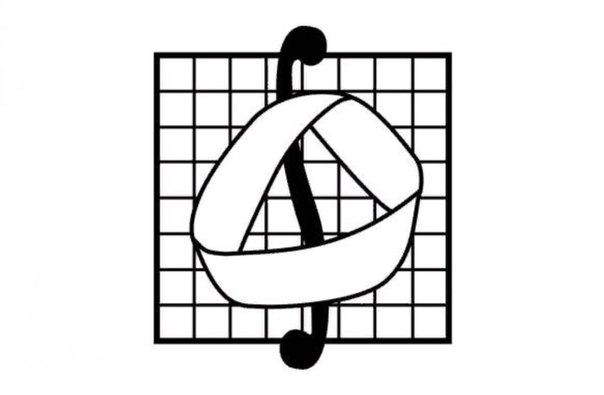
\includegraphics[scale=0.6]{mm.jpg} 
     
    Механико-математический факультет
    \vspace{0.25cm} 
      
    экономический поток
    \vspace{0.8cm} 
     
    {\LARGE МАТЕМАТИЧЕСКИЕ МЕТОДЫ В ЭКОНОМИКЕ}
    
    \vspace{0.8cm} 
    4 курс

    \vspace{0.25cm} 
    7 семестр
\end{center}
\vfill
 
\newlength{\ML}
\settowidth{\ML}{«\underline{\hspace{0.7cm}}» \underline{\hspace{1cm}}}
\hfill\begin{minipage}{7cm}
  \begin{flushright}
    Лектор $\;\;$\\
    к. ф.-м. н., доцент $\;\;$
    И.М.~Никонов $\;\;$\\
    «\underline{\hspace{0.7cm}}» \underline{\hspace{2cm}} 2021 г. $\;\;$
  \end{flushright}
\end{minipage}%
\vfill
\bigskip
 
\begin{center}
  Москва, 2021 г.
\end{center}
\tikz[remember picture,overlay] \node[opacity=0.1,inner sep=0pt] at (8.5,12.5){
\includegraphics[scale=0.8]{background1}};
\clearpage
\end{titlepage}
\newpage

\begin{center}
	{\Large \textbf{Техническая информация}}
\end{center}

\vspace{0.5cm}
Данный PDF содержит примерную программу осеннего семестра 4 курса по предмету <<Математические методы в экономике>>.

\vspace{0.5cm}
Собрали и напечатали по мотивам лекций и семинаров студенты 4-го курса Конов Марк и Гащук Елизавета.

\vspace{0.5cm}
Авторы выражают огромную благодарность лектору, кандидату ф.-м. наук, доценту Никонову Игорю Михайловичу за прочитанный курс по предмету <<Математические методы в экономике>>.

\vspace{0.5cm}
Добавления и исправления принимаются на почты \href{}{vkonov2@yandex.ru} и \\\href{}{gashchuk2011@mail.ru}.

\vspace{0.5cm}
\begin{center}
	{\Large \textbf{ПРИЯТНОГО ИЗУЧЕНИЯ}}
\end{center}

\newpage



\tableofcontents

\chapter{Предварительные сведения}\label{cha:1}

\section{Мера, распределение}\label{cha:1/sec:1}

Пусть $\Omega = \{ w\}$ - произвольное множество, а $\mathcal{F}$ - сигма-алгебра его подмножеств. Т.е. $\mathcal{F}$ такая система множеств, что:
\begin{itemize}
	\item[1)] $\Omega \in \mathcal{F}$
	\item[2)] если $A \in \mathcal{F}$, то $\overline{A} := \Omega - \mathcal{F} \in \mathcal{F}$
	\item[3)] если $A_1, A_2, \dots \in \mathcal{F}$, то $\underset{i}{\bigcup}A_i \in \mathcal{F}, \; \overset{i}{\bigcap}A_i \in \mathcal{F}$
\end{itemize}

\begin{definition}\label{cha:1/def:1}
	Пусть $\Omega = R$, а $\mathcal{F}$ - наименьшая сигма-алгебра, содержащая все интервалы $(\alpha, \beta)$. Такая $\mathcal{F}$ обозначается $\mathcal{B}(\mathbb{R})$ и называется \blue{борелевской} сигма-алгеброй.
\end{definition}

\begin{definition}\label{cha:1/def:2}
	Мера $\mu$, определенная на $\mathcal{F}$, называется \blue{сигма-аддитивной}, если:
	\begin{itemize}
		\item[1)] 
			это неотрицательная функция $\displaystyle \mu (A) \ge 0 \; \forall A \in \mathcal{F}$
		\item[2)] 
			она удовлетворяет условию сигма-аддитивности: $$\displaystyle \mu (\underset{i}{\overset{}{\sum}}A_i) = \underset{i}{\overset{}{\sum}}\mu(A_i), \; A_i \in \mathcal{F}, \; A_i A_j = \emptyset \text{ при } i \not = j$$
	\end{itemize}
\end{definition}

\begin{definition}\label{cha:1/def:3}
	Мера $\mu$ называется \blue{сигма-конечной}, если существуют множества $A_i \in \mathcal{F}$ такие, что $\underset{i}{\bigcup}A_i = \Omega$ и $\mu(A_i) < \infty$.
\end{definition}

\colorbox{DarkSeaGreen}{Считающая мера}: пусть $\Omega$ - счетное, $\mathcal{F}$ - множество всех подмножеств $\Omega$. Положим для $A \in \mathcal{F}$
$\displaystyle \mu(A) := \{ \text{число точек } \Omega, \text{ попавших в } A \}$. Такая мера $\mu$ называется считающей, она сигма-конечна.\\

\colorbox{DarkSeaGreen}{Лебегова мера}: пусть $\Omega = \mathbb{R}, \; \mathcal{F} = \mathcal{B}(\mathbb{R})$. Существует единственная мера $\mu$ на $\mathcal{B}(\mathbb{R})$ такая, что $\displaystyle \mu\left( (\alpha, \beta] \right) = \beta - \alpha$. Эта мера Лебега, она сигма-конечна.\\

\vspace{0.5cm}
$(\Omega, \mathcal{F})$ - измеримое пространство, $(\Omega, \mathcal{F}, \mu)$ - пространство с мерой.

\begin{definition}\label{cha:1/def:4}
	Если $\mu(\Omega) = 1$, то $\mu$ - \blue{вероятностная мера}, она обозначается через $P$. Тройка $(\Omega, \mathcal{F}, \mu)$ - \blue{вероятностное пространство}.
\end{definition}

\begin{definition}\label{cha:1/def:5}
	Измеримая функция $\xi: (\Omega, \mathcal{F}) \to (\mathbb{R}, \mathcal{B}(\mathbb{R}))$ называется \blue{случайной величиной}. Измеримость означает, что:
	$$\forall B \in \mathcal{B}(\mathbb{R}) \;\; \xi^{-1}(B) := (w \; : \; \xi(w) \in B) \in \mathcal{F}$$ Измеримая функция $\varphi: (\mathbb{R}, \mathcal{B}(\mathbb{R})) \to (\mathbb{R}, \mathcal{B}(\mathbb{R}))$ называется \blue{борелевской}.
\end{definition}

\begin{definition}\label{cha:1/def:6}
	Рассмотрим случайную величину $\xi \in \mathbb{R}^1$. Для $x \in \mathbb{R}^1$ функция $F(x) = P(w: \xi(w) \le x) = P(\xi \le x)$ называется \blue{функцией распределения}.
\end{definition}

\begin{definition}\label{cha:1/def:7}
	Мера $P_{\xi} (A) = P(w: \xi(w) \in A), \; A \in \mathcal{B}(\mathbb{R})$, называется \blue{распределением} случайной величины $\xi$.
\end{definition}

Тогда $F(x) = P_{\xi} \left( (-\infty, x] \right)$, т.е. $P_{\xi}$ определяет $F(x)$. 

Обратно: $P(\alpha < \xi \le \beta) = F(\beta) - F(\alpha)$, и существует единственная вероятностная мера $P_{\xi}$ такая, что $P_{\xi} \left( (\alpha, \beta] \right) = F(\beta) - F(\alpha)$, т.е. $F(x)$ определяет $P_{\xi}$.

\begin{definition}\label{cha:1/def:8}
	Пусть на $(\mathbb{R}, \mathcal{B}(\mathbb{R}))$ задана сигма-конечная мера $\mu$. Если существует борелевская функция $f(x), \; f(x) \ge 0$, такая, что
	$$P_{\xi} (A) = \underset{A}{\overset{}{\int}}f(x) \mu(dx) \;\; \forall A \in \mathcal{B}(\mathbb{R})$$
	то $f(x)$ называется \blue{плотностью} вероятности по мере $\mu$.
\end{definition}

Если $\mu$ - мера Лебега, то $f(x)$ - обычная плотность случайной величины $\xi$, введенная на 2-ом курсе. Если же $\xi$ дискретна со значениями $x_1, x_2, \dots$, а $\mu$ - считающая мера, сосредоточенная в этих точках, то, очевидно:
$$P_{\xi}(A) = \underset{A}{\overset{}{\int}}P(\xi = x)\mu(dx) \; \forall A \in \mathcal{B}(\mathbb{R})$$
Последнее равенство означает, что у дискретной случайной величины $\xi$ есть плотность вероятности $f(x) = P(\xi = x), \; x = x_1, x_2, \dots$ по считающей мере. При $x \not = x_1, x_2, \dots$ значения этой плотности не важны, их можно положить равными нулю.

\begin{definition}\label{cha:1/def:9}
	\blue{Математическим ожиданием} случайной величины $\xi$ называется число $E \xi = \underset{\Omega}{\overset{}{\int}}\xi(w) P(dw)$ в предположении, что $\underset{\Omega}{\overset{}{\int}}|\xi(w)|P(dw) < \infty$. Если $\underset{\Omega}{\overset{}{\int}}|\xi(w)|P(dw) = \infty$, то будем говорить, что $E \xi$ не существует.
\end{definition}

Если $f(x)$ - плотность вероятности случайной величины $\xi$ по мере $\mu$, а $\varphi(x)$ - борелевская функция, то:
$$E \varphi(x) = \underset{R}{\overset{}{\int}}\varphi(x) P_{\xi} (dx) = \underset{R}{\overset{}{\int}}\varphi(x) f(x) \mu(dx)$$
В частности, если $\xi$ - абсолютно непрерывная случайная величина в терминологии 2-го курса (т.е. $\mu$ - мера Лебега), то в случае $\underset{R}{\overset{}{\int}}|\varphi(x)|f(x) dx < \infty$ пишем $E \varphi(x) = \underset{R}{\overset{}{\int}}\varphi(x) f(x) dx$.

Если $\xi$ дискретна со значениями $x_1, x_2, \dots$ и соответствующими вероятностями $p_1, p_2, \dots$, то $E \varphi (\xi) = \underset{i \ge 1}{\overset{}{\sum}} \varphi (x_i) p_i$ (если ряд сходится абсолютно).

\section{Случайные вектора}\label{cha:1/sec:2}

Обозначим $\mathcal{B}(\mathbb{R}^k)$ борелевскую сигма-алгебру подмножеств $\mathbb{R}^n$.

\begin{definition}\label{cha:1/def:10}
	Вектор $\xi = (\xi_1, \dots, \xi_k)^T$ называется \blue{$k$-мерным случайным вектором}, если $\xi$ - измеримое отображение $\xi: (\Omega, \mathcal{F}) \to (\mathbb{R}^k, \mathcal{B}(\mathbb{R}^k)$
\end{definition}

Известно: $\xi$ - случайный вектор тогда и только тогда, когда каждая компонента $\xi_i$ - одномерная случайная величина.

\begin{definition}\label{cha:1/def:11}
	Функция распределения случайного вектора $\xi$: $F(x_1, \dots, x_k) = P(\xi_1 \le x_1, \dots, \xi_k \le x_k), \; x_i \in \mathbb{R}$, а распределение $P_{\xi}(A) = P(w: \xi(w) \in A), \; A \in \mathcal{B}(\mathbb{R}^k)$.
\end{definition}

\begin{definition}\label{cha:1/def:12}
	Плотность вероятности вектора $\xi$ по мере $\mu$ ($\mu$ распределена на элементам $\mathcal{B}(\mathbb{R}^k)$) - борелевская функция $f(x) \ge 0, \; x = (x_1, \dots, x_n)$, такая что:
	$$P_{\xi}(A) = \underset{A}{\overset{}{\int}}f(x) \mu (dx) \; \forall A \in \mathcal{B}(\mathbb{R}^k)$$
\end{definition}

\begin{definition}\label{cha:1/def:13}
	Случайные величины $\{\xi_1, \dots, \xi_k\}$ независимы, если
	$$P(\xi_1 \in A_1, \dots, \xi_k \in A_k) = \underset{i=1}{\overset{k}{\Pi}} P(\xi_i \in A_i) \; \forall A_i \in \mathcal{B}(\mathbb{R})$$
\end{definition}

\begin{propose}[\textit{необходимые и достаточные условия независимости}]\label{cha:1/propose:1}
	$$F(x_1, \dots, x_k) = F_{\xi_1} (x_1) F_{\xi_2}(x_2) \dots F_{\xi_k}(x_k) \; \forall (x_1, \dots, x_k)$$
	$$f(x_1, \dots, x_k) = f_{\xi_1}(x_1)\dots f_{\xi_k}(x_k)$$
\end{propose}

\section{Сходимости случайных векторов}\label{cha:1/sec:3}

Пусть случайные векторы $\xi, \xi_1, \xi_2, \dots$ размера $k$ со значениями в $(\mathbb{R}^k, \mathcal{B}(\mathbb{R}^k))$ определены на некотором вероятностном пространстве $(\Omega, \mathcal{F}, P)$. Пусть $|\cdot|$ означает евклидову норму вектора, т.е. $|\xi| = \sqrt{\xi_1^2 + \dots + \xi_k^2}$.

\begin{definition}\label{cha:1/def:14}
	Говорят, что последовательность $\{\xi_n\}$ \blue{сходится слабо} к $\xi$ ($\xi_n \xrightarrow[n\to \infty]{W} \xi$), если для любой непрерывной и ограниченной функции $g: \mathbb{R}^k \to \mathbb{R}^1$ имеет место сходимость:
	$$\underset{\mathbb{R}^k}{\overset{}{\int}}g(x) P_n(dx) \xrightarrow[n \to \infty]{}\underset{\mathbb{R}^k}{\overset{}{\int}}g(x) P(dx)\eqno(1)$$
	($P_n$ и $P$ - распределения $\xi_n$ и $\xi$ соотвественно)
\end{definition}

\begin{definition}\label{cha:1/def:15}
	Обозначим $F_n(x)$ и $F(x), \; x = (x_1, \dots, x_n)$, функции распределения векторов $\xi_n$ и $\xi$. Тогда сходимость $(1)$ эквивалентна \blue{сходимости в основном}:
	$$F_n(x) \Rightarrow F(x) \; \Leftrightarrow \; F_n(x) \to F(x) \;\; \forall x \in \mathbb{C}(\mathcal{F})\eqno(2)$$
\end{definition}

\begin{definition}\label{cha:1/def:16}
	Пусть $\varphi_n(t)$ и $\varphi(t), \; t \in \mathbb{R}^k$, будут характеристические функции $\xi_n$ и $\xi$, т.е. $\varphi(t) := E e^{i t^T \xi}$. Тогда сходимость $(2)$ эквивалентна сходимости:
	$$\varphi_n (t) \xrightarrow[n \to \infty]{}\varphi(t) \;\; \forall t \in \mathbb{R}^k\eqno(3)$$
\end{definition}

\begin{definition}\label{cha:1/def:17}
	Если выполнено любое из соотношений $(1)-(3)$, будем писать:
	$$\xi_n \xrightarrow[n \to \infty]{d}\xi\eqno(4)$$
	и говорить, что $\{\xi_n\}$ сходится к $\xi$ \blue{по распределению}.
\end{definition}

\begin{remark}\label{cha:1/remark:1}
	Сходимость $(4)$ не следует из сходимости $\xi_{in} \xrightarrow[]{d}\xi_i, \; i = 1, \dots, k$, компонент векторов $\xi_n$ и $\xi$.
\end{remark}

\begin{definition}\label{cha:1/def:18}
	Говорят, что последовательность $\{\xi_n\}$ сходится \blue{по вероятности} к вектору $\xi$ ($\xi_n \xrightarrow[n \to \infty]{P}\xi$), если:
	$$\forall \varepsilon > 0 \;\; P(|\xi_n - \xi| > \varepsilon) \xrightarrow[n \to \infty]{}0 \eqno(5)$$
\end{definition}

\begin{remark}\label{cha:1/remark:2}
	Понятно, что сходимость $(5)$ эквивалентна сходимости компонент $\xi_{in} \xrightarrow[]{P} \xi_i$ для всех $i=1,2,\dots, k$.
\end{remark}

\begin{remark}\label{cha:1/remark:3}
	Сходимость по вероятности $(5)$ влечет сходимость по распределению $(4)$. Обратное верно только в частных случаях.
\end{remark}

\begin{definition}\label{cha:1/def:19}
	Говорят, что последовательность $\{\xi_n\}$ \blue{сходится п.н.} (почти наверно или с вероятностью единица) и пишут $\xi_n \xrightarrow[n\to \infty]{\text{п.н.}}\xi$, если:
	$$P(w:\xi_n(w) \to \xi(w)) = 1\eqno(6)$$
\end{definition}

\begin{remark}\label{cha:1/remark:4}
	Сходимость п.н. $(6)$ влечет сходимость по вероятности $(5)$. Значит верна следующая цепочка:
	$$\xi_n \xrightarrow[n\to \infty]{\text{п.н.}}\xi \; \Rightarrow \; \xi_n \xrightarrow[n \to \infty]{P}\xi \; \Rightarrow \; \xi_n \xrightarrow[n \to \infty]{d}\xi$$
\end{remark}

\begin{theorem}[\red{непрерывности}]\label{cha:1/the:1}
	Пусть векторы $\{\xi_n\}, \xi$ определены на $(\Omega, \mathcal{F}, P), \;\; \xi_n, \xi \in \mathbb{R}^k$. Пусть $A \in \mathcal{B}(\mathbb{R}^k)$ и $P(\xi \in A) = 1$ (т.е. $A$ - носитель $\xi$). Пусть борелевская $H: \mathbb{R}^k \to \mathbb{R}^1$ непрерывна на множестве $A$. Тогда:
	\begin{itemize}
		\item[1)] если $\xi_n \xrightarrow[n \to \infty]{d}\xi$, то $H(\xi_n)\xrightarrow[n \to \infty]{d}H(\xi)$
		\item[2)] если $\xi_n \xrightarrow[n \to \infty]{P}\xi$, то $H(\xi_n)\xrightarrow[n \to \infty]{P}H(\xi)$
		\item[3)] если $\xi_n \xrightarrow[n \to \infty]{\text{п.н.}}\xi$, то $H(\xi_n)\xrightarrow[n \to \infty]{\text{п.н.}}H(\xi)$
	\end{itemize}
\end{theorem}
\begin{Proof}
	Докажем пункт 3. Два других пункта будут доказаны на практических занятиях.

	Итак, в силу непрерывности функции $H(x)$ на $A$:
	$$\begin{gathered}
		(w:\xi_n(w) \to \xi(w)) \cap (w: \xi(w)\in A) \subseteq (w: H(\xi_n(w))) \to H(\xi(w)) \; \Rightarrow \\
		\Rightarrow \; 1 = P(\xi_n(w) \to \xi(w)) = P(\xi_n(w) \to \xi(w), \xi(w) \in A) \le P(H(\xi_n(w)) \to H(\xi(w))) 
	\end{gathered}$$
\end{Proof}

\section{ЗБЧ и ЦПТ}\label{cha:1/sec:4}

Пусть на $(\Omega, \mathcal{F}, P)$ задана бесконечная последовательность случайных величин $\xi_1, \xi_2, \dots$

\begin{definition}\label{cha:1/def:20}
	Если $\{\xi_i\}$ независимы и одинаково распределены с конечным средним, $E|\xi_1| < \infty$, то
	$$n^{-1} \underset{i=1}{\overset{n}{\sum}}\xi_i \xrightarrow[n\to \infty]{\text{п.н.}}E \xi_1\eqno(7)$$
	Соотношение $(7)$ - \blue{усиленный закон больших чисел Колмогорова}.
\end{definition}

\begin{definition}\label{cha:1/def:21}
	Если $\{\xi_i\}$ некоррелированные случайные величины, может быть, разнораспределенные, но с одинаковым средним $m = E \xi_i$ и $D \xi_i \le C < \infty$, то
	$$n^{-1}\underset{i=1}{\overset{n}{\sum}}\xi_i \xrightarrow[n \to \infty]{P}m = E \xi_i\eqno(8)$$
	Соотношение $(8)$ - \blue{слабый закон больших чисел}.
\end{definition}

\begin{definition}\label{cha:1/def:22}
	Если $\{\xi_i\}$ - н.о.р.с.в., $E \xi_1 = m, \; 0 < D\xi_1 = \sigma^2 < \infty$, то
	$$\frac{1}{\sqrt{n}\sigma} \underset{i=1}{\overset{n}{\sum}}(\xi_i - m) \xrightarrow[n \to \infty]{d}\xi \sim N(0,1)\eqno(9)$$
	Соотношение $(9)$ - \blue{центральная предельная теорема}, точнее ее вариант, т.е.:
	$$n^{\frac{1}{2}} (\overline{\xi} - m)\xrightarrow[n \to \infty]{d}N(0, \sigma^2), \text{ где } \overline{\xi} := n^{-1} \underset{i=1}{\overset{n}{\sum}}\xi_i$$
\end{definition}




\chapter{Статистическая модель}\label{cha:2}

\section{Оценка среднего}\label{cha:2/sec:1}
\begin{example}[\red{оценка среднего}]
	Будем предполагать, что на некотором вероятностном пространстве $ (\Omega, \mathcal{F}, P)$ определена бесконенчая последовательность $ X_1, X_2, ...$ и $ X_1, ... , X_n$ - ее первые n членов. Интересующий нас параметр, определеяющий (в какой-то мере) срок службы, отождествим $ \theta = EX_1$.

	Одна из стандратных статистических задач состоит в том, чтобы выяснить, чему равно $ \theta.$
	Вот возможное решение.
	В силу УЗБЧ Колмогорова
	$$\overline{X} = \frac{1}{n}\sum\limits_{i=1}^{n}\xrightarrow[n\to \infty]{\text{п.н.}}EX_1 = \theta$$
	Возьмем n готовых изделий и проверим их. Пусть $ x_1, x_2, ..., x_n$ - сроки службы готовых изделий. Это реализации сл.в. $ X_1, ..., X_n.$ Естественно ожидать, что $ \displaystyle \overline{X}  = \frac{1}{n}\sum\limits_{i=1}^{n}x_i$ при больших n окажется близким к $ \theta.$ Это \blue{задача точечного оценивания параметра}: пусть $ X_1, .. ,X_n- $ случайные наблюдения; $ \overline{X}-  $ статистическая оценка( это случайная величина); $ \overline{x}$ - реализация оценки, с ней обычно работают на практике.

	Ясно, что нужны оценки, которые в среднем близки к $ \theta.$ Тогда и реализации будут близки.

	Пусть в частности 
	$\displaystyle P(X_1 \le t) = \begin{cases}
		0, \; t \leq 0\\
		1 - e^{-\frac{t}{\theta}}, \; t>0
	\end{cases}$, параметр $ \theta > 0$. Т.е. $ X_1 \sim exp(\frac{1}{\theta})$ и $ E_{\theta}X_1 = \theta.$

	Тогда $ \overline{X} $ \textbf{оптимальна} при любом n > 0 в следующем смысле.
	\begin{itemize}
			\item[1)] 
				$\displaystyle E_{\theta}\overline{X} = \frac{1}{n}\sum\limits_{i=0}^{n}E_{\theta}X_i = \theta \; \forall \theta > 0$ - это свойство \blue{несмещенности}. Качественно: реализации $ \overline{x}$ группируются вокруг $ \theta$.
			\item[2)] 
				$\displaystyle D_{\theta}\overline{X} \leq D_{\theta} \hat{\theta}_n, \; \theta > 0$ и любой несмещенной оценки $ \hat{\theta}_n = \hat{\theta}_n(X_1, \dots, X_n).$ Качественно: реализации $  \overline{X}$ в среднем лежат ближе к $ \theta$, чем у других $ \hat{\theta}_n$.
		\end{itemize}	
\end{example}

\section{Проверка однородности данных}\label{cha:2/sec:2}
\begin{example}[\red{проверка однородности данных}]
	Пусть некоторый эксперимент проводится сначала $ m$ раз в условиях $A$, а затем $ n$ раз в условиях $ B$ (например, влияет ли некоторый препарат на на развитие растений, лекарство на анализы больного и т.д.).

	\noindent Будем считать $ {x_i}$ реализациями н.о.р.с.в. $ {X_i} $ c функцией распредления $ X_1 \sim F_X(x) = P(X_1 \leq x).$ Пусть $ {y_i}$ - реализации н.о.р.с.в. $ {Y_i}$, ф.р. $ Y = F_Y(x).$ Последовательности $ {x_i}, {y_i}$ независимы.

	\noindent Интерпретируем поставленную задачу как проверку гипотезы $\displaystyle H: F_X = F_Y$.
	Предположение о том, что условие $B$ дает другой результат интерпретируем как гипотезу (альтернативную к $ H$)
	$\displaystyle K: F_X \neq F_Y$.

	\textbf{Важно}: ни $ F_X$, ни $ F_Y$ неизвестны!

	\noindent Оценкой $ F_X$ возьмем $\displaystyle \hat{F}_{mX}(x) = \frac{1}{m}\sum\limits_{i=1}^{m}I(X_i \leq x), \; x \in \mathbb{R}$ - это <<хорошая>> оценка, т.к. в силу УЗБЧ: $\displaystyle \hat{F}_{mX}(x) \xrightarrow{\text{п.н.}}\; EI(X_1 \leq x) = F_X(x)$ $($у нас $ \{X_i\}$ и $ \{Y_i\}$ определены на одном $ (\Omega, \mathcal{F}, P)$$)$.

	\begin{theorem}[\red{Глиненко-Кантелли}]
		\[ \sup\limits_x|\hat{F}_{mX}(x) - F_X(x)| \xrightarrow[m \to \infty]{\text{п.н.}}
		0\]
	\end{theorem}

	Очевидно, если гипотеза $ H$ верна, то величина $\displaystyle D_{mn} := \sup\limits_x|\hat{F}_{mX}(x) -\hat{F}_{nY}(x)|$ мала при больших $ m,n.$
	Вот естественное правило:
	\begin{itemize}
		\item[$\bullet$] $\text{если } D_{mn}\leq c, \text{ то } H \text{ принять }$
		\item[$\bullet$] $\text{если } D_{mn}> c, \text{то } H \text{ отвергнуть и принять } K$
	\end{itemize}

	\textbf{Но как выбрать константу с?}
	\begin{lemma}
		Пусть верна гипотеза $H$ и $F_X = F_Y = F$. Пусть $F$ непрерывна. Тогда распределение сл.в. $D_{mn}$ не зависит от $F(x)$ при любом $x$ и конечных $m,n$.
	\end{lemma}
	\begin{Proof}
		Докажем лемму при дополнительном предположении: $F(x)$ строго возрастает. Тогда при любом $t \in (0,1)$ существует $F^{-1}(t)$, и эта функция непрерывна и строго возрастает. Сделаем замену переменной $F(x) = t, \; x =F^{-1}(t)$. Тогда при $x \in \mathbb{R}$ переменная $t \in (0,1)$ и 
		\[D_{mn} = \sup\limits_{t \in (0,1)}|\hat{F}_{mX}(F^{-1}(t)) -\hat{F}_{nY}(F^{-1}(t))|.\]
		Но $\displaystyle \hat{F}_{mX}(F^{-1}(t)) = \frac{1}{m}\sum\limits_{i=1}^{m}I(X_i \leq F^{-1}(t)) = \frac{1}{m}\sum\limits_{i=1}^{m}I(F(X_i)\leq t)$, т.к.\\ $ (X_i \leq F^{-1}(t)) = (F(X_i)\leq t)$. Осталось заметить, что если $X_i \sim F(x)$ и $F(x)$ строго возрастает, то $\displaystyle F(X_i)	=\eta_i \sim R(0,1)$.

		\noindent Действительно, 
		$\displaystyle \forall t \in (0,1) \;\; P(F(X_i) \leq t) = P(X_i \leq F^{-1}(t)) = F(F^{-1}(t)) = t$.

		\noindent Значит $\displaystyle \hat{F}_{mX}(F^{-1}(t)) = \frac{1}{m}\sum\limits_{i=1}^{m}I(\eta_i \leq t)$,
		где $ {\eta_i}$ - н.о.р. $ R(0,1)$ сл.в., а тогда $\hat{F}_{mX}(F^{-1}(t))$ имеет ф.р., которая от $F(x)$ не зависит. Для $\hat{F}_{nY}(F^{-1}(t))$ имеем то же самое. 
	\end{Proof}

	\vspace{0.3cm}
	Если $D_{mn}$ свободно от $F(x)$ (при $H$), то его можно вычислить при любых $m,n$. Например, полагая, что $X_1, .., X_m$ и $Y_1, .., Y_n$ распределены как $R(0,1)$. Но особенно красив ответ при $m,n \rightarrow  \infty$.

	\begin{theorem}[\red{Смирнова}]
		Пусть $H$ верна. Пусть $F_X = F_Y =F$, и $F$ непрерывна. Тогда при $\lambda > 0$
		\[ \lim\limits_{m,n \rightarrow \infty}P(\sqrt{\frac{mn}{m+m}D_{mn}}< \lambda) = K(\lambda),\]
		где $ K(\lambda) = 1 - 2 \sum\limits_{j\geq1}(-1)^{j+1}e^{-2j^2\lambda^2} $ - \blue{функция распредления Колмогорова}.
	\end{theorem}
	
	Выберем малое $0<\alpha<1$ и пусть $\lambda_{1-\alpha}$ такое число, что $K(\lambda_{1-\alpha}) = 1- \alpha$ . Число $\lambda_{1-\alpha}$ называют \red{квантилью уровня} $1-\alpha$.

	Положим $\displaystyle c_{\alpha}(m,n) =\sqrt{\frac{m+n}{mn}\lambda_{1-\alpha}}$ - это и есть искомая константа с!

	\textbf{Правило}:
	$\displaystyle \begin{cases}
		\text{если } D_{mn}\leq c_{\alpha}(m,n), \text{ то } H \text{ принимаем }\\
		\text{если } D_{mn}> c_{\alpha}(m,n), \text{ то принимаем } K
	\end{cases}$

	Тогда вероятность \red{ошибки первого рода}:
	\begin{gather*}
		P(K|H) = P(\sqrt{\frac{mn}{m+n}}D_{mn} > \lambda_{1-\alpha}) =\\
		=1 - P(\sqrt{\frac{mn}{m+n}}D_{mn}\leq \lambda_{1-\alpha}) \rightarrow 1 - K(\lambda_{1-\alpha}) = \alpha
	\end{gather*}
	Можно показать, что $P(H|K) \to 0$ при $m,n \to \infty$. Это вероятность \red{ошибки 2-ого рода}.

	Итак, $\displaystyle \begin{cases}
			P(H|H) \rightarrow \; 1-\alpha\\
			P(K|K) \rightarrow \; 1
		\end{cases}$\\
	(т.е. тест с большой вероятностью выберет правильную гипотезу!)
\end{example}
% chapter примеры_статистических_задач_статистическая_модель (end)

\chapter{Теорема Гливенко-Кантелли. Метод подстановки} % (fold)

\section{Теорема Гливенко-Кантелли}\label{lec:3/sec:1}

Пусть  $X=(X_1, \dots, X_n)$ - случайный вектор наблюдений. Дальше $n$ будет расти. Поэтому предполагается, что на некотором вероятностном пространстве $(\Omega, \mathcal{F}, P)$ определена бесконечная последовательность н.о.р. случайных величин $X_1, X_2, \dots$ с неизвестной функцией распределения $F(x)$. Наблюдение $X$ содержит первые $n$ компонент этой последовательности.

Наша цель - оценить $F(x) = P(X_1 \leq x), x \in \mathbb{R}$. Зафиксируем $\omega \in \Omega$ и рассмотрим реализации $\displaystyle x_k = X_k(\omega), \;k=1,\dots, n$.
Пусть $\displaystyle x_{(1)}\leq x_{(2)} \leq \dots\leq x_{(n)}$.
\begin{definition}
	Случайная величина $X_{(k)}$, равная на упомянутом $\omega$
	$\displaystyle X_{(k)}(\omega)= x_{(k)}, \;k = 1, 2, \dots, n$
	называется \red{к-ой порядковой статистикой}.
	Совокупность $\displaystyle X_{(1)}\leq X_{(2)} \leq...\leq X_{(n)}$
	называется \red{вариационным рядом}.
\end{definition}

\begin{definition}
	Оценкой $F(x)$ в точке $x$ возьмем $\hat{F}_n(x) = \frac{1}{n}\sum\limits_{i=0}^{n}I(X_i \leq x)$, где $I$ - индикатор.
	$\hat{F}_n(x)$ называется \red{эмпирической функцией распределения}.
\end{definition}

Если $x_{(1)}\leq x_{(2)} \leq \dots \leq x_{(n)}$ - реализация вариационного ряда, то график реализации $\hat{F}_n(x)$ такой:
\begin{multicols}{2}

	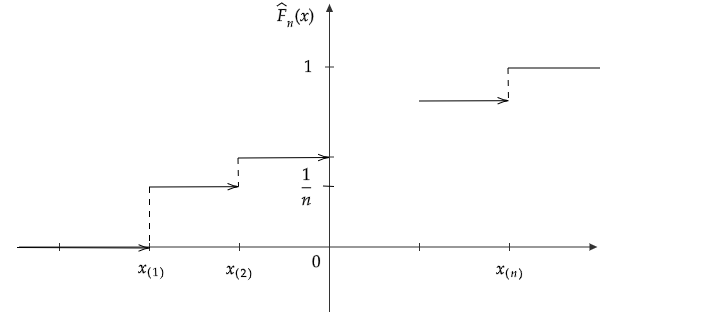
\includegraphics[height=5cm,width=10cm]{lec3im1}

	\columnbreak
	\hfill \break

	При каждом $\omega$ $\hat{F}_n(x) =\hat{F}_n(x, \omega)$ - дискретная ф.р. 

	При фиксированном $ x \;\; \hat{F}_n(x)$ - случайная величина.
\end{multicols}

В силу УЗБЧ: $\displaystyle \frac{1}{n}\sum\limits_{i=0}^{n}I(X_i \leq x) \xrightarrow[n \to \infty]{\text{п.н.}} EI(X_1 \leq x) = F(x)$.

В силу ЦПТ: $\displaystyle \frac{1}{n}(\hat{F}_n(x)- F(x))=\frac{1}{\sqrt{n}}\sum\limits_{i=0}^{n}(I(X_i \leq x)- F(x)) \;\xrightarrow[n \to\infty]{d}  N(0, \hat{F}_n(x)- F^2(x))$, т.к. $ DI(X_1 \leq x) = EI^2(X_1 \leq x) -(EI(X_1 \leq x))^2 = F(x) - F^2(x)$.
\vspace{1cm}

Докажем следующую важнейшую теорему:

\begin{theorem}[\red{Гливенко-Кантелли}]
	Пусть $X_1, \dots, X_n$ - н.о.р.с.в., $X_1 \sim F(x)$. Тогда 
	$$ \sup\limits_x|\hat{F}_n(x)-F(x)| \xrightarrow[n\to\infty]{\text{п.н.}}
	0$$
\end{theorem}
\begin{Proof}
	Пусть $F(x)$ непрерывна. Пусть $\varepsilon > 0$ - любое малое число, такое что $N = \frac{1}{\varepsilon}$ - целое. Выберем точки $\displaystyle -\infty= z_0<z_1< \dots < z_{N-1}<z_N=\infty$
	так что $\displaystyle F(z_k) = \frac{k}{N}, k = 0,1, \dots,N$. 
	Для $x \in [z_k, z_{k+1})$ в силу монотонности $\hat{F}_n(x)$ имеем:
	$$\hat{F}_n(x) - F(x)\leq \hat{F}_n(z_{k+1})-F(z_k) = \hat{F}_n(z_{k+1})- F(z_{k+1}) + \varepsilon \leq \max\limits_k|\hat{F}_n(z_{k}) - F(z_k)| + \varepsilon$$
	$$\hat{F}_n(x) - F(x) \geq  \hat{F}_n(z_{k})-F(z_{k+1}) = \hat{F}_n(z_{k}) - F(z_k) - \varepsilon \geq -\max\limits_k|\hat{F}_n(z_{k}) - F(z_k)| + \varepsilon$$
	Из двух последних неравенств получаем:
	$$\sup\limits_x|\hat{F}_n(x) - F(x)| \leq \max\limits_k|\hat{F}_n(z_{k}) - F(z_k)| + \varepsilon \eqno(1)$$
	Пусть $\displaystyle A_k = \{ \omega : \hat{F}_n(z_{k}) \rightarrow F(z_k) \}$. Тогда $\displaystyle P(A_k) = 1$. Пусть $\displaystyle A = \bigcap\limits_kA_k$. Тогда $\displaystyle \forall \omega \in A \; \max\limits_k|\hat{F}_n(z_{k}) - F(z_k)|\to 0$. Значит: 
	$$\forall \omega \in A \; \exists n_0=n_0(\omega): \; n > n_0 \;\; \max\limits_k|\hat{F}_n(z_{k}) - F(z_k)|<\varepsilon\eqno(2)$$
	В силу (1) и (2) для этого $\omega$ при $n>n_0$ получаем, что:
	$$\sup\limits_x|\hat{F}_n(x) - F(x)| < 2\varepsilon\eqno(3)$$
	Так как $P(A)=1$ и $\varepsilon$ произвольно, то (3) означает $\displaystyle \sup\limits_x|\hat{F}_n(x) - F(x)| \xrightarrow[n\to\infty]{\text{п.н.}}0$.
\end{Proof}

\begin{problem}
	Доказать теорему Гливенко-Кантелли для разрывной $F(x)$.
\end{problem}
$($см. [А.А.Боровков. Математическая статистика. Оценка параметров и проверка гипотез. М., Наука, 1984 г.]$)$

\section{Метод подстановки}\label{lec:3/sec:2}
Пусть надо оценить параметр $\theta = G(F)$, $G(\cdot)$ - функционал на множестве функций распределения. Естественная оценка подставновки $\displaystyle \hat{\theta}_n = G(\hat{F}_n)$.

\begin{example}
	Пусть $\displaystyle E|X_1|^k<\infty,\;\; \nu_k=EX_1^k,\; k\in \mathbb{N}$. $\nu_k$ называют \red{к-ым начальным моментом}. Тогда $\displaystyle \nu_k = G(F) = \int\limits^{\infty}_{-\infty}x^kdF(x)$.
	Оценка подстановки для $\theta = \nu_k$: $\displaystyle \;\;\;\;\; \hat{\theta}_n = \hat{\nu}_k = \int\limits^{\infty}_{-\infty}x^kd\hat{F}_n(x) = \frac{1}{n}\sum\limits_{i=1}^{n}X_{(i)}^k = \frac{1}{n}\sum\limits_{i=0}^{n}X_i^k$.\\
	В силу УЗБЧ: $\displaystyle \;\;\;\;\; \hat{\nu}_k = \frac{1}{n}\sum\limits_{i=0}^{n}X_i^k \xrightarrow[n\to\infty]{\text{п.н.}} EX_1^k=\nu_k$.\\
	Кроме того, при $EX_1^{2k} < \infty$ имеем в силу ЦПТ:
	$$\sqrt{n}(\hat{\nu}_k - \nu_k) =\frac{1}{\sqrt{n}}\sum\limits_{i=1}^{n}(X_i^k-\nu_k) \xrightarrow{d}\; N(0, \nu_{2k} - \nu_k^2),\;n\rightarrow\infty$$  
	Значит $\displaystyle (\nu_{2k} - \nu_k^2)^{-\frac{1}{2}}\sqrt{n}(\hat{\nu}_k - \nu_k) \rightarrow N(0,1)$. Отсюда:
	$$\forall \varepsilon >0 \; P\left((\nu_{2k} - \nu_k^2)^{-\frac{1}{2}}|\sqrt{n}(\hat{\nu}_k - \nu_k)| \leq \varepsilon\right)\rightarrow\Phi(\varepsilon)-\Phi(-\varepsilon) =2\Phi(\varepsilon)-1 \eqno(4)$$
	где $ \Phi(x)=\frac{1}{\sqrt{2\pi}}\int\limits^{\infty}_{-\infty}e^{-\frac{t^2}{2}}dt$ - функция Лапласа.
	Асимптотическая нормальность позволила оценить в $(4)$ точность оценки $\hat{\nu}_k$.
\end{example}

\begin{example}[\blue{Выборочные квантили}]
	Для $0<p<1$ и любой (не обязательно непрерывной) функции распредления $F(x)$ полагают $\displaystyle F^{-1}(p) \equiv \sup{x: F(x) \leq p}$.
	Величина $F^{-1}(p)$ называется \red{квантилью} функции распределения $F(x)$ и обозначается далее $\xi_p$.

	Если $F(x)$ непрерывна и строго возрастает, то $F(\xi_p) = p$.
\end{example}

Пусть $\displaystyle X_{(1)}\leq X_{(2)} \leq \dots \leq X_{(n)}$
- вариационный ряд выборки $X_1, \dots, X_n$. Оценка $\xi_p$ по методу подстановки:
$$\hat{\xi}_p = \hat{F}_n^{-1}(p) = sup\{x: \hat{F}_n{x} \leq p \} = X_{([np]+1)}$$

\begin{lemma}
	Пусть функция распределения $F(x)$ непрерывна и строго возрастает. Тогда функционал $G(F) = \xi_p, \; 0<p<1$ непрерывен в равномерной метрике. Т.е., если последовательность ф.р. ${F_n(x)}$ такова, что $\displaystyle \sup\limits_x|F_n(x) - F(x)|\rightarrow0$, то $\displaystyle G(F_n)\rightarrow G(F)$.
\end{lemma}
\begin{Proof}
	$\forall\;\varepsilon>0$ при $n>n_0(\varepsilon)$ имеем:
	$$\begin{gathered}
		G(F_n) \equiv \xi_p^n = \sup{x: F_n(x) \leq p} = \sup{x: F(x) \leq F(x) - F_n(x)+p}\leq \\ 
		\le \sup{x: F(x) \leq \sup\limits_y|F_n(y)-F(y)|+p} \leq \sup{x: F(x)\leq p+\varepsilon} = F^{-1}(p+\varepsilon) 
	\end{gathered}$$
	Аналогично: $\displaystyle \xi_p^n \geq F^{-1}(p-\varepsilon),\;n>n_0$. Значит $\displaystyle F^{-1}(p-\varepsilon)\leq\xi_p^n\leq F^{-1}(p+\varepsilon),\;n>n_0$. Тогда $\displaystyle F^{-1}(p-\varepsilon)\leq \underset{n\to\infty}{\underline{\lim}}\xi_p^n\leq \underset{n\to\infty}{\overline{\lim}}\xi_p^n \leq F^{-1}(p+\varepsilon)$.
	Функция $F^{-1}(t),\;0<t<1$ непрерывна. Устремляя $\varepsilon$ к нулю получим:
	$$\xi_p=\underline{\lim}_{n\rightarrow\infty}\xi_p^n\leq\overline{\lim}_{n\rightarrow\infty}\xi_p^n=\xi_p, \text{ т.е. } \lim\limits_{n\rightarrow\infty}\xi_n^p=\xi_p$$
\end{Proof}

\begin{conseq}
	Если $F(x)$ непрерывна и строго возрастает, то $\displaystyle \hat{\xi}_p \xrightarrow[n\rightarrow\infty]{\text{п.н.}} \xi_p$. Это прямо следует из \blue{теоремы Гливенко-Кантелли}.
\end{conseq}
\begin{definition}
	Величина $\xi_{\frac{1}{2}}$ называется \red{медианой}, а $\hat{\xi}_{\frac{1}{2}}$- \red{ выборочной медианой}.
\end{definition}

\begin{theorem}
	Пусть $F(x)$ дифференциируема в точке $\xi_{\frac{1}{2}}$, и $g(\xi_{\frac{1}{2}})\equiv F'(\xi_{\frac{1}{2}})>0$. Тогда:
	\[\sqrt{n}(\hat{\xi}_{\frac{1}{2}}-\xi_{\frac{1}{2}})\xrightarrow{d}N(0,\frac{1}{4g^2(\xi_{\frac{1}{2}})}),\;\;n\rightarrow\infty. \]
\end{theorem}

\section{Асимптотическая относительная эффективность оценок (АОЭ)}\label{lec:3/sec:3}

Асимптотически нормальные оценки можно сравнивать между собой.

Пусть по вектору наблюдений $X = (X_1, \dots, X_n)$ оценивается параметр $\theta$, и $\hat{\theta}_{1n}$ - его оценка. Пусть
$$\sqrt{n}(\hat{\theta}_{1n} - \theta) \xrightarrow[n\to\infty]{d} N(0, \sigma^2(\theta))\eqno(5)$$
Пусть есть другая оценка $\hat{\theta}_{2n}$, такая что:
$$\sqrt{n}(\hat{\theta}_{1n'} - \theta) \xrightarrow[n\to\infty]{d} N(0, \sigma^2(\theta))\eqno(6)$$
где $n'=n'(n) \xrightarrow[n\to\infty]{} \infty$.

\begin{definition}
	\red{Асимптотической относительной эффективностью} (АОЭ) оценки $\hat{\theta}_{1n}$ относительно оценки $\hat{\theta}_{2n}$ называется величина
	\[l_{1,2} \equiv \lim\limits_{n\rightarrow\infty}\frac{n'(n)}{n}.\]
\end{definition}

Пусть, например, $l_{1,2}=3$ . Тогда при больших $n$ $n'\approx3n$. Значит, для $\hat{\theta}_{2n}$ нужно в три раза больше наблюдений, чем для $\hat{\theta}_{1n}$, чтобы достичь одинаковой точности $\sigma^2(\theta)/n$. Оценка $\hat{\theta}_{1n}$ в три раза лучше оценки $\hat{\theta}_{2n}$.

\begin{lemma}
	Пусть $\displaystyle \sqrt{n}(\hat{\theta}_{in} - \theta)\xrightarrow[n\to\infty]{d}N(0,\sigma^2_i(\theta)),\; \sigma^2_i(\theta)>0, \; i = 1,2$.
	Тогда АОЭ существует и равна
	\[l_{1,2} = \frac{\sigma^2_2(\theta)}{\sigma^2_1(\theta)}.\]
\end{lemma}

\begin{proof}
	Пусть $n'\sim \frac{\sigma^2_2(\theta)}{\sigma^2_1(\theta)}n,\;\;n\rightarrow\infty$. Тогда
	$$\begin{gathered}
		\sqrt{n}(\hat{\theta}_{2n'}-\theta) = \sqrt{\frac{n}{n'}}\sqrt{n'}(\hat{\theta}_{2n'}-\theta) \xrightarrow{d} \frac{\sigma_2(\theta)}{\sigma_1(\theta)}\xi, \;\;\xi\sim N(0,\sigma^2_2(\theta)) \\
		(\text{использовали \blue{лемму Слуцкого}: если } \xi_n \xrightarrow{d}\xi,\; \eta_n \xrightarrow{d} c, \text{ то }\xi_n\eta_n \xrightarrow{d} c\xi)
	\end{gathered}$$
	Значит: $\displaystyle \sqrt{n}(\hat{\theta}_{2n'}-\theta) \xrightarrow{d} N(0,\sigma^2_1(\theta))$. Получаем: $\displaystyle \lim\limits_{n\rightarrow\infty} \frac{n'(n)}{n}=\frac{\sigma^2_2(\theta)}{\sigma^2_1(\theta)}$.
\end{proof}

\begin{example}[Важный]
	Пусть $\displaystyle X_i = \theta + \varepsilon_i, \;\; i=1,..,n,\;\; {\varepsilon_i}-\text{ н.о.р.}$. Пусть $\displaystyle E\varepsilon_1 = 0, \;\; D\varepsilon_1 = \sigma^2 < \infty$. Тогда $EX_1 = \theta$, и оценкой $\theta$ можно взять $\overline{X}= \frac{1}{n}\sum\limits_{i=1}^{n}X_i$. Знаем, что $\displaystyle \sqrt{n}(\overline{X}- \theta) \xrightarrow[n\to\infty]{d} N(0, \sigma^2)$, т.к. $\nu_2- \nu_1^2 = \sigma^2$.
\end{example}

Пусть теперь $\varepsilon_1$ имеют ф.р. $G(x)$ и существует плотность вероятности $g(x) = G'(x)$. Пусть $g(x) = g(-x)$ и $g(0)>0$. Тогда $G(0)=\frac{1}{2}$. Значит ф.р. $X_1$ имеет вид: $\displaystyle \;\;\; P(X_1 \leq \theta) = P(\theta+\varepsilon_1 \leq \theta) = P(\varepsilon_1 \leq 0) = \frac{1}{2}$, т.е. $\theta$-медиана $X_1$.

Возьмем оценкой выборочную медиану $\hat{\xi}_{\frac{1}{2}}$. Тогда 
$\displaystyle \sqrt{n}(\hat{\xi}_{\frac{1}{2}}-\theta)\xrightarrow[n\to\infty]{d}N\left(0,\frac{1}{4g^2(0)}\right)$, т.к. плотность вероятности $X_1$ есть $g(x-\theta)$, и $\displaystyle g(x-\theta)|_{x=\xi_{\frac{1}{2}}=\theta} = g(0)$.

Значит, АОЭ выборочной медианы относительно выборочного среднего равна 
\[l_{\hat{\xi}_{\frac{1}{2}}, \overline{X}}= \dfrac{\sigma^2}{\frac{1}{4g^2(0)}} = 4g^2(0)\sigma^2.\]
\begin{itemize}
	\item[$1)$] 
		Если $\varepsilon_1 \sim N(0, \sigma^2)$ , то
		$\displaystyle l_{\hat{\xi}_{\frac{1}{2}}, \overline{X}} = 4\left(\frac{1}{\sqrt{2\pi}\sigma}\right)^2\sigma^2= \frac{2}{\pi}\approx0.637<1$. Т.е. если выборочную медиану построить по $n$ наблюдениям, то ту же точность получим для $\overline{X}$ по $0.637n$ наблюдениям! $\; \overline{X}$ - лучше выборочной медианы в $\frac{\pi}{2}$ раз.
	\item[$2)$] 
		Пусть $\varepsilon_1 \sim Lap(\lambda), \;\; \lambda>0$. Тогда 
		$\displaystyle g(x) = \frac{\lambda}{2}e^{-\lambda|x|}$. $\displaystyle E\varepsilon_1 = 0, E\varepsilon_1^2 = \frac{2}{\lambda^2}$. $\displaystyle l_{\hat{\xi}_{\frac{1}{2}}, \overline{X}} = 4\left(\frac{\lambda}{2}\right)^2 \frac{2}{\lambda^2} = 2 > 1$.
		Отсюда, медиана в 2 раза лучше выборочного среднего.
\end{itemize}

% subsection асимптотическая_относительная_эффективность_оценок_ (end)

% subsubsection subsubsection_name (end)
% chapter теорема_глиненко_кантелли_метод_подстановки (end)
\chapter{Параметрическое оценивание}\label{lec:4}

\section{Оптимальные и несмещенные оценки}\label{lec:4/sec:1}

Пусть $X = (X_1, \dots, X_n)$ - случайное наблюдение, т.е. случайным вектор со значениями в $(\mathbb{R}^n, \mathcal{B}(\mathbb{R}^n))$. Пусть $P_X$ - распределение $X$, т.е.:
$$P_X (A) = P(X \in A), \; A \in \mathcal{B}(\mathbb{R}^n)$$
Будем предполагать, что $\displaystyle P_X \in \Set{P_{\theta}}{\theta \in \Theta \subseteq \mathbb{R}^1}$.\\
Тройка $(\mathbb{R}^n, \mathcal{B}(\mathbb{R}^n), \Set{P_{\theta}}{\theta \in \Theta})$ - статистическая модель.\\
Распределение $P_{\theta}$ известно с точностью до параметра $\theta$. Его надо оценить.

\begin{definition}\label{lec:4/def:1}
  	\red{Оценка параметра} $\theta$ - это любая борелевскя функция $\hat{\theta}_n = \varphi(x) \in \mathbb{R}^1$, зависящая только от наблюдений, но не от $\theta$.
\end{definition}  

\begin{definition}\label{lec:4/def:2}
	\blue{Качество оценки} будем характеризовать средне квадратическим риском:
	$$R_n (\hat{\theta}_n, \theta) := E_{\theta} (\hat{\theta}_n - \theta)^2$$
\end{definition}

\begin{remem}\label{lec:4/remem:1}
	$$E_{\theta} \varphi(x) = \underset{\mathbb{R}^n}{\overset{}{\int}}\varphi(x) P_{\theta}(dx)$$
\end{remem}

\begin{remark}\label{lec:4/remark:1}
	Пусть наблюдение $X = (X_1, \dots, X_n)$ имеет распределение $P_X$, и определено на вероятностном пространстве $(\Omega, \mathcal{F}, P)$. Обычно явный вид этого пространства в рассмотрении не участвует, но иногда его удобно конкретизировать. Например, пусть $X$ имеет плотность по мере $\mu$, т.е.:
	$$P_X (A) = \underset{A}{\overset{}{\int}}p(x) \mu(dx), \; a\in \mathcal{B}(\mathbb{R}^n)$$
	Пусть $N_P = \Set{x}{p(x) > 0}$ - носитель плотности. Тогда полагают:
	$$(\Omega, \mathcal{F}, P) = (N_P, \mathcal{B}(N_P), P_X), \;\;X(w) = X(x) = x$$
	Здесь $\mathcal{B}(N_p)$ - сигма-алгебра борелевских подмножеств $N_P$. При таком выборе распределение случайного вектора $X(x) = x$ есть $P_X$.

	При $P_X \in \Set{P_{\theta}}{\theta \in \Theta \subseteq \mathbb{R}^1}$ получаем:
	$$(\Omega, \mathcal{F}, P) = (N_P, \mathcal{B}(N_P), P_{\theta}) \text{ при некотором неизвестном } \theta \in \Theta$$
\end{remark}

\begin{definition}\label{lec:4/def:3}
	Оценка $\hat{\theta}_n$ называется \red{оптимальной} (наилучшей) в средне квадратическом смысле, если:
	$$R_n (\hat{\theta}_n, \theta) \le R_n (\tilde{\theta}_n, \theta) \; \forall \theta \in \Theta \text{ и } \forall \tilde{\theta}_n \text{ с конечной дисперсией}\eqno(7)$$
\end{definition}

\textbf{НО:} оптимальные оценки в смысле $(7)$ существуют лишь в вырожденных случаях.

Действительно, положим $\tilde{\theta}_n = \theta_0 \in \Theta$. Тогда $R_n (\tilde{\theta}_n, \theta_0) = 0$, и если $(7)$ верно, то $R_n (\hat{\theta}_n, \theta_0) = E_{\theta_0} (\hat{\theta}_n - \theta_0)^2 = 0$. Т.к. $\theta_0$ может быть любой точкой $\Theta$, получаем:
$$E_{\theta} (\hat{\theta}_n - \theta)^2 = 0 \; \forall \theta \in \Theta$$
Значит, $\hat{\theta}_n = \hat{\theta}_n (X) = \theta \text{ п.н. по } P_{\theta} \text{ мере}$. Это и означает, что ситуация вырожденная, и наблюдение $X$ полностью определяет $\theta$.

\begin{example}[]\label{lec:4/example:1}
	$X = (X_1)$, $X_1 \sim R(\theta, \theta+1), \; \theta \in \Theta = \mathbb{N}$. Тогда, если $\hat{\theta}_n = [X_1]$, то $\hat{\theta}_n = \theta \text{ п.н.}$. 
\end{example}


Сузим класс оценко, и будем искать оптимальные внутри более узкого класса.
Ради общности будем далее оценивать $\tau (\theta) \in \mathbb{R}^1$. Оценка $\hat{\tau_n} = \hat{\tau_n} (X) \in \mathbb{R}^1$. Тогда:
$$R_n (\hat{\tau_n}, \tau(\theta)) := E_{\theta} (\hat{\tau_n} - \tau(\theta))^2 =$$
$$ = E_{\theta} (\hat{\tau_n} - E_{\theta} \hat{\tau_n} + E_{\theta}\hat{\tau_n} - \tau(\theta))^2 = D_{\theta} \hat{\tau_n} + (E_{\theta} \hat{\tau_n} - \tau(\theta))^2\eqno(1)$$

\begin{definition}\label{lec:4/def:4}
	Величина $b(\theta) := E \hat{\theta}_n - \tau(\theta)$ называется \blue{смещением оценки} $\hat{\tau_n}$ в точке $\theta$. Если $b(\theta) = 0 \; \forall \theta \in \Theta$, то $\hat{\tau_n}$ называется \red{несмещенной} оценкой.
\end{definition}

Для несмещенной оценки в силу $(1)$: $\displaystyle R_n (\hat{\tau_n}, \tau(\theta)) = D_{\theta} \hat{\tau_n}$.

\begin{example}[]\label{lec:4/example:2}
	$X = (X_1, \dots, X_n), \; \{X_i\}$ н.о.р., $X_1 \sim N(\theta, \sigma^2), \; \theta \in \Theta = \mathbb{R}^1, \;\; \overline{X} = n^{-1} \underset{i=1}{\overset{n}{\sum}}X_i$. Тогда $\overline{X}$ - несмещенная оценка $\tau(\theta) = \theta$.
\end{example}

\begin{example}[]\label{lec:4/example:3}
	$X = (X_1, \dots, X_n), \; \{X_i\}$ - н.о.р., $X_1 \sim Pois (\theta), \theta > 0$, т.е. $\Theta = \mathbb{R}^{+}$. Пусть $\tau(\theta) = \frac{1}{\theta}$. Условие несмещнности для $\hat{\tau_1 (X_1)}$:
	$$E_{\theta} \hat{\tau_1} (X_1) = \underset{k \ge 0}{\overset{}{\sum}} \hat{\tau_1} (k) \frac{\theta^k}{k!}e^{-\theta} = \frac{1}{\theta} \; \forall \theta > 0$$
	Значит:
	$$\underset{k \ge 0}{\overset{}{\sum}} \hat{\tau_1} (k) \frac{\theta^{k+1}}{k!} = e^{\theta} = \underset{r \ge 0}{\overset{}{\sum}}\frac{\theta^r}{r!} \; \forall \theta > 0$$
	Но это невозможно, т.е. все коэффициенты рядов должны совпадать, а слева коэффициенты при $\theta^0$ есть ноль, а справа - единица.
	
	Т.о. \textbf{нет несмещенный оценок для $\tau(\theta) = \frac{1}{\theta}$}.
\end{example}

\begin{definition}\label{lec:4/def:5}
	Несмещенная оценка с конечной дисперсией $\hat{\tau_n} = \hat{\tau_n}(X)$ функции $\tau(\theta)$ называется \red{с.к. оптимальной}, если:
	$$D_{\theta} \hat{\tau_n} \le D_{\theta} \tilde{\tau_n} \; \forall \theta \in \Theta \text{ и } \forall \text{ несмещенной } \tilde{\tau_n} \text{ с конечной диспресией}$$
\end{definition}

\begin{remark}\label{lec:4/remark:2}
	Иногда рассмтаривают класс $\mathbb{C}$ несмещенный оценок с конечной дисперсией и некоторым дополнительным условием, например: 
	$$E_{\theta} \hat{\tau_n}^2 = \alpha < \infty \; \forall \theta \in \Theta$$ 
	Тогда в определение надо добавить $\hat{\tau_n}, \tilde{\tau_n} \in \mathbb{C}$. Это с.к. оптимальность в $\mathbb{C}$.
\end{remark}

\section{Неравенство Рао-Крамера и информация Фишера}\label{lec:4/sec:2}

Пусть распределение $P_{\theta}$ имеет плотность $p(x, \theta)$ в абсолютно непрерывном случае по мере $\mu$. Тогда:
$$E_{\theta} \varphi(x) = \underset{N_P}{\overset{}{\int}} \varphi(x) p(x, \theta) \mu (dx) = \begin{cases}
	\underset{N_p}{\overset{}{\int}}\varphi(x) p(x, \theta) dx \text{ в абс. непр. случае}\\
	\underset{i}{\overset{}{\sum}}\varphi(x_i) P(X = x_i) \text{ в дискретном случае}
\end{cases}$$

\begin{condition}[\red{R}]\label{lec:4/sec:1}
	Перечислим ряд условий:
	\begin{itemize}
		\item[$(i)$] Носитель $N_P = \Set{x}{p(x, \theta) > 0}$ не зависит от $\theta$.
		\item[$(ii)$] $\Theta$ - интервал, и $\forall x \in N_P$ существует производная $\frac{\partial}{\partial \theta} \ln p(x, \theta)$ при любом $\theta \in \Theta$.
		\item[$(iii)$] 
			\begin{itemize}
				\item[$(a)$] Верно равенство:
				$$\frac{\partial}{\partial \theta} \underset{N_P}{\overset{}{\int}}p(x, \theta) \mu (dx) = \underset{N_P}{\overset{}{\int}}\frac{\partial}{\partial \theta} p(x, \theta) \mu(dx) = 0 \; \forall \theta \in \Theta$$
				\item[$(b)$] Верно соотношение:
				$$\tau' (\theta) = \frac{\partial}{\partial \theta} \underset{N_P}{\overset{}{\int}} \hat{\tau_n}(x) p(x, \theta) \mu (dx) = \underset{N_P}{\overset{}{\int}} \hat{\tau_n}(x)\frac{\partial}{\partial \theta} p(x, \theta) \mu(dx) = 0 \; \forall \theta \in \Theta$$
			\end{itemize}
		\item[$(iv)$] Существует величина:
		$$I(\theta) := E_{\theta} \left( \frac{\partial}{\partial \theta} \ln p(X, \theta)\right)^2, \;\; 0 < I(\theta) < \infty$$
		$I(\theta)$ называется \blue{информацией Фишера} о $\theta$, содержащейся в $X$.
	\end{itemize}
\end{condition}

\begin{theorem}[\red{неравенство Рао-Крамера}]\label{lec:4/the:1}
	Пусть $\hat{\tau_n}(x)$ - несмещенная оценка для $\tau(\theta)$ с конечной при всех $\theta \in \Theta$ диспресией. Пусть выполнено условие $(R)$. Тогда:
	$$D_{\theta} \hat{\tau_n} (x) \ge \frac{(\tau'(\theta))^2}{I(\theta)} \; \forall \theta \in \Theta$$
\end{theorem}
\begin{Proof}
	В силу условия $(iii)(a)$:
	$$E_{\theta} \frac{\partial}{\partial \theta} \ln p(X, \theta) = \underset{N_P}{\overset{}{\int}}\left( \ln p(x, \theta) \right)p(x, \theta) \mu(dx) = \underset{N_P}{\overset{}{\int}} \frac{\partial}{\partial \theta} p(x, \theta) \mu(dx) = 0 \; \forall \theta \in \Theta\eqno(2)$$
	В силу условия $(iii)(b)$ и $(2)$:
	$$\tau'(\theta) = \underset{N_P}{\overset{}{\int}}\hat{\tau_n}(x) \frac{\partial p(x, \theta)}{\partial \theta} \mu(dx) = E_{\theta} \left( \hat{\tau_n}(x) \frac{\partial}{\partial \theta} \ln p(X, \theta) \right) =$$
	$$=E_{\theta} \left\{ \left( \hat{\tau_n}(x) - \tau(\theta) \right) \frac{\partial}{\partial \theta} \ln p(X, \theta) \right\}\eqno(3)$$
	В силу неравенства Коши-Буняковского: $\displaystyle \left\{ E(\xi \eta) \right\}^2 \le E\xi^2 \cdot E \eta^2$.\\
	Равенство достигается тогда и только тогда, когда $\eta \PNdef a \xi$. Тогда из $(3)$ следует:
	$$\begin{gathered}
		\left(\tau'(\theta)\right)^2 = \left\{ E_{\theta} \left\{ \left( \hat{\tau_n}(x) - \tau(\theta) \right) \frac{\partial}{\partial \theta} \ln p(x, \theta) \right\} \right\}^2 \le \\
		\le  E_{\theta} \left( \hat{\tau_n}(x) - \tau(\theta) \right)^2 \cdot E_{\theta} \left( \frac{\partial}{\partial \theta} \ln p(x, \theta) \right)^2
	\end{gathered}$$
	Т.е. получаем $\displaystyle D_{\theta} \hat{\tau_n}(x) I(\theta) \ge \left( \tau'(\theta) \right)^2 \; \forall \theta \in \Theta$. Значит $\displaystyle D_{\theta} \hat{\tau_n}(x) \ge \frac{\left( \tau'(\theta) \right)^2}{I(\theta)} \; \forall \theta \in \Theta$.
\end{Proof}

\begin{remark}\label{lec:4/remark:3}
	Пусть $X = (X_1, \dots, X_n)$ и $\{X_i\}$ - н.о.р., $X_1 \sim f(x, \theta)$ по мере $\nu$. Тогда $\displaystyle \;\; p(x_1, \dots, x_n, \theta) \PNdef	\underset{i=1}{\overset{n}{\Pi}} f(x_i, \theta) \text{ по мере } \nu$.
\end{remark}

Предположим, что $\forall \theta \in \Theta$ имеем:
$$E_{\theta} \frac{\partial}{\partial \theta} \ln f(x, \theta) = 0 \text{ и } 0 < E_{\theta} \left( \frac{\partial}{\partial \theta} \ln f(X_1, \theta) \right)^2 < \infty$$

\begin{definition}\label{lec:4/def:5}
	Величина $i(\theta) = E_{\theta} \left( \frac{\partial}{\partial \theta} \ln f(X_1, \theta) \right)^2$ называется \red{информацией Фишера} о параметре $\theta$, содержащейся в одном наблюдении $X_1$.
\end{definition}

Очевидно, что $\displaystyle i(\theta) = D_{\theta} \left( \frac{\partial}{\partial \theta} \ln f(X_1, \theta) \right)$. Имеем:
$$\begin{gathered}
	I(\theta) = E_{\theta} \left( \frac{\partial}{\partial \theta} \ln f(X_1, \theta) \right)^2 = E_{\theta} \left( \frac{\partial}{\partial \theta} \ln \underset{i=1}{\overset{n}{\Pi}}f(X_i, \theta) \right)^2 = E_{\theta} \left( \underset{i=1}{\overset{n}{\sum}}\frac{\partial}{\partial \theta} \ln f(X_i, \theta) \right)^2 = \\
	= D_{\theta} \left( \underset{i=1}{\overset{n}{\sum}}\frac{\partial}{\partial \theta} \ln f(X_i, \theta) \right)^2 = n D_{\theta} \left( \frac{\partial}{\partial \theta} \ln f(X_1, \theta) \right)^2 = n i(\theta)
\end{gathered}$$
Итак: $I(\theta) = n i(\theta)$ и неравенство Рао-Крамера имеет вид:
$$D_{\theta} \hat{\tau_n}(x) \ge \frac{\left( \tau'(\theta) \right)^2}{n i(\theta)} \; \forall \theta \in \Theta$$

\section{Эффикетивные оценки, необходимое и достаточное условия равенства в НРК}\label{lec:4/sec:3}

Обозначим $\mathbb{C}_R$ класс несмещенных оценок для $\tau(\theta)$ с конечной дисперсией и удовлетворяющих условию $(R)$.

\begin{definition}\label{lec:4/def:6}
	Если для оценки $\hat{\tau_n} \in \mathbb{C}_R$ в неравенстве Рао-Крамера достигается равенство, т.е.
	$$D_{\theta} \hat{\tau_n} = \frac{\left( \tau'(\theta) \right)^2}{I(\theta)} \; \forall \theta \in \Theta$$
	то $\hat{\tau_n}$ называется \red{эффективной} в $\mathbb{C}_R$.
\end{definition}

Тогда:
$$\forall \tilde{\tau_n} \in \mathbb{C}_R \; D_{\theta} \tilde{\tau_n} = \frac{\left( \tau'(\theta) \right)^2}{I(\theta)} = D_{\theta} \hat{\tau_n} \; \forall \theta \in \Theta$$
Значит, эффективная в $\mathbb{C}_R$ оценка является оптимальной в $\mathbb{C}_R$.\\

Каковы условия равенства в неравенстве Рао-Крамера?

\begin{definition}\label{lec:4/def:7}
	Пусть вектор $X$ имеет плотность $p(x, \theta), \; \theta \in \Theta \subseteq \mathbb{R}^k$, относительно меры $\mu$. Если эта плотность представима в виде:
	$$p(x, \theta) = exp \left\{ \underset{j=1}{\overset{k}{\sum}} a_j (\theta) u_j (x) + b(\theta) \right\} \overline{h}(x), \; x \in N_P$$
	то распределение $P_{\theta}$ вектора $X$ принадлежит \blue{экспоненциальному семейству}.
\end{definition}

Обычно требуют, чтобы функции $a_0 (\theta) = 1, a_1 (\theta), \dots, a_k(\theta)$ были именно независимы на $\Theta$.

\begin{problem}
	Пусть $X = (X_1, \dots, X_n)$, $\{X_i\}$ - н.о.р. Показать: если $X_1 \sim N(\theta, \sigma^2), \; N(c_1, \theta), \; N(\theta_1, \theta_2), \; Exp(\theta), \; Pois (\theta), \; Bin(1, \theta)$, то распределение $X$ принадлежит экспоненциальному семейству.
\end{problem}

\begin{theorem}[\blue{необходимое условие равенства в неравенстве Рао-Крамера}]\label{lec:4/the:2}
	Пусть $\hat{\tau_n}$ - несмещенная оценка $\tau(\theta), \; 0 < D_{\theta} \hat{\tau_n} < \infty \; \forall \theta \in \Theta$. Пусть выполнено условие $(R)$. Пусть функции $\frac{\partial}{\partial \theta} \ln p(x, \theta)$ для $x \in N_P$, $I(\theta)$ и $\tau'(\theta)$ непрерывны по $\theta$. Тогда, если в неравенстве Рао-Крамера достигается равенство, то:
	$$p(x, \theta) = exp \left\{ \underset{j=1}{\overset{k}{\sum}} a_j (\theta) u_j (x) + b(\theta) \right\} \overline{h}(x), \; x \in N_P, \; \theta \in \Theta\eqno(4)$$ 
\end{theorem}
\begin{remark}\label{lec:4/remark:4}
	Теорема \ref{lec:4/the:1} означает, что если эффективная в $\mathbb{C}_R$ оценка для $\tau(\theta)$ существует, то $p(x, \theta)$ есть плотность из экспоненциального семейства специального вида $(4)$.
\end{remark}
\begin{Proof}
	Из доказательства неравенства Рао-Крамера следует, что равенство в этом неравенстве достигается тогда и только тогда, когда при фиксированном $\theta \in \Theta$:
	$$\hat{\tau_n}(x) - \tau(\theta) = a(\theta) \frac{\partial}{\partial \theta} \ln p(X, \theta) \;\; (P_{\theta} \text{ - п.н.})\eqno(5)$$
	Таким образом, из последнего равенства надо получить $(4)$. У нас $(\Omega, \mathcal{F}, P) = (N_P, \mathcal{B}(N_P), P_{\theta}), \; X(x) = x$. Поэтому упомянутое равенство $(5)$ эквивалентно:
	$$\hat{\tau_n}(x) - \tau(\theta) = a(\theta) \frac{\partial}{\partial \theta} \ln p(x, \theta) \text{ для } P_{\theta}\text{-п.в.}, \; x \in N_P\eqno(6)$$
	При фиксированном $\theta$ соотношение $(6)$ не выполнено при $x \in A_{\theta}, \; P_{\theta} (A_{\theta}) = 0$. При $x \in \overline{A_{\theta}}$ $(6)$ выполнено, $P_{\theta}(\overline{A_{\theta}}) = 1$ ($A_{\theta} \in N_P, \; \overline{A_{\theta}} = N_P \setminus A_{\theta}$).\\
	
	\noindentРассмотрим $(5)$. Домножим $(5)$ на $\frac{\partial}{\partial \theta} \ln p(X, \theta)$ и возьмем среднее:
	$$\begin{gathered}
		E_{\theta} \left\{ \hat{\tau_n}(x) \frac{\partial}{\partial \theta} \ln p(X, \theta) \right\} = a(\theta) I(\theta) = \tau'(\theta) \\
		\left(\text{воспользовались условием } (R)\right)
	\end{gathered}$$
	Значит, $a(\theta) = \frac{\tau' (\theta)}{I(\theta)}$ - непрерывная функция, и $a(\theta) \not = 0$, т.к. $\tau'(\theta) \not = 0$ из-за условия $D_{\theta} \hat{\tau_n} > 0$.\\
	
	\noindentРассмотрим $(6)$. $\displaystyle P_{\theta}(A_{\theta}) = \underset{A_{\theta}}{\overset{}{\int}}p(x, \theta) \mu(dx) = 0 \; \Rightarrow \; \mu(A_{\theta}) = 0$. 
	Пусть $A = \underset{\theta \in \mathbb{Q}}{\overset{}{\bigcup}} A_{\theta}$, тогда $\mu (A) = 0$, но $\overline{A} = \underset{\theta \in \mathbb{Q}}{\overset{}{\bigcap}} \overline{A_{\theta}}$, и при $x \in \overline{A}$ соотношение $(6)$ выполнено при всех рациональных $\theta$. Но левая и правая части $(6)$ непрерывны по $\theta$. Значит, при $x \in \overline{A}$ $(6)$ верно при всех $\theta$. Тогда при любом $x \in \overline{A}$ из $(6)$ следует:
	$$\begin{gathered}
		\frac{\partial}{\partial \theta} \ln p(x, \theta) = \frac{\hat{\tau_n}(x)}{a(\theta)} - \frac{\tau(\theta)}{a(\theta)} \; \Rightarrow \\
		\Rightarrow \; \ln p(x, \theta) = \hat{\tau_n} (x) \underset{\theta_1}{\overset{\theta}{\int}}\frac{d\theta}{a(\theta)} - \underset{\theta_1}{\overset{\theta}{\int}} \frac{\tau'(\theta)}{a(\theta)}d\theta + \ln p(x, \theta_1)
	\end{gathered}$$
	$$\underset{\theta_1}{\overset{\theta}{\int}}\frac{d\theta}{a(\theta)} = A(\theta), \;\; - \underset{\theta_1}{\overset{\theta}{\int}} \frac{\tau'(\theta)}{a(\theta)}d\theta = B(\theta), \;\; \ln p(x, \theta_1) = \overline{h}(x)$$
	Отсюда: $\displaystyle p(x, \theta) = exp\{\hat{\tau_n}(x) A(\theta) + B(\theta)\} \overline{h}(x), \; x \in \overline{A}$.
	На множестве $A, \; \mu(A) = 0$, значения плотности вещественны. Т.о. $(4)$ верно при всех $x \in N_P, \; \theta \in \Theta$.
\end{Proof}

\begin{theorem}[\blue{достаточное условие равенства в неравенстве Рао-Крамера}]\label{lec:4/the:3}
	Пусть $\hat{\tau_n}$ - несмещенная оценка $\tau(\theta), \; 0 < D_{\theta} \hat{\tau_n} < \infty \; \forall \theta \in \Theta$. Пусть выполнено условие $(R)$. Тогда, если:
	$$p(x, \theta) = exp\{\hat{\tau_n}(x) A(\theta) + B(\theta)\}\overline{h}(x), \; x \in N_P\eqno(7)$$
	то в неравенстве Рао-Крамера достигается равенство.
\end{theorem}
\begin{Proof}
	В силу $(7)$ при $x \in N_p, \; \theta \in \Theta$:
	$$\ln p(x, \theta) = \hat{\tau_n}(x) A(\theta) + B(\theta) + \ln \overline{h}(x)$$
	Значит:
	$$\begin{gathered}
		\frac{\partial}{\partial \theta} \ln p(x, \theta) = \hat{\tau_n}(x) A'(\theta) + B'(\theta) = A'(\theta)\left(\hat{\tau_n}(x) + \frac{B'(\theta)}{A'(\theta)}\right) =\\
		= A'(\theta) (\hat{\tau_n}(x) - \tau (\theta)), \; x \in N_P, \; \theta \in \Theta
	\end{gathered}$$
	Последнее соотношение влечет $(6)$, а значит и $(5)$.
\end{Proof}

Итак, в силу теорем 2 и 3 равенство в неравенстве Рао-Крамера достигается лишь для плотностей
$$\begin{gathered}
	p(x, \theta) = exp\left\{ \hat{\tau_n}(x) A(\theta) + B(\theta) \right\} \overline{h}(x), \; x \in N_P, \; \theta \in \Theta, \\
	\text{причем } -\frac{B'(\theta)}{A'(\theta)} = \tau(\theta)
\end{gathered}$$
Это очень специальный вид плотности из экспоненциального семейства. Т.о., эффикетивных оценок мало.

\begin{example}[]\label{lec:4/example:4}
	$X = (X_1, \dots, X_n), \; \{X_i\}$ - н.о.р., $X_1 \sim N(\theta, \sigma^2), \; \theta \in \in \Theta = \mathbb{R}^1$. $\tau(\theta) = \theta$. Найти эффективную оценку.
\end{example}
\begin{solution}
	Здесь $\tau(\theta) = \theta$.
	$$\begin{gathered}
		p(x, \theta) = \left(\frac{1}{\sqrt{2 \pi} \sigma}\right)^n exp\left\{ -\frac{1}{2 \sigma^2} \underset{i=1}{\overset{n}{\sum}} (x_i - \theta)^2 \right\} =\\
		= \left(\frac{1}{\sqrt{2 \pi} \sigma}\right)^n exp\left\{ \overline{X} \cdot \frac{n \theta}{\sigma^2} - \frac{n \theta^2}{2 \sigma^2} \right\} \cdot exp \left\{ -\frac{1}{2 \sigma^2} \underset{i=1}{\overset{n}{\sum}}x_i^2 \right\}, \; \overline{X} = n^{-1} \underset{i=1}{\overset{n}{\sum}}x_i 
	\end{gathered}$$
	Здесь $\hat{\tau_n}(x) = \overline{X}, \; A(\theta) = \frac{n \theta}{\sigma^2}, \; B(\theta) = \frac{n \theta^2}{2 \theta^2}, \; -\frac{B'(\theta)}{A'(\theta)} = \theta = \tau (\theta)$.\\
	Прочие условия теоремы 3 выполнены. В силу теоремы 3 $\hat{\tau_n}(x) = \overline{X}$ - эффективная оценка $\tau(\theta) = \theta$.
\end{solution}

\vspace{0.3cm}
Можно показать, что если некоторая функция $\tau(\theta)$ допускает эффективное оценивание $\hat{\tau_n}(x)$, то эффективно можно оценить еще функцию $a \tau(\theta) + b$ ($a,b$ - константы) и никакие другие. Оценка - $a \hat{\tau_n}(x) + b$.

Значит, в последнем примере все функции, допускающие эффективное оценивание, имеют вид $\tau(\theta) = a \theta + b$, а их оценки $\hat{\tau_n}(x) = a \overline{X} + b$.














\chapter{Оценивание в многопараметрическом случае}\label{lec:5}

\section{Основные понятия}\label{lec:5/sec:1}

Пусть $A = (a_{ij})_{i,j=\ton m}$ - $m\times m$-матрица, $a_{ij}\in \mathbb{R}^1$.

\begin{itemize}
	\item[$\bullet$] $A$ - симметрическая (симметричная), если $A = A^T$ 
	\item[$\bullet$] симметрическая матрица $A$ неотрицательно определена ($A \ge 0$), если $\alpha^T A \alpha \ge 0 \; \forall \alpha \in \mathbb{R}^m$

	$A \ge 0 \; \Leftrightarrow$ собственные числа $\lambda_i \ge 0, \; i = \ton m$
	\item[$\bullet$] симметрическая $A > 0$, если $\alpha^T A \alpha > 0 \; \forall \alpha \in \mathbb{R}^m, \; \alpha \not = 0$

	$A > 0 \; \Leftrightarrow$ собственные числа $\lambda_i > 0, \; i = \ton m$
\end{itemize}

Пусть случайный вектор $\xi$ определен на $(\Omega, \mathcal{F}, P)$ и принимает значения в $(\mathbb{R}^m, \mathcal{B}(\mathbb{R}^m))$, $\xi = (\xi_1, \dots, \xi_m)^T$.

\begin{itemize}
	\item[$\bullet$] $\xi$ - случайный вектор $\Leftrightarrow$ $\xi_i$ - случайные величины, $i = \ton m$
	\item[$\bullet$] $E \xi := (E \xi_1, \dots, E \xi_m)^2$, $E|\xi| < \infty \; \Leftrightarrow \; E |\xi_i| < \infty$
	\item[$\bullet$] $cov (\xi, \xi) = D \xi := E (\xi - E \xi) (\xi - E \xi)^T$

	$D \xi$ существует $\Leftrightarrow$ $D \xi_i < \infty$
	\item[$\bullet$] $D \xi = (D \xi)^T$, т.е. ковариационная матрица является симметрической
	\item[$\bullet$] $D \xi \ge 0$, т.е. $\alpha^T D \xi \alpha \ge 0 \; \forall \alpha \in \mathbb{R}^m$
\end{itemize}

Пусть $X = (X_1, \dots, X_n)$ - случайное наблюдение со значениями в $(\mathbb{R}^m, \mathcal{B}(\mathbb{R}^m))$. Пусть $X \sim P_X$ - распределение. Будем предполагать далее, что $\displaystyle P_X \in \{P_{\theta}, \; \theta \in \Theta \subseteq \mathbb{R}^k\}$.

Необходимо оценить функцию $\tau (\theta) = (\tau_1 (\theta), \dots, \tau_m(\theta))^T$. Оценка - $\hat{\tau_n}(X) = (\hat{\tau}_{1n}(X), \dots, \hat{\tau}_{mn}(X))^T$, скалярные борелевские функции $\hat{\tau}_{in}(X)$ не зависят от $\theta$, но зависят от $X$.

\begin{definition}\label{lec:5/def:1}
	Оценка $\hat{\tau}_n(X)$ функции $\tau(\theta)$ называется \red{несмещенной}, если
	$$E_{\theta}\hat{\tau}_n(X) := (E_{\theta} \hat{\tau}_{1n}(X), \dots, E_{\theta}\hat{\tau}_{mn}(X))^T = (\tau_1(\theta), \dots, \tau_m (\theta))^T \; \forall \theta \in \Theta \subseteq \mathbb{R}^m$$
\end{definition}

Ковариационная матрица несмещенной оценки: $D_{\theta} \hat{\tau}_n := E_{\theta} (\hat{\tau}_n - \tau(\theta)) (\hat{\tau}_n - \tau (\theta))^T$ - 
это симметрическая неотрицательная определенная $(m\times m)$-матрица.

\begin{definition}\label{lec:5/def:2}
	Если $\hat{\tau_n}$ - несмещенная оценка для $\tau(\theta)$ с конечной ковариационной матрицей и 
	$$ D_{\theta} \hat{\tau_n} (X) \le D_{\theta} \tilde{\tau_n}(X) \; \forall \theta \in \Theta \eqno(1)$$
	(где $\tilde{\tau_n}$ - любая несмещенная оценка $\tau (\theta)$ с конечной ковариационной матрицей), то $\hat{\tau_n}(X)$ называется \red{оптимальной} в с.к. смысле.
\end{definition}

\noindentНеравенство (1) означает, что $\displaystyle \alpha^T D_{\theta} \hat{\tau_n} \alpha \le \alpha^T D_{\theta} \tilde{\tau_n}\alpha \; \forall \alpha \in \mathbb{R}^n \; \forall \theta \in \Theta$.

\noindentРазумеется, если $\hat{\tau_n}$ - с.к. оптимальная оценка $\tau(\theta)$, то $\hat{\tau_{in}}$ - оптимальные оценки для $\tau_i (\theta)$.

Существует ли равномерная нижняя граница для $D_{\theta} \hat{\tau_n}$?\\

\section{Многомерное неравенство Рао-Крамера}\label{lec:5/sec:2}

\textbf{\blue{Многомерное неравенство Рао-Крамера}}

\begin{itemize}
	\item[$\bullet$] 
		Если $\theta = (\theta_1, \dots, \theta_k)^T$, $\varphi (x, \theta) \in \mathbb{R}^1$, то \\
		$$\displaystyle \frac{\partial}{\partial \theta} \varphi (x, \theta) := \left( \frac{\partial}{\partial \theta_1} \varphi (x, \theta), \dots, \frac{\partial}{\partial \theta_k} \varphi (x, \theta) \right)^T$$ 
		$($вектор-столбец размера $k$$)$
	\item[$\bullet$] 
		Если $\varphi (x, \theta) = (\varphi_1 (x, \theta), \dots, \varphi_m (x, \theta))^T$, то \\
		$$\displaystyle \frac{\partial}{\partial \theta} \varphi (x, \theta) := \left( \frac{\partial}{\partial \theta} \varphi_1 (x, \theta), \dots, \frac{\partial}{\partial \theta} \varphi_m (x, \theta) \right) = \left(\frac{\partial}{\partial \theta_i} \varphi_j (x, \theta)\right)$$ 
		$($$(k\times m)$-матрица$)$
\end{itemize}

\textbf{\blue{Условие (RM)}}
\begin{itemize}
	\item[(i)] $\Theta$ - прямоугольник, т.е. $a_i < \theta_i < b_i, \; i=\ton k$
	\item[(ii)] $X \sim p(x, \theta)$ по мере $\mu$; носитель $N_p = \Set{x}{p(x, \theta) > 0}$ не зависит от $\theta$, и $\forall x \in N_p$ существует $\frac{\partial}{\partial \theta} \ln p(x, \theta)$ при всех $\theta \in \Theta$
	\item[(iii)] \begin{itemize}
		\item[(a)] $\frac{\partial}{\partial \theta} \underset{N_p}{\overset{}{\int}}p(x, \theta)\mu(dx) = \underset{N_p}{\overset{}{\int}}\frac{\partial p(x, \theta)}{\partial \theta} \mu(dx) = 0 \; \forall \theta \in \Theta$
		\item[(b)] $\left( \frac{\partial}{\partial \theta} \underset{N_p}{\overset{}{\int}} \hat{\tau_n}(x) p(x, \theta) \mu(dx) \right)^T = \underset{N_p}{\overset{}{\int}} \hat{\tau_n}(x) \left( \frac{\partial}{\partial \theta} p(x, \theta) \right)^T \mu(dx) \; \forall \theta \in \Theta$, \\
		где $\left( \frac{\partial}{\partial \theta} \underset{N_p}{\overset{}{\int}} \hat{\tau_n}(x) p(x, \theta) \mu(dx) \right)^T$ - $(m\times k)$-матрица
	\end{itemize}
	\item[(iv)] если $I(\theta) := E_{\theta} \left(\frac{\partial}{\partial \theta} \ln p(x, \theta) \right) \left(\frac{\partial}{\partial \theta} \ln p(x, \theta) \right)^T $ - информация Фишера, то $0 < I(\theta) < \infty \; \forall \theta \in \Theta$, $\left(\frac{\partial}{\partial \theta} \ln p(x, \theta) \right)$ - $(k\times k)$-матрица.
	$$I(\theta) = \left( E_{\theta} \frac{\partial}{\partial \theta_i} \ln p(x, \theta) \frac{\partial}{\partial \theta_j} \ln p(x, \theta) \right)_{i,j = \ton k}$$
\end{itemize}

\begin{theorem}[\red{векторное неравенство Рао-Крамера}]\label{lec:5/the:1}
	Пусть $\hat{\tau_n}(X)$ - несмещенная оценка $\tau(\theta)$ с конечной ковариационной матрицей $D_{\theta}\hat{\tau_n}(X)$. Пусть выполнено условие $($RM$)$. Тогда:
	$$D_{\theta} \hat{\tau_n}(X) \ge \left( \frac{\partial \tau(\theta)}{\partial \theta} \right)^T I^{-1} (\theta) \frac{\partial \tau(\theta)}{\partial \theta} \; \forall \theta \in \Theta$$
\end{theorem}

Если в этом неравенстве достигается равенство, то $\hat{\tau_n}(X)$ называется \red{эффективной} в классе $\mathbb{C}_{RM}$. Тогда $p(x, \theta) = exp \{ \hat{\tau_n}^T (x) A(\theta) + B(\theta) \} h(x)$ для некоторых специальных $A(\theta), B(\theta)$, $x \in N_p, \; \theta \in \Theta$, т.е. распределение $X$ принадлежит экспоненциальному семейству очень специального вида. (см. про матричное неравенство Коши-Буняковского в пар. 16, гл. 2, А.А. Боровков, Мат. стат. оценка пов., пров. гип.).\\

Пусть $X = (X_1, \dots, X_n)$ - наблюдение, и $\{X_i\}$ - н.о.р.с.в. Пусть $X_1$ имеет плотность $f(x, \theta), \; \theta \in \Theta \subseteq \mathbb{R}^k$, по мере $\nu$.

Предположим, что при $x \in N_f$ существует $\frac{\partial}{\partial \theta} \ln f(x, \theta)$, $E_{\theta} \frac{\partial}{\partial \theta_i} \ln f(X_1, \theta) = 0$, $E_{\theta} \left\{ \frac{\partial}{\partial \theta_i} \ln f(X_1, \theta) \right\}^2 < \infty, \; \theta \in \Theta, \; i = \ton k$.

Тогда существует информация фишера о параметре $\theta$, содержащаяся в одном наблюдении $X_1$ (матрица информации фишера):
$$I_1 (\theta) := \left( E_{\theta} \frac{\partial}{\partial \theta_i} \ln f(x_1, \theta) \cdot \frac{\partial}{\partial \theta_j} f(x_1, \theta) \right), \; i,j = \ton k$$
Поскольку $I_1 (\theta)$ - ковариационная матрица вектора $\frac{\partial}{\partial \theta} \ln f(x, \theta)$, то $I_1 (\theta) \ge 0 \; \forall \theta \in \Theta$. Если $det I(\theta) \not = 0$, то $I_1 (\theta) > 0$.\\
Рассуждая как в одномерном случае (т.е. при $k=1$) получим: $I(\theta) = n I_1 (\theta)$. Для н.о.р. наблюдений информация $I(\theta)$ есть сумма информаций $I_1 (\theta)$. Тогад неравенство Рао-Крамера (2) приобретает вид:
$$ D_{\theta} \hat{\tau_n}(x) \ge \left( \frac{\partial \tau(\theta)}{\partial \theta} \right)^T \left( n I_1 (\theta) \right)^{-1} \frac{\partial \tau(\theta)}{\partial \theta}, \; \theta \in \Theta \eqno(3)$$

\noindent\textbf{Важный пример}\\
Пусть $X = (X_1, \dots, X_n)$, $\{X_i\}$ - н.о.р.с.в., $n \ge 2$, $X_1 \sim N(\theta_1, \theta_2)$, где $\theta_1 \in \mathbb{R}^1, \; \theta_2 > 0$ (т.е. из $\mathbb{R}^{+}$). Пусть $\tau (\theta) = (\theta_1, \theta_2)^T$, оценка $\hat{\tau_n} (X) = (\overline{X}, S^2)^T$, где $\overline{X} = n^{-1} \underset{i=1}{\overset{n}{\sum}}X_i, \; S^2 = \frac{1}{n-1} \underset{i=1}{\overset{n}{\sum}}(X_i - \overline{X})^2$.

\begin{definition}\label{lec:5/def:3}
	Если $\xi_1, \dots, \xi_k$ - н.о.р. стандартные гауссовские $N(0,1)$ сл.в., то $\displaystyle \text{сл.в. } \eta_k := \xi_1^2 + \dots + \xi_k^2$ имеет распределение \red{хи-квадрат Пирсона} с $k$ степенями свободы. Пишем $\eta_k \sim \chi^2 (k)$.
\end{definition}

\noindentОчевидно, что $E \eta_k = k E \xi_1^2 = k$, $D \eta_k = k D \xi_1^2 = k \left( E \xi_1^4 - (E \xi_1^2)^2 \right) = k (3 - 1) = 2 k$.

\begin{problem}
	Пусть $\xi \sim N(0, \sigma^2)$. Проверить, что $E \xi^{2k} = 1 \cdot 3 \cdot \dots \cdot (2k-1) \sigma^{2k}$.
\end{problem}

Очевидно, что $\overline{X} \sim N(\theta_1, \frac{\theta_2}{n})$. Вскоре будет показано, что $\frac{(n-1)S^2}{\theta_2} \sim \chi^2 (n-1)$, и величины $\overline{X}$ и $S^2$ независимы. Значит, $D_{\theta} \frac{(n-1) S^2}{\theta_2} = \frac{(n-1)^2}{\theta_2^2} D_{\theta} S^2 = 2(n-1)$, т.е. $D_{\theta} S^2 = \frac{2 \theta_2^2}{n-1}$. Значит, ковариационная матрица $D_{\theta} \hat{\tau_n} = \begin{pmatrix}
	\frac{\theta_2}{n} & 0 \\
	0 & \frac{2 \theta_2^2}{n-1}
\end{pmatrix}$.\\
Найдем информационную матрицу фишера $I_1 (\theta) = (i_{ij} (\theta)), \; i,j = 1,2$. Имеем:
$$\begin{gathered}
	f(x, \theta) = \frac{1}{\sqrt{2 \pi \theta_2}} e^{-\frac{1}{2 \theta_2} (x - \theta_1)^2} \\
	\ln f(x, \theta) = - \frac{1}{2} \ln (2 \pi) - \frac{1}{2} \ln \theta_2 - \frac{1}{2 \theta_2} (x - \theta_1)^2 \\
	\frac{\partial \ln f(x, \theta)}{\partial \theta_1} = \frac{x - \theta_1}{\theta_2}, \; \frac{\partial \ln f(x, \theta)}{\partial \theta_2} = \frac{(x - \theta_1)^2 - \theta_2}{2\theta_2^2}\\
	i_{1,1}(\theta) = E_{\theta} \frac{(x_1 - \theta_1)^2}{\theta_2^2} = \frac{1}{\theta_2}, \; i_{2,2} = E_{\theta} \left\{ \frac{(x - \theta_1)^2 - \theta_2}{2\theta_2^2} \right\}^2 = \frac{1}{3 \theta_2^2} D_{\theta} \frac{(x_1 - \theta_1)^2}{\theta_2} = \frac{1}{2 \theta_2^2} \\
	i_{1,2}(\theta) = i_{2,1}(\theta) = E_{\theta} \frac{x_1 - \theta_1}{\theta_2} \cdot \frac{(x_1 - \theta_1)^2 - \theta_2}{2 \theta_2} = 0 \\
	I_1 (\theta) = \begin{pmatrix}
		\frac{1}{\theta_2} & 0 \\
		0 & \frac{1}{2 \theta_2^2}
	\end{pmatrix}
\end{gathered}$$
Т.к. $\frac{\partial \tau (\theta)}{\partial \theta} = \begin{pmatrix}
	1 & 0 \\ 0 & 1
\end{pmatrix} = E_2$, то неравенство Рао-Крамера имеет вид:
$$\begin{pmatrix}
	\frac{\theta_2}{n} & 0 \\
	0 & \frac{2 \theta_2^2}{n-1}
\end{pmatrix} \ge \begin{pmatrix}
	\frac{\theta_2}{n} & 0 \\
	0 & \frac{2 \theta_2^2}{n}
\end{pmatrix} \; \forall \theta \in \Theta$$
Неравенство верное, но равенства нет, т.е. $\hat{\tau_n}(X) = (\overline{X}, S^2)^T$ неэффективная оценка $\tau (\theta) = (\theta_1, \theta_2)^T$.

Далее покажем, что $\hat{\tau_n}(X)$ - оптимальная оценка для $\tau (\theta)$.


















\chapter{УМО и условные распределения} % (fold)
\section{Определение условного математического ожидания} % (fold)


% subsection определение_условного_математического_ожидания (end)
\textbf{ШАГ 1}:

Пусть имеются вероятностное пространство $(\Omega, \mathcal{F}, P)$, случайная величина $\xi: (\Omega, \mathcal{F}) \rightarrow (\mathbb{R}, \mathcal{B}(\mathbb{R}))$ , причем $E|\xi|<\infty$, где $E\xi = \int\limits^{}_{\Omega}\xi(\omega)P(d\omega)$.

\noindentПусть $A \in \mathcal{F}$ . Тогда для $C \in \mathcal{F}$ $\displaystyle P(C|A) = \frac{P(CA)}{P(A)} = P_A(C)$.

\noindentЕсли $CA = \varnothing$, то $P_A(C) = 0$, а если $C \subset A$, то $P_A(C) = \frac{P(C)}{P(A)}$.

\noindentИмеем новое вероятностное пространство $(\Omega, \mathcal{F}, P_A)$.

\noindentЕстественно положить $\displaystyle E(\xi|A) = \int\limits^{}_{\Omega}\xi(\omega)P_A(d\omega)$. Тогда: 
$$E(\xi|A) = \int\limits^{}_{A}\xi(\omega)P_A(d\omega)+ \int\limits^{}_{\overline{A}}\xi(\omega)P_A(d\omega) = \frac{1}{P(A)}\int\limits^{}_{A}\xi(\omega)P(d\omega)$$

\noindentИтак: $\displaystyle E(\xi|A) = \frac{1}{P(A)}\int\limits^{}_{A}\xi(\omega)P(d\omega)=\frac{E(\xi I(A))}{P(A)} = \frac{E(\xi, A)}{P(A)}$.

\textbf{ШАГ 2}:
Рассмотрим $(\Omega, \mathcal{F}, P)$, и пусть $\{A_1, A_2, ..\}$ - разбиение $\Omega$, т.е. 
\[A_1 + A_2 + .. = \Omega, \;\; A_iA_j = \varnothing\; i\neq j,\;\; P(A_i)>0.\]
Рассмотрим сигма-алгебру $U = \sigma\{A_1, A_2, ..\}$. Элементы $U$ - всевозможные объединения $A_1, A_2, ..$.

\noindentПусть $\xi$ - сл.в., определенная на $(\Omega, \mathcal{F})$ со значениями в $(\mathbb{R}, B(\mathbb{R})), \;E|\xi|<\infty$.

\begin{definition}
	\red{Условным математическим ожиданием} сл.вел. $\xi$ \red{ относитльно } $ U$ называется случайная величина 
	$$\hat{\xi} = E(\xi|U) = \sum\limits_{k\geq1}^{}\frac{E(\xi, A_k)}{P(A_k)}I(A_k)\eqno(1)$$
	где $E(\xi, A_k) = \int\limits^{}_{A_k}\xi(\omega)P(d\omega)$.
	Т.е. $\displaystyle E(\xi|U) = \sum\limits_{k\geq1}^{}E(\xi|A_k)I(A_k)$.
 \end{definition}

Имеем следующую лемму (без доказательства):
\begin{lemma}
	Пусть $U_{\xi}$ - сигма-алгебра, порожденная $\xi$. Тогда сл.в. $\eta$ является $U_{\xi}$- измеримой тогда и только тогда, когда $\eta = \varphi(\xi)$ для некторой борелевской $\varphi$. 
\end{lemma}

С помощью этого утверждения можно вывести два свойства УМО из (1):
\begin{itemize}
	\item[$1)$] 
		Сл.в. $\hat{\xi}$ измерима относительно $U$.
		\begin{Proof}
			$ U$ порождается сл.в. $\displaystyle \xi = \sum\limits_{k\geq1}^{}c_kI(A_k)$, где все $c_k$ различны. Тогда сл.в. $\eta$ будет $U$-измерима тогда и только тогда, когда $\displaystyle \eta = \phi(\xi) = \sum\limits_{k\geq1}^{}b_kI(A_k)$.
			Но именно такой вид имеет $\hat{\xi}$ из (1).
		\end{Proof}
	\item[$2)$] 
		$ \forall A\in U \;\; E(\hat{\xi}, A) = E(\xi, A).$
		\begin{Proof}
			Так как имеется представление $\displaystyle A = \sum\limits_{k}^{}A_{jk}$, то 
			$$\begin{gathered}
				E(\hat{\xi}, A) = \sum\limits_{k}^{}E(\hat{\xi}, A_{jk}) = \sum\limits_{k}^{}E(\hat{\xi}I(A_{jk}))=\\
				=\sum\limits_{k}^{}E(\frac{E(\xi I(A_{jk}))}{P(A_{jk})}I(A_{jk})) = \sum\limits_{k}^{}E(\xi I(A_{jk})) = E(\xi, A).
			\end{gathered}$$
		\end{Proof}
\end{itemize}

\begin{lemma}
	Свойства $1)$ и $2)$ выше однозначно определяют УМО и эквивалентны определению $(1)$.
\end{lemma}
\begin{proof}
	Уже доказано, что определение (1) влечет свойства $1),2)$.

	Обратно, пусть для некоторой сл.в. $\hat{\xi}$ выполнены свойства $1)$ и $2)$ Тогда в силу $1)$: $\displaystyle \hat{\xi} = \sum\limits_{k\geq1}^{}c_kI(A_k)$. В силу $2)$: $\displaystyle E(\hat{\xi}, A_j) = E(\xi, A_{j}) = E(c_jI(A_j)) = c_jP(A_j)$, т.е. $c_j = E(\xi, A_j)/P(A_j)$.
\end{proof}

\textbf{ШАГ 3} (определение УМО для произвольных $U$):
\begin{definition}\label{lec:6/def:2}
	Пусть $\xi$ есть сл.вел. (или сл. вектор) на $(\Omega, \mathcal{F},P)$, и $U \subset \mathcal{F}$. Пусть $E|\xi|<\infty$. Тогда \red{ условным математическим ожиданием} $\xi$ \red{ относиительно } $U$ называется сл.в. (или сл.вектор той же размерности, что и $\xi$), которая обладает двумя свойствами:
	\begin{itemize}
		\item[$1)$] $\hat{\xi}$ измерима относительно $U$;
		\item[$2)$] $\forall A\in U\;\; E(\hat{\xi}, A) = E(\xi, A)$, т.е.
		$\displaystyle \int\limits^{}_{A}\hat{\xi}(\omega)P(d\omega) = \int\limits^{}_{A}\xi(\omega) P(d\omega)$.
	\end{itemize}
\end{definition}

\noindentУМО будет обозначаться так же $E(\xi|U)$. Заметим, что если $E|\xi|<\infty$, то $\displaystyle E\hat{\xi} = \int\limits^{}_{\Omega}\hat{\xi}(\omega)P(d\omega) = \int\limits^{}_{\Omega}\xi(\omega)P(d\omega) = E\xi$ и, значит, $E|\hat{\xi}| < \infty$.

\begin{theorem}\label{lec:6/the:1}
	Если $E|\xi| < \infty$, то УМО $\hat{\xi}$ в определении \ref{lec:6/def:2} всегда существует и единственно с точностью до значений на множестве меры нуль.
\end{theorem}

\noindent\rule{\textwidth}{1pt}
\colorbox{DarkSeaGreen}{О производной Радона-Никодима}
\begin{definition}
	Пусть на измеримом пространстве $(\Omega, \mathcal{F})$ заданы сигма-конечные меры $\mu$ и $\lambda$. Меру $\lambda$ называют \red{ абсолютно непрерывной относительно меры} $\mu$ , если из равенства $\mu(A) = 0, \; A \in \mathcal{F}$, следует $\lambda(A) = 0$. Пишут $ \lambda \prec \mu$.
\end{definition}
	
\begin{theorem}[\blue{Радона-Никодима}]
	Пусть на $(\Omega, \mathcal{F})$ заданы $\sigma$-конечные меры $\mu$ и $\lambda$. Тогда $\lambda \prec \mu$ тогда и только тогда, когда существует $\mathcal{F}$-измеримая функция $f(\omega) \geq 0$, для которой $\displaystyle \lambda(A) = \int\limits^{}_{A}f(\omega)\mu(d\omega)\; \; \forall \; A \in \mathcal{F}$.
	Функция $f(\omega)$ единственна с точностью до значений на множестве $\mu$-меры нуль. Функция $f(\omega)$ называется \red{ производной Радона-Никодима} меры $\lambda$ по мере $\mu$. Пишут $f(\omega)= \frac{d\lambda}{d\mu}(\omega)$.
\end{theorem}
\noindent\rule{\textwidth}{1pt}

\vspace{2cm}
Докажем теорему \ref{lec:6/the:1}.
\begin{Proof}
	\begin{itemize}
		\item[$1)$] 
			$\xi$ - скалярная сл.в., $\xi \geq 0$. Введем функцию множеств
			$$Q(A) = \int\limits^{}_{A}\xi(\omega)P(d\omega) = E(\xi, A), \;\; A \in U$$
			Тогда [Ширяев, Вероятность, гл. III, § 6]:
				\begin{itemize}
					\item a) $Q(A) \geq 0, \;\; Q(\Omega) = E\xi < \infty;$	
					\item b) Если $A = \sum\limits_{i}^{}A_i, \;\; A_iA_j = \varnothing \; i \neq j$, то $\displaystyle Q(A) = \sum\limits_{i}^{}Q(A_i)$;
					\item c) Если $P(A) = 0$, то $Q(A) = 0.$
				\end{itemize}

			Свойства a)-c) означают, что $Q(A)$ есть конечная $\sigma$-аддитивная мера, и $Q \prec P$. В силу \blue{ теоремы Радона -Никодима} существует $U$-измеримая функция $\hat{\xi}$, такая что
			\[ Q(A) = \int\limits^{}_{A}\xi(\omega)P(d\omega) = \int\limits^{}_{A}\hat{\xi}(\omega)P(d\omega).\]
			Эта функция почти наверное единственна.
		\item[$2)$]
			Пусть $\xi$ - скалярная и не обязательно неотрицательная. Тогда 
			$\displaystyle \xi = \xi^+ - \xi^-$, где $\xi^+ = \max(0, \xi) \geq 0 $, $\xi^- = \max(0, -\xi)$. Положим $\displaystyle \hat{\xi} = \hat{\xi^+} - \hat{\xi^-}$.
			Очевидно, $\hat{\xi} - \;\;U$-измерима, т.к. $\hat{\xi^+}$ и $\hat{\xi^-}$ - $U$-измеримы. Далее:
			$$E(\hat{\xi}, A) = E(\hat{\xi^+}, A) - E(\hat{\xi^-},A) = E(\xi^+, A) - E(\xi^-,A) = E(\xi, A), \;A \in U$$
			Наконец, если $\overline{\xi}$ - $U$-измерима и $E(\overline{\xi}, A) = E(\xi, A)\; \forall A\in U$, то $\overline{\xi} = \hat{\xi}$ почти наверное [Ширяев, Вероятность, гл. II, § 6]. Здесь использовалось предположение $E|\hat{\xi}| < \infty, \; E|\overline{\xi}|< \infty$.
		\item[$3)$]
			Пусть $\xi = (\xi_1, \dots, \xi_s)^T$. Тогда $\displaystyle \hat{\xi} = (\hat{\xi_1}, \dots, \hat{\xi_s})^T$. Измеримость следует из измеримости $\hat{\xi_i}, \; i=1, \dots,s$. Далее:
			$$E(\hat{\xi}, A) = (E(\hat{\xi_1}, A), \dots, E(\hat{\xi_s}, A))^T = (E(\xi_1, A), \dots, E(\xi_s, A))^T = E(\xi, A)$$
			Наконец, если $E(\overline{\xi}, A) = E(\hat{\xi}, A), \;\; \forall\;A \in F$, то $\displaystyle E(\overline{\xi_i}, A) = E(\hat{\xi_i}, A) \; \Rightarrow \; \overline{\xi_i}\PNdef \hat{\xi_i}$, т.е. $\overline{\xi}\PNdef \hat{\xi}$.
	\end{itemize}
\end{Proof}

\section{Свойства условного математического ожидания} 
Далее всегда $E|\xi|<\infty$. Следующие 6 утверждений верны и для скаляров и для векторов, причем соотношения $\xi_1 \leq \xi_2, \; \xi_n\uparrow \xi$ понимаются для векторов покомпонентно. Пусть также сигма-алгебра $U \subset \mathcal{F}$.

\begin{clair}\label{lec:6/clair:1}
	Имеем следующие свойства:
	\begin{itemize}
		\item[$a)$] $E(c\xi|U) = cE(\xi|U) \;\;$ п.н.
		\item[$b)$] $E(\xi_1 + \xi_2|U) =E(\xi_1|U) + E(\xi_2|U)\;\;$ п.н.
		\item[$c)$] Если $\xi_1 \leq \xi_2$ п.н., $E(\xi_1|U) \leq E(\xi_2|U)$ п.н.
	\end{itemize}
\end{clair}
\begin{Proof}
	\begin{itemize}
		\item[$a)$] 
			Напомним, что $\hat{\xi} = E(\xi|U)$ такая сл.величина (вектор), что:
			$$\hat{\xi} \text{ - } U-\text{измеримая сл.в.}\eqno(5)$$
			$$E(\hat{\xi}, A) = E(\xi, A) \; \forall A \in U, \text{ т.е. } \underset{A}{\overset{}{\int}}\hat{\xi}(\omega)P(d\omega) = \underset{A}{\overset{}{\int}}\xi(\omega)P(d\omega)\eqno(6)$$
			Значит, надо показать, что:
			\begin{itemize}
				\item[$1)$] $c\hat{\xi}$ - $U-$измерима,
				\item[$2)$] $\forall \; A \in U \;\; E(c\hat{\xi}, A) = E(c\xi, A)$
			\end{itemize}
			Соотношение $1)$ очевидно, если $\hat{\xi}$ - $U$-измерима.
			Докажем $2)$: $\displaystyle E(c\hat{\xi}, A) = cE(\hat{\xi}, A) = cE(\xi, A) = E(c\xi, A)$.
		\item[$b)$] 
			Доказательство $b)$ аналогично доказательству $a)$.
		\item[$c)$]
			Пусть $\displaystyle \hat{\xi}_i = E(\xi_i|U),\;i=1,2$.\\
			Тогда $\displaystyle \forall A \in U E(\hat{\xi}_1, A) = \int\limits^{}_{A} \hat{\xi}_1 P(d\omega) = E(\xi_1, A) \leq E(\xi_2, A) = \int\limits^{}_{A} \hat{\xi}_2 P(d\omega)$.\\
			Значит, $\displaystyle \int\limits^{}_{A}(\hat{\xi}_2 - \hat{\xi}_1)P(d\omega) \geq 0\; \forall A \in U$
			и $\hat{\xi}_2 - \hat{\xi}_1 \geq 0$ п.н.
	\end{itemize}
\end{Proof}

\begin{clair}\label{lec:6/clair:2}
	Если сигма-алгебра $U$ и сигма-алгебра $\sigma(\xi)$ независимы, то $E(\xi|U) = E\xi$ п.н.
\end{clair}
\begin{Proof}
	Надо проверить, что $E\xi$- вариант УМО. Так как константа $U$-измерима, то достаточно проверить, что $\displaystyle E(E\xi,A) = E(\xi, A)\;\; \forall\;A \in U$. \\
	Имеем $\displaystyle E(\xi, A) = E(\xi I(A)) = E\xi P(A) = E(E\xi,A)$.
\end{Proof}

\begin{clair}[\blue{теорема о монотонной сходимости}]\label{lec:6/clair:3}
	Если п.н. $0\leq \xi_n \uparrow \xi$, то $E(\xi_n|U) \uparrow E(\xi|U)$ п.н.
\end{clair}
\begin{Proof}
	Из $\xi_{n+1} \geq \xi_n$ п.н. следует в силу пункта $ cс)$ утвреждения \ref{lec:6/clair:1}, что $\hat{\xi}_{n+1} \geq \hat{\xi}_n \geq 0$ п.н. Значит (т.2, §4 , гл.2. [Ширяев, Вероятность]) существует $U$-измеримая случайная величина $\hat{\xi}$, такая что $\hat{\xi}_n \uparrow \hat{\xi}$ п.н. 
	Почему $\hat{\xi}$ - УМО?

	В силу теоремы о монотонной сходимости:
	$$\forall A \in U \; \int\limits^{}_{A}\hat{\xi_n}P(d\omega)\;\rightarrow\;\int\limits^{}_{A}\hat{\xi}P(d\omega), \;\;\int\limits^{}_{A}\xi_nP(d\omega)\;\rightarrow\;\int\limits^{}_{A}\xi P(d\omega)$$
	Т.к. левые части в двух последних равенствах совпадают (т.к. $\hat{\xi}_n$ - УМО для $\xi$), то совпадают правые. Т.е. $\displaystyle \int\limits^{}_{A}\hat{\xi}P(d\omega)=\int\limits^{}_{A}\xi P(d\omega)$.
	Значит, $\hat{\xi}$ - УМО для $\xi$.
\end{Proof}

\begin{clair}\label{lec:6/clair:4}
	Если $\eta$ - скалярная сл.в. и $U$-измерима, $E|\xi|<\infty,\;E|\xi\eta| < \infty$, то
	\[E(\xi\eta|U) = \eta E(\xi|U)\;\;\;\text{п.н.}\]
\end{clair}
\begin{Proof}
	Докажем в 4 шага.
	\begin{itemize}
		\item[$1)$]
			Если $\eta = I(B),\;B \in U$, то утверждение верно.
			Действительно, $\eta E(\xi|U)$ - $U$-измерима, и $\forall A \in U$
			\begin{gather*}
				\int\limits^{}_{A}E(I(B)\xi|U)P(d\omega) = \int\limits^{}_{A}I(B)\xi P(d\omega) = \int\limits^{}_{AB}\xi P(d\omega) =\\
				= \int\limits^{}_{AB}E(\xi|U)P(d\omega) = \int\limits^{}_{A}I(B)E(\xi|U)P(d\omega).
			\end{gather*}
			
			Значит (см. §6, гл.2 [Ширяев, Вероятность]) $\displaystyle E(I(B)\xi|U) = I(B)E(\xi|U)\;\;\text{п.н.}$
		\item[$2)$]
			Значит, утверждение верно для простых $U$-измеримых функций $\eta = \sum\limits_{i=1}^{k}c_i I(B_i)$, \\
			$B_i \in U$ в силу линейности УМО.
		\item[$3)$]
			Пусть $\xi \geq 0,\; \eta \geq 0.$ 
			Возьмем последовательность простых $U$-измеримых $0 \leq \eta_n \uparrow \eta$ (см теорему 1 в §4 гл.II [Ширяев, Вероятность]).

			Тогда в силу шага $2)$ имеем:
			$$E(\eta_n\xi|U) = \eta_nE(\xi|U) \uparrow \eta E(\xi|U) \;\; \text{ п.н.}\eqno(7)$$
			Отсюда в силу утверждения \ref{lec:6/clair:3}, т.к. $\eta_n\xi \uparrow \eta\xi$, имеем:
			$$E(\eta_n\xi|U) \uparrow E(\eta\xi)\;\;\text{ п.н.}\eqno(8)$$
			В соотношениях $(7)$,$(8)$ левые части совпадают, значит совпадают и правые части, т.е. $\displaystyle E(\eta\xi|U) = \eta E(\xi|U)\;\text{ п.н.}$.
		\item[$4)$]
			Пусть $\xi$ и $\eta$ произвольные. Тогда: 
			\begin{gather*}
				E(\xi\eta|U) = E((\eta^+-\eta^-)(\xi^+-\xi^-)|U)= \eta^+E(\xi^+|U) - \eta^-E(\xi^+|U)-\\
				-\eta^+E(\xi^-|U)+ \eta^-E(\xi^-|U) = \eta^+E(\xi|U) - \eta^-E(\xi|U) = \eta E(\xi|U)\;\text{ п.н.} 
			\end{gather*}
	\end{itemize}
\end{Proof}

\begin{clair}[\blue{формула полной вероятности}]\label{lec:6/clair:5}
	$\displaystyle EE(\xi|U) = E\xi$.
\end{clair}
\begin{Proof}
	$\displaystyle EE(\xi|U) = \int\limits^{}_{\Omega}E(\xi|U)P(d\omega)=\int\limits^{}_{\Omega}\xi P(d\omega) = E\xi$.
\end{Proof}

\begin{clair}[\blue{формула последовательного усреднения}]\label{lec:6/clair:6}
	Если $U \subset U_1 \subset F$, то $\displaystyle E(\xi|U) = E (E(\xi|U_1)|U)\; \text{ п.н.}$
\end{clair}
\begin{Proof}
	Если $A\in U$, то $A \in U_1$. Значит, $\forall\;A \in U$ 
	\[\int\limits^{}_{A}E(E(\xi|U_1)|U)P(d\omega) = \int\limits^{}_{A}E(\xi|U_1)P(d\omega) = \int\limits^{}_{A}\xi P(d\omega) = \int\limits^{}_{A}E(\xi|U)P(d\omega).\]
	Значит $\displaystyle E(E(\xi|U_1)|U) = E(\xi|U)\;\;\text{ п.н.}$ $U$-измеримость $E(E(\xi|U_1)|U)$ - следствие определения.
\end{Proof}

\begin{clair}\label{lec:6/clair:7}
	Пусть $\xi$- скалярная сл. вел., $E\xi^2<\infty$. Пусть $H_U$ есть множество $U$-измеримых сл.величин с конечным вторым моментом. Тогда решение задачи $\displaystyle E(\xi(\omega) - a(\omega))^2\;\rightarrow\;\min\limits_{a(\omega)\in H_U}$ есть $a^*(\omega) = E(\xi|U)$.
\end{clair}
\begin{Proof}
	Имеем:
	$$\begin{gathered}
		E(\xi - a(\omega))^2 = E(\xi - E(\xi|U))^2 + 2E(\xi - E(\xi|U))(E(\xi|U) - a(\omega)) + \\
		+ E(E(\xi|U) -a(\omega))^2 
	\end{gathered}$$
	Для среднего члена имеем:
	\begin{gather*}
		2E(\xi - E(\xi|U))(E(\xi|U) - a(\omega)) = 2EE(\xi - E(\xi|U))(E(\xi|U) - a(\omega)|U) =\\
		=2E(E(\xi|U)-a(\omega))E(\xi-E(\xi|U)|U) = 0
	\end{gather*}
	Т.е. $\displaystyle E(\xi - a(\omega))^2 = E(\xi - E(\xi|U))^2 + E(E(\xi|U) - a(\omega))^2$. Минимум последнего выражения достигается при $\displaystyle a^*(\omega) = E(\xi|U)$. Осталось проверить, что $\displaystyle E(a^*(\omega))^2 = E(E(\xi|U))^2 < \infty$ при $E\xi^2 < \infty$.
	\begin{problem}
		Доказать \blue{неравенство Коши-Буняковского}: 
		$$\text{при } E\xi^2 < \infty \;\; (E(\xi|U))^2 \leq E(\xi^2|U) \; \text{ п.н.}$$
	\end{problem}
	Тогда в силу неравенства Коши-Буняковского имеем:
	$$E(E(\xi|U))^2 \leq EE(\xi^2|U) = E\xi^2 < \infty$$
\end{Proof}

\begin{example}[\blue{оптимальный среднеквадратический прогноз в авторегрессии}]
	Пусть $S_t, \; t = 0, 1, \dots$ - стоимости ценных бумаг в момент времени $t$. Введем логарифмические приращения 
	$\displaystyle u_t := \ln \frac{S_t}{S_{t-1}} = \ln S_t - \ln S_{t-1}$.
	Для описании динамики последоватльности $\{u_t\}$ используют стохастические разностные уравнения. Например, $AR(1)$ уравнение имеет вид:
	$$u_t = \beta u_{t-1} + \varepsilon_t, \; t = 1, 2, \dots, \; \beta \in \mathbb{R}^1$$
	$\{\varepsilon_t\}$ - н.о.р.с.в., $E \varepsilon_1 = 0$, $0 < D \varepsilon_1 = \sigma^2 < \infty$.
	Начальное значение $u_0$ от $\{\varepsilon_t\}$ не зависит, $E u_0 = 0$, $E u_0^2 < \infty$. Параметры $\beta$ и $\sigma^2$ обычно неизвестны, распределение сл.в. $\varepsilon_1$ тоже неизвестны.

	Из $AR(1)$ уравнения следует:
	\begin{gather*}
		u_t =\varepsilon_t + \beta(\varepsilon_{t-2} + \beta u_{t-2}) = \varepsilon_t + \beta\varepsilon_{t-2}+ \beta^2u_{t-2}=\\
		=...=\varepsilon_t+\beta\varepsilon_{t-1}+...+\beta^{t-1}\varepsilon_1 + \beta^tu_0
	\end{gather*}
	Поэтому $\displaystyle E u_0 = 0$, $\displaystyle D u_t = \sigma^2(1+\beta^2+...+\beta^{2(t-1)}) + \beta^{2t}Eu_0^2<\infty$.
	Сл.величина $\varepsilon_{t+1}$ от ${u_t, u_{t-1, \dots,u_1}}$ не зависит.

	Пусть $u_1, \dots, u_n$ - наблюдения, $\mathcal{F}_n = \sigma \{u_1, \dots, u_n\}$. Оптимальный среднеквадратический прогноз ненаблюдаемой величины $u_{n+1}$ по наблюдениям - есть решение $u_{n+1}^*$ задачи
	$$E(u_{n+1} - u_{n+1}^*)^2 \to \min, \; u_{n+1}^* \text{ - } \mathcal{F}_n-\text{измерима}, \; E(u_{n+1}^*)^2 < \infty$$
	Тогда $\displaystyle u_{n+1}^* = \varphi(u_1, \dots, u_n) = E(u_{n+1}|\mathcal{F}_n)$ в силу утверждения \ref{lec:6/clair:7}. Имеем:
	\begin{gather*}
		E(u_{n+1}|F_n) = E(\beta u_n + \varepsilon_{t+1}|F_n) = E(\beta u_n|F_n) + E(\varepsilon_{n+1}|F_n) = \beta u_n + E\varepsilon_{n+1} = \beta u_n
	\end{gather*}

	Пусть $L^2$ будет множество сл.в. с коненчным вторым моментом. Отождествим сл.в., равные п.н. Получим множество классов эквивалентных сл.в. Для класса $\tilde{\xi}$ норма $|\tilde{\xi}|:=\left(E \xi^2\right)^{\frac{1}{2}}$, $\xi$ - любой элемент $\tilde{\xi}$.

	Множество классов эквивалентных сл.в. с такой нормой есть банаховское линейное пространство $\mathbb{L}^2$. Для $\xi, \eta \in \mathbb{L}^2$ можно ввести скалярное произведение $(\xi, \eta) := E \xi \eta$.
	Если $(\xi, \eta) = 0$, то $\xi \bot \eta$.

	Если $H_U$ есть линейное подпространство сл.в. в $\mathbb{L}^2$, которые $U$-измеримы, то решение задачи $\displaystyle E \left( \xi - a (\omega) \right)^2 \to \underset{a(\omega) \in H_U}{\min}$ есть $\displaystyle a^* = proj_{H_U}\xi$. В силу утверждения \ref{lec:6/clair:7} имеем:
	$$\displaystyle a^* (\omega) = proj_{H_U}\xi = E(\xi | U)$$
	Это соотношение может служить определением УМО $E(\xi | U)$ в случае $E \xi^2 < \infty$. Но у нас только $E|\xi| < \infty$!
\end{example}

\section{УМО и условные распределения относительно сл.в.}\label{lec:6/sec:3}

Пусть на $(\Omega, \mathcal{F}, P)$ заданы сл. векторы $\xi \in \mathbb{R}^s, \; \eta \in \mathbb{R}^k$. Пусть $U_{\eta} = \sigma \{\omega: \eta (\omega) \in B, B \in \mathcal{B}(\mathbb{R}^k)\}$.

\begin{definition}\label{cha:6/def:1}
	$E(\xi | \eta) := E(\xi | U_{\eta})$ - \blue{УМО $\xi$ относительно $\eta$}. Т.к. $E(\xi | \eta)$ - $U_{\eta}$-измерима, то $E(\xi | \eta) = m(\eta)$ для некоторой борелевской функции $m(y), \; y \in \mathbb{R}^k$, обозначается $E(\xi | \eta = y)$ или короче $E(\xi | y)$.
\end{definition}

Ясно, что $m(\eta)$ такая функция, что (она автоматически $U_{\eta}$-измерима):
$$\underset{W}{\overset{}{\int}}m(\eta) P(d \omega) = \underset{W}{\overset{}{\int}}\xi P(d \omega) \; \forall B \in \mathcal{B}(\mathbb{R}^k), \; W = \{\omega: \eta(\omega) \in B\}\eqno(9)$$
Делая замену $\eta(\omega) = y$ и заменяя $m(\eta)$ на $E(\xi | y)$, получим для $(9)$ эквивалентное выражение:
$$\underset{B}{\overset{}{\int}}E(\xi | y) P_{\eta}(d y) = \underset{W}{\overset{}{\int}}\xi P(d \omega) \; \forall B \in \mathcal{B}(\mathbb{R}^k), \; W = \{\omega: \eta(\omega) \in B\}\eqno(10)$$
Итак, $E(\xi | y)$ - борелевская функция, удовлетворяющая $(10)$. Она определена на множестве $P_{\eta}$-вероятности ноль.

\begin{definition}\label{cha:6/def:2}
	Поскольку $P(C) = E I(C), \; C \in \mathcal{F}$, то естественно определение $P(C | \eta) := E \left( I(C) | U_{\eta} \right), \; C \in \mathcal{F}$. Тогда $P(C | \eta) = g_C (\eta)$. Функцию $g_C(y), \; y \in \mathbb{R}^k$ обозначим $P(C | \eta = y)$ или короче $P(C | y)$.
\end{definition}

Ясно, что $g_C (\eta)$ такая функция, что (это переписанное соотношение $(9)$):
$$\underset{W}{\overset{}{\int}}g_C(\eta) P(d \omega) = \underset{W}{\overset{}{\int}}I(C) P(d \omega) \; \forall B \in \mathcal{B}(\mathbb{R}^k), \; W = \{\omega: \eta(\omega) \in B\}\eqno(11)$$
Делая в $(11)$ замену $\eta(\omega) = y$, получим, что $P(C | y)$ такая функция, что:
$$\underset{B}{\overset{}{\int}}P(C | y)) P_{\eta}(d y) = P(C, \eta \in B) \; \forall B \in \mathcal{B}(\mathbb{R}^k)\eqno(12)$$
Функция $P(C | y)$ определена с точностью до значений на множестве $P_{\eta}$-вероятности ноль.

\begin{definition}\label{cha:6/def:3}
	Функция $P(A|y)$ множества $A \in \mathcal{B}(\mathbb{R}^s)$ и $y \in \mathbb{R}^k$ называется \red{условным распределением $\xi$ при условии $\eta = y$}, если выполнены два условия:
	\begin{itemize}
		\item[$1)$]
			При каждом фиксированном $A$ $P(A|y)$ есть условная веростность события $C = \left( \omega : \xi(\omega \in A) \right)$ при условии $\eta = y$, т.е. $P(A|y) = P(\xi(\omega) \in A | \eta = y)$.
		\item[$2)$]
			Для любого $y \in \mathbb{R}^k$, за исключением, быть может, множества $y$-ов $P_{\eta}$-веростности ноль, $P(A|y)$ есть распределение веростностей по $A$, т.е. выполняется счетная аддитивность по $A$.
	\end{itemize}
\end{definition}

Условное распределение существует (см. [Ширяев, Вероятность, §7, гл. \RNumb{2}]). Условное распределение обозначается также $P(\xi \in A | y)$, $P(\xi \in A | \eta = y)$.

\begin{definition}\label{cha:6/def:4}
	Пусть скалярная функция $f(x | y) \ge 0$ и измерима по паре $(x,y)$ (т.е. борелевская). Если для $P_{\eta}$-п.в. $y \in \mathbb{R}^k$ условное распределение
	$$P(\xi \in A | \eta = y) = \underset{x \in A}{\overset{}{\int}}f(x|y)\mu (d x) \; \forall A \in \mathcal{B}(\mathbb{R}^s)$$
	то $f(x|y)$ называется \red{условной плотностью $\xi$ при условии $\eta = y$} относительно меры $\mu$.
\end{definition}

\begin{remark}\label{cha:6/remark:1}
	Если $f(x|y)$ - неотрицательная борелевская функция, удовлетворяющая условию:
	$$\forall A \in \mathcal{B}(\mathbb{R}^s), \; B \in \mathcal{B}(\mathbb{R}^k) \underset{y \in B}{\overset{}{\int}}\left( \underset{x \in A}{\overset{}{\int}}f(x|y) \mu (d x) \right) P_{\eta}(d y) = P(\xi \in A, \eta \in B)\eqno(13)$$
	то $f(x|y)$ - условная плотность вероятность. Действительно, если $(13)$ выполнено, то в силу $(12)$ $\displaystyle \underset{x \in A}{\overset{}{\int}}f(x|y)\mu(d x)$ есть условная вероятность $P(\xi \in A | \eta = y)$. Но этот интеграл счетно-аддитивен по $A$, т.е. $\displaystyle \underset{x \in A}{\overset{}{\int}}f(x|y)\mu(d x)$ есть условное распределение $\xi$ при условии $\eta = y$, но тогда $f(x|y)$ - условная плотность!
\end{remark}

\begin{remark}\label{cha:6/remark:2}
	Пусть на $\mathbb{R}^s$ и $\mathbb{R}^k$ заданы меры $\mu$ и $\lambda$. Произведение этих мер называется такая мера $\mu \times \lambda$ на $\mathbb{R}^s \times \mathbb{R}^k$, что
	$$\forall A \in \mathcal{B}(\mathbb{R}^s), \; B \in \mathcal{B}(\mathbb{R}^k) \; \mu \times \lambda (A \times B) = \mu(A) \times \lambda(B)$$
	Если $\mu$ и $\lambda$ - меры Лебега, то $\mu \times \lambda$ - мера Лебега на $\mathbb{R}^s \times \mathbb{R}^k = \mathbb{R}^{s+k}$.\\
	Если $\mu$ и $\lambda$ - считающие меры, то $\mu \times \lambda$ - <<считающая мера на $\mathbb{R}^{s+k}$>>.
\end{remark}

\begin{theorem}[]\label{cha:6/the:1}
	Если совместное распределение $\xi$ и $\eta$ в $\mathbb{R}^s \times \mathbb{R}^k$ имеет плотность $f(x,y)$ относительно меры $\mu \times \lambda$, то функция
	$$f(x|y) = \begin{cases}
		\dfrac{f(x,y)}{q(y)}, \; q(y) \not = 0 \\
		0, \; q(y) = 0
	\end{cases}\eqno(14)$$
	есть условная плотность вероятности $\xi$ при условии $\eta = y$. Здесь
	$$q(y) = \underset{\mathbb{R}^s}{\overset{}{\int}}f(x,y) \mu(d x)\eqno(15)$$
	есть плотность $\eta$ относительно меры $\lambda$. Кроме того:
	$$E(\xi | \eta = y) = \underset{\mathbb{R}^s}{\overset{}{\int}}x f(x|y) \mu (d x) \text{ для } P_{\eta}\text{-п.в. } y\eqno(16)$$
\end{theorem}
\begin{Proof}
	\begin{itemize}
		\item[$\bullet$] 
			\underline{Докажем $(15)$}.
			$$\begin{gathered}
				P(\eta \in A) = P(\eta \in A, \xi \in \mathbb{R}^s) = \underset{y \in A, x \in \mathbb{R}^s}{\overset{}{\iint}}f(x,y)\mu(d x) \lambda(d y) = \\
				= \Big|\text{по теореме Фубини}\Big| = \underset{y \in A}{\overset{}{\int}}\left( \underset{x \in \mathbb{R}^s}{\overset{}{\int}}f(x,y)\mu (d x) \right) \lambda (d y)
			\end{gathered}$$
			Отсюда $\displaystyle q(y) = \underset{\mathbb{R}^s}{\overset{}{\int}}f(x,y)\mu (d x)$ есть плотность $\eta$ относительно $\lambda$.
		\item[$\bullet$]
			\underline{Докажем $(14)$}.
			Т.к. $f(x|y) \ge 0$, $f(x|y)$ - борелевская и $\eta$ имеет плотность $q(y)$, достаточно проверить $(13)$. Для $f(x|y)$ из $(14)$ имеем:
			$$\begin{gathered}
				\underset{y \in B, q(y) \not = 0}{\overset{}{\int}}\left( \underset{x \in A}{\overset{}{\int}}\frac{f(x,y)}{q(y)}\mu (d x) \right) q(y) \lambda (d y) = \underset{x \in A, y \in B}{\overset{}{\iint}} f(x,y)\mu(d x)\lambda(d y) = \\
				= P(\xi \in A, \eta \in B)
			\end{gathered}$$
			Значит, $(13)$ выполянется, и $f(x|y)$ из $(14)$ есть условная плотность вер-ти.
		\item[$\bullet$]
			\underline{Докажем $(16)$}.
			Достаточно проверить $(10)$ с $E(\xi | \eta = y)$ из $(16)$. Имеем:
			$$\begin{gathered}
				\underset{y \in B}{\overset{}{\int}}\left( \underset{\mathbb{R}^s}{\overset{}{\int}} x f(x|y)\mu(d x) \right) q(y) \lambda(d y) = \underset{y \in B, q(y) \not = 0}{\overset{}{\int}}\left( \underset{\mathbb{R}^s}{\overset{}{\int}}x \frac{f(x,y)}{q(y)}\mu(d x) \right) q(y) \lambda(d y) = \\
				= \underset{x \in \mathbb{R}^s, y\in B}{\overset{}{\iint}} x f(x,y) \mu (d x) \lambda (d y) = E \left( \xi I(y \in B) \right) = \underset{\left( \omega: \eta (\omega) \in B \right)}{\overset{}{\int}}\xi P(d \omega) \; \forall B \in \mathcal{B}(\mathbb{R}^k)
			\end{gathered}$$
			Т.е. $(10)$ с $E(\xi | \eta = y)$ из $(16)$ верно и $(16)$ доказано.
	\end{itemize}
\end{Proof}

\begin{example}
	Пусть $\xi$ и $\eta$ дискретные векторы со значениями $X = (x_1, x_2, \dots)$ и $Y = (y_1, y_2, \dots)$. Тогда $f(x,y) = P(\xi = x, \eta = y)$, $q(y) = P(\eta = y)$. Для $y \in Y$ $\displaystyle f(x|y) = \dfrac{P(\xi = x, \eta = y)}{P(\eta = y)} = P(\xi = x | \eta = y)$. При $y \not \in Y$ $f(x|y) = 0$. Условное распределение:
	$$P(\xi \in A| \eta = y) = \underset{A}{\overset{}{\int}}f(x|y)\mu (d x) = \underset{x_i \in A}{\overset{}{\sum}}P(\xi = x_i | \eta = y), \; y \in Y$$
	При $y \not \in Y$ $P(\xi \in A | \eta = y) = 0$. Наконец:
	$$E(\xi | y) = \underset{\mathbb{R}^s}{\overset{}{\int}}x f(x|y) \mu (d x) = \underset{i}{\overset{}{\sum}}x_i P(\xi = x_i| \eta = y), \; y \in Y$$
	При $y \not \in Y$ $E(\xi | y) = 0$.
\end{example}

\begin{example}
	Говорят, что вектор $(\xi, \eta)$ имеет двумерный невырожденный гауссовский закон, если:
	$$\begin{gathered}
		f(x,y) = \frac{1}{2\pi \sqrt{1 - \rho_{\xi \eta}^2}\sigma_{\xi}\sigma_{\eta}}exp \Big\{ -\frac{1}{2 (1 - \rho_{\xi \eta}^2)} \Big[ \frac{(x - m_{\xi})^2}{\sigma_{\xi}^2} + \frac{(y - m_{\eta})^2}{\sigma_{\eta}^2} - \\
		- 2 \rho_{\xi \eta} \frac{(x - m_{\xi})(y - m_{\eta})}{\sigma_{\xi} \sigma_{\eta}}\Big] \Big\}
	\end{gathered}$$
	Здесь $m_{\xi}, m_{\eta} \in\mathbb{R}; \; \sigma_{\xi}^2, \sigma_{\eta}^2 > 0; \; |\rho_{\xi \eta}| < 1$.\\
	Прямым вычислением показывается:
	$$\begin{gathered}
		f_{\eta}(y) \sim N(m_{\eta}, \sigma_{\eta}^2), \; f_{\xi}(x) \sim N(m_{\xi}, \sigma_{\xi}^2), \; \rho_{\xi \eta} = corr (\xi, \eta) = \frac{cov(\xi, \eta)}{\sigma_{\xi} \sigma_{\eta}} \\
		f(x|y) \sim N\left( E(\xi | \eta = y), D(\xi | \eta = y) \right),\\
		\text{где } E(\xi | \eta = y) = m_{\xi} + \rho_{\xi \eta}(y - m_{\eta}), \; D(\xi | \eta = y) = (1 - \rho_{\xi \eta}^2) \sigma_{\xi}^2
	\end{gathered}$$
	При $\rho_{\xi \eta} = 0$ $\xi$ и $\eta$ независимы!
\end{example}





































% chapter условные_математические_ожидания_и_условные_распределения (end)
\chapter{Достаточные статистики и оптимальные оценки}\label{cha:7}
\section{Определение достаточной статистики}\label{cha:7/sec:1}

\begin{example}\label{cha:7/sec:1/example:1}
	Пусть $X = (X_1, \dots, X_n)$ - н.о.р., $X_1 \sim Pois (\theta)$, $\theta > 0$. Т.е.: 
	$$f(y, \theta) = P_{\theta}(X_1 = y) = \frac{\theta^y}{y!} e^{-\theta}, \;\; y \in \mathcal{X} = \{0, 1, 2, \dots\}$$
	Пусть $T(X) = X_1 + \dots + X_n$. Тогда $T(X) \sim Pois (n \theta)$. Обозначим реализацию $X$ через $x = (x_1, \dots, x_n)$. Тогда условное распределение:
	$$P_{\theta} \left( X \in A | T(X) = t \right) = \underset{x \in A}{\overset{}{\sum}}f_{\theta} (x| t), \text{ где } f_{\theta}(x|t) = \begin{cases}
		P_{\theta}\left( X = x | T(X) = t \right), \; t \in \mathcal{X} \\
		0, \; t \not \in \mathcal{X}
	\end{cases}$$
	Покажем, что \colorbox{DarkSeaGreen}{условное распределение не зависит от $\theta$}. Достаточно проверить, что $f_{\theta} (x|t)$ не зависит от $\theta$. Дальше $t \in \mathcal{X}$.
	\begin{itemize}
		\item[$a)$] 
			Если $T(x) = \underset{i=1}{\overset{n}{\sum}}x_i \not = t$, то $\displaystyle f_{\theta}(x|t) = \dfrac{P\left( X = x, T(X) = t \right)}{P(T(X) = t)} = \emptyset$
		\item[$b)$]
			Если $T(x) = t$, то:
			$$\begin{gathered}
				f_{\theta}(x|t) = \dfrac{P\left( X = x, T(X) = T(x) \right)}{P_{\theta}(T(X) = t)} = \dfrac{P_{\theta}(X = x)}{P_{\theta}(T(X) = t)} = \dfrac{\underset{i=1}{\overset{n}{\Pi}}P_{\theta}(X_i = x_i)}{P_{\theta}(T(X) = t)} = \\
				= \dfrac{\theta^{\underset{i=1}{\overset{n}{\sum}}x_i} e^{-n \theta} t!}{x_1! \dots x_n! (n \theta)^t e^{-n \theta}} = \dfrac{t!}{x_1! \dots x_n !} \cdot \frac{1}{n^t} \text{ - не зависит от } \theta
			\end{gathered}$$
	\end{itemize}
	Покажем, что \colorbox{DarkSeaGreen}{$I^X (\theta) = I^T (\theta)$}.
	$$i (\theta) = E_{\theta} \left( \frac{\partial}{\partial \theta} \left( \underbrace{\ln \frac{\theta^{X_1}}{X_1!} e^{-\theta}}_{= f(X_1, \theta)} \right) \right)^2 = E_{\theta} \left( \frac{X_1}{\theta} - 1 \right)^2 = \frac{D_{\theta} X_1}{\theta^2} = \frac{\theta}{\theta^2} = \frac{1}{\theta}$$
	Значит $\displaystyle I^X (\theta) = n i(\theta) = \frac{n}{\theta}$.
	$$I^T (\theta) = E_{\theta} \left( \frac{\partial}{\partial \theta} \left( \ln \frac{(n \theta)^T}{T!} e^{-n \theta} \right) \right)^2 = E_{\theta} \left( \frac{T}{\theta} - n \right)^2 = \frac{D_{\theta} T}{\theta^2} = \frac{n \theta}{\theta^2} = \frac{n}{\theta}$$
	Т.е. получаем, что $\displaystyle I^X (\theta) = I^T (\theta)$. Т.е. $T(X) = X_1 + \dots + X_n$ содержит всю информацию Фишера от $\theta$, что и $X!$.
\end{example}

Пусть $X = (X_1, \dots, X_n)$ - наблюдение, $\displaystyle P_X \in \Set{P_{\theta}}{\theta \in \Theta \subseteq \mathbb{R}^k}$. Скалярные или векторные функции $T(X)$ называется статистиками.

\begin{definition}\label{cha:7/def:1}
	Статистика $T(X)$ называется \red{достаточной} для параметра $\theta$, если существует вариант условного распределения $P_{\theta}\left( X \in A | T(X) = t \right)$, не зависящий от $\theta$ при любом $t$.
\end{definition}

\begin{remark}\label{cha:7/remark:1}
	Сделаем несколько комментариев:
	\begin{itemize}
		\item[$1)$]
			Условное распределение $P_{\theta}\left( X \in A | T(X) = t \right)$ можно интерпретировать как распределение $X$ на поверхности $T(x) = t$. Тогда, если $T(X)$ - достаточная, то знание, где выборочная точка $X$ находится на поверзности, не дает никакой дополнительной информации о параметре $\theta$. Т.е. вся информация о параметре $\theta$ содержится в $T(X)$. Для построения оценки $\theta$ достаточно знать $T(X)$, остальные данные, содержащиеся в $X$, бесполезны.
		\item[$2)$]
			Если $T(X)$ - некоторая $($необязательно достаточная$)$ статистика, то при некоторых условиях регулярности $($см. [А.А.Боровков. Матем. статист., §17, теорема 1]$)$ $\displaystyle I^T (\theta) \le I^X (\theta) \; \forall \theta \in \Theta$, где $I^T (\theta)$ и $I^X (\theta)$ - $(k \times k)$-матрицы. Равенство здесь достигается тогда и только тогда, когда $T$ - достаточная. Это точный смысл слов: <<достаточная статистика содержит всю информацию о параметре $\theta$>>, применительно к информации Фишера.
	\end{itemize}
\end{remark}

\section{Критерий факторизации Неймана-Фишера}\label{cha:7/sec:2}

\begin{theorem}[\red{критерий факторизации Неймана-Фишера}]\label{cha:7/the:1}
	Пусть $X$ имеет плотность $p(x, \theta)$ относительно меры $\mu$. Тогда $T(X)$ будет достаточной статистикой для $\theta$ тогда и только тогда, когда
	$$p(x, \theta) = \psi (T(x), \theta) \hbar(x) \text{ для } \mu \text{-п.в. } x \eqno(1)$$
	Здесь $\psi \ge 0$ и $\hbar \ge 0$ зависят только от своих аргументов, $\psi(s, \theta)$ измерима по $s$, $\hbar(x)$ измерима по $x$.
\end{theorem}

\begin{conseq}[]\label{cha:7/conseq:1}
	Если $T$ достаточная, и $u = \varphi (v)$ взаимооднозначна и измерима в обе стороны, то $T_1 = \varphi(T)$ тоже достаточна.
\end{conseq}
\begin{Proof}
	$\displaystyle \psi (T, \theta) = \psi (\varphi^{-1} (T_1), \theta)$.
\end{Proof}

Значит, представление $(1)$ неоднозначно!\\

\noindentДокажем теорему \ref{cha:7/the:1}.
\begin{Proof}
	Докажем для дискретного $X$. Пусть $X$ имеет носитель $\mathcal{X} = (x_1, x_2, \dots)$, не зависящий от $\theta$. Тогда $\mathcal{X}_T = \left( T(x_1), T(x_2), \dots \right)$. Условное распределение:
	$$P_{\theta} \left( X \in A | T(X) = t \right) = \begin{cases}
		\underset{x_i \in A}{\overset{}{\sum}}P_{\theta}\left( X = x_i | T(X) = t \right), \; t \in \mathcal{X}_t \\
		0, \; t \not \in \mathcal{X}_t
	\end{cases}$$
	Значит, условное распределение не зависит от $\theta$ тогда и только тогда, когда условная вероятность $\displaystyle P_{\theta}(X = x | T(X) = t)$ не зависит от $\theta$ для всех $t \in \mathcal{X}_t, \; x \in \mathcal{X}$. Но при $x \in \mathcal{X}, \; t \in \mathcal{X}_t$:
	$$\begin{gathered}
		P_{\theta} \left( X = x | T(X) = t \right) = \dfrac{P_{\theta} (X = x, T(X) = t)}{P_{\theta}(T(X) = t)} = \\
		= \begin{cases}
			\dfrac{P_{\theta}  \overbrace{\left( X = x, T(X) = T(x) \right)}^{(X = x)} }{P_{\theta} (T(X) = T(x))}, \; T(x) = t \\
			0, \; T(x) \not = t
		\end{cases} = \begin{cases}
			\dfrac{P_{\theta}(X = x) }{P_{\theta} (T(X) = T(x))}, \; T(x) = t \\
			0, \; T(x) \not = t
		\end{cases}
	\end{gathered}$$
	Итак, $T(X)$ - достаточная тогда и только тогда, когда
	$$\dfrac{P_{\theta}(X = x) }{P_{\theta} (T(X) = T(x))} \text{ не зависит от } \theta \; \forall x \in \mathcal{X}\eqno(2)$$
	\begin{itemize}
		\item[$1)$]
			Пусть выполнено $(1)$. Тогда, учитывая $P_{\theta} (X = x) = p(x, \theta)$, имеем:
			$$\dfrac{P_{\theta}(X = x) }{P_{\theta} (T(X) = T(x))} \hspace{-4pt}= \hspace{-4pt}\dfrac{\psi (T(x), \theta)\hbar (x)}{\underset{y: T(y) = T(x)}{\overset{}{\sum}}p(y, \theta)} \hspace{-4pt}= \hspace{-4pt}\dfrac{\psi (T(x), \theta)\hbar (x)}{\underset{y: T(y) = T(x)}{\overset{}{\sum}}\psi(T(y), \theta)\hbar (y)} = \dfrac{\hbar (x)}{\underset{y: T(y) = T(x)}{\overset{}{\sum}}\hbar(y)}$$
			Это выражение от $\theta$ не зависит, т.е. $T$ - достаточная $($выполнено $(2)$$)$.
		\item[$2)$]
			Наоборот, пусть выполнено $(2)$. Обозначая дробь в $(2)$ через $\hbar (x)$, получим:
			$$\begin{gathered}
				P_{\theta} (X = x) = \hbar (x) P_{\theta} (T(X) = T(x)), \text{ т.е.} \\
				p(x, \theta) = \hbar (x) \underset{y: T(y) = T(x)}{\overset{}{\sum}}p(y, \theta) = \hbar (x) \psi (T(x), \theta)
			\end{gathered}$$
	\end{itemize}
\end{Proof}

\colorbox{DarkSeaGreen}{Примеры}\\

\begin{itemize}
	\item[$1)$]
		$T(X) = X$ всегда достаточная статистика, ее называют тривиальной. Здесь $\psi (T(x), \theta) = p(x, \theta), \; \hbar (x) = 1$.
	\item[$2)$]
		$X = (X_1, \dots, X_n)$, $\{X_i\}$ - н.о.р., $X_1 \sim Pois (\theta), \; \theta > 0$.
		$$p(x, \theta) = \underset{i=1}{\overset{n}{\Pi}} P_{\theta} (X_i = x_i) = \dfrac{\theta^{\underset{}{\overset{}{\sum}}x_i}}{x_1! \dots x_n!} e^{-n \theta}, \; x  = (x_1, \dots, x_n)$$
		$T(X) = \underset{i=1}{\overset{n}{\sum}}X_i$ - достаточная, $\displaystyle \psi (T(x), \theta) = \theta^{\underset{}{\overset{}{\sum}}x_i}e^{-n \theta}, \; \hbar (x) = \frac{1}{x_1! \dots x_n!}$.
	\item[$3)$]
		$X = (X_1, \dots, X_n)$, $\{X_i\}$ - н.о.р., $X_1 \sim R (0, \theta), \; \theta > 0$.
		$$p(x, \theta) = \begin{cases}
			\frac{1}{\theta^n}, \; x_{(1)} \ge 1, \; x_{(n)} \le \theta \\
			0, \text{ в противном случае}
		\end{cases} = \frac{1}{\theta^n} I(x_{(n)} \le \theta) \cdot I(x_{(1)} \ge 0)$$
		Здесь $\psi (T(x), \theta) = \frac{1}{\theta^n} I(x_{(n)} \le \theta)$ с $T(x) = x_{(n)}$, $\hbar (x) = I(x_{(1)} \ge 0), \; x = (x_1, \dots, x_n), \; x_{(1)} \le x_{(2)} \le \dots \le x_{(n)}$.
	\item[$4)$]
		$X = (X_1, \dots, X_n)$, $\{X_i\}$ - н.о.р., $X_1 \sim N(\theta_1, \theta_2)$ с $\theta_1 \in \mathbb{R}^1$ и $\theta_2 > 0$. Здесь $\theta = (\theta_1, \theta_2)^T$. \\
		Пусть $\displaystyle T(X) = \left( \underset{i=1}{\overset{n}{\sum}}X_i, \underset{i=1}{\overset{n}{\sum}}X_i^2 \right)^2$, тогда $T(X)$ - достаточная статистика для $\theta$. Действительно:
		$$\begin{gathered}
			p(x, \theta) = \left( \frac{1}{\sqrt{2 \pi \theta_2}} \right)^n e^{-\frac{1}{2 \theta_2} \underset{i=1}{\overset{n}{\sum}}(x_i - \theta_1)^2} = \\
			= \left( \frac{1}{\sqrt{2 \pi \theta_2}} \right)^n \hspace{-6pt}exp \hspace{-4pt}\left\{ -\frac{1}{2 \theta_2} \left[ \underset{}{\overset{}{\sum}}x_i^2 - 2 \theta_1 \underset{}{\overset{}{\sum}}x_i + n \theta_1^2 \right] \right\} \hspace{-4pt}= \hspace{-4pt}\psi (T(x), \theta) \hbar(x), \; \hbar(x) = 1
		\end{gathered}$$
		Пусть $\displaystyle T_1 = \left( \overline{X}, S^2 \right)$, где $\displaystyle \overline{X} = n^{-1} \underset{i}{\overset{}{\sum}}X_i$, $\displaystyle S^2 = \frac{1}{n-1} \underset{}{\overset{}{\sum}}(X_i - \overline{X})^2$. Поскольку $\displaystyle S^2 = \frac{n}{n-1} \left( n^{-1}\underset{}{\overset{}{\sum}}X_i^2 - \overline{X}^2 \right)$, то отображение $T(x) \leftrightarrow T_1 (x)$ взаимнооднозначно и измеримо в обе стороны. Значит, $\displaystyle T_1 (x) = \left( \overline{X}, S^2 \right)^T$ - достаточная статистика.
\end{itemize}

\section{Теорема Блекуэла-Рао-Колмогорова}\label{cha:7/sec:3}

\begin{theorem}[\red{Блекуэл-Рао-Колмогоров}]\label{cha:7/the:2}
	Пусть $T = T(X)$ - достаточная статистика,  и $\hat{\tau}_n$ - несмещенная оценка $\tau (\theta) \in \mathbb{R}^m$ с конечной ковариационной матрицей. Тогда функция $\displaystyle \tau_n^* := E_{\theta} (\hat{\tau}_n | T)$ обладает свойствами:
	\begin{itemize}
		\item[$1)$]
			$\tau_n^*$ - несмещенная оценка $\tau (\theta)$ с конечной ковариационной матрицей.
		\item[$2)$]
			$\tau_n^*$ зависит от $X$ лишь через $T(X)$.
		\item[$3)$]
			$\displaystyle D_{\theta} \tau_n^* \le D_{\theta}\hat{\tau}_n$ при всех $\theta \in \Theta$. Равенство возможно тогда и только тогда, когда $\hat{\tau}_n = \tau_n^*$ $P_{\theta}$-п.н. при всех $\theta \in \Theta$.
	\end{itemize}
\end{theorem}
\begin{Proof}
	Докажем \blue{$1)$} и \blue{$2)$}. Если $T$ - достаточная статистика, то борелевская функция $\displaystyle m(t) = E_{\theta} (\hat{\tau}_n | T(x) = t$ от $\theta$ не зависит, т.к. условное распределение $X$ при условии $T(x) = t$ от $\theta$ не зависит. Значит, и $\displaystyle m(T(X)) = E_{\theta} (\hat{\tau}_n| T(X)) = \tau_n^* (X)$ от $\theta$ не зависит (т.е. $\tau_n^*$ - оценка), а от $X$ зависит лишь через $T(X)$.\\
	Далее, $\displaystyle E_{\theta} \tau_n^* = E_{\theta} E_{\theta} (\hat{\tau}_n | T) = E_{\theta} \hat{\tau}_n = \tau(\theta)$ при всех $\theta$ в силу формулы полной вероятности и несмещенности $\hat{\tau}_n (\theta)$.\\
	Наконец, если $\displaystyle E_{\theta} \hat{\tau}_{in}^2 < \infty$, то (см. доказательство утверждения \ref{lec:6/clair:7}):
	$$E_{\theta} \left( \tau_{in}^* \right)^2 = E_{\theta} \left( E_{\theta} \left( \hat{\tau}_{in} | T \right) \right)^2 \le E_{\theta} E_{\theta} \left( \hat{\tau}_{in}^2 | T \right) = E_{\theta} \hat{\tau}_{in}^2 < \infty$$
	$($использовали неравенство Коши-Буняковского$)$\\

	Докажем \blue{$3)$}. Достаточно проверить, что:
	$$\alpha^T D_{\theta} \tau_n^* \alpha \le \alpha^T D_{\theta} \hat{\tau}_n \alpha \; \forall \alpha \in \mathbb{R}^m, \; \forall \theta \in \Theta$$
	Но также мы имеем:
	$$\alpha^T D_{\theta}^* \alpha = \alpha^T E(\tau^* - \tau)(\tau^* - \tau)^T \alpha = E_{\theta} \left( \alpha^T \tau_n^* - \alpha^T \tau \right)^2 = D_{\theta} (\alpha^T \tau_n^*)$$
	Значит, достаточно проверить, что:
	$$D_{\theta}(\alpha^T \tau_n^*) \le D_{\theta} (\alpha^T \hat{\tau}_n) \; \forall \alpha \in \mathbb{R}^m, \; \forall \theta \in \Theta$$
	Но также имеем:
	$$\begin{gathered}
		D (\alpha^t \hat{\tau}_n) = E_{\theta} \left( \alpha^T \hat{\tau}_n - \alpha^T \tau - \alpha^t \tau_n^* + \alpha^T \tau_n^* \right) = \\
		= E_{\theta} \left( \alpha^T \hat{\tau}_n - \alpha^T \tau_n^* \right)^2 + E_{\theta} \left( \alpha^T \tau_n^* - \alpha^T \tau \right)^2 + 2 E_{\theta} \left( \alpha^T \hat{\tau}_n - \alpha^T \tau_n^* \right)\left( \alpha^T \tau_n^* - \alpha^T \tau \right)
	\end{gathered}$$
	Заметим, что:
	$$\begin{gathered}
		2 E_{\theta} E_{\theta} \left(\left( \alpha^T \hat{\tau}_n - \alpha^T \tau_n^* \right)\left( \alpha^T \tau_n^* - \alpha^T \tau \right) | T \right) = \\
		= 2 E_{\theta} \left(\left( \alpha^T \hat{\tau}_n - \alpha^T \tau_n^* \right)\underbrace{E_{\theta}\left( \alpha^T \tau_n^* - \alpha^T \tau | T \right)}_{=0} \right) = 0
	\end{gathered}$$
	Значит:
	$$D (\alpha^t \hat{\tau}_n) = D_{\theta}(\alpha^T \tau_n^*) + E_{\theta} \left( \alpha^T \hat{\tau}_n - \alpha^T \tau_n^* \right)^2$$
	Следовательно, $\displaystyle D (\alpha^t \hat{\tau}_n) \ge D_{\theta}(\alpha^T \tau_n^*)$ и равенство возможно, если $\alpha^T \hat{\tau}_n = \alpha^T \tau_n^*$ $P_{\theta}$-п.н. $\forall \theta \in \Theta$. Это равносильно $\hat{\tau}_n = \tau_n^*$ $P_{\theta}$-п.н. $\forall \theta \in \Theta$.
\end{Proof}

\begin{conseq}[]\label{cha:7/conseq:2}
	Пусть $T$ - достаточная статистика, и существует оптимальная оценка $\hat{\tau}_n(X)$ для функции $\tau (\theta) \in \mathbb{R}^m$. Тогда $\displaystyle \hat{\tau}_n (X) = \varphi(T)$ $P_{\theta}$-п.н. для некоторой борелевской функции $\varphi$.
\end{conseq}
\begin{Proof}
	Если $\hat{\tau}_n$ - оптимальная, то и $\tau_n^* = E_{\theta} (\hat{\tau}_n | T)$ тоже. Тогда $\displaystyle D_{\theta} \tau_n^* = D_{\theta} \hat{\tau}_n \; \forall \theta \in \Theta$. Значит, в силу пункта $3)$ теоремы \ref{cha:7/the:2} получаем, что $\displaystyle \tau_n^* = \hat{\tau}_n$ $P_{\theta}$-п.н., но $\tau_n^* = \varphi(T)$.
\end{Proof}

Итак, если $T$ - достаточная статистика, то оптимальную оценку $\hat{\tau}_n = \varphi(T)$ функции $\tau(\theta) \in \mathbb{R}^m$ можно искать как решения \red{уравнения несмещенности}:
$$E_{\theta} \varphi(T) = \tau(\theta) \; \forall \theta \in \Theta\eqno(3)$$

\begin{definition}\label{cha:7/def:2}
	Статистика $T(X)$ называется \red{полной}, если из равенства $\displaystyle E_{\theta} \varphi (T(X)) = 0 \; \forall \theta \in \Theta \subseteq \mathbb{R}^k$ следует, что $\varphi(T(X)) = 0$ п.н. по $P_{\theta}$-вероятности $\forall \theta \in \Theta$.
\end{definition}

Пусть $T(X)$ имеет плотность $q(x, \theta)$ по мере $\mu$. Тогда $\varphi(T(X)) = 0$ $P_{\theta}$-п.н. тогда и только тогда, когда
$$\forall \theta \in \Theta \; 0 = P_{\theta} \left( \varphi(T(X)) \not = 0 \right) = E_{\theta} I \left( \varphi(T(X)) \not = 0 \right) = \underset{N_q^{\theta}}{\overset{}{\int}}I(\varphi(s) \not = 0) q(s, \theta) \mu (d s)$$
Отсюда следует, что $\displaystyle I(\varphi(s) \not = 0) = 0$ $\mu$-п.в. на $N_q^{\theta}$, т.е.:
$$\varphi(s) = 0 \; \mu\text{-п.в. на } N_q^{\theta}\eqno(4)$$
\begin{itemize}
	\item[$1)$]
		Пусть $T(X)$ дискретна с множеством значений $\mathcal{X}_t^{\theta}$. Тогда $(4)$ (т.е. полнота) эквивалентна условию $\displaystyle \varphi(s) = 0 \; \forall s \in \mathcal{X}_t^{\theta}$. Т.е. $\varphi(s)$ равна нулю на множетсве значений $T$.
	\item[$2)$]
		Пусть $T(X)$ абсолютно непрерывна по мере Лебега. Тогда $(4)$ эквивалентна условию $\displaystyle \varphi(s) = 0$ п.в. по мере Лебега на $N_q^{\theta}$ $\forall \theta \in \Theta$.
\end{itemize}

\section{Оптимальные оценки при полной статистике и лемма Лемана-Шеффе}\label{cha:7/sec:4}

\begin{lemma}[\blue{об оптимальных оценках при наличии полной достаточной статистики}]\label{cha:7/lemma:1}
	Пусть $T$ - полная достаточная для $\theta$ статистика. Тогда:
	\begin{itemize}
		\item[$1)$]
			Если уравнение несмещенности $(3)$ имеет решение, то оно $P_{\theta}$-п.н. единственно. Если это решение имеет конечную ковариационную матрицу, то это опатимальная оценка $\tau(\theta)$.
		\item[$2)$]
			Если уравнение несмещенности $(3)$ не имеет решений, то нет оптимальных оценков для $\tau(\theta)$. Более того, нет даже несмещенных оценок $\tau(\theta)$.
		\item[$3)$]
			Если $\hat{\tau}_n$ - несмещенная оценка $\tau(\theta)$ с конечной ковариационной матрицей, то $\displaystyle \tau_n^* := E_{\theta} (\hat{\tau}_n | T)$ есть оптимальная оценка для $\tau (\theta)$.
	\end{itemize}
\end{lemma}
\begin{Proof}
	Докажем утверждения по пунктам.
	\begin{itemize}
		\item[$1)$]
			Пусть $\varphi(T)$ и $\varphi_1(T)$ - два решения уравнения $(3)$. Тогда $\displaystyle E_{\theta} \left[ \varphi(T) - \varphi_1(T) \right] = 0 \; \forall \theta \in \Theta$. В силу полноты статистики $T$ $\varphi(T) = \varphi_1(T)$ $P_{\theta}$-п.н. $\forall \theta \in \Theta$. Т.е. решение $(3)$ $P_{\theta}$-п.н. единственно, но если решение одно (т.е. есть одна несмещенная оценка вида $\varphi(T)$) и имеет конечную ковариацию, то это и есть оптимальная оценка.
		\item[$2)$]
			Если бы существовала несмещенная оценка $\hat{\tau}_n (X)$, то $\varphi(T) := E_{\theta}(\hat{\tau}_n | T)$ тоже была бы несмещенной оценкой $\tau (\theta)$, т.к. $\displaystyle E_{\theta} \varphi(T) = E_{\theta} E_{\theta} (\hat{\tau}_n |T) = E_{\theta}\hat{\tau}_n = \tau (\theta) \; \forall \theta \in \Theta$. Но тогда $\varphi(T)$ - решение $(3)$ - получаем противоречие.
		\item[$3)$]
			$\displaystyle E_{\theta} \tau_n^* = E_{\theta} E_{\theta} (\hat{\tau}_n |T) = E_{\theta}\hat{\tau}_n = \tau (\theta)$. Т.е. $\tau_n^* = \tau_n^* (T)$ удовлетворяет $(3)$ и имеет конечную ковариационную матрицу. Осталось применить пункт $1)$.
	\end{itemize}
\end{Proof}

\begin{lemma}[\red{Лемана-Шеффе}]\label{cha:7/lemma:2}
	Пусть $T$ - полная достаточная статистика, а борелевская функция $g(T)$ имеет конечную ковариационную матрицу. Тогда $g(T)$ есть оценка своего математического ожидания $\displaystyle \tau(\theta) = E_{\theta} g(T)$.
\end{lemma}

Утверждение леммы \ref{cha:7/lemma:2} следует из пункта $1)$ леммы \ref{cha:7/lemma:1}, т.к. $g(T)$ удовлетворяет уравнению несмещенности $(3)$.

\begin{example}
	Пусть $X = (X_1, \dots, X_n)$, $\{X_i\}$ - н.о.р., $X_1 \sim Pois (\theta), \; \theta > 0$. Указать полную достаточную статистику и найти оптимальные оценки функций $\tau_1(\theta) = \theta^2, \; \tau_2 (\theta) = \theta$.
\end{example}
\begin{solution}
	Мы знаем, что $\displaystyle T(X) = \underset{i=1}{\overset{n}{\sum}}X_i$ - достаточная статистика, $T(X) \sim Pois (n \theta)$.
	\begin{itemize}
		\item[$\bullet$]
			Проверим полноту $T(X)$. Если $\displaystyle E_{\theta} \varphi(T) = 0 \; \forall \theta > 0$, то ёто эквивалентно условию $\displaystyle \underset{k \ge 0}{\overset{}{\sum}}\varphi(k) \frac{(n \theta)^k}{k!} e^{-n \theta} = 0 \; \forall \theta > 0$. Т.е. $\displaystyle \underset{k \ge 0}{\overset{}{\sum}}\frac{\varphi(k) n^k}{k!}\theta^k = 0 \; \forall \theta > 0$. Но если степенной ряд на невырожденном множетсве равен тождественно нулю, то его коэффициенты равны нулю, т.е. $\displaystyle \frac{\varphi(k) n^k}{k!} = 0, \; \varphi(k) = 0$. Таким образом, полнота доказана.
		\item[$\bullet$]
			Уравнение несмещенности для $\tau_1 (\theta)$:
			$$\begin{gathered}
				E_{\theta} \varphi(T) = \tau_1 (\theta), \; \underset{k \ge 0}{\overset{}{\sum}}\varphi(k) \frac{(n \theta)^k}{k!} e^{- n \theta} = \theta^2 \\
				\underset{k \ge 0}{\overset{}{\sum}}\frac{\varphi(k) n^k}{k!} \theta^k = \theta^2 e^{n \theta} = \underset{s \ge 0}{\overset{}{\sum}}\frac{n^s}{k!}\theta^{s+2} = \underset{l \ge 2}{\overset{}{\sum}}\frac{n^{l-2}}{(l-2)!}\theta^l \; \forall \theta > 0
			\end{gathered}$$
			Значит, $\varphi(0) = \varphi(1) = 0$. Для $k \ge 2$ $\displaystyle \frac{\varphi(k) n^k}{k!} = \frac{n^{k-2}}{(k-2)!}$, т.е. $\displaystyle \varphi(k) = \frac{k(k-1)}{n^2}$, $\displaystyle \varphi(T) = \frac{T(T-1)}{n^2}$. Очевидно, что $\displaystyle E_{\theta} \varphi^2(T) < \infty$, т.е. $\varphi(T)$ - оптимальная оценка $\varphi_1(\theta)$.
		\item[$\bullet$]
			$\hat{\tau}_n (X) = X_1$ - несмещенная оценка для $\tau_2(\theta) = \theta$. Оптимальная оценка для $\tau_2(\theta) = \theta$ есть $\displaystyle \varphi(T) = E_{\theta} (X_1 | \underset{}{\overset{}{\sum}}X_i) = \overline{X}$. Т.к. $\displaystyle D_{\theta}\overline{X} = \frac{\theta}{n} < \infty$, то $\overline{X}$ - оптимальная оценка для $\tau_2(\theta) = \theta$.
	\end{itemize}
\end{solution}

\begin{example}
	$X = (X_1, \dots, X_n)$, $\{X_i\}$ - н.о.р., $X_1 \sim R(0, \theta), \; \theta > 0$. Построить оптимальную оценку $\tau(\theta) = \theta$.
\end{example}
\begin{solution}
	Знаем, что $X_{(n)} = T(X)$ - достаточная статистика. Здесь $X_{(1)} \le X_{(2)} \le \dots \le X_{(n)}$ - вариационный ряд. 
	\begin{itemize}
		\item[$\bullet$]
			Докажем, что $T(X) = X_{(n)}$ - полная статистика.
			$$\begin{gathered}
				F_T (x) = P_{\theta} (X_{(n)} \le x) = P_{\theta} (X_1 \le x, \dots, X_n \le x) = \\
				= \underset{i=1}{\overset{n}{\Pi}}P(X_i \le x) = \left( \frac{x}{\theta} \right)^n \text{ при } 0 \le x \le \theta
			\end{gathered}$$
			Плотность вероятности (существует!):
			$$f_T (x, \theta) = \begin{cases}
				F'_t (x, \theta) = \frac{n x^{n-1}}{\theta^n} \text{ при } 0 \le x \le \theta \\
				0, \text{ при прочих } x
			\end{cases}$$
			Если $\displaystyle E_{\theta} \varphi(T) = \underset{0}{\overset{\theta}{\int}}\varphi(x) f_T(x, \theta) dx = \underset{0}{\overset{\theta}{\int}}\varphi(x) \frac{n x^{n-1}}{\theta^n}dx = 0 \; \forall \theta > 0$, то $\displaystyle \varphi(\theta) \theta^{n-1} = 0$ п.в., т.е. $\displaystyle \varphi(\theta) = 0$ п.в. для $\theta > 0$. Таким образом, статистика $T(X) = X_{(n)}$ - полная!
		\item[$\bullet$]
			Уравнение несмещенности для $\tau(\theta) = \theta$ имеет вид $\displaystyle E_{\theta} \varphi(T) = \underset{0}{\overset{\theta}{\int}}\varphi(x) \frac{n x^{n-1}}{\theta^n}dx = \theta$, т.е. $\displaystyle \underset{0}{\overset{\theta}{\int}}\varphi(x) n x^{n-1} dx = \theta^{n+1}$, $\displaystyle \varphi(\theta) \theta^{n-1} = (n+1) \theta^n$ п.в. Отсюда получаем: $\displaystyle \varphi(X_{(n)}) = \frac{n+1}{n}X_{(n)}$.
	\end{itemize}
\end{solution}




















\chapter{Гауссовская линейная модель} 

\begin{definition}
    Случайный вектор $ \xi = (\xi_1, \ldots, \xi_n)^T $ имеет \red{гауссовское (нормальное) распределение}, если его характеристическая функция имеет вид:
    $$\varphi_{\xi}(t)=Ee^{it^T\xi} = e^{it^Ta - \frac{1}{2}t^TKt}$$
    \noindentгде $ t = (t_1, \ldots, t_n)^T \in \mathbb{R}^n, \; a = (a_1, \ldots, a_n)^T, \; K = (k_{ij}) $ с $ i,j = 1, \ldots, n, \; k_{ij} \in \mathbb{R}, \; K = K^T, \; K \geqslant 0, \; i^2 = -1$. \\Обозначение: $ \xi \sim N(a,K) $.
 \end{definition}

\section{Свойства Гауссовского закона}

\begin{itemize} 
  \item[$1)$] 
    $ \xi_j \sim N(a_j, k_{jj}) $
    \begin{Proof}
    	Действительно, $\displaystyle \varphi_{\xi_j}(t_j) = \varphi(0, \ldots, t_j, 0, \ldots, 0) = e^{it_ja_j-\frac{1}{2}t_j^2k_{jj}} $, а это -- характеристическая функция $ N(a_j, k_{jj}) $ 
    \end{Proof}
  \item[$2)$]
    $ k_{ij} = Cov(\xi_i, \xi_j)$, $ k_{ii} = D\xi_i $, $ K $ -- \blue{ковариационная матрица} $ \xi $.
    \begin{Proof}
      Из свойства $1)$ следует, что $ a = E\xi $ и, если $ \tilde{\xi} = \xi - a $, то $ E\tilde{\xi} = 0 $. $ \displaystyle \varphi_{\tilde{\xi}}(t) = e^{-it^Ta}\varphi_{\xi}(t) = e^{-\frac{1}{2}t^TKt} $. Отсюда имеем:
      $$ \displaystyle E\tilde{\xi_i}\tilde{\xi_j} = Cov(\xi_i, \xi_j) = - \dfrac{\partial^2\varphi_{\tilde{\xi}}(0)}{\partial t_i\partial t_j} = k_{ij} $$
    \end{Proof}
  \item[$3)$] 
    Если $ \xi \sim N(a,K) $, то $ \lbrace \xi_1, \ldots, \xi_n \rbrace $ независимы тогда и только тогда, когда $ K $ -- диагональная матрица.
    \begin{Proof}
      $ K $ -- диагональная тогда и только тогда, когда: 
      $$ \varphi_{\xi}(t) = e^{it^Ta - \frac{1}{2} \sum\limits_{t = 1}^n k_{ii}t_i^2} = \prod\limits_{i = 1}^n e^{it_ia_i - \frac{1}{2}k_{ii}t_i^2} = \prod\limits_{i = 1}^n \varphi_{\xi_i}(t)$$ 
      Это есть необходимое и достаточное условие независимости.
    \end{Proof}
    \begin{conseq}
      Если $ \eta \sim N(0, E_n) $, то $ \lbrace \eta_1, \ldots, \eta_n \rbrace $ -- н.о.р. $ N(0, 1)$ сл.в.
    \end{conseq}
  \item[$4)$] 
    Если $ \xi \sim N(a, K) $, а $ \eta = A\xi + b $, где $ A $ -- матрица размера $ (m\times n) $, $ b = (b_1, \ldots, b_m)^T \in \mathbb{R}^m$, то $ \eta \sim N(Aa + b, AKA^T) $
    \begin{Proof}
      $$ \begin{gathered} 
        \varphi_{\eta}(s)=Ee^{is^T(A\xi + b)}=e^{is^Tb}Ee^{i(A^Ts)^T\xi} = e^{is^Tb}e^{i(A^Ts)^Ta - \frac{1}{2}(A^Ts)^TK(A^Ts)}= \\ 
        = e^{is^T(Aa + b) - \frac{1}{2}s^T(AKA^T)s}\text{ -- х.ф., соответствующая сл.в.} \sim  N(Aa + b, AKA^T) \end{gathered}$$.
    \end{Proof}

    Пусть $C$ такая ортогональная матрица $(CC^T = E_n$, т.е. стр. орт.$)$, что $ CKC^T = D$, где $\displaystyle D = 
    \begin{pmatrix}
      d_1 & 0 & \ldots & 0\\
      0 & d_2 & \ldots & 0\\
      \vdots & \vdots & \ddots & \vdots\\
      0 & 0 & \ldots & d_n
    \end{pmatrix}$, $ d_i \geqslant 0$ -- собственные числа $ K $.
    
    Тогда $ K = C^TDC $. Положим $\displaystyle D^{\frac{1}{2}} := 
    \begin{pmatrix}
    \sqrt{d_1} & 0 & \ldots & 0\\
    0 & \sqrt{d_2} & \ldots & 0\\
    \vdots & \vdots & \ddots & \vdots\\
    0 & 0 & \ldots & \sqrt{d_n}\\
    \end{pmatrix}, \; K^{\frac{1}{2}} := C^TD^{\frac{1}{2}}C$.
    
    Тогда имеем следующие свойства:
    \begin{itemize}
      \item[$\bullet$] 
        $ K^{\frac{1}{2}} = (K^{\frac{1}{2}})^T $;
      \item[$\bullet$] 
        $ K^{\frac{1}{2}}K^{\frac{1}{2}} = K $;
      \item[$\bullet$] 
        Если $ K > 0 $, то $ K^{\frac{1}{2}}KK^{-\frac{1}{2}} = E_n $;
      \item[$\bullet$] 
        $ det(K^{\frac{1}{2}}) = (detK)^{\frac{1}{2}} $
    \end{itemize}
  
  \item[$5)$] 
    Если $ \xi \sim N(a, K) $ и $ K > 0 $, то существует плотность вероятности по мере Лебега $ \displaystyle p_{\xi}(x) = \dfrac{1}{(2 \pi)^{\frac{n}{2}} det(K^{\frac{1}{2}}) }e^{-\frac{1}{2}(x - a)^TK^{-1}(x - a)} $.
    \begin{Proof}
      Положим $ \eta := K^{-\frac{1}{2}}(\xi - a) $. Тогда $ E\eta = K^{-\frac{1}{2}}E(\xi - a) = 0 $, $ E\eta\eta^T = K^{-\frac{1}{2}}E(\xi - a)(\xi - a)^T K^{-\frac{1}{2}} = K^{-\frac{1}{2}}KK^{-\frac{1}{2}} = E_n$.
      
      В силу свойства $2)$ имеем $ \eta_n \sim N(0, E_n) $, а также:
      $$ \xi = K^{\frac{1}{2}}\eta + a \eqno(1)$$
      
      \begin{problem}
        Если $ Z $ и $ Y $ -- случайные векторы размерности n, $ A $ -- матрица $ (n\times n) $ такая, что $ det(A) \neq 0 $, $ Z = AY + a $, то: 
        $$ p_z = \dfrac{1}{det(A)}p_y(A^{-1}(x - a)) \eqno(2)$$
      \end{problem}
      Если $ \eta \sim N(0, E_n) $, то $$\begin{gathered} p_{\eta}(x) = \prod\limits_{i = 1}^np_{\eta_i}(x_i) = \dfrac{1}{(2 \pi)^\frac{1}{2}}e^{-\frac{1}{2}\sum\limits_{i = 1}^nx_i^2} = \dfrac{1}{(2 \pi)^{\frac{n}{2}}}e^{-\frac{1}{2}x^Tx}  \end{gathered}$$. В силу (1), (2) имеем $$ \begin{gathered} p_{\xi}(x) = \dfrac{1}{(2 \pi)^{\frac{n}{2}} det(K^{\frac{1}{2}})}p_{\eta}(K^{-\frac{1}{2}}(x-a)) = \dfrac{1}{(2 \pi)^{\frac{n}{2}}(detK)^{\frac{1}{2}}}e^{-\frac{1}{2}(x-a)^TK^{-1}(x-a)} \end{gathered}$$.
    \end{Proof}
\end{itemize}

\begin{remem}
  Из раздела 4. Если $ \lbrace \xi_1, \ldots, \xi_k \rbrace $ -- н.о.р. $ N(0, 1) $ сл.в., то $ \eta_k = \xi_1^2 + \ldots + \xi_k^2 $ имеет распределение \textit{$ \chi^2 $ Пирсона (хи-квадрат Пирсона) с $ k $ степенями свободы}: $ \eta_k \sim  \chi^2(k)$. Тогда $ E\eta_k = k, \; D\eta_k = 2k$.
\end{remem}

\begin{lemma}
  Пусть $ \xi \sim N(0, \sigma^2E_n), \sigma^2 > 0 $. Тогда:
  \begin{itemize}
    \item[$1)$] 
      если $ C $ -- ортогональная матрица размера $ n \times n $, а $ \eta = C\xi $, то: 
      $$ \eta \sim N(0, \sigma^2E_n), \text{ т.е. } \xi \stackrel{d}{=} \eta $$
    \item[$2)$] 
      если $ h_1, \; h_2 $ -- линейные подпространства $ \mathbb{R}^n $, $ h_1 \bot h_2 $, то $ \{proj_{h_i}\xi\}, \; i = 1, 2 $ являются независимыми гауссовскими векторами: 
      $$ E \; proj_{h_i}\xi = 0, \; \dfrac{1}{\sigma^2} |proj_{h_i}\xi|^2 \sim \chi^2(dim\;h_i) $$
  \end{itemize}
\end{lemma}
\begin{Proof}
  Докажем по пунктам.
  \begin{itemize}
    \item[$1)$] 
      $ E\eta = EC\xi = CE\xi = 0, \; E\eta\eta^T = C(\sigma^2E_n)C^T = \sigma^2E_n $. Значит, $ \eta \sim N(0, \sigma^2E_n) $ по свойству 4.
    \item[$2)$] 
      Выберем в $ \mathbb{R}^n $ ортонормированный базис $\underbrace{e_1, \ldots, e_p, }_{\text{базис }  h_1 }\underbrace{ e_{p + 1}, \ldots, e_{p + m}, }_{\text{базис } h_2 }$ $ \ldots, e_n $. Тогда $ dim(h_1) = p $. Имеем: 

      $$proj_{h_1}\xi = \sum\limits_{i = 1}^p\underbrace{ (\xi^Te_i) }_{ = \eta_i }e_i = \sum\limits_{i = 1}^p\eta_ie_i \eqno(3)$$
    \begin{center}
      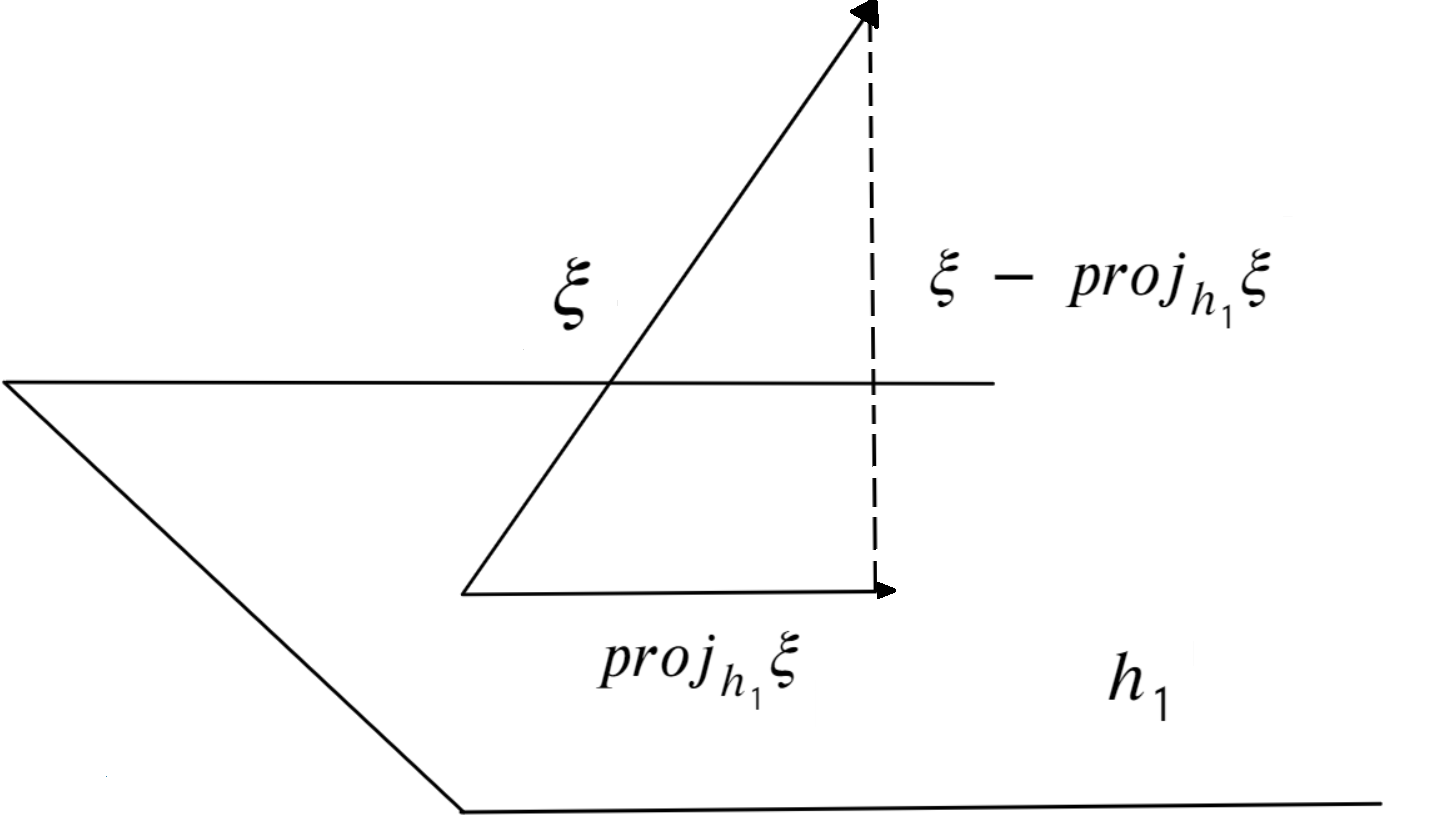
\includegraphics[scale=0.3]{lec7im1}
    \end{center}
  \end{itemize}

  Действительно, $ \displaystyle proj_{h_1}\xi = \sum\limits_{i = 1}^pb_ie_i$. Также $\displaystyle (\xi - proj_{h_1}\xi^Te_j = 0)$ для $ j = 1, \ldots, p $, $ \xi^Te_j = b_j = \eta_j$, тогда $(3)$ верно. Аналогично получаем:
  $$proj_{h_2}\xi = \sum\limits_{i = p + 1}^{p + m}\eta_ie_i \eqno(4)$$ 

  Если $ \eta = (\eta_1, \ldots, \eta_n)^T = (e_1^T, \ldots, e_n^T)^T\xi $, то $ (e_1^T, \ldots, e_n^T)^T $ -- ортонормированная матрица. В силу пункта $1)$ этой леммы $ \eta \sim N(0, \sigma^2E_n) $. По $(3)$, $(4)$ $ proj_{h_1}\xi $ и $ proj_{h_2}\xi $ независимы, так как определяются $ \eta_1, \ldots, \eta_p $ и $ \eta_{p + 1}, \ldots, \eta_{p + m} $ соответственно.

  Очевидно, что $ \lbrace proj_{h_i}\xi \rbrace, \; i = 1, 2$ -- гауссовские векторы, т.е. получаются линейным преобразованием гауссовского вектора $ \eta $. Например: 
  $$ proj_{h_1}\xi =  \underbrace{(e_1, \ldots, e_p)}_{\text{матрица }(n \times p )}(\eta_1, \ldots, \eta_p)^T$$ 
  Так же очевидно, что $ E \; proj_{h_1}\xi = 0 $, т.к. $ E\eta = 0 $. Наконец:
  $$\dfrac{1}{\sigma^2}|proj_{h_1}\xi|^2 = \dfrac{1}{\sigma^2} \left| \sum\limits_{i = 1}^p \eta_ie_i\right|^2 = \dfrac{1}{\sigma^2} \sum\limits_{i = 1}^p\eta_i^2 = \sum\limits_{i = 1}^p \left(\dfrac{\eta_i}{\sigma}\right)^2 \sim \chi^2(p = dim\left(h_1)\right)$$
\end{Proof}










\section{Линейная Гауссовская модель.}

$ X \sim N(l, \sigma^2E_n), \; \sigma^2 > 0, \sigma^2 $ -- неизвестно, $ l \in h $ -- неизвестно. $ h $ -- известное линейное подпространство $ \mathbb{R}^n, \; dimh = p < n. $ Если $ \varepsilon := x - l  $, то: 
$$X = l + \varepsilon, \; \varepsilon \sim N(0, \sigma^2E_n), l \in h\eqno(5)$$ 
Неизвестный параметр $ \theta \in \mathbb{R}^{n + 1}, \theta^T = (l^T, \sigma
^2)$. Пусть $ h^{\bot} $ -- ортогональное дополнение к $ h $ в $ \mathbb{R}^n $, то есть множество векторов из $ \mathbb{R}^n,  $ перпендикулярных $ h $. Тогда $ dim(h^{\bot}) = n - p $, и имеем:
$$ \forall x \in \mathbb{R}^n \; x = proj_hx + proj_{h^{\bot}} \eqno(6)$$

Найдем достаточную статистику для $ \theta $. Плотность $ X $ засчет $(5)$, $(6)$ есть 
$$ \begin{gathered}
  p(x, l, \sigma^2) = (\dfrac{1}{\sqrt{2 \pi}\sigma})^ne^{-\frac{1}{2\sigma^2}|x-l|^2}  \stackrel{\text{в силу} (6)}{=} (\dfrac{1}{\sqrt{2 \pi}\sigma})^n e^{-\frac{1}{2\sigma^2}|(proj_hx - l) + proj_{h^{\bot}}|^2} = \\
  = (\dfrac{1}{\sqrt{2 \pi}\sigma})^n e^{-\frac{1}{2\sigma^2}(|proj_hx - l|^2 + |proj_{h^{\bot}}|^2)} = \psi(T(x), \theta)h(x)
\end{gathered}$$ 
где $ T(x) = \left((proj_hx)^T, |proj_{h^{\bot}}|^2 \right)^T, h(x) = 1 $. В силу критерия факторизации $ T(x) $ -- достаточная статистика. Примем без доказательства, что это -- полная статистика.
 
\begin{itemize}
  \item[$1)$] 
    \colorbox{DarkSeaGreen}{Оптимальная оценка $ l $.} $ proj_hX = proj_hl = proj_h\varepsilon$, тогда $E\;proj_hX = l + E\;proj_h\varepsilon = l $ в силу пункта $2)$ леммы \ref{cha:7/lemma:1}. Итак, $ proj_hX $ есть функция полной достаточной статистики $ Eproj_hX = l $. По лемме \ref{cha:7/lemma:2} Лемана-Шеффе $ \hat{l^n} := proj_hX $ -- оптимальная оценка $ l $.
  \item[$2)$] 
    \colorbox{DarkSeaGreen}{Оптимаьная оценка $ \sigma^2 $}. $ proj_{h^{\bot}}X = proj_{h^{\bot}}l + proj_{h^{\bot}}\varepsilon = proj_{h^{\bot}}\varepsilon $. 

    В силу пункта $2)$ леммы \ref{cha:7/lemma:1} имеем:
    $$\dfrac{1}{\sigma^2}|proj_{h^{\bot}}X|^2 = \dfrac{1}{\sigma^2}|proj_{h^{\bot}}\varepsilon|^2 \sim \chi^2(n-p)\eqno(7)$$ 
    Значит, $ E\dfrac{1}{\sigma^2}|proj_{h^{\bot}}\varepsilon|^2 = n - p, \; E\dfrac{1}{n - p}|proj_{h^{\bot}}X|^2 = \sigma^2$. В силу леммы \ref{cha:7/lemma:2} Лемана-Шеффе $ \hat{s_n}^2 := \dfrac{1}{n - p}|proj_{h^{\bot}}X|^2 $ -- оптимальная оценка $ \sigma^2. $ Кроме того, по $(7)$ имеем:
    $$ \dfrac{(n - p)\hat{s_n}^2}{\sigma^2} = \dfrac{1}{\sigma^2}|proj_{h^{\bot}}X|^2 \sim \chi^2(n - p) \eqno(8)$$
  \item[$3)$] 
    \colorbox{DarkSeaGreen}{Независимость $ \hat{l_n} $ и $ \hat{s_n}^2 $}. В силу пункта $2)$ леммы \ref{cha:7/lemma:1} $ proj_hX = l + proj_h\varepsilon $ и $ proj_{h^{\bot}} X = proj_{h^{\bot}}\varepsilon  $ независимы, значит $\hat{l_n} \text{ и } \hat{s_n}^2 $ независимы.
\end{itemize}

В силу леммы \ref{cha:7/lemma:2} Лемана-Шеффе $ (\hat{l_n}^T, \hat{s_n}^2)^T $ -- оптимальная оценка вектора $ \theta = (l^T, \sigma^2)^T$. 
$$ \hat{l_n} = proj_hX = \underset{Y \in h}{argmin}|X-Y| = \underset{Y \in h}{argmin}|X-Y|^2 = \underset{Y \in h}{argmin}\sum\limits_{i = 1}^n(X_i - Y_i)^2$$
Поэтому $ \hat{l_n} $ и $ \hat{s_n}^2 = \dfrac{1}{n - p}|X - proj_hX|^2 $ называются \red{оценками по методу наименьших квадратов}. 
\begin{center}
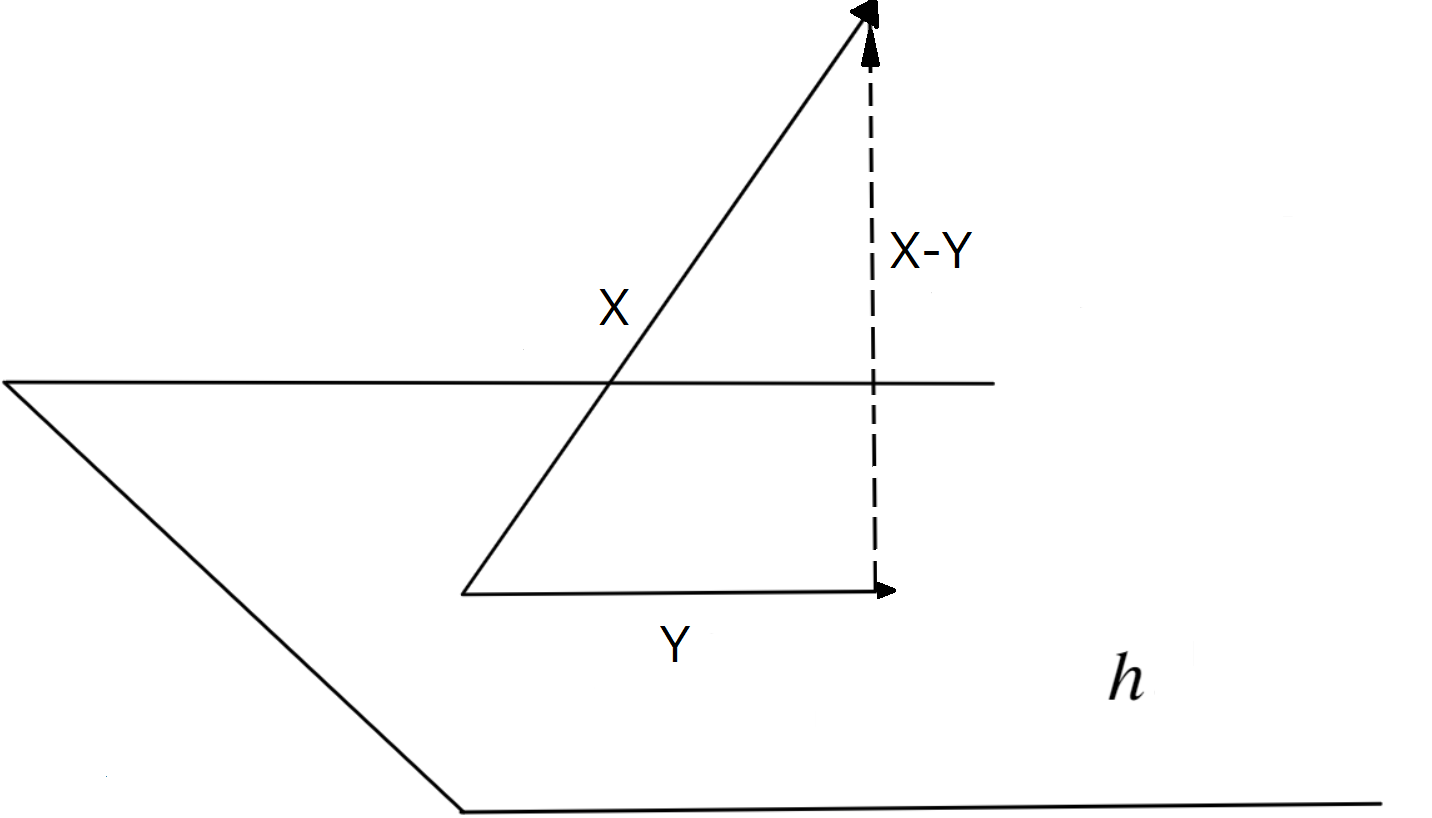
\includegraphics[scale=0.3]{lec7im2}
\end{center}

Выберем в $ h $ базис, пусть столбцы матрицы размера $ (n \times p)$  $Z = \{z_{ij}\}$, $i = 1, \dots, n, j = 1, \ldots, p $ будут базисными векторами. Тогда для некоторого $ c = (c_1, \ldots, c_p)^T $ имеем $ l = Zc $, и линейная модель (5) получает вид:
$$ X = Zc + \varepsilon\eqno(9)$$ 

Если $ z_i^T $ -- строки матрицы $ Z $, то (9) эквивалентно:
$$ X_i = z_i^Tc + \varepsilon_i, \; i = 1, \ldots, n \eqno(10)$$ 

Соотношения (9) и (10) задают \red{гауссовскую линейную регрессию}, это -- еще одна форма записи линейной модели (5).

В (9) неизвестный параметр $ \theta, \; \theta^T = (c^T, \sigma^2), dim(\theta) = p + 1 $. Матрица $ Z $ -- \red{регрессионная матрица}, она известна. $ X $ -- наблюдение. \textit{Надо оценить $ \theta, $} то есть $ \sigma^2. $

\begin{definition}
\red{Оценкой наименьших квадратов (н.к.) $ \hat{c_n} $ вектора $ c $} называется решение задачи $ |X - Z\alpha|^2 = \sum\limits_{i = 1}^n(X_i - z_i^T\alpha)^2 \longrightarrow \underset{\alpha \in \mathbb{R}^p}{min} $, то есть $ \hat{c_n} = \underset{\alpha \in \mathbb{R}^p}{argmin}|X-Z\alpha|$. 
\end{definition}

Пусть $ h $ -- линейное пространство столбцов Z, то есть столбцы Z -- базисные векторы h. Ясно, что $ |X - Z\alpha|^2 $ достигает минимума при $ \alpha = \hat{c_n} $ таком, что $ X-Z\hat{c_n} \bot h $, то есть $ Z^T(X - Z\hat{c_n}) = 0, \; Z^TX = Z^TZ\hat{c_n}$, тогда получаем:
$$\hat{c_n} = (Z^TZ)^{-1}Z^TX \eqno(11)$$
\begin{center}
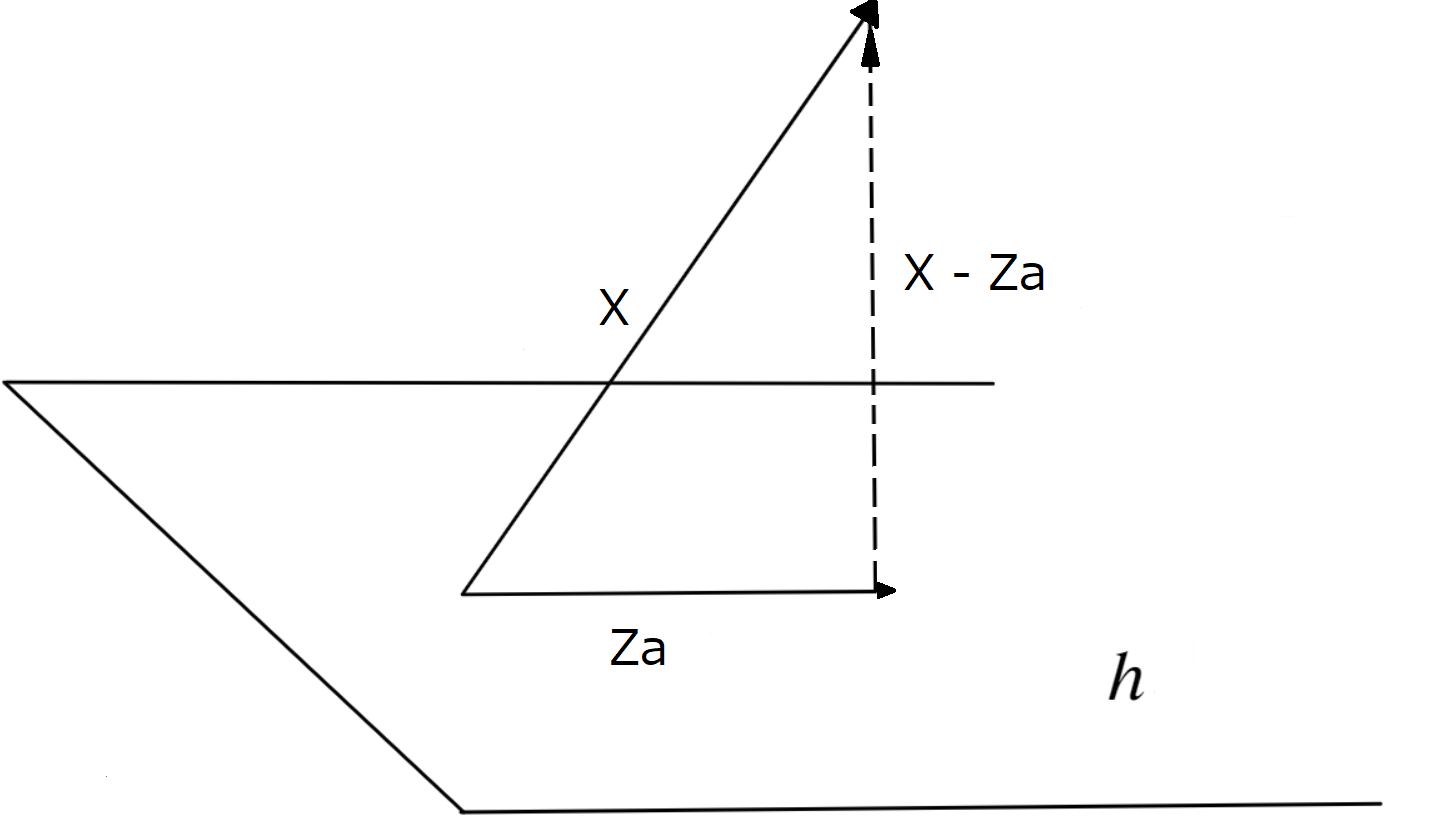
\includegraphics[scale=0.3]{lec7im3}
\end{center}

\textit{Отметим еще раз: $ Z\hat{c_n} = proj_hX $}. Матрица $ Z^TZ $ в (11) невырождена, так как при $ \alpha \neq 0 \; \alpha^TZ^TZ\alpha = |Z\alpha|^2 > 0$ из-за независимости столбцов Z.

\colorbox{DarkSeaGreen}{Оценка н.к. для $ \sigma^2 $}: $ \hat{s_n}^2 = \dfrac{1}{n - p}|X-Z\hat{c_n}|^2 $. Разумеется: 
$$ \displaystyle \hat{s_n}^2 = \dfrac{1}{n - p}\sum\limits_{i = 1}^n(x_i - z_i^T\hat{c_n})^2, \; \hat{s_n}^2 = \dfrac{1}{n-p}|proj_{h^{\bot}}X|^2 $$

\begin{definition}
  Вектор $ X - Z\hat{c_n} = (\hat{\varepsilon_1}, \ldots, \hat{\varepsilon_n})^T $  называют \red{вектором остатков}, а $ \hat{s_n}^2 $ -- \red{остаточной дисперсией.}
\end{definition}

\begin{theorem}\label{cha:8/the:1}
  Имеем несколько утверждений:
  \begin{itemize}
    \item[$1)$] 
      $ \hat{c_n}  \sim N(c, \sigma^2(Z^TZ)^{-1}), \; \dfrac{(n - p)\hat{s_n}^2}{\sigma^2} \sim \chi^2(n - p), \; E_{c, \sigma^2}\hat{s_n}^2 = \sigma^2, \; D_{c, \sigma^2}\hat{s_n}^2 = \dfrac{2\sigma^4}{n - p} $.
    \item[$2)$] 
      $ \hat{c_n} $ и $ \hat{s_n}^2 $ независимы. 
    \item[$3)$] 
      Оценки $ \hat{c_n} $ и $ \hat{s_n}^2 $ -- оптимальные оценки $ c $ и $ \sigma^2 $ соответственно.
  \end{itemize}
\end{theorem}
\begin{Proof}
  \begin{itemize}
    \item[$1)$] 
      \colorbox{DarkSeaGreen}{Распределение $ \hat{c_n} $}. В силу (11) $ \hat{c_n} $ есть линейное преобразование гауссовского вектора Х. В силу свойства 4 для гауссовких векторов, $ \hat{c_n} $ -- гауссовский вектор. 
      $$ E_{c, \sigma^2}\hat{c_n} = E_{c, \sigma^2}(Z^TZ)^{-1}Z^TX = (Z^TZ)^{-1}Z^TE_{c, \sigma^2}X = (Z^TZ)^{-1}Z^TZc = c $$
      То есть $ \hat{c_n} $ -- несмещенная оценка. 
      $$\begin{gathered}
        D_{c, \sigma^2}\hat{c_n} = E_{c, \sigma^2}(\hat{c_n} - c)(\hat{c_n} - c)^T = E_{c, \sigma^2}(Z^TZ)^{-1}Z^T(\varepsilon\varepsilon^T)Z(Z^TZ)^{-1} = \\
        = (Z^TZ)^{-1}Z^T(\sigma^2E_n)Z(Z^TZ)^{-1} = \sigma^2 (Z^TZ)^{-1}
      \end{gathered}$$
      Итак, $ \hat{c_n} \sim N(0, \sigma^2(Z^TZ)^{-1}) $.

      \colorbox{DarkSeaGreen}{Распределение $ \hat{s_n}^2 $}. Модель (9) эквивалентна $ X = l + \varepsilon $, где $ l = Zc, \; l \in h, \; h  \text{ -- пространство столбцов Z} $. В силу (13) и (8) $ \dfrac{(n-p)\hat{s_n}^2}{\sigma^2} \sim \chi^2(n - p ) $. Значит, $ E_{c, \sigma^2}\hat{s_n}^2 = \dfrac{\sigma^2}{n - p}\eta_{n - p} = \sigma^2 $. То есть $ \hat{s_n}^2 $ -- несмещенная оценка $ \sigma^2. $
    \item[$2)$] 
      В силу $(12)$ имеем:
      $$\hat{c_n} = (Z^TZ)^{-1}Z^TZ\hat{c_n} = (Z^TZ)^{-1}Z^Tproj_hX \eqno(14)$$
      Т.к. $proj_hX $ и $ proj_{h^{\bot}}X $ независимы, то $ \hat{c_n} $ и $ \hat{s_n}^2 $ независимы.
    \item[$3)$] 
      Докажем оптимальность $ \hat{c_n} $, оптимальность $ \hat{s_n}^2 $ доказывается аналогично. 

      Уже имеем, что $ \hat{c_n} $ -- несмещенная. Надо доказать, что: 
      $$ D_{c, \sigma^2}\hat{c_n} = D_{l, \sigma^2} \widehat{c_n} \; \forall l, \; \sigma^2 > 0\eqno(15)$$ 
      где $ \widehat{c_n} $ -- любая несмещенная оценка с. 

      У нас $ l = Zc, $ то есть $ Z^Tl = Z^TZc, \; c = (Z^TZ)^{-1}Z^Tl $. Имеем взаимно однознаное отображение $ c \longleftrightarrow l, \; l \in h, \; c \in \mathbb{R}^p $. Иогда левая часть (15) в силу (14) равна $ \displaystyle D_{c, \sigma^2}(Z^TZ)^{-1}Z^Tproj_hX $ -- ковариация функции полной достаточной статистики $ \left((proj_hx)^T, |proj_{h^{\bot}}|^2\right)^T $ для параметра $ (l^T, \sigma^2)^T $. Правая часть (15) есть $ E_{l, \sigma^2}\widehat{c_n} $. В силу леммы \ref{cha:7/lemma:2} Лемана-Шеффе $ \displaystyle D_{l, \sigma^2}(Z^TZ)^{-1}Zproj_hX \leq  D_{l, \sigma^2}\widehat{c_n} \; \forall l \in h, \; \sigma^2.$ Значит, (15) -- верно.
  \end{itemize}
\end{Proof}


\section{Пример(Гауссовская выборка.)}

\begin{example}
  Пусть $ X = (X_1, \ldots, X_n)^T $, где $ \lbrace X_i \rbrace $ -- н.о.р., $ X_1 \sim N(a, \sigma^2) $. Построим оптимальные оценки $ a $ и $ \sigma^2 $, исследуем их свойства.

  Пусть $ \varepsilon_i = X_i - a, \; i = 1, \ldots, n. $ Тогда:
  $$ X_i = a + \varepsilon_i, \; i = 1, \ldots, n; \; \lbrace \varepsilon_i \rbrace \text{ -- н.о.р., } \varepsilon_1 \sim N(0, \sigma^2) \eqno(16)$$

  Уравнение (16) -- частный случай линейной регрессии (10), где $ z_i^T = 1, \; c = a, \; p = 1. $ Значит, оптимальная оценка для $ a $ -- о.н.к., которая получается решением задачи $ \sum\limits_{i = 1}^n(X_i - \alpha)^2 \longrightarrow \underset{\alpha}{min} $. Эта задача эквивалентна решениюуравнения $ -2\sum\limits_{i = 1}^n(X_i - \alpha) = 0,$ корень -- $ \hat{\alpha_n} = \bar{X} $. 

  Оптимальная оценка для $ \sigma^2 $ -- остаточная дисперсия: $ \hat{s_n}^2 = \dfrac{1}{n - 1}\sum\limits_{i = 1}^n(X_i - \bar{X})^2 = S^2.$ Матрица $ Z = (z_1^T, \ldots, z_n^T)^T = (1, \ldots, 1)$, линейное пространство столбцов матрицы Z -- линейное пространство, натянутое на вектор $ (1, \ldots, 1)^T, \; l = (a_1, \ldots, a_n)^T $, оптимальная оценка $ l $ -- $ \hat{l} = Z\hat{c_n} = (\bar{X}, \ldots, \bar{X})^T $. Из теоремы \ref{cha:8/the:1} $ \bar{X} \sim N(a, \dfrac{\sigma^2}{n}), \; \dfrac{(n - 1)S^2}{\sigma^2} \sim \chi^2(n - 1). $

  $ \bar{X} $ и $ S^2 $ независимы. $ D_{a, \sigma^2}S^2 = \dfrac{2\sigma^2}{n - 1}. $ Ковариационная матрица вектора $ \hat{\theta_n} = (\bar{X}, S^2)^T $ есть $\displaystyle D_{a, \sigma^2}\hat{\theta_n} = 
  \begin{pmatrix}
    \dfrac{\sigma^2}{n}& 0\\
    0 & \dfrac{2\sigma^2}{n - 1}
  \end{pmatrix}$. Напомним, \red{матрица информации Фишера} (смотри раздел 5) равна $\displaystyle I(\theta) = 
  \begin{pmatrix}
    \dfrac{n}{\sigma^2}& 0\\
    0 & \dfrac{n}{2\sigma^2}
  \end{pmatrix}$, поэтому:
  $$D_{a, \sigma^2}\hat{\theta_n} = 
  \begin{pmatrix}
    \dfrac{\sigma^2}{n}& 0\\
    0 & \dfrac{2\sigma^2}{n - 1}
  \end{pmatrix} > I^{-1}(\theta) = 
  \begin{pmatrix}
    \dfrac{\sigma^2}{n}& 0\\
    0 & \dfrac{2\sigma^2}{n}
  \end{pmatrix}$$

  \textit{Значит, оценка $ (\bar{X}, S^2)^T $ является оптимальной оценкой $ (a, \sigma^2)^T $, но не является эффективной в $ C_{\mathbb{R}} $.}
\end{example}

\vspace{2cm}
\begin{definition}\label{cha:8/def:1}
  Пусть $ \xi_0, \ldots, \xi_k $ -- н.о.р. $ N(0, 1) $ сл.в. Случайная величина 
  $$\displaystyle t_k = \dfrac{\xi_0}{\sqrt{\dfrac{1}{k}(\xi_1^1 + \ldots + \xi_k^2)}} $$ 
  имеет \red{распределение Стьюдента с k степенями свободы}.
\end{definition}
То есть $ t_k = \dfrac{\xi_0}{\sqrt{\dfrac{1}{k}\eta_k}} $, где $ \xi_0 \sim N(0, 1), \; \eta_k \sim \chi^2(k), \; \xi_0 \text{ и } \eta_k $ независимы.\\

Поскольку $\displaystyle \dfrac{n^{\frac{1}{2}}(\bar{X - a})}{\sigma} \sim N(0, 1), \text{ а } \dfrac{(n - 1)S^2}{\sigma^2} \sim \chi^2(n - 1),  $ то: 
$$\displaystyle \dfrac{n^{\frac{1}{2}}(\bar{X - a})}{\sigma}\sqrt{\dfrac{1}{n-1}\dfrac{(n - 1)S^2}{\sigma^2}} = \dfrac{n^{\frac{1}{2}}(\bar{X} - a)}{S} \sim S(n - 1)$$

Величина $ \dfrac{n^{\frac{1}{2}}(\bar{X} - a)}{S} $ называется \red{стьюдентовой дробью}.













\chapter{Введение в доверительное оценивание} 

Пусть наблюдение $ X = (X_1, \ldots, X_n), \; X \sim P_{\theta}, \; \theta \in \Theta \in \mathbb{R}^1, \; \Theta $ -- интервал. Пусть $ T_1(X) \leq T_2(X), \; (T_1(X), T_2(X)) \subseteq \Theta $.

\begin{definition}
	Если $ P_{\theta}(T_1(X) < \theta < T_2(X)) \geq 1 - \alpha \;\; \forall \theta \in \Theta $, то случайный интервал $ (T_1(X), T_2(X)) $ называется \red{доверительным интервалом уровня $ 1 - \alpha $}, $ 0 < \alpha < 1 $.
\end{definition}

Интервал $ (T_1(X), T_2(X)) $ можно понимать как интервальную оценку (в отличие от точечной) параметра $ \theta $. Он покрывает неизвестное $ \theta $ с вероятностью, не меньшей, чем $ 1 - \alpha$.

\section{Доверительные интервалы для параметров Гауссовских выборок}

\subsection*{Доверительный интервал для среднего $ a $ при известной дисперсии $ \sigma^2 $}

$ X = (X_1, \ldots, X_n), \; \lbrace X_i \rbrace $ -- н.о.р., $ X_1 \sim N(a, \sigma^2) $.

Оптимальная оценка для $ a $ -- $ \bar{X} \sim N(a, \dfrac{\sigma^2}{n}) $. Значит, $ \dfrac{n^{\frac{1}{2}}(\bar{X} - a)}{\sigma} \sim N(0, 1) $. Пусть $ \phi(x) $ -- функция распределения $ N(0, 1) $, то есть $ \phi(x) = \dfrac{1}{\sqrt{2 \pi}} \int\limits_{- \inf}^x e^{-\frac{t^2}{2}}dt $. Пусть $ \xi_{\alpha}: \phi(\xi_{\alpha}) = \alpha, \; 0 < \alpha < 1 $.

Тогда $ \forall a \; P_a(|\dfrac{n^{\frac{1}{2}}(\bar{X} - a)}{\sigma}| < \xi_{1 - \frac{\alpha}{2}}) = 1 - \alpha, $ то есть с вероятностью $ 1 - \alpha$:
$$ -\xi_{1 - \frac{\alpha}{2}}< \dfrac{n^{\frac{1}{2}}(\bar{X} - a)}{\sigma} < \xi_{1 - \frac{\alpha}{2}}, \; \bar{X} - \dfrac{\sigma\xi_{1 - \frac{\alpha}{2}}}{\sqrt{n}} < a <  \bar{X} + \dfrac{\sigma\xi_{1 - \frac{\alpha}{2}}}{\sqrt{n}}$$

\begin{center}
	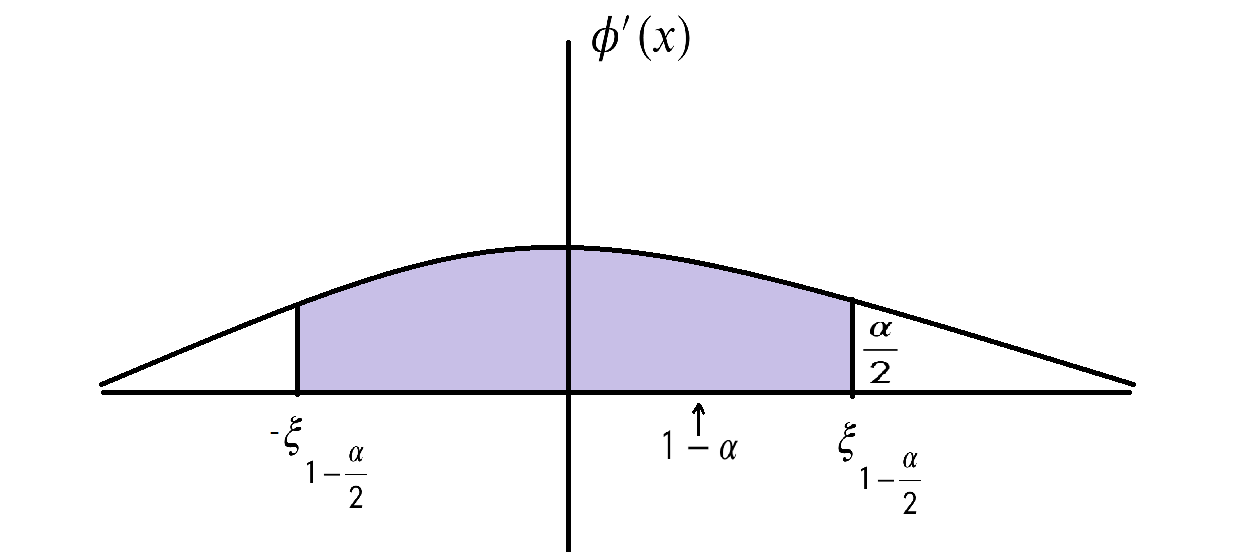
\includegraphics[scale=0.4]{N}

	$ \xi_{1 - \frac{\alpha}{2}} = -\xi_{\frac{\alpha}{2}} $
\end{center}

Интервал: 
$$ (\bar{X} - \dfrac{\sigma\xi_{1 - \frac{\alpha}{2}}}{\sqrt{n}}, \bar{X} + \dfrac{\sigma\xi_{1 - \frac{\alpha}{2}}}{\sqrt{n}}) \eqno(1)$$ 
называется \red{доверительным интервалом уровня $ 1 - \alpha $}, его длина $ ln = \dfrac{2\sigma\xi_{1 - \frac{\alpha}{2}}}{\sqrt{n}} $ю

\begin{property}
	Имеем несколько свойств:
	\begin{itemize}
		\item[$1)$] 
			$ \alpha \to 0 \; \Rightarrow \;  \xi_{1 - \frac{\alpha}{2}} \to \inf \; \Rightarrow \;  ln \to \inf $.
			\begin{remark}
				Обычно $ \alpha = 0.05, \; 0.01, \ldots $ и $ \alpha $ фиксировано.
			\end{remark}
		\item[$2)$] 
			$ n \to \inf \; \Rightarrow \;  ln \to 0 $.
		\item[$3)$] 
			$ \sigma \to 0 \; \Rightarrow \;  ln \to 0. $
	\end{itemize}
\end{property}

\begin{remark}
	Доверительных интервалов много. Например, $ \dfrac{X_1 - \theta}{\sigma} \sim N(0, 1) $, и на этой статистике можно построить доверительный интервал уровня $ 1 - \alpha $.
\end{remark}

\textit{Какой доверительный интервал наилучший?}

\begin{definition}
Доверительный интервал $ (T_1, T_2) $ уровня $ 1 - \alpha $ называется \red{несмещенным}, если $ P_{\theta}(T_1 < \theta' < T_2) \leq 1 - \alpha \; \forall \theta, \; \theta' $ таких, что $ \theta \neq \theta' $. То есть вероятность накрытия неверного параметра всегда \textbf{не больше} вероятности накрытия верного параметра.
\end{definition}

\begin{definition}
Несмещенный доверительный интервал $ (T_1, T_2) $ уровня $ 1 - \alpha $ называется \red{наиболее точным}, если он минимизирует вероятность $ P_{\theta}(T_1 < \theta' < T_2) \; \forall \theta, \; \theta' $ таких, что $ \theta \neq \theta' $ в классе всех \textbf{несмещенных} доверительных интервалов $ (T_1, T_2) $ уровня $ 1 - \alpha $.
\end{definition}

Можно показать, что (1) является наиболее точным несмещенным доверительным интервалом уровня $ 1 - \alpha $, то есть \textit{оптимальным}.

\subsection*{Доверительный интервал для среднего $ a $ при неизвестной дисперсии $ \sigma^2 $}
 
$ X = (X_1, \ldots, X_n), \; \lbrace X_i \rbrace $ -- н.о.р., $ X_1 \sim N(a, \sigma^2), \; n \geq 2 $.

\begin{definition}\label{cha:9/def:1}
	Если $ \xi_0, \ldots, \xi_k $ -- н.о.р. N(0, 1) сл.в., то сл.в. $$ \begin{gathered} t_k = \dfrac{\xi_0}{\sqrt{\dfrac{1}{k}(\xi_1^2 + \ldots + \xi_k^2)}} \end{gathered} $$ имеет \blue{распределение Стьюдента с к степенями свободы}. \textit{Обозначение:} $ t_k \sim S(k)$.
\end{definition}

Очевидно, $ t_k = \dfrac{\xi_0}{\sqrt{\frac{1}{k}\eta_k}}, \text{ где } \xi_0, \; \eta_k  $ независимы, $ \eta_k \sim \chi^2(k). $\\

Пусть $ S_k(x) := P(t_k \leq x) $ -- ф.р. $ t_k .$ Пусть $ S_k(t_{\alpha}(k)) = \alpha, \; 0 < \alpha < 1,  $ то есть $ t_{\alpha}(k) $ -- \red{квантиль уровня $ \alpha $ ф.р. $ S_k(x) $}. Поскольку $ t_k \stackrel{d}{t_k} $, то плотность вероятности $ S_k(x)' $ -- четная функция. Значит, $ -t_{\alpha}(x) = t_{1 - \alpha}(x) $.

Известно, что $ \bar{X} $ и $ s^2 $ -- оптимальные оценки $ a, \; \sigma^2 $, $ \bar{X} $ и $ s^2 $ независимы, 
$$ \begin{gathered} \dfrac{n^{\frac{1}{2}}(\bar{X} - a)}{\sigma} \sim N(0, 1), \; \dfrac{(n - 1)s^2}{\sigma^2} \sim \chi^2(n - 1) \end{gathered} $$ 
Здесь $ s^2 = \dfrac{1}{n -1}\sum\limits_{i = 1}^{n}(X_i - \bar{X}).  $ Значит: 
$$ \begin{gathered} \dfrac{n^{\frac{1}{2}}(\bar{X} - a)}{\sigma} / \sqrt{\dfrac{1}{n - 1} \dfrac{(n - 1)s^2}{\sigma^2}} = \dfrac{n^{\frac{1}{2}}(\bar{X} - a)}{s} \sim S(n - 1).  \end{gathered}$$
Значит: $$ \begin{gathered} P_{a, \sigma^2}(|\dfrac{n^{\frac{1}{2}}(\bar{X} - a)}{s}|) < t_{1 - \frac{\alpha}{2}}(n - 1) = 1 - \alpha. \end{gathered} $$ Получаем доверительный интервал уровня $ 1 - \alpha: $ $$ \begin{gathered} \bar{X} - \dfrac{st_{1 - \frac{\alpha}{2}}(n - 1)}{\sqrt{n}} < a < \bar{X} + \dfrac{st_{1 - \frac{\alpha}{2}}(n - 1)}{\sqrt{n}} \end{gathered} $$

\subsection*{Доверительный интервал для дисперсии $ \sigma^2 $ при неизвестном среднем $ a $}

$ X = (X_1, \ldots, X_n), \; \lbrace X_i \rbrace $ -- н.о.р., $ X_1 \sim N(a, \sigma^2), \; n \geq 2 $. 

Знаем, что $ \dfrac{(n - 1)s^2}{\sigma^2} \sim \chi^2(n - 1). $ Обозначим за $ \chi_{(n - 1)}(x) $ ф.р. $ \chi^2(n - 1), \; x_{\alpha}(n - 1) $ -- квантиль уровня $ \alpha, $ то есть $ \chi_{(n - 1)}(x_{\alpha}(n - 1)) = \alpha, \; 0 < \alpha < 1.$ Тогда $ P_{a, \sigma^2}(x_{\frac{\alpha}{2}}) < \dfrac{(n - 1)s^2}{\sigma^2} < x_{1 - \frac{\alpha}{2}}(n - 1)) = 1 - \alpha .$ Доверительный интервал уровня $ 1 - \alpha $: $$ \begin{gathered} \dfrac{(n - 1)s^2}{x_{1 - \frac{\alpha}{2}}(n - 1)} < \sigma^2 < \dfrac{(n - 1)s^2}{x_{\frac{\alpha}{2}}(n - 1)} \end{gathered} $$

\section{Оценивание параметров линейной регрессии}

Если $ \eta_k \sim \chi^2(k), \; \upsilon_m \sim \chi^2(m),  $ $ \eta_k $ и $ \upsilon_m $ независимы, то сл.в. $ f_{k, m} = \dfrac{\frac{1}{k}\eta_k}{\frac{1}{m}\upsilon_m} $ имеет распределение Фишера с $ (k, m) $ степенями свободы. Пишем $ f_{k, m} \sim F(k, m). $ Пусть $ F_{k, m}(x) $ -- ф.р., то есть $ F_{k, m}(f_{\alpha}(k, m)) = \alpha, \; 0 < \alpha < 1 $. 

\begin{lemma}\label{cha:9/lemma:1}
Если $ \xi \in \mathbb{R}^k, \; \xi \sim N(0, \Sigma), \; \Sigma > 0, $ то $ \sigma^T\Sigma^{-1}\sigma \sim \chi^2(k) $.
\end{lemma}
\begin{Proof}
	$$ \begin{gathered} \sigma^T\Sigma^{-1}\sigma = (\Sigma^{-\frac{1}{2}}\xi)^T(\Sigma^{-\frac{1}{2}}\xi) = |\Sigma^{-\frac{1}{2}}\xi|^2 \end{gathered} $$
	При этом $ \eta := \Sigma^{-\frac{1}{2}}\xi \sim N(0, E_k), $ так как $ \eta $ -- гаусс. Тогда: 
	$$ \begin{gathered} 
		E\eta = \Sigma^{-\frac{1}{2}}E\eta = 0, \; Cov(\eta, \eta) = E\eta\eta^T = \Sigma^{-\frac{1}{2}}\Sigma\Sigma^{-\frac{1}{2}} = E_k, \\
		\text{т.е. } |\Sigma^{-\frac{1}{2}}\xi|^2 = |\eta|^2 = \eta_1^1 + \ldots + \eta_k^2 \sim \chi^2(k)
	\end{gathered} $$
\end{Proof}

Рассмотрим регрессию $ X = Zc + \varepsilon, \; \varepsilon \sim N(0, \sigma^2E_n) $. Пусть $ \hat{c_n} $ -- о.н.к. для $ c, \; \hat{s_n}^2 $ -- о.н.к. для $ \sigma^2 $.

Тогда известно, $ \hat{c_n} \sim N(c, \sigma^2(Z^TZ)^{-1}), \dfrac{(n - p)\hat{s_n}}{\sigma^2} \sim \chi^2(n - p), $ $ \hat{c_n} $ и $ \hat{s_n}^2 $ независимы. Значит, в силу леммы \ref{cha:9/lemma:1}: 
$$ \begin{gathered} 
	\dfrac{1}{\sigma^2}(\hat{c_n} - c)^T(Z^TZ)(\hat{c_n} - c) \sim \chi^2(p), \\ f_{p, n - p} := \dfrac{\frac{1}{p}\frac{1}{\sigma^2}(\hat{c_n} - c)^T(Z^TZ)(\hat{c_n} - c)}{\frac{1}{n - p}\frac{(n - p)\hat{s_n}^2}{\sigma^2}} = \dfrac{(\hat{c_n} - c)^T(Z^TZ)(\hat{c_n} - c)}{p\hat{s_n}^2} \sim F(p, n - p)
\end{gathered} $$ 
Значит: 
$$ \begin{gathered} 
	P_{c, \sigma^2}((\hat{c_n} - c)^T(Z^TZ)(\hat{c_n} - c) \leq p\hat{s_n}^2f_{1 - \alpha}(p, n - p)) = 1 - \alpha 
\end{gathered} $$ 

\red{Доверительный эллипсоид уровня $ 1 - \alpha $}: 
$$ \begin{gathered} \lbrace c: \; (\hat{c_n} - c)^T(Z^TZ)(\hat{c_n} - c) < p\hat{s_n}^2f_{1 - \alpha}(p, n - p)\rbrace \end{gathered} $$ 
\textit{ Он накрывает неизвестный c с вероятностью $ 1 - \alpha $}.\\

Пусть $ c = (c_1, \ldots, c_p)^T, \; \hat{c_n} = (\hat{c_1}, \ldots, \hat{c_p})^T,  $ тогда $ \hat{c_{in}} \sim N(c_i, \sigma^2a_{ii}),  $ где $ (Z^TZ)^{-1} = (a_{ij}), \; i,j = 1, \ldots, p. $ Так как $ \hat{c_{in}} $ и $ \hat{s_n}^2$ независимы, то $$ t_{n - p}:= \dfrac{\hat{c_{in}} - c_i}{\sqrt{\sigma^2a_{ii}}} / \sqrt{\dfrac{1}{n - p}\dfrac{(n - p)\hat{s_n}^2}{\sigma^2}} = \dfrac{\hat{c_{in}} - c_i}{\hat{s_n}\sqrt{a_{ii}}} \sim S(n - p). $$

Доверительный интервал для $ c_i $ уровня $ 1 - \alpha :$ $$ \begin{gathered} \hat{c_{in}} - \hat{s_n}\sqrt{a_{ii}}t_{1 - \frac{\alpha}{2}}(n - p) < c_i < \hat{c_{in}} + \hat{s_n}\sqrt{a_{ii}}t_{1 - \frac{\alpha}{2}}(n - p) \end{gathered} $$.

\section{Ассимптотический доверительный интервал}

Пусть для неизвестного параметра $ \theta \in \Theta \in \mathbb{R}^1  $ существует ассимптотически нормальная оценка $ \hat{\theta_n} $, то есть:
$$n^{\frac{1}{2}}(\hat{\theta_n} - \theta) \stackrel{d}{\longrightarrow} N(0, \sigma^2(\theta)), \; n \to \inf \eqno(2)$$.

Предположим, что $ \sigma^2(\theta) > 0 \; \forall \theta \in \Theta$ и $ \sigma^2(\theta) $ непрерывна по $ \theta $. В силу (2) $ \hat{\theta_n} - \theta = n^{-\frac{1}{2}}n^{\frac{1}{2}}(\hat{\theta_n} - \theta) \stackrel{P}{\to} 0, \; n \to \inf, $ то есть $ \hat{\theta_n} $ -- состоятельная оценка $ \theta $. Значит: 
$$ \hat{\sigma_n}^2 := \sigma^2(\theta), \; n \to \inf \eqno(3)$$
В силу (2), (3) $ \dfrac{n^{\frac{1}{2}}(\hat{\theta_n} - \theta)}{\hat{\sigma_n}} \stackrel{d}{\to} N(0, 1), \; n \to \inf $. Значит, $ \displaystyle P_{\theta}(|\dfrac{n^{\frac{1}{2}}(\hat{\theta_n} - \theta)}{\hat{\theta_n}}| < \xi_{1 - \frac{\alpha}{2}}) \to 1 - \alpha, \; n \to \inf $.

Ассимптотический доверительный интервал уровня $ 1 - \alpha $ имеет вид: 
$$ \hat{\theta_n} - \dfrac{\hat{\sigma_n}\xi_{1 - \frac{\alpha}{2}}}{\sqrt{n}} < \theta <  \hat{\theta_n} + \dfrac{\hat{\sigma_n}\xi_{1 - \frac{\alpha}{2}}}{\sqrt{n}} $$ 
Он накрывает неизвестный параметр $ \theta $ прмерно с вероятностью $ 1 - \alpha $ при больших $ n $.

\section{Примеры}

\begin{example}
$ X = (X_1, \ldots, X_n), \; \lbrace X_i \rbrace $ -- н.о.р., $ X_1 \sim Pois(\theta), \; \theta > 0 $. Тогда $\displaystyle  n^{\frac{1}{2}}(\bar{X} - \theta) \stackrel{d}{\longrightarrow} N(0, \theta),  $ а т.к. $ \bar{X} \stackrel{P}{\longrightarrow} \theta,$ то $ \dfrac{n^{\frac{1}{2}}(\bar{X} - \theta)}{\sqrt{\bar{X}}} \stackrel{d}{\longrightarrow} N(0, 1) $. Ассимптотический доверительный интервал уровня $ 1- \alpha $: 
$$ \bar{X} - \dfrac{\sqrt{\bar{X}}\xi_{1 - \frac{\alpha}{2}}}{\sqrt{n}} < \theta <  \bar{X} + \dfrac{\sqrt{\bar{X}}\xi_{1 - \frac{\alpha}{2}}}{\sqrt{n}}$$
\end{example}

\begin{example}
$ X_1 \sim R(0, \theta), \; \theta > 0 $. 
$$ E_{\theta}X_1 = \dfrac{\theta}{2}, \; D_{\theta}X_1 = \dfrac{\theta^2}{12}, \; 2\bar{X} \stackrel{P}{\to} \theta, \; \dfrac{n^{\frac{1}{2}}(\bar{X}-\frac{\theta}{2})}{\frac{\theta}{2}\sqrt{3}} \stackrel{d}{\to} N(0, 1), \; n \to \inf$$ 
Значит: 
$$ \dfrac{\sqrt{3n}(2\bar{X} - \theta)}{\theta} \stackrel{d}{\to} N(0, 1), \; \dfrac{\sqrt{3n}(2\bar{X} - \theta)}{2\bar{X}} \stackrel{d}{\to} N(0, 1)$$

Ассимптотический доверительный интервал:
$$ 2\bar{X} - \dfrac{2\bar{X}\xi_{1 - \frac{\alpha}{2}}}{\sqrt{3n}} < \theta <  2\bar{X} + \dfrac{2\bar{X}\xi_{1 - \frac{\alpha}{2}}}{\sqrt{3n}}$$
\end{example}




































\chapter{Ассимптотически оптимальные оценки.}

\section{Сходимости, лемма Слуцкого} %\label{lec:1/sec:1}

Пусть случайные величины $\xi_n, \xi \in \mathbb{R}^n$ определены на колмогоровой тройке $(\Omega, F, P)$.
$F_n (x)$ - функция распределения $\xi_n$, $\varphi_n (t)$ - характеристическая функция, $Q_n$ - распределение (мера на множестве борелевских подмножеств).

\begin{definition}\label{lec:1/def:1}
	Говорят, что $F_n$ сходится к $F$ \red{в основном} ($F_n(x) \Rightarrow F(x)$), если $F_n(x) \to F(x) \; \forall x \in \mathbb{C}(F)$.
\end{definition}

\begin{definition}\label{lec:1/def:2}
	Говорят, что $Q_n$ сходится \red{слабо} к $Q$ ($Q_n \xrightarrow[]{W} Q$), если для любой непрерывной и ограниченной функции $g: \mathbb{R}^k \to \mathbb{R}^1$
	$$\underset{\mathbb{R}^k}{\overset{}{\int}}g(x) Q_n(dx) \to \underset{\mathbb{R}^1}{\overset{}{\int}}g(x) Q(dx) \; \Leftrightarrow \; E g(\xi_n) \to E g(\xi)$$ 
\end{definition}

\begin{theorem}[]\label{lec:1/the:1}
	Следующие условия эквивалентны:
	\begin{enumerate}
		\item $F_n \Rightarrow F$
		\item $Q_n \xrightarrow[]{W} Q$
		\item $\varphi_n (t) \to \varphi (t) \; \forall t \in \mathbb{R}^k$
	\end{enumerate}
\end{theorem}

\begin{definition}\label{lec:1/def:3}
	Если выполнено одно из условий $1)-3)$ из предыдущей теоремы, то говорят, что $\xi_n$ сходится к $\xi$ \red{по распределению} ($\xi_n \xrightarrow[]{d}\xi$). 
\end{definition}

\begin{theorem}[\blue{о наследовании сходимости}]\label{lec:1/the:2}
	Пусть $\xi_n, \xi \in \mathbb{R}^k$ и отображение $H: \mathbb{R}^k \to \mathbb{R}^1$ непрерывно. Тогда:
	\begin{enumerate}
		\item если $\xi_n \xrightarrow[]{d} \xi$, то $H(\xi_n) \xrightarrow[]{d} H(\xi)$
		\item если $\xi_n \xrightarrow[]{P} \xi$, то $H(\xi_n) \xrightarrow[]{P} H(\xi)$
	\end{enumerate}
\end{theorem}

\newpage
\begin{lemma}[\blue{Слуцкого}]\label{lec:1/lemma:1}
	Пусть $\xi_n, \xi, \eta_n, a \in \mathbb{R}^1$ и $\xi_n \xrightarrow[]{d}\xi, \eta_n \xrightarrow[]{P} a$. Тогда:
	\begin{itemize}
		\item[$\RNumb{1})$] $\xi_n + \eta_n \xrightarrow[]{d} \xi + a$
		\item[$\RNumb{2})$] $\xi_n \eta_n \xrightarrow[]{d} a \xi$
	\end{itemize}
\end{lemma}
\begin{Proof}
	Достаточно, чтобы была следующая сходимость:
	$$(\xi_n, \eta_n)^T \xrightarrow[]{d} (\xi, a)^T\eqno(1)$$
	Действительно, если $(1)$ верно, то при $H(x,y) = x+y$ по теореме $1.2$ получаем $\RNumb{1}$, а при $H(x,y) = xy$ получаем $\RNumb{2}$.

	Докажем $(1): \; (\xi_n, \eta_n)^T \xrightarrow[]{d}(\xi, a)^T$. Проверим, что характеристическая функция $(\xi_n, \eta_n)^T$ сходится к характеристической функции $(\xi, a)^T$:
	$$|E e^{i t \xi_n + i s \eta_n} - E e^{i t \xi + i s a}| \le |E e^{i t \xi_n + i s \eta_n} - E e^{i t \xi_n + i s a}| + |E e^{i t \xi_n + i s a} - E e^{i t \xi + i s a}| = \alpha_n + \beta_n$$
	$$\begin{gathered}
	\alpha_n \le E|e^{i t \xi_n} (e^{i s \eta_n} - e^{i s a})| = E|e^{i s \eta_n} - e^{i s a}| = E g(\eta_n) \\ 
	g(x) = |e^{i s x} - e^{i s a}| \text{ - непрерывная и ограниченная}, \; \eta_n \xrightarrow[]{d} a \; \Rightarrow \\
	\text{по теореме } 1.2 \;\; E g(\eta_n) \to E g(a) = 0 \; \Rightarrow \; \alpha_n \to 0
	\end{gathered}$$
	$$\begin{gathered}
		\beta_n = |E e^{i s a} (e^{i t \xi_n} - e^{i t \xi})| = |e^{i s a} E (e^{i t \xi_n} - e^{i t \xi})| = |E e^{i t \xi_n} - E e^{i t \xi}| \to 0, \text{ т.к. } \xi_n \xrightarrow[]{d}\xi.
	\end{gathered}$$

	Т.о. $\varphi_n (t) \to \varphi (t)$.
\end{Proof}

\section{Асимптотически нормальные, состоятельные оценки, асимптотический доверительный интервал}\label{lec:1/sec:2}

Пусть наблюдение $X \sim P_{\theta}, \; \theta \in \Theta \subseteq \mathbb{R}^k$. $\hat{\theta_n}$ - оценка $\theta$.

\begin{definition}\label{lec:1/def:4}
	Если $\sqrt{n} (\hat{\theta_n} - \theta) \xrightarrow[]{d} N(0, \Sigma (\theta)) \; \forall \theta \in \Theta$ и $0 < \Sigma (\theta) < \infty$, то $\hat{\theta_n}$ называется \red{асимптотически нормальной оценкой}.
\end{definition}

\begin{definition}\label{lec:1/def:5}
	Если $\hat{\theta_n} \xrightarrow[]{P} \theta \; \forall \theta \in \Theta$, то $\hat{\theta_n}$ называется \red{состоятельной оценкой}.
\end{definition}

Пусть $\theta \in \Theta \subseteq \mathbb{R}^1$, т.е. $\theta$ и $\hat{\theta_n}$ - скаляры.\\

Если $\hat{\theta_n}$ - состоятельная оценка $\theta$, то при больших $n$ $\hat{\theta_n} \simeq \theta$ с вероятностью, близкой к единице.\\

Если $\hat{\theta_n}$ - асимптотически нормальная оценка $\theta$, то есть $\sqrt{n} (\hat{\theta_n} - \theta) \xrightarrow[]{d} N(0, \sigma^2 (\theta)), \; 0 < \sigma^2 (\theta) < \infty \; \forall \theta \in \Theta$, то:
\begin{enumerate}
	\item $\hat{\theta_n}$ - состоятельная оценка $\theta$, т.к. $\hat{\theta_n} - \theta = \frac{1}{\sqrt{n}} \sqrt{n} (\hat{\theta_n} - \theta) \xrightarrow[]{P}0$ в силу пункта $\RNumb{2}$ леммы Слуцкого.
	\item скорость сходимости $\hat{\theta_n}$ к $\theta$ есть $\mathcal{O}(\sqrt{n})$
	\item при больших $n$ случайную величину $\sqrt{n}(\hat{\theta_n} - \theta)$ можно рассматривать как гауссовскую величину.
	\begin{example}\label{lec:1/example:1}
	Пусть $\sigma^2 (\theta)$ - непрерывная функция, а $\theta$ неизвестно. Тогда:
	$$\begin{gathered}
		\frac{\sqrt{n} (\hat{\theta_n} - \theta)}{\sigma (\hat{\theta_n})} = \frac{\sqrt{n} (\hat{\theta_n} - \theta)}{\sigma (\theta)} \cdot \frac{\sigma (\theta)}{\sigma (\hat{\theta_n})}\\
		\frac{\sqrt{n} (\hat{\theta_n} - \theta)}{\sigma (\theta)} \xrightarrow[]{d} N(0,1), \; \frac{\sigma (\theta)}{\sigma (\hat{\theta_n})} \xrightarrow[]{P} 1 \; \Rightarrow \\
		\Rightarrow \; \frac{\sqrt{n} (\hat{\theta_n} - \theta)}{\sigma (\hat{\theta_n})} \xrightarrow[]{d} \eta \sim N(0,1) \text{ в силу пункта } \RNumb{2}) \text{ леммы Слуцкого.}\\
		\text{Значит: } P_{\theta}\left( |\frac{\sqrt{n} (\hat{\theta_n} - \theta)}{\sigma (\hat{\theta_n})}| < \xi_{1 - \frac{\alpha}{2}} \right) \to P(|\eta| < \xi_{1 - \frac{\alpha}{2}}) = 1 - \alpha \\
		\text{Т.е. примерно с вероятность $1-\alpha$ выполнено неравенство:}\\
		\hat{\theta_n} - \frac{1}{\sqrt{n}} \sigma (\hat{\theta_n}) \xi_{1 - \frac{\alpha}{2}} < \theta < \hat{\theta_n} + \frac{1}{\sqrt{n}} \sigma (\hat{\theta_n}) \xi_{1 - \frac{\alpha}{2}}\\
		\text{Это называется \red{асимптотическим доверительным интервалом}}\\
		\text{для $\theta$ уровня $1 - \alpha$}.
	\end{gathered}$$
	\end{example}
	\item асимтотические гауссовские оценки можно сравнивать между собой:

	если $\sqrt{n} (\hat{\theta_{in}} - \theta) \xrightarrow[]{d} N(0, \sigma_i^2 (\theta)) \; \forall i = 1, 2, \dots$, то можно определить \red{асимтотическую нормальную эффективность}:
	$$\begin{gathered}
		e_{1,2} = \frac{\sigma_2^2 (\theta)}{\sigma_1^2 (\theta)} \\
		\text{напоминание: } e_{1,2} = \underset{n\to \infty}{\lim} \frac{n' (n)}{n}, \text{где } \begin{cases}
			\sqrt{n} (\hat{\theta_{1n}} - \theta) \xrightarrow[]{d} N(0, \sigma_1^2 (\theta))\\
			\sqrt{n} (\hat{\theta_{2n'}} - \theta) \xrightarrow[]{d} N(0, \sigma_1^2 (\theta))
		\end{cases}
	\end{gathered}$$
\end{enumerate}

$$\text{Вопрос: существует ли }\theta_n^{*} \text{ такая, что } e_{\theta_n^{*}, \hat{\theta_n}} (\theta) \ge 1 \; \forall \hat{\theta_n} \; \forall \theta \in \Theta\text{ ?}$$
Если есть, то $\theta_n^{*}$ требует не больше наблюдений, чем любая $\hat{\theta_n}$, чтобы достичь одинаковой с $\hat{\theta_n}$ точности.\\

Предельная дисперсия $\sqrt{n}(\theta_n^{*} - \theta)$ должна быть не больше асимптотической дисперсии $\sqrt{n}(\hat{\theta_n} - \theta)$ для любой асимптотической гауссовской оценки $\hat{\theta_n}$.

\section{Теорема Бахадура, асимптотически эффективная оценка}\label{lec:2/sec:1}

\begin{theorem}[\red{Бахадура}]\label{lec:2/the:1}
	Пусть $X_1, \dots, X_n$ - н.о.р.с.в., $X_1$ имеет плотность вероятности $f(x, \theta), \theta \in \Theta \subseteq \mathbb{R}^1$ по мере $\nu$. Пусть выполнены условия:
	\begin{itemize}
		\item[$(i)$] $\theta$ - интервал
		\item[$(ii)$] носитель $N_f = \Set{x}{f(x,\theta) > 0}$ не зависит от $\theta$
		\item[$(iii)$] $\forall x \in N_f$ плотность $f(x, \theta)$ дважды непрерывно дифференцируема по $\theta$
		\item[$(iv)$] интеграл $\int f(x, \theta) \nu (dx)$ можно дважды дифференцировать по $\theta$, внося знак дифференцирования под знак интеграла
		\item[$(v)$] информация Фишера $0 < i(\theta) < \infty \; \forall \theta \in \Theta$
		\item[$(vi)$] $|\frac{\partial^2}{\partial \theta^2} \ln f(x,\theta)| \le M(x) \; \forall x \in N_f, \theta \in \Theta$ и $E_{\theta} M(X_1) < \infty$
	\end{itemize}
	Тогда если $\sqrt{n}(\hat{\theta_n} - \theta) \xrightarrow[]{d}N(0, \sigma^2(\theta))$, то $\sigma^2 (\theta) \ge \frac{1}{i(\theta)}$ всюду за исключением множества Лебеговой меры нуль.
\end{theorem}

\begin{remark}\label{lec:2/remark:1}
	Если вдобавок $\sigma^2 (\theta)$ и $i(\theta)$ непрерывны, то $\sigma^2 (\theta) \ge \frac{1}{i(\theta)} \; \forall \theta \in \Theta$.
\end{remark}

\begin{definition}\label{lec:2/def:1}
	Если $\theta, \hat{\theta_n} \in \mathbb{R}^1$ и $\sqrt{n} (\hat{\theta_n} - \theta) \xrightarrow[]{d} N(0, \frac{1}{i(\theta)}), n \to \infty, \forall \theta \in \Theta$, причем $0 < i(\theta) < \infty$, то $\hat{\theta_n}$ называется \red{асимтотически эффективной оценкой} (асимптотически оптимальной оценкой).
\end{definition}

\newpage
\section{Правдоподобие, экстремальное свойство правдоподобия}\label{lec:2/sec:2}

Пусть далее $X = (X_1, \dots, X_n), \; X \sim P_{\theta}, \theta \in \Theta \subseteq \mathbb{R}^1$.\\

\textbf{\blue{Условие (А)}}
\begin{itemize}
	\item[$(i)$] $\theta$ - интервал, $P_{\theta_1} \not = P_{\theta_2}$ при $\theta_1 \not = \theta_2$
	\item[$(ii)$] $X_1, \dots, X_n$ - н.о.р.с.в., $X_1$ имеет плотность вероятности $f(x, \theta)$ по мере $\nu$, носитель $N_f = \Set{x}{f(x, \theta) > 0}$ не зависит от $\theta$.
\end{itemize}

Плотность вектора $X$ есть $p(x, \theta) = \underset{i=1}{\overset{n}{\Pi}} f(x_i, \theta)$.

\begin{definition}\label{lec:2/def:2}
	Функция $p(x, \theta)$ как функция $\theta$ при фиксированном $x$ называется \red{правдоподобием}.
\end{definition}

\begin{definition}\label{lec:2/def:3}
	Функция $Ln (x, \theta) = \ln p(x, \theta) = \underset{i=1}{\overset{n}{\sum}}\ln f(x_i, \theta)$ называется \red{логарифмическим правдоподобием}.
\end{definition}

Пусть $\theta_0$ - истинное значение параметра.

\begin{theorem}[\blue{экстремальное свойство правдоподобия}]\label{lec:2/the:1}
	Пусть выполнено условие (А), пусть $E_{\theta_0} |\ln f(x_1, \theta)| < \infty \; \Rightarrow \; P_{\theta_0} (p(x, \theta_0) > p(x, \theta)) \xrightarrow[n \to \infty]{} 1$, когда $\theta_0 \not = \theta$.
\end{theorem}
\begin{Proof}
$$\begin{gathered}
	p(x, \theta_0) > p(x, \theta) \; \Leftrightarrow \; \ln p(x, \theta_0) > \ln p(x, \theta) \; \Leftrightarrow \\
	\Leftrightarrow \; \eta_n := \frac{1}{n} \underset{i=1}{\overset{n}{\sum}} \ln \left( \frac{f(x_i, \theta)}{f(x_i, \theta_0)} \right) < 0, \text{ где } \ln \left( \frac{f(x_i, \theta)}{f(x_i, \theta_0)} \right) \text{ - борелевские функции.}\\
	\text{Т.е. надо показать, что } P_{\theta_0} (\eta_n < 0) \to 1 \\
	\text{ но } \eta_n = \frac{1}{n} \underset{i=1}{\overset{n}{\sum}}\ln \left( \frac{f(x_i, \theta)}{f(x_i, \theta_0)} \right) \xrightarrow[]{P} E_{\theta} \ln \left( \frac{f(x_1, \theta)}{f(x_1, \theta_0)} \right) \\ 
	\text{ (в силу слабого ЗБЧ в форме Чебышева)}.
\end{gathered}$$
\blue{Неравенство Йенсена}: пусть $g(x)$ выпуклая снизу борелевская функция, $E|\xi| < \infty, \; E|g(\xi)| < \infty \; \Rightarrow \; g(E \xi) \le E g(\xi)$. Если $\xi$ не является почти наверно константой и $g$ строго выпукла, то неравенство строгое.\\

Функция $-\ln x$ строго выпукла и $\frac{f(x_1, \theta)}{f(x_1, \theta_0)}$ не является почти наверно константой в силу пункта $(i)$ условия (А). Тогда в силу неравенства Йенсена получаем:
$$\begin{gathered}
	E_{\theta_0} \ln \frac{f(x_1, \theta)}{f(x_1, \theta_0)} < \ln E_{\theta_0} \frac{f(x_1, \theta)}{f(x_1, \theta_0)} = \\
	= \ln \underset{N_f}{\overset{}{\int}}\frac{f(x, \theta)}{f(x, \theta_0)} f(x, \theta_0) \nu(dx) = \ln 1 = 0 \text{ (из условия нормировки)}
\end{gathered}$$
Но если $\eta_n$ сходится по вероятности к отрицательному числу, то 
$$P_{\theta_0} (\eta_n < 0) \to 1.$$
\end{Proof}

\section{Оценка максимального правдоподобия, состоятельность решения уравнения правдоподобия, обобщенный корень уравнения правдоподобия}\label{lec:2/sec:3}

В силу теоремы $2.2$ естественно брать оценкой то значение $\theta$, которое максимизирует $p(x, \theta)$ при данном $x$.

\begin{definition}\label{lec:2/def:4}
	Случайная величина $\hat{\theta_n} \in \Theta$ называется \red{оценкой максимального правдоподобия}, если
	$$\begin{gathered}
		p(x, \hat{\theta_n}) = \underset{\theta \in \Theta}{ max}p(x, \theta) \; \Leftrightarrow \; Ln(x, \hat{\theta_n}) = \underset{\theta \in \Theta}{ max} Ln(x, \theta) \\
		\text{т.о. ОМП } \hat{\theta_n} = arg \; \underset{\theta \in \Theta}{ max} Ln(x, \theta)
	\end{gathered}$$
\end{definition}

\begin{definition}\label{lec:2/def:5}
	Если $\theta$ - интервал, а $Ln (x, \theta)$ - гладкая по $\theta$ функция, то $\theta$ удовлетворяет \red{уравнению правдоподобия}:
	$$\frac{\partial}{\partial \theta} Ln (x, \theta) = 0\eqno(2)$$
\end{definition}

\begin{theorem}[\blue{о состоятельности решения уравнения правдоподобия}]\label{lec:2/the:2}
	Пусть выполнено условие (А), пусть $\forall x \in N_f$ существует непрерывная производная $f'_{\theta} (x, \theta) \; \Rightarrow$ уравнение правдоподобия $(2)$ с вероятностью, стремящейся к единице при $n \to \infty$, имеет решение, принадлежащее $\Theta$. При этом среди всех таких решений $(2)$ есть такой корень $\hat{\theta_n}$, что он явялется состоятельной оценкой $\theta_0$.
\end{theorem}
\begin{Proof}
	Пусть $S_n = \{w\}$, при которых уравнение $(2)$ имеет решение для $\theta \in \Theta$. Теорема $2.3$ утверждает:
	\begin{enumerate}
		\item $P_{\theta_0} (S_n) \to 1$
		\item существует такое решение $\hat{\theta_n} \in \Theta$, что $\forall \varepsilon > 0 \; P_{\theta_0} (|\hat{\theta_n} - \theta_0| < \varepsilon , S_n) \xrightarrow[n \to \infty]{} 1$
	\end{enumerate}

	\vspace{0.5cm}
	\begin{enumerate}
		\item выберем малое $a > 0$ так, что $(\theta_0 - a, \theta_0 + a) \subseteq \Theta$. Тогда: 
		$$S_n^a = \Set{w}{Ln (x, \theta_0) > Ln (x, \theta_0 -a), Ln (x, \theta_0) > Ln (x, \theta_0 + a)}$$
		В силу теоремы $2.2$ $P_{\theta_0} (S_n^a) \to 1$. При $w \in S_n^a$ функция $Ln (x, \theta)$ имеет локальный максимум $\hat{\theta_n}^a$ в интервале $(\theta_0 - a, \theta_0 + a)$, значит $\frac{\partial}{\partial \theta} Ln (x, \hat{\theta_n}^a) = 0 \; \Rightarrow \; P_{\theta_0} (S_n) \ge P_{\theta_0} (S_n^a) \to 1$, т.к. $S_n^a \subseteq S_n \; \Rightarrow$ доказали пункт 1.
		\begin{center}
			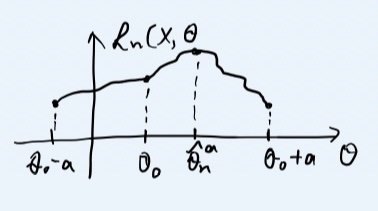
\includegraphics[scale=0.6]{lec2image1}
		\end{center}
		\item $\forall n$ при $w \in S_n$ может существовать целое множество корней $\{\theta_n^{*}\}$. Выберем в этом множестве корень $\hat{\theta_n}$, ближайший к $\theta_0$ (инфимум в множестве корней). Это можно сделать, т.к. функция $\frac{\partial}{\partial \theta} Ln (x, \theta)$ непрерывна по $\theta$, и последовательность корней есть тоже корень. Этот корень $\hat{\theta_n}$ и есть состоятельная оценка $\theta$, покажем это.\\
		$\text{Т.к. } S_n^{\varepsilon} \subseteq S_n, \; (w: |\hat{\theta_n}^{\varepsilon} - \theta_0| < \varepsilon) \subseteq (w: |\hat{\theta_n} - \theta_0| < \varepsilon)$, то для любого малого $\varepsilon > 0$:
		$$P_{\theta_0} (|\hat{\theta_n} - \theta_0| < \varepsilon, S_n) \ge P_{\theta_0}(|\hat{\theta_n}^{\varepsilon} - \theta_0| < \varepsilon, S_n^{\varepsilon})\eqno(3)$$
		$$\begin{gathered}
			\text{Но } P_{\theta_0}(|\hat{\theta_n}^{\varepsilon} - \theta_0| < \varepsilon, S_n^{\varepsilon}) = P_{\theta_0} (S_n^{\varepsilon}) \to 1 \; \Rightarrow \\
			\Rightarrow \text{ в силу } (3) \;  P_{\theta_0} (|\hat{\theta_n} - \theta_0| < \varepsilon, S_n) \to 1 \; \Rightarrow \; \text{пункт } (2) \text{ доказан}. 
		\end{gathered}$$
	\end{enumerate}
\end{Proof}

\begin{remark}\label{lec:2/remark:1}
	Определим следующую величину:
	$$\theta_n^{*} = \begin{cases}
		\text{сост. корень } \hat{\theta_n} \text{ ур-ния правдоподобия, если он} \exists \\
		\theta', \; \theta' \in \Theta, \text{ в противном случае}.
	\end{cases}\eqno(4)$$

	Тогда случайная величина $\theta_n^{*}$ всегда определена и $\theta_n^{*} \xrightarrow[]{P}\theta_0$, т.к. 
	$$P(|\theta_n^{*} - \theta_0| < \varepsilon) = P(|\hat{\theta_n} - \theta_0| < \varepsilon, S_n) + P(|\theta' - \theta| < \varepsilon, \overline{S_n}) \to 1.$$
	Ясно, что $\frac{\partial}{\partial \theta} Ln (x, \theta_n^{*}) = o (1)$, т.к. производная отлична от нуля только на $\overline{S_n}$.
\end{remark}

\begin{definition}\label{lec:2/def:6}
	Будем называть $\theta_n^{*}$ \red{обощенным корнем уравнения правдоподобия} $(2)$.
\end{definition}

\begin{theorem}[\blue{об асимптотической эффективности состоятельного решения}]\label{lec:2/the:3}
	Пусть $X = (X_1, \dots, X_n), \; \{X_i\}$ - н.о.р.с.в. Удовлетворяются условия теоремы Бахадура, в которых условия $(iii)$ и $(vi)$ заменены на предположение о третьей, а не второй производной, т.е. $|\frac{\partial^3}{\partial \theta^3} \ln f(x, \theta)| < M(x) \; \forall x \in N_f, \theta \in \Theta$ и $E_{\theta_0} M(x_1) < \infty$. Тогда, если $\theta_n^{*}$ - обощенный состоятельный корень уравнения правдоподобия из $(4)$, то $\sqrt{n}(\theta_n^{*} - \theta_0) \xrightarrow[]{d}N(0, \frac{1}{i(\theta)})$, т.е. $\theta_n^{*}$ - асимптотически эффективная оценка.
\end{theorem}
\begin{Proof}
	Будем обозначать $\frac{\partial}{\partial \theta}Ln (x, \theta), \frac{\partial^2}{\partial \theta^2}Ln (x, \theta), \dots$ через $Ln' (\theta), Ln^{(2)} (\theta), \dots$.

	Для фиксированного $X$ в силу формулы Тейлора и замечания из предыдущей лекции:
	$$\begin{gathered}
		\overline{o_p}(1) = Ln' (\theta_n^{*}) = Ln' (\theta_0) + Ln^{(2)}(\theta_0) (\theta_n^{*} - \theta_0) + \frac{1}{2} Ln^{(3)} (\tilde{\theta_n}) (\theta_n^{*} - \theta_0)^2, \; \tilde{\theta_n} \in (\theta_0, \theta_n^{*})
	\end{gathered}$$
	После преобразований получаем выражение:
	$$\sqrt{n}(\theta_n^{*} - \theta_0) = -\frac{n^{-\frac{1}{2}}Ln'(\theta_0) + \overline{o_p}(1)}{n^{-1}Ln^{(2)}(\theta_0)+ \frac{1}{2n} Ln^{(3)}(\tilde{\theta_n}) (\theta_n^{*} - \theta_0)}\eqno(5)$$
	Рассмотрим числитель $(5)$:
	$$n^{-\frac{1}{2}}Ln'(\theta_0) = n^{-\frac{1}{2}}\underset{i=1}{\overset{n}{\sum}}\frac{f'_{\theta}(x_i, \theta_0)}{f(x_i, \theta_0)} \xrightarrow[]{d}\xi \sim N(0, i(\theta_0))\eqno(6)$$
	Действительно:
	$$\begin{gathered}
		E_{\theta_0} \frac{f'_{\theta}(x_1, \theta_0)}{f(x_1, \theta_0)} = \underset{N_f}{\overset{}{\int}}\frac{f'_{\theta}(x, \theta_0)}{f(x, \theta_0)}f(x, \theta_0) \nu(dx) = 0\\
		\text{где } N_f \text{носитель плотности вероятности } f, \; f \ge 0\\
		D_{\theta_0}\frac{f'_{\theta}(x_1, \theta_0)}{f(x_1, \theta_0)} = E_{\theta_0} (\frac{\partial}{\partial \theta} \ln f(x_1, \theta_0))^2 = i(\theta_0)
	\end{gathered}$$
	Получаем, что величины $\{\frac{f'_{\theta}(x_i, \theta_0)}{f(x_i, \theta_0)}, i = \ton n\}$ - н.о.р. и соотношение $(6)$ следует из ЦПТ. Т.о. в силу леммы Слуцкого числитель $(5)$ сходится по вероятности к $N(0, i(\theta_0))$.\\

	Рассмотрим знаменатель $(5)$:
	$$n^{-1} Ln^{(2)} (\theta_0) = n^{-1} \underset{i=1}{\overset{n}{\sum}}\left[ \frac{f_{\theta}^{(2)}(x_i, \theta_0)}{f(x_i, \theta_0)}-(\frac{f'_{\theta}(x_i, \theta_0)}{f(x_i, \theta_0)})^2 \right] \xrightarrow[]{P} -i(\theta_0) \eqno(7)$$
	$$\frac{f_{\theta}^{(2)}(x_i, \theta_0)}{f(x_i, \theta_0)}-(\frac{f'_{\theta}(x_i, \theta_0)}{f(x_i, \theta_0)})^2 \text{ - производная от 1-ой производной по правилу Лейбница}$$
	Действительно, в силу ЗБЧ - хотелось бы применить слабый ЗБЧ в форме Чебышева, но там нужна дисперсия, поэтому воспользуемся ЗБЧ в форме Колмогорова, из которого получим сходимость почти наверно:
	$$\begin{gathered}
		\frac{1}{n}\underset{i=1}{\overset{n}{\sum}}\frac{f_{\theta}^{(2) (x, \theta_0)}}{f(x_i, \theta_0)} \xrightarrow[\text{если } \exists \text{ МО}]{P} E_{\theta_0} \frac{f_{\theta}^{(2)} (x_1, \theta_0)}{f(x_1, \theta_0)} = \underset{N_f}{\overset{}{\int}}\frac{f_{\theta}^{(2)} (x, \theta_0)}{f(x, \theta_0)} f(x, \theta_0) \nu(dx) = 0 \\
		\left(\frac{f_{\theta}^{(2) (x, \theta_0)}}{f(x_i, \theta_0)} \text{ - борелевские функции, н.о.р.с.в.}\right)\\
		\frac{1}{n}\underset{i=1}{\overset{n}{\sum}}(\frac{f'_{\theta} (x_i, \theta_0)}{f(x_i, \theta_0)})^2 \xrightarrow[]{P} E_{\theta_0} (\frac{\partial}{\partial \theta}\ln f(x_1, \theta_0))^2 = i(\theta_0)
	\end{gathered}$$
	Применяя лемму Слуцкого, получаем $(7)$ (сходимость к $-i(\theta_0)$).\\

	Рассмотрим второе слагаемое в знаменателе $(5)$:
	$$\begin{gathered}
		\left| \frac{1}{2n} Ln^{(3)} (\tilde{\theta_n}) (\theta_n^{*} - \theta_0) \right| \le \frac{1}{n} |\theta_n^{*} - \theta_0|\cdot \frac{1}{n}\underset{i=1}{\overset{n}{\sum}}M(x_i)\\
		\left(Ln^{(3)} (\tilde{\theta_n}) \le \underset{i=1}{\overset{n}{\sum}}M(x_i) \text{ (из условия)}\right)\\
		|\theta_n^{*} - \theta_0| \xrightarrow[]{P} 0, \; \frac{1}{n}\underset{i=1}{\overset{n}{\sum}}M(x_i) \xrightarrow[]{P} M \text{ - число} \text{ (в силу ЗБЧ)}
	\end{gathered}$$
	Тогда в силу леммы Слуцкого:
	$$\left| \frac{1}{2n} Ln^{(3)} (\tilde{\theta_n}) (\theta_n^{*} - \theta_0) \right| \xrightarrow[]{P}0\eqno(8)$$
	В силу $(7)$ и $(8)$ и леммы Слуцкого знаменатель в $(5)$ сходится по вероятности к $-i(\theta_0)$.\\
	Значит, по лемме Слуцкого вся дробь $(5)$ сходится по распределению к 
	$\frac{1}{i(\theta_0)} \xi \sim N(0, \frac{i(\theta_0)}{i^2 (\theta_0)}) = N(0, \frac{1}{i(\theta_0)})$, где $\xi$ - гауссовская случайная величина.
\end{Proof}

\section{ОМП для векторного параметра}\label{lec:3/sec:2}

Пусть $X = (X_1, \dots, X_n)$ - н.о.р., $X_1 \sim f(x, \theta)$, $\theta \in \Theta \subseteq \mathbb{R}^k$, $\Theta$ - открытое множество.\\

Логарифмическое правдоподобие имеет вид:
$$Ln (x, \theta) = \underset{i=1}{\overset{n}{\sum}}\ln f(x_i, \theta)$$
Система уравнений правдоподобия имеет вид:
$$\frac{\partial Ln (x, \theta)}{\partial \theta_i}=0, \; i=\ton k\eqno(9)$$
При условиях регулярности, похожих на условия теоремы \ref{lec:3/sec:1}, показывается:
\begin{enumerate}
	\item с вероятностью, стремящейся к $1$ при $n \to \infty$, система уравнений $(9)$ имеет такое решение $\hat{\theta_n} \in \Theta$, что $\hat{\theta_n}$ сходится к истинному значению $\theta_0$
	\item соответствующая оценка $\theta_n^{*}$ асимптотически нормальна, а именно:
	$$\begin{gathered}
		\sqrt{n} (\theta_n^{*} - \theta_0) \xrightarrow[n \to \infty]{d}N(o, I^{-1}(\theta_0))\\
		I(\theta) > 0 \text{ - \blue{матрица информации Фишера, }} I(\theta) = (I_{ij} (\theta)) \\
		I_{ij}(\theta) = E_{\theta} \left( \frac{\partial \ln f(x, \theta)}{\partial \theta_i} \cdot \frac{\partial \ln f(x, \theta)}{\partial \theta_j} \right)
	\end{gathered}$$
\end{enumerate}

\section{АЭО для интервала}\label{lec:3/sec:3}

\begin{example}\label{lec:3/example:1}
	Пусть $X = (X_1, \dots, X_n)$, где $\{X_i\}$ - н.о.р., $X_1 \sim N(\theta, \sigma^2), \; a < \theta < b$, т.е. $\Theta = (a,b)$. $a$ и $b$ - известные конечные числа, $\theta$ неизвестно, $\sigma^2$ известно. Необходимо построить АЭО.
\end{example}
\begin{solution}
	Построим АЭО $\theta_n^{*}$ для $\theta$.
	$$\begin{gathered}
		p(x, \theta) = (\frac{1}{\sqrt{2 \pi} \sigma})^n e^{-\frac{1}{2\sigma^2}\underset{i=1}{\overset{n}{\sum}}(x_i - \theta)^2} \text{ - плотность вероятности гауссовской сл. в.}\\
		Ln (x, \theta) = \ln (\frac{1}{\sqrt{2 \pi} \sigma})^n - \frac{1}{2 \sigma^2} \underset{i=1}{\overset{n}{\sum}}(x_i - \theta)^2\\
		- \frac{1}{2 \sigma^2} \underset{i=1}{\overset{n}{\sum}}(x_i - \theta)^2 \text{ - парабола ветвями вниз}
	\end{gathered}$$
	Уравнение правдоподобия имеет вид:
	$$\frac{\partial Ln (x, \theta)}{\partial \theta} = \frac{1}{\sigma^2}\underset{i=1}{\overset{n}{\sum}}(x_i - \theta) = 0$$
	Решение существует и единственно - это $\overline{X}$, причем в точке $\theta = \overline{X}$ функция $Ln (x, \theta)$ достигает максимума, т.к.:
	$$\frac{\partial^2 Ln(x, \overline{X})}{\partial \theta^2} = -\frac{1}{\sigma^2} < 0$$
	Т.о., если $a < \overline{X} < b$, то ОМП существует с вероятностью, стремящейся к $1$ и равна $\overline{X}$, в противном случае ОМП не существует.\\

	Если положить:
	$$\theta_n^{*} = \begin{cases}
		\overline{X}, \; a < \overline{X} < b \\
		\frac{a+b}{2} \text{ (любое число), } \overline{X} \not \in (a, b) 
	\end{cases}\eqno(9)$$
	то в силу теоремы \ref{lec:3/sec:1} (условия выполнены) $\theta_n^{*}$ - АЭО, т.е.:
	$$\sqrt{n}(\theta_n^{*} - \theta_0) \xrightarrow[]{d} N(0, \sigma^2), \; i(\theta) = \frac{1}{\sigma^2}\eqno(10)$$
	(также $(10)$ можно проверить непосредственно)
\end{solution}

\begin{remark}\label{lec:3/remark:1}
	Если $\theta \in [a,b]$, то по тоереме Вейерштрасса непрерывная функция на компакте достигает максимума и минимума. Тогда:
	$$\theta_n^{*} = \begin{cases}
		\overline{X}, \; \overline{X} \in (a, b)\\
		a, \; \overline{X} < a \\
		b, \; \overline{X} > b
	\end{cases}$$
	В $\theta = a$ или $\theta = b$ нет асимптотической гауссовости, поэтому надо рассматривать только открытые множества.
\end{remark}




\chapter{Проверка статистических гипотез}

Пусть $X = (X_1, \dots, X_n)$ (н.о.р.) имеет плотность вер-ти по мере $\mu$, $\theta \in \Theta \subseteq \mathbb{R}^k$.

\begin{definition}\label{lec:4/def:1}
	Предположение вида $H_0: \theta \in \Theta_0$, где $\Theta_0 \subseteq \Theta$, называется \red{параметрической гипотезой}.
\end{definition}

\begin{definition}\label{lec:4/def:2}
	\red{Альтернатива} $H_1: \theta \in \Theta_1, \Theta_1 = \Theta \setminus \Theta_0$. 
\end{definition}

\begin{definition}\label{lec:4/def:3}
	Если $\Theta_0 (\Theta_1)$ состоит из одной точки, то гипотеза $H_0$ (альтернатива $H_1$) называется \blue{простой}. В противном случае $H_0 (H_1)$ - \blue{сложная}.
\end{definition}

\green{Постановка задачи}\\
Необходимо построить правило (\blue{статистический критерий}), который позволяет заключить, согласуется ли $X$ с $H_0$ или нет.

\red{Правило}\\
Выберем в множестве значений $x$ вектора $X$ (либо $x = \mathbb{R}^n$, либо $x = N_p \subseteq \mathbb{R}^n$) подмножество $S$.
\begin{itemize}
	\item[-] если $X \in S$, то $H_0$ отвергается и принимается $H_1$
	\item[-] если $X \in \overline{S} = X \setminus S$, то $H_0$ принимается
\end{itemize}

\begin{definition}\label{lec:4/def:4}
	Множество $S$ называется \red{критическим множеством} или \red{критерием}, $\overline{S}$ - \blue{область принятия гипотезы}. 
\end{definition}

\green{Возможные ошибки}

\begin{definition}\label{lec:4/def:5}
	\red{Ошибка 1-го рода} - принять $H_1$, когда верна $H_0$. Вероятность ошибки 1-го рода: $\alpha = P(H_1 | H_0)$.
\end{definition}

\begin{definition}\label{lec:4/def:6}
	\red{Ошибка 2-го рода} - принять $H_0$, когда верна $H_1$. Вероятность ошибки 2-го рода: $\beta = P(H_0 | H_1)$.
\end{definition}

\begin{definition}\label{lec:4/def:7}
	\red{Мощностью критерия} $S$ называется функция $W (S, \theta) = W (\theta) := P_{\theta} (X \in S)$, т.е. мощность есть вероятность отвергнуть $H_0$, когда параметр равен $\theta$.
\end{definition}

$$\begin{gathered}
	\alpha = \alpha (\theta) = W(\theta), \theta \in \Theta_0 \\
	\beta = \beta (\theta) = 1 - W(\theta), \theta \in \Theta_1
\end{gathered}$$

\begin{remark}\label{lec:4/remark:1}
	Обычно $H_0$ более важна $\Rightarrow$ рассматривают критерии такие, что:
	$$\alpha (\theta) = W (\theta) = P_{\theta} (X \in S) \le \alpha \; \forall \theta \in \Theta_0$$
\end{remark}

\begin{definition}\label{lec:4/def:8}
	Число $\alpha$ называют \red{уровнем значимости} критерия и пишут $S_{\alpha}$.
\end{definition}

\begin{definition}\label{lec:4/def:9}
	Если критерий $S_{\alpha}^{*} \in \{S_{\alpha}\}$ и $\forall \theta \in \Theta_1$ и $\forall S_{\alpha}$ $W(S_{\alpha}*, \theta) \ge W(S_{\alpha}, \theta)$, то критерий $S_{\alpha}^{*}$ называется \red{РНМ-критерием} (равномерно наиболее мощным).
\end{definition}

Если $H_0: \theta = \theta_0, \; H_1: \theta = \theta_1$, т.е. $H_0$ и $H_1$ - простые, то задача отыскания РНМ-критерия заданного уровня $\alpha$ имеет вид:
$$\begin{gathered}
	P_{\theta_0} (X \in S_{\alpha}^{*}) \le \alpha \\
	P_{\theta_1} (X \in S_{\alpha}^{*}) \ge P_{\theta_1} (X \in S_{\alpha}) \; \forall S_{\alpha}
\end{gathered}$$

\section{Лемма Неймана-Пирсона}\label{lec:4/sec:2}

Положим для краткости:
$$p_0 (x) := p(x, \theta_0), p_1(x) = p(x, \theta_1), \; E_0 = E_{\theta_0}, \; E_1 = E_{\theta_1}$$

Введем множество: $S(\lambda) = \Set{x}{p_1(x) - \lambda p_0(x) > 0}, \; \lambda > 0$.

\begin{theorem}[\red{лемма Неймана-Пирсона}]\label{lec:4/the:1}
	Пусть для некоторого $\lambda > 0$ и критерия $R$ выполнено:
	\begin{itemize}
		\item[$(a)$] $P_0 (X \in R) \le P_0 (X \in S(\lambda))$
	\end{itemize}
	Тогда:
	\begin{itemize}
		\item[$(b)$] $P_1 (X \in R) \le P_1 (X \in S(\lambda))$
		\item[$(c)$] $P_1 (X \in S(\lambda)) \ge P_0 (X \in S(\lambda))$
	\end{itemize}
\end{theorem}

\begin{remark}\label{lec:4/remark:2}
	$x \in S(\lambda) \; \Leftrightarrow \; \frac{p_1 (x)}{p_0 (x)} > \lambda$
\end{remark}

\begin{definition}\label{lec:4/def:10}
	Т.к. $p_1(x)$ и $p_0(x)$ - правдоподобие, то критерий $S(\lambda)$ называется \red{критерием отношения правдоподобия Неймана-Пирсона}.
\end{definition}

\begin{remark}\label{lec:4/remark:3}
	Утверждение $(c)$ для $S(\lambda)$ означает, что
	$$P(H_1|H_1) \ge P(H_1|H_0) \; \Leftrightarrow \; W(S(\lambda), \theta_1) \ge W(S(\lambda), \theta_0)$$
	Это свойства называется \blue{несмещенностью} критерия $S(\lambda)$.
\end{remark}

\begin{Proof}
	Для краткости обозначим $S(\lambda) = S$.

	Пусть $I_R (x) = \begin{cases}
		1, x \in R \\
		0, x \not \in R
	\end{cases}$ Тогда: 
	$$(a) \; \Leftrightarrow \; E_0 I_R (x) \le E_0 I_S (x)\eqno(1)$$
	
	Докажем $(b)$. Верно неравенство:
	$$I_R (x) [p_1(x) - \lambda p_0(x)] \le I_S (x) [p_1(x) - \lambda p_0(x)]\eqno(2)$$
	Действительно:
	\begin{itemize}
		\item[-] если $p_1(x) - \lambda p_0(x) > 0$, то $I_S (x) = 1$ и $(2)$ очевидно
		\item[-] если $p_1(x) - \lambda p_0 (x) \le 0$, то правая часть $(2)$ есть ноль, а левая меньше либо равна нуля
	\end{itemize}
	Итак, $(2)$ верно. Интегрируем $(2)$ по $x \in \mathbb{R}^n$, получаем:
	$$E_1 I_R (x) - \lambda E_0 I_R (x) \le E_1 I_S (x) - \lambda E_0 I_S (x)$$
	$$E_1 I_S (x) - E_1 I_R (x) \ge \lambda [E_0 I_S (x) - E_0 I_R (x)]\eqno(3)$$
	$$(E_0 I_S (x) - E_0 I_R (x) \ge 0)$$
	В силу $(3)$ и $(1)$ и условия $\lambda >0$ получаем $E_1 I_S (x) \ge E_1 I_R (x)$, т.е. $(b)$ доказано.\\

	Докажем $(c)$. 
	\begin{itemize}
		\item[$1)$] Пусть $\lambda \ge 1$. Из определения $S$: $p_1(x) > p_0(x) \; \forall x \in S \; \Rightarrow$ 
		$$\begin{gathered}
			\Rightarrow \; P_0(X \in S) = \underset{\mathbb{R}^n}{\overset{}{\int}}I_S (x) p_0 (x) \mu (dx) \le \underset{\mathbb{R}^n}{\overset{}{\int}}I_S (x) p_1 (x) \mu (dx) = P_1 (X \in S) \\
			\text{т.е. } P(H_1|H_0) \le P(H_1|H_1)
		\end{gathered}$$
		\item[$2)$] Пусть $\lambda < 1$, $p_1 (x) < p_0 (x) \;\forall x \in \overline{S} \; \Rightarrow$
		$$\begin{gathered}
			\Rightarrow \; P_1(X \in \overline{S}) = \underset{\mathbb{R}^n}{\overset{}{\int}}I_{\overline{S}} (x) p_1 (x) \mu (dx) \le \underset{\mathbb{R}^n}{\overset{}{\int}}I_{\overline{S}} (x) p_0 (x) \mu (dx) = P_0 (X \in \overline{S}) \\
			\text{т.е. } 1 - P_1 (X \in S) \le 1 - P_0 (x \in S) \; \Rightarrow \; P_1(X \in S) \ge P_0(X \in S)
		\end{gathered}$$
	\end{itemize}
\end{Proof}

\section{Пример построения НМ-критерия}\label{lec:4/sec:3}

\begin{example}\label{lec:4/example:1}
	$X = (X_1, \dots, X_n)$, $\{X_i\}$ - н.о.р., $X_1 \sim N(\theta, \sigma^2)$, дисперсия $\sigma^2$ известна. Построим НМ-критерий для проверки:
	$\begin{cases}
		H_0: \theta = \theta_0 \\
		H_1: \theta = \theta_1, \theta_1 > \theta_0
	\end{cases}$

	Уровень значимости возьмем $\alpha$.
\end{example}
\begin{Proof}
	\begin{itemize}
		\item[$1)$] Имеем:
		$$\begin{gathered}
			p_0(x) = \left( \frac{1}{\sqrt{2 \pi} \sigma} \right)^n e^{-\frac{1}{2 \sigma^2} \underset{i=1}{\overset{n}{\sum}}(X_i - \theta_0)^2} \\
			p_1(x) = \left( \frac{1}{\sqrt{2 \pi} \sigma} \right)^n e^{-\frac{1}{2 \sigma^2} \underset{i=1}{\overset{n}{\sum}}(X_i - \theta_1)^2}
		\end{gathered}$$
		$$\begin{gathered}
			S(\lambda) = \Set{x}{p_1(x) - \lambda p_0(x) > 0} \; \Leftrightarrow \\
			\Leftrightarrow \; exp \{ -\frac{1}{2 \sigma^2} \underset{i=1}{\overset{n}{\sum}}[(X_i - \theta_1)^2-(X_i - \theta_0)^2] \} > \lambda \; \Leftrightarrow \\
			\Leftrightarrow \; \underset{i=1}{\overset{n}{\sum}}[(X_i - \theta_1)^2-(X_i - \theta_0)^2] < \lambda_1, \; \lambda_1 = -2 \sigma^2 \ln{\lambda} \; \Leftrightarrow \\
			\Leftrightarrow \; (\theta_0 - \theta_1) \underset{i=1}{\overset{n}{\sum}}X_i < \lambda_2 \; \Leftrightarrow \\
			\Leftrightarrow \;  \underset{i=1}{\overset{n}{\sum}}X_i > \tilde{\lambda}, \; \tilde{\lambda} = \tilde{\lambda} (\lambda, n, \sigma^2, \theta_0, \theta_1)
		\end{gathered}$$
		Итак: 
		$$S(\lambda) = \Set{x}{\underset{i=1}{\overset{n}{\sum}}X_i > \tilde{\lambda}} \text{ при некотором } \tilde{\lambda}$$
		\item[$2)$] Определим $\tilde{\lambda} = \tilde{\lambda_{\alpha}}$ из уравнения:
		$$\alpha = P_{\theta_0} (X \in S(\tilde{\lambda_{\alpha}})) = P_{\theta_0}(\underset{i=1}{\overset{n}{\sum}}X_i > \tilde{\lambda_{\alpha}})$$
		Тогда:
		$$\begin{gathered}
			\alpha = P_{\theta_0} (\frac{1}{\sqrt{n}\sigma} \underset{i=1}{\overset{n}{\sum}}(X_i - \theta_0) > \frac{\tilde{\lambda_{\alpha}} - n \theta_0}{\sqrt{n}\sigma}) = 1 - \Phi (\frac{\tilde{\lambda_{\alpha} - n \theta_0}}{\sqrt{n}\sigma}) \\
			\text{т.к.  } \frac{\underset{i=1}{\overset{n}{\sum}}(X_i - \theta_0)}{\sqrt{n}\sigma} \underset{H_0}{\sim} N(0,1) \text{. Значит, } \Phi (\frac{\tilde{\lambda_{\alpha} - n \theta_0}}{\sqrt{n}\sigma}) = 1-\alpha, \; \frac{\tilde{\lambda_{\alpha} - n \theta_0}}{\sqrt{n}\sigma} = \xi_{1-\alpha}\\
			\xi_{1-\alpha} \text{ - квантиль норм. закона уровня } \alpha\\
			\Phi (\dots) \text{ - функция Лампласа}
		\end{gathered}$$
		Итак:
		$$\tilde{\lambda_{\alpha}} = n \theta_0 + \sqrt{n} \sigma \xi_{1-\alpha}$$
		\item[$3)$] Положим:
		$$S_{\alpha}^{*} = \Set{x}{\underset{i=1}{\overset{n}{\sum}}X_i > \tilde{\lambda_{\alpha}}} \; \Rightarrow \; \begin{cases}
			P_{\theta_0} (X \in S_{\alpha}^{*}) = \alpha \\
			\forall S_{\alpha} \; P_{\theta_0} (X \in S_{\alpha}) \le \alpha = P_{\theta_0} (X \in S_{\alpha}^{*})
		\end{cases}$$ 
		Значит выполнено условие $(a)$ леммы Неймана-Пирсона, тогда в силу пункта $(b)$ этой леммы:
		$$P_{\theta_1} (X \in S_{\alpha}) \le P_{\theta_1} (X \in S_{\alpha}^{*})$$
		Таким образом, $S_{\alpha}^{*}$ - НМ-критерий.\\
		Т.к. $S_{\alpha}^{*}$ не зависит от $\theta_1$, то $S_{\alpha}^{*}$ - РНМ-критерий для $\begin{cases}
			H_0: \theta = \theta_1 \\
			H_1^{+}: \theta > \theta_1
		\end{cases}$

		Мощность критерия $S_{\alpha}^{*}$ для $H_0$ при альтернативе $H_1^{+}$:
		$$\begin{gathered}
			W(\theta, S_{\alpha}^{*}) = P_{\theta} (\underset{i=1}{\overset{n}{\sum}}X_i > n \theta_0 + \sqrt{n} \sigma \xi_{1-\alpha}) = \\
			= P_{\theta_0} \left( \frac{\underset{i=1}{\overset{n}{\sum}}(X_i - \theta_0)^2}{\sqrt{n} \sigma} > \frac{\sqrt{n} (\theta_0 - \theta)}{\sigma} + \xi_{1-\alpha} \right) = 1 - \Phi (\xi_{1-\alpha} + \frac{\sqrt{n} (\theta_0 - \theta)}{\sigma})
		\end{gathered}$$
		\begin{center}
			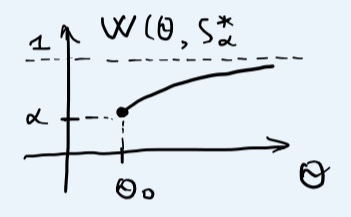
\includegraphics[scale=0.6]{lec4image1}
		\end{center}
	\end{itemize}
\end{Proof}

\section{Связь между доверительным оцениванием и проверкой гипотез}\label{lec:5/sec:1}

\begin{definition}\label{lec:5/def:1}
	Случайное подмножество $\Theta^* = \Theta^* (X, \alpha) \subseteq \Theta$ называется \red{доверительным интервалом} уровня $1-\alpha, 0 < \alpha < 1$, если
	$$P_{\theta} (\theta \in \Theta^* (X, \alpha)) \ge 1 - \alpha \; \forall \theta \in \Theta$$
\end{definition}

\begin{theorem}[]\label{lec:5/the:1}
	Докажем два пункта:
	\begin{enumerate}
		\item пусть $\forall \theta_0 \in \Theta$ гипотеза $H_0: \theta = \theta_0$ при альтернативе $H_1: \theta \not = \theta_0$ имеет $S_{\alpha}(\theta_0)$ критерий уровня $\alpha$. Пусть $\Theta^* (X, \alpha) = \Set{\theta}{x \in \overline{S_{\alpha}}(\theta_0)}$. Тогда $\Theta^* (X, \alpha)$ - доверительное множество уровня $1-\alpha$.
		\item Если $\Theta^* (X, \alpha)$ - доверительное множество уровня $1-\alpha$, то $\overline{S_{\alpha}}(\theta_0) = \Set{x}{\theta_0 \in \Theta^* (X, \alpha)}$ - область принятия гипотезы $H_0$.
	\end{enumerate}
\end{theorem}

\begin{remark}\label{lec:5/remark:1}
	Пункт 2) означает, что если $\theta_0$ попало в доверительное множество $\Theta^* (X, \alpha)$, то $H_0$ надо принимать.
\end{remark}

\begin{Proof}
	\begin{enumerate}
		\item 
			$\displaystyle P_{\theta} (\theta \in \Theta^* (X, \alpha)) = P_{\theta} (x \in \overline{S_{\alpha}}(\theta)) = 1 - P_{\theta} (x \in S_{\alpha}(\theta)) \ge 1 - \alpha \; \forall \theta \in \Theta$, т.к. $P_{\theta}(x \in S_{\alpha}(\theta)) \leq \alpha$.
		\item 
			$\displaystyle P_{\theta_0} (x \in S_{\alpha}(\theta_0)) = 1 - P_{\theta_0}(x \in \overline{S_{\alpha}}(\theta_0)) = 1 - P_{\theta_0} (\theta_0 \in \Theta^*(X, \alpha)) \le 1 - (1-\alpha) = \alpha$, т.к. $\displaystyle P_{\theta_0} (\theta_0 \in \Theta^*(X, \alpha)) \ge 1 - \alpha$, т.е. $\displaystyle S_{\alpha}(\theta_0) \text{ - критерий уровня } \alpha$.
	\end{enumerate}
\end{Proof}

\begin{example}[]\label{lec:5/example:1}
	Пусть $X = (X_1, \dots, X_n), \; \{X_i\}$ - н.о.р., $X_1 \sim N(\theta, \sigma^2), \; \theta \in \mathbb{R}^1$. Построим критерий для $H_0: \theta = \theta_0$ против $H_1: \theta \not = \theta_0$. Уровень значимости будет $\alpha, \; 0 < \alpha < 1$.
\end{example}
\begin{Proof}
	Построим доверительное множество для $\theta$ уровня $1 - \alpha$. Пусть $\overline{X} = n^{-1} \underset{i=1}{\overset{n}{\sum}}X_i$ - оптимальная оценка $\theta$, тогда:
	$$\begin{gathered}
		\frac{n^{\frac{1}{2}}(\overline{X}-\theta)}{\sigma} \sim N(0,1), \;\;
		P_{\theta} \left( \left| \frac{n^{\frac{1}{2}}(\overline{X}-\theta)}{\sigma} \right| < \xi_{1 - \frac{\alpha}{2}} \right) = 1 - \alpha, \; \Phi (\xi_{1 - \frac{\alpha}{2}}) = 1 - \frac{\alpha}{2} \\
		\text{т.е. } \Theta^* (X, \alpha) = \Set{\theta}{\left| \frac{n^{\frac{1}{2}}(\overline{X}-\theta)}{\sigma} \right| < \xi_{1 - \frac{\alpha}{2}}}
	\end{gathered}$$
	В силу замечания к теореме \ref{lec:5/the:1}:
	$$\begin{gathered}
		S_{\alpha}(\theta_0) = \Set{x}{\left| \frac{n^{\frac{1}{2}}(\overline{X}-\theta)}{\sigma} \right| \ge \xi_{1 - \frac{\alpha}{2}}} \\
		S_{\alpha}(\theta_0) \text{ - есть критическое множество для } H_0 \\
		\text{мощность } W(\theta) = P_{\theta} (x \in S_{\alpha}(\theta_0)) = P_{\theta} \left( \left| \frac{n^{\frac{1}{2}}(\overline{X}-\theta)}{\sigma} \right| \ge \xi_{1 - \frac{\alpha}{2}} \right) = \\
		= 1 - P_{\theta} \left( \left| \frac{n^{\frac{1}{2}}(\overline{X}-\theta)}{\sigma} \right| < \xi_{1 - \frac{\alpha}{2}} \right) = \\
		= 1 - P_{\theta}\left( -\xi_{1 - \frac{\alpha}{2}} + \frac{n^{\frac{1}{2}}(\theta_0-\theta)}{\sigma} \le \frac{n^{\frac{1}{2}}(\overline{X}-\theta)}{\sigma} \le \xi_{1 - \frac{\alpha}{2}} + \frac{n^{\frac{1}{2}}(\theta_0-\theta)}{\sigma} \right) = \\
		\bigg( \; \frac{n^{\frac{1}{2}}(\overline{X}-\theta)}{\sigma} \sim N(0,1) \; \bigg) \\ 
		= 1 - \left[ \Phi\left( \xi_{1 - \frac{\alpha}{2}} + \frac{n^{\frac{1}{2}}(\theta_0-\theta)}{\sigma} \right) - \Phi \left( -\xi_{1 - \frac{\alpha}{2}} + \frac{n^{\frac{1}{2}}(\theta_0-\theta)}{\sigma} \right) \right] = \\
		= \Phi\left( \xi_{1 - \frac{\alpha}{2}} + \frac{n^{\frac{1}{2}}(\theta_0-\theta)}{\sigma} \right) + \Phi\left( \xi_{1 - \frac{\alpha}{2}} + \frac{n^{\frac{1}{2}}(\theta-\theta_0)}{\sigma} \right)
	\end{gathered}$$
	\begin{multicols}{2}
			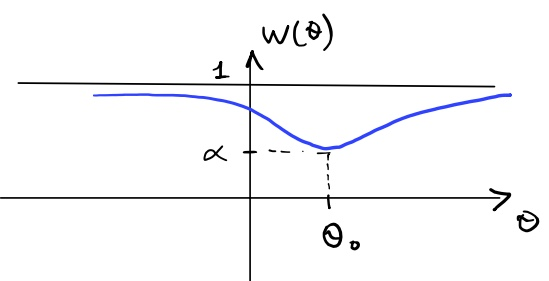
\includegraphics[scale=0.45]{lec5image1}

		\columnbreak

			\hfill \break
			$$\begin{gathered}
				W' (\theta_0) = 0 \\
				W(\theta) \xrightarrow[n \to \infty]{}1 \; \forall \theta \not = \theta_0
			\end{gathered}$$
	\end{multicols}
	Т.е. $S_{\alpha}(\theta_0)$ состоятелен против любой фиксированной инициативы.
\end{Proof}

\section{Критерий Фишера (F-критерий) в гауссовской линейной регрессии}\label{lec:5/sec:2}

\begin{definition}\label{lec:5/def:2}
	Если $\xi \sim N(0,1), \; \eta_k \sim \chi^2(k)$, $\xi$ и $\eta_k$ независимы, константа $\mu \in \mathbb{R}^1$, то
	$$\text{сл.в. } t_k (\mu) \Ddef \frac{\xi + \mu}{\sqrt{\frac{1}{k} \eta_k}} \sim S(k, \mu)$$
	имеет \red{нецентральное распределение Стьюдента} с $k$ степенями свободы и параметром нецентральности $\mu$.
\end{definition}

\begin{definition}\label{lec:5/def:3}
	Если $\xi_i \sim N(a_i, 1), i =\ton k$ и $\{\xi_1, \dots, \xi_k\}$ независимы, $\triangle^2 = a_1^2 + \dots + a_k^2$, то
	$$\text{сл.в. } \eta_k (\triangle) \Ddef \xi_1^2 + \dots + \xi_k^2 \sim \chi^2 (k, \triangle^2)$$
	имеет \red{нецентральное распределение хи-квадрат} с $k$ степенями свободы и параметром нецентральности $\triangle^2$.
\end{definition}

\begin{definition}\label{lec:5/def:4}
	Если $\eta_k \sim \chi^2 (k, \triangle^2), \; \nu_m \sim \chi^2 (m)$, и $\eta_k$ и $\nu_m$ независимы, то
	$$\text{сл.в. } f_{k,m} (\triangle) \Ddef \frac{\frac{1}{k}\eta_k}{\frac{1}{m}\nu_m} \sim F(k,m,\triangle^2)$$
	имеет \red{нецентральное распределение Фишера} с $(k,m)$ степенями свободы и параметром нецентральности $\triangle^2$.
\end{definition}

\begin{lemma}\label{lec:5/lemma:1}
	Докажем два пунтка:
	\begin{enumerate}
		\item распределение сл.в. $\eta_k \sim \chi^2 (k, \triangle^2)$ зависит лишь от $\triangle$, но не от $a_1, \dots, a_k$, а именно
		$$\eta_k \Ddef (z_1 + \triangle)^2 + z_2^2 + \dots + z_k^2$$
		где $\{z_1, \dots, z_k\}$ - н.о.р. $N(0,1)$ сл.в.
		\item если вектор $\xi \in \mathbb{R}^k, \; \xi \sim N(a, \Sigma), \; \Sigma > 0$, то 
		$$\xi^T \Sigma^{-1} \xi \sim \chi^2 (k, \triangle^2), \; \triangle^2 = a^T \Sigma^{-1} a$$
	\end{enumerate}
\end{lemma}
\begin{Proof}
	\begin{enumerate}
		\item По определению:
		$$\begin{gathered}
			\eta_k = \eta_k (\triangle) \Ddef \xi_1^2 + \dots + \xi_k^2 \\
			\{\xi_1, \dots, \xi_k\} \text{ - независимые } N(a_i, 1) \text{ сл.в.}
		\end{gathered}$$
		Пусть $\xi = (\xi_1, \dots, \xi_k)^T$.\\
		Ортогональная матрица $C = \begin{pmatrix}
			\frac{a_1}{\triangle} & \dots & \frac{a_k}{\triangle} \\
			\dots & \dots & \dots
		\end{pmatrix}, \; \nu = C \xi$.\\
		Тогда $\eta_k \Ddef |\xi|^2 = |\nu|^2$, т.к. $C$ - ортогональная, но
		$$\begin{gathered}
			\nu = C \begin{pmatrix}
			a_1 \\ \vdots \\ a_k
		\end{pmatrix} + C \overset{o}{\xi} = \begin{pmatrix}
			\triangle \\ 0 \\ \vdots \\ 0
		\end{pmatrix} + Z \\
		\text{где } \overset{o}{\xi} = \xi - E \xi, \; Z = C \overset{o}{\xi} \sim N(0, E_k), \text{ таким образом:}\\
		\eta_k \Ddef |\nu|^2 = (z_1 + \triangle)^2 + z_2^2 + \dots + z_k^2
		\end{gathered}$$
		\item 
		$\displaystyle \xi^T \Sigma^{-1} \xi = |\Sigma^{-\frac{1}{2}}\xi|^2, \text{ причем } \Sigma^{-\frac{1}{2}} \xi \sim N(\Sigma^{-\frac{1}{2}} a, E_k)$, тогда: 
		$$\displaystyle |\Sigma^{-\frac{1}{2}} \xi|^2 \sim \chi^2 (k, \triangle^2), \; \triangle^2 = |\Sigma^{-\frac{1}{2}}a|^2 = a^T \Sigma^{-1} a$$
	\end{enumerate}
\end{Proof}

\begin{lemma}\label{lec:5/lemma:2}
	Случайная величина $t_k (\mu)$ обладает следующим свойством стохастической упорядоченности:
	\begin{itemize}
		\item[(4)] при $\mu_2 > \mu_1$ и при $\forall x \in \mathbb{R}^1$ $P(t_k (\mu_2) > x) > P(t_k (\mu_1) > x)$
		\item[(5)] $P(\eta_k (\triangle_2) > x) > P(\eta_k (\triangle_1) > x), \; \triangle_2 > \triangle_1$
		\item[(6)] $P(f_{k,m} (\triangle_2) > x) > P(f_{k,m} (\triangle_1) > x), \; \triangle_2 > \triangle_1$
	\end{itemize}
\end{lemma}
\begin{Proof}
	Заметим, что если $\xi$ и $\eta$ - независимые сл. вел. и $E|\varphi(\xi, \eta)|< \infty, \; \varphi$ -- борелевская функция, то 
	$$E \varphi(\xi, \eta) = E \{\left( E \varphi(\xi, \eta) \right)|_{y = \eta}\}\eqno(7)$$
	В силу (7):
	$$\begin{gathered}
		P(t_k (\mu_2) > x) = P \left( \frac{\xi + \mu_2}{\sqrt{\frac{1}{k}\eta_k}} > x \right) = E \mathbb{I} \left(\xi > x \sqrt{\frac{1}{k}\eta_k} - \mu_2 \right) = \\
		= E \left\{ 1 - \mathbb{I}\left( \xi \le x \sqrt{\frac{1}{k} \eta_k} - \mu_2 \right) \right\} = 1 - E \left\{ \left( E \mathbb{I} (\xi \le y) \right)|_{y = x \sqrt{\frac{1}{k}\eta_k} - \mu_2} \right\} = \\
		= 1 - E \Phi \left( x \sqrt{\frac{1}{k}\eta_k} - \mu_2 \right) > 1 - E \Phi \left( x \sqrt{\frac{1}{k}\eta_k} - \mu_1 \right) = P \left( t_k (\mu_1) > x \right)
	\end{gathered}$$
	$$\left( \text{т.к. } E \Phi \left( x \sqrt{\frac{1}{k}\eta_k} - \mu_2 \right) < E \Phi \left( x \sqrt{\frac{1}{k}\eta_k} - \mu_1 \right) \text{ в силу возрастания } \Phi \right)$$
\end{Proof}

\section{Построение доверительного множества для линейной гауссовской модели}\label{lec:6/sec:1}

Пусть $X = Z c + \varepsilon$, где $X = (X_1, \dots, X_n)^T$ - наблюдение.\\
$Z$ - $(n\times p)$-матрица регрессора, $rk Z = p, \; p < n$.\\
$\varepsilon \sim N(0, \sigma^2 E_n), \; c = (c_1, \dots, c_p)^T$, $c$ и $\sigma^2$ неизвестны.\\

Рассмотрим новый вектор $\beta = A c$, $A$ - $(k \times p)$-матрица, $rk A = k \le p$, т.е. строки $A$ линейно независимы. Построим для $\beta$ доверительное множество уровня $1-\alpha$.
\begin{solution}
	Пусть $\hat{c_n}$ - о.н.к. для $c$ (также оптимальная).\\
	Пусть $\hat{S_n}^2$ - о.н.к. для $\sigma^2$. Пусть $\hat{\beta_n} = A \hat{c_n}$ - оптимальная оценка для $\beta$.\\
	Т.к. $\hat{c_n} \sim N(c, \sigma^2 (Z^T Z)^{-1})$, то $\hat{\beta_n} \sim N(Ac, \sigma^2 D)$, где $Ac = \beta, \; D = A (Z^T Z)^{-1} A^T$.\\

	Заметим, что $D > 0$, т.к. для $\alpha \in \mathbb{R}^k, \; \alpha \not = 0, \; \alpha^T D \alpha = (A^T \alpha)^T (Z^T Z)^{-1} (A^T \alpha) > 0$, поскольку $(Z^T Z)^{-1} > c, \; A^T \alpha \not = 0$ при $rk A = k$ и $\alpha \not = 0$.\\

	В силу пункта 2) леммы \ref{lec:5/lemma:1}: $\frac{1}{\sigma^2} (\hat{\beta_n} - \beta)^T D^{-1} (\hat{\beta_n} - \beta) \sim \chi^2 (k)$\\

	Т.к. $\frac{(n-p) \hat{S_n}^2}{\sigma^2} \sim \chi^2 (n-p), \; \hat{\beta_n}$ и $\hat{S_n}^2$ независимо, то
	$$\begin{gathered}
		f_{k, n-p} (X, \beta) := \frac{\frac{\frac{1}{k}(\hat{\beta_n}-\beta)D^{-1} (\hat{\beta_n} - \beta)}{\sigma^2}}{\frac{\frac{1}{n-p} (n-p) \hat{S_n}^2}{\sigma^2}} = \frac{(\hat{\beta_n}-\beta)D^{-1} (\hat{\beta_n} - \beta)}{k \hat{S_n}^2} \sim F(k, n-p) \; \Rightarrow \\
		P_{\beta, \sigma^2} \left( (\hat{\beta_n}-\beta)D^{-1} (\hat{\beta_n} - \beta) \le k \hat{S_n}^2 f_{1-\alpha}(k,n-p) \right) = 1 - \alpha \\
		f_{1-\alpha}(k,n-p) \text{ - квантиль уровня } 1-\alpha \text{ распределения } F(k,n-p) 
	\end{gathered}$$
	Доверительное множество для $\beta$ уровня $1-\alpha$:
	$$\begin{gathered}
		\Theta^* (X, \alpha) = \Set{\beta}{(\hat{\beta_n}-\beta)D^{-1} (\hat{\beta_n} - \beta) < k \hat{S_n}^2 f_{1-\alpha}(k,n-p)} \\
		(\text{\red{доверительный эллипсоид}})
	\end{gathered}$$
\end{solution}

\hfill \break
Рассмотрим теперь проверку гипотезы $H_0: \beta = \beta_0$ против $H_1: \beta \not = \beta_0$.

\begin{definition}\label{lec:6/def:1}
	$H_0$ называется \red{линейной гипотезой}, т.к. $\beta = A c$ получается линейным преобразованием $c$.
\end{definition}

В силу замечания \ref{lec:5/remark:1} $H_0$ надо принимать, если $\beta_0 \in \Theta^* (X, \alpha)$, т.е. область принятия $H_0$:
$$\overline{S_{\alpha}}(\beta_0) = \Set{x}{f_{k, n-p}(x, \beta_0) \le f_{1-\alpha}(k,n-p)}$$
т.е. критическое множество (критерий уровня $\alpha$):
$$S_{\alpha}(\beta_0) = \Set{x}{f_{k,n-p}(x, \beta_0) > f_{1-\alpha}(k,n-p)}\eqno(7)$$

\begin{definition}\label{lec:6/def:2}
	Критерий (7) называется \red{критерием Фишера} \\ \red{(F-критерием)}, а $f_{k,n-p}(x, \beta_0)$ - \red{статистикой F-критерия}.
\end{definition}

Рассмотрим поведение F-критерия при альтернативе $H_1$: при $H_1$ в силу пункта 2 леммы \ref{lec:5/lemma:1}:
$$\begin{gathered}
	f_{k, n-p}(x, \beta_0) = \frac{\frac{\frac{1}{k}(\hat{\beta_n}-\beta)D^{-1} (\hat{\beta_n} - \beta)}{\sigma^2}}{\frac{\frac{1}{n-p} (n-p) \hat{S_n}^2}{\sigma^2}}, \; \frac{(\hat{\beta_n}-\beta)D^{-1} (\hat{\beta_n} - \beta)}{\sigma^2} \sim \chi^2 (k, \triangle^2) \\
	\frac{(n-p) \hat{S_n}^2}{\sigma^2} \sim \chi^2 (n-p), \text{ тогда } f_{k, n-p}(x, \beta_0) \sim F(k,n-p, \triangle^2)
\end{gathered}$$
Параметр нецентральности: $\triangle^2 = \frac{1}{\sigma^2}(\beta - \beta_0)D^{-1}(\beta - \beta_0)$ \\

Мощность F-критерия:
$$\begin{gathered}
	W(\beta, S_{\alpha}(\beta_0)) = P_{\beta, \sigma^2} (f_{k,n-p}(x, \beta_0) > f_{1-\alpha}(k,n-p)) = 1 - F_{k,n-p}(f_{1-\alpha}(k,n-p), \triangle^2) \\
	\text{при } \beta = \beta_0 \;\; W(\beta_0, S_{\alpha}(\beta_0)) = \alpha
 \end{gathered}$$

\begin{properties}\label{lec:6/props:1}
	Свойства мощности:
	\begin{enumerate}
		\item $\triangle = \triangle (\beta) > 0 = \triangle (\beta_0)$ при $\beta \not = \beta_0$, тогда из соотношения (6) леммы \ref{lec:5/lemma:2}:
		$$P_{\beta, \sigma^2} (f_{k, n-p}(x, \beta_0) > f_{1-\alpha}(k,n-p)) > P_{\beta_0, \sigma^2} (f_{k,n-p}(x, \beta_0) > f_{1-\alpha} (k, n-p)) = \alpha$$
		т.е. при $\beta \not = \beta_0$ $P(H_1 | H_1) > P(H_1 | H_0)$,\\
		т.е. F-критерий \blue{несмещенный}
		\item мощность $W (\beta, S_{\alpha}(\beta_0))$ строго монотонна по $\triangle$ из соотношения (8)
	\end{enumerate}
\end{properties}

\section{Пример определения порядка регрессии}\label{lec:6/sec:2}
Пусть $c^T = (c_{(1)}^T, c_{(2)}^T)$, $c_{(1)}$ - $m$-вектор, $c_{(2)}$ - $p-m$-вектор, $1 \le m \le p$.

$H_0: c_{(2)} = 0$ (т.е. порядок $\le m$), $H_1: c_{(2)} \not = 0$.

Пусть матрица $A = \bordermatrix{
& {}_{\underline{1}} & \underline{\dots} & {}_{\underline{m}} & {}_{\underline{m+1}} & \underline{\dots} & {}_{\underline{p}} \cr
& 0 & \dots & 0 & 1 & \dots & 0 \cr
& \vdots & \ddots & \vdots & \vdots & \ddots & \vdots \cr
& 0 & \dots & 0 & 0 & \dots & 1 \cr}$, тогда $A c = c_{(2)}$ и \\ $H_0$ эквивалентна гипотезе $A c = 0 = \beta_0$ -- $p-m$-вектор.\\

Пусть $\hat{c_n}^T = (\hat{c_{(1)}}_n^T, \hat{c_{(2)}}_n^T)$, где $\hat{c_{(1)}}_n^T$ -- $m$-вектор, $\hat{c_{(2)}}_n^T$ -- $p-m$-вектор. Тогда $\hat{\beta_n} = A \hat{c_n} = \hat{c_{(2)}}_n$.
$$\begin{gathered}
	\text{Если } (Z^T Z)^{-1} = \bordermatrix{
& {}_{\underline{1\times m}} & {}_{\underline{(m+1)\times p}} \cr
\;\;{}_{1\times m}| & B_{11} & B_{12} \cr
{}_{(m+1)\times p}| & B_{21} & B_{22} \cr}, \\
 \text{то } D = A (Z^T Z)^{-1} A^T = B_{22}.
\end{gathered}$$
Тогда:
$$f_{p-m,n-p}(x, \beta_0=0) = \frac{\hat{c_{(2)}}_n^T B_{22}^{-1} \hat{c_{(2)}}_n}{(p-m)\hat{S_n}^2}$$
\begin{itemize}
	\item[$\bullet$] при $H_0$ $f_{p-m,n-p}(x,0) \sim F(p-m, n-p)$
	\item[$\bullet$] $H_0$ отвергается, если $f_{p-m,n-p}(x,0) > f_{1-\alpha}(p-m,n-p)$, т.е.
	$$ S_{\alpha}(0) = \Set{x}{\frac{\hat{c_{(2)}}_n^T B_{22}^{-1} \hat{c_{(2)}}_n}{(p-m)\hat{S_n}^2} > f_{1-\alpha}(p-m,n-p)} \eqno(9)$$
	\item[$\bullet$] при $H_1$ $f_{p-m, n-p}(x, 0) \sim F(p-m, n-p, \triangle^2)$, где
	$$ \triangle^2 = \frac{\hat{c_{(2)}}^T B_{22}^{-1} \hat{c_{(2)}}}{\sigma^2} \eqno(10)$$
	\item[$\bullet$] критерий (9) несмещенный, т.е. $P(H_1|H_1) > P(H_1|H_0) = \alpha$. Его мощность:
	$$\begin{gathered}
		W (c_{(2)}, S_{\alpha}(0)) = P_{c_{(2)}, \sigma^2} (f_{p-m,n-p}(x,0) > f_{1-\alpha}(p-m,n-p)) = \\
		= 1 - F_{p-m,n-p}(f_{1-\alpha}(p-m,n-p), \triangle^2) \\
		\text{т.е. мощность строго возрастает по } \triangle^2
	\end{gathered}$$
	Параметр нецентральности $\triangle^2$ определен в (10)
\end{itemize}

\section{Пример проверки однородности двух выборок}\label{lec:6/sec:3}

Пусть $X = (X_1, \dots, X_m), \; Y = (Y_1, \dots, Y_m)$ - две независимые гауссовские выборки, т.е. 
$\{X_i\}$ - н.о.р., $X_1 \sim N(a, \sigma^2)$, $\{Y_j\}$ - н.о.р., $Y_1 \sim N(b, \sigma^2)$.
Совокупности $\{X_i\}$ и $\{Y_j\}$ независимы, $m+n > 2$. Дисперсии $D X_1 = D Y_1 = \sigma^2$ и неизвестны, средние $a$ и $b$ неизвестны.\\

Проверим гипотезу $H_0: a = b$ против $H_1: a \not = b$ по наблюдениям $X$ и $Y$. Гипотеза $H_0$ называется \red{гипотезой однородности}.

При $D X_1 \not = D X_2$ описанная задача называется \blue{проблемой Беренса-Фишера}.\\

Итак:
$$\begin{cases}
	X_i = a + \varepsilon_i, \; i =\ton m, \; \; \varepsilon_i := X_i - a \\
	Y_j = b + \tilde{\varepsilon_j}, \; j =\ton n, \;\; \tilde{\varepsilon_j} := Y_j - b
\end{cases}$$
Тогда $\varepsilon_1, \dots, \varepsilon_m, \tilde{\varepsilon_1}, \dots, \tilde{\varepsilon_n}$ - н.о.р. $N(0, \sigma^2)$ с.в.\\
Пусть $\tilde{X} = (X_1, \dots, X_m, Y_1, \dots, Y_n)^T, \; c = (a,b)^T, \; \varepsilon^T = ( \varepsilon_1, \dots, \varepsilon_m, \tilde{\varepsilon_1}, \dots, \tilde{\varepsilon_n} )^T$

$$Z = \bordermatrix{
& \cr
\;1| & 1 & 0 \cr
\;\; \vdots| & \vdots & \vdots \cr 
\;m| & 1 & 0 \cr
{}_{m+1}| & 0 & 1 \cr
\;\; \vdots| & \vdots & \vdots \cr
{}_{m+n}| & 0 & 1 \cr
} \; \Rightarrow \; \tilde{X} = Z c + \varepsilon\eqno(11)$$

Соотношение (11) определяет гауссовскую линейную регрессию.\\

Положим $A = (1,-1)\; \Rightarrow \; A c = a - b = \beta$.
$$\begin{gathered}
	H_0: A c = a - b = \beta = 0 \; (= \beta_0) \\
	H_1: A c = a - b  \not = 0 \; (\text{т.е. } \beta \not = 0)
\end{gathered}$$

Тогда, о.н.к. для вектора $c$ - это решение задачи.
$$\underset{i=1}{\overset{m}{\sum}}(X_i - a)^2 + \underset{j=1}{\overset{n}{\sum}}(Y_j - b)^2 \to \underset{a,b}{min}\eqno(12)$$
Задача (12) эквивалентна системе уравнений:
$$\begin{cases}
	-2 \underset{i=1}{\overset{m}{\sum}}(X_i - a) = 0 \\
	-2 \underset{j=1}{\overset{n}{\sum}}(Y_j - b) = 0
\end{cases}$$
Решения этой системы $\hat{a_n} = \overline{X}, \; \hat{b_n} = \overline{Y}$ - оптимальные оценки $a$ и $b$. $\hat{c_n} = (\overline{X}, \overline{Y})^T$ - оптимальная оценка $c$. Оптимальная оценка для $\sigma^2$:
$$\hat{S_{m+n}}^2 = \frac{1}{m+n-2}\left[ \underset{i=1}{\overset{m}{\sum}}(X_i - \overline{X})^2 + \underset{j=1}{\overset{n}{\sum}}(Y_j - \overline{Y})^2 \right]$$
Тогда $\hat{\beta_n} = A \hat{c_n} = \overline{X} - \overline{Y}$.
$$\begin{gathered}
	Z^T Z = \bordermatrix{
	& \underline{{}_{1}} & \underline{\dots} & \underline{{}_{m}} & \underline{{}_{m+1}} & \underline{\dots} & \underline{{}_{m+n}} \cr
	& 1 & \dots & 1 & 0 & \dots & 0 \cr
	& 0 & \dots & 0 & 1 & \dots & 1
} \begin{pmatrix}
	1 & 0 \\
	\vdots & \vdots \\
	1 & 0 \\
	0 & 1 \\
	\vdots & \vdots \\
	0 & 1
\end{pmatrix} = \begin{pmatrix}
	m & 0 \\
	0 & n
\end{pmatrix} \\
D = A (Z^T Z)^{-1} A^T = \begin{pmatrix}
	1 & -1
\end{pmatrix} \begin{pmatrix}
	\frac{1}{m} & 0 \\
	0 & \frac{1}{n}
\end{pmatrix} \begin{pmatrix}
	1 \\ -1
\end{pmatrix} = \frac{1}{n} + \frac{1}{m}
\end{gathered}$$ 
Значит:
$$f_{1,m+n-2} (X, \beta_0 = 0) = \frac{(\overline{X} - \overline{Y})^2}{\left( \frac{1}{n} + \frac{1}{m} \right) \hat{S_{m+n}}^2}$$
F-критерий для $H_0$ имеет вид:
$$S_{\alpha} (0) = \Set{x \in\mathbb{R}^{m+n}}{f_{1, m+n-2}(X, 0) > f_{1-\alpha}(1,m+n-2)}$$
При $H_0$ (т.е. при $a=b$) $f_{1,m+n-2} (X,0) \sim F(1,m+n-2)$.\\
При $H_1$ (т.е. при $a\not=b$) $f_{1,m+n-2} (X,0) \sim F(1,m+n-2, \triangle^2)$.\\
Параметр нецентральности:
$$\triangle^2 = \triangle^2 (\beta) = \triangle^2 (a-b) = \frac{(a-b)^2}{\sigma^2 \left( \frac{1}{m} + \frac{1}{n} \right)}$$
\begin{enumerate}
	\item если $|a-b|$ возрастает, то мощность F-теста тоже возрастает
	\item если $\sigma \to 0$ или $\frac{1}{m} + \frac{1}{n} \to 0$, то мощность возрастает
\end{enumerate}

\section{Проверка простой гипотезы в схеме Бернулли}\label{lec:7/sec:1}

Пусть проводится $n$ независимых испытаний и в каждом испытании возможны $m$ исходов, $m \ge 2$, $A_1, \dots, A_m$ таких, что $A_i A_j = \emptyset$ при $i \not = j, \; \underset{}{\overset{}{\sum}}A_i = \Omega$. $P(A_j) = p_j > 0, \; \underset{j=1}{\overset{m}{\sum}}p_j = 1$. Пусть $\nu = (\nu_1, \dots, \nu_m)^T$, а $\nu_j$ - число появлений $A_j$ в $n$ опытах $X \; \Rightarrow \; \underset{j=1}{\overset{m}{\sum}}\nu_j = n$.\\
По вектору наблюдений $\nu$ необходимо проверить гипотезу $H_0$:

$H_0: p_j = p_j^0, \; j = 1, \dots, m$. 

Альтернатива $H_1: p_j \not = p_j^0$ хотя бы при одном $j$. 

Подчеркнем, что $H_0$ - простая гипотеза, т.к. она полностью определяет распределение вектора $\nu$, а именно при $H_0$:
$$\begin{gathered}
	P(\nu_1 = k_1, \dots, \nu_m = k_m) = \frac{n!}{k_1! \dots k_m!} (p_1^0)^{k_1} \dots (p_m^0)^{k_m} \text{ -- } \\
	\text{это полиномиальное распределение } \Pi (n, p_1^0, \dots, p_m^0)
\end{gathered}$$ 

Статистика хи-квадрат Пирсона для $H_0$ имеет вид:
$$\chi_n^2 := \underset{j=1}{\overset{m}{\sum}}\frac{(\nu_j - n p_j^0)^2}{n p_j^0}$$
Поведение при альтернативе: очевидно, что
$$\chi_n^2 = n \underset{j=1}{\overset{m}{\sum}}\frac{(\frac{\nu_j}{n} - p_j^0)^2}{p_j^0}$$
В силу теоремы Бернулли:
$$\begin{gathered}
	\frac{\nu_j}{n} \xrightarrow[]{P} p_j \; \Rightarrow \; \underset{j=1}{\overset{m}{\sum}}\frac{(\frac{\nu_j}{n} - p_j^0)^2}{p_j^0} \xrightarrow[]{P} \underset{j=1}{\overset{m}{\sum}}\frac{(p_j - p_j^0)^2}{p_j^0} > 0 \text{ при } H_1 \\
	\text{(по теореме о наследовании сходимости по вероятности)}
\end{gathered}$$
Значит, при $H_1$ $\chi_n^2 \xrightarrow[n \to \infty]{P}\infty$, поэтому большие значения $\chi_n^2$ свидетельстуют против $H_0$. Но что такое большие значения?

\begin{theorem}[\red{Пирсона}]\label{lec:7/the:1}
	При $H_0$ и $n \to \infty$ $\chi_n^2 \xrightarrow[]{d} \chi^2 (m-1)$.
\end{theorem}

\begin{rulee}\label{lec:7/rule:1}
	Если $\chi_n^2 > \chi_{1-\alpha}(m-1)$, то $H_0$ отвергаем и принимаем $H_1$. Если $\chi_n^2 \le \chi_{1-\alpha}(m-1)$, то принимаем $H_0$.

	Тогда:
	$$\begin{gathered}
		P(H_1 | H_0) = P(\chi_n^2 > \chi_{1-\alpha} (m-1)) \to \alpha \\
		P(H_0 | H_1) = P(\chi_n^2 \le \chi_{1-\alpha} (m-1) | H_1) \xrightarrow[n\to \infty]{}0 \\
		\text{т.е. } \begin{cases}
			P(H_0 | H_0) \to 1 - \alpha \\
			P(H_1 | H_1) \to 1
		\end{cases}
	\end{gathered}$$
	Вероятность принять правильную гипотезу близка к единице.
\end{rulee}


\section{Проверка простой гипотезы о виде функции распределения}\label{lec:7/sec:2}

Пусть $X = (X_1, \dots, X_n)$, $\{X_i\}$ - н.о.р., $X_1 \sim F(x)$.\\
$H_0: F(x) = F_0 (x)$, $F_0$ полностью известна.\\
$H_1: F(x) = F_1 (x)$ и $F_1 (x) \not = F_0 (x)$.\\

Разобьем носитель $X_1$ на непересекающиеся отрезки $\triangle_1, \dots, \triangle_m$ так, что \\
$(m \ge 2)$ $X_1 \in \triangle_1 \bigcup \dots \bigcup \triangle_m$.
$$p_j^0 := P(x_1 \in \triangle_j | H_0) = \underset{\triangle_j}{\overset{}{\int}}d F_0 (x) > 0 \; \forall j \; \Rightarrow \; \underset{j=1}{\overset{m}{\sum}}p_j^0 = 1$$
С каждой величиной $X_i$ свяжем испытание с исходами $A_1, \dots, A_m$, причем $A_j$ происходит тогда и только тогда, когда $X_i \in \triangle_j$.\\
При $H_0$ $P(A_j) = p_j^0$, тогда наблюдения $X_1, \dots, X_n$ порождают полиномиальную схему независимых испытаний. \\
Пусть $\nu_j$ - число исхода $A_j$ в этих испытаниях, т.е. число наблюдений среди $X_1, \dots, X_n$, попавших в $\triangle_j$.\\
В силу теоремы Пирсона при $H_0$:
$$\chi_n^2 := \underset{j=1}{\overset{m}{\sum}}\frac{(\nu_j - n p_j^0)^2}{n p_j^0} \xrightarrow[]{d}\chi^2 (m-1)$$

\begin{rulee}\label{lec:7/rule:2}
	$H_0$ будем отвергать, если $\chi_n^2 > \chi_{1-\alpha} (m-1) \; \Rightarrow \; P(H_1 | H_0) \xrightarrow[n\to \infty]{}\alpha$.

	Если верна $H_1$ и хотя бы при одном $j$ $p_j := P(X_1 \in \triangle_j | H_1) = \underset{\triangle_j}{\overset{}{\int}}d F_1 (x) \not = p_j^0$, то $P(H_0 | H_1) = P(\chi_n^2 < \chi_{1-\alpha}(m-1)|H_0) \to 0$
\end{rulee}

\begin{remark}\label{lec:7/remark:1}
	Если $F_0 \not \equiv F_1$, но $p_j = p_j^0 \; \forall j$, то $P(H_0 | H_1) = P(H_0 | H_0) \to 1- \alpha \not = 0$. Например:
	\begin{multicols}{2}
			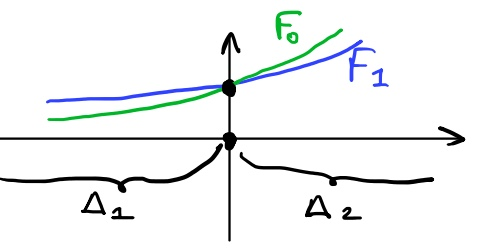
\includegraphics[scale=0.5]{lec7image1}

		\columnbreak
			$$\begin{gathered}
				m=2 \\
				P(X_1 \in \triangle_1 | H_0) = F_0 (0) = \\
				= P(X_1 \in \triangle_1 | H_1) = F_1(0) \\
				P(X_1 \in \triangle_2 | H_0) = 1 - F_0 (0) = \\
				=  P(X_1 \in \triangle_2 | H_1) = 1 - F_1(0)
			\end{gathered}$$
	\end{multicols}
\end{remark}

\begin{Proof}
	(доказательство теоремы Пирсона)\\

	Покажем, что вектор $\nu = (\nu_1, \dots, \nu_m)^T$ асимптотически нормален, т.е.
	$$ n^{\frac{1}{2}} (n^{-1}\nu - p) \xrightarrow[]{d} N(0, P - p p^T) \eqno(13)$$
	где $P = \begin{pmatrix}
		p_1^0 & \dots & 0 \\
		\vdots & \ddots & \vdots \\
		0 & \dots & p_m^0
	\end{pmatrix}$, $p = (p_1^0, \dots, p_m^0)^T$.

	Для этого введем вектора $X_1, \dots, X_n$, где $X_i = (0, \dots, 0, 1, 0, \dots, 0)^T$ с 1 на j-ом месте, если в $i$-ом испытании произошло $A_j$, тогда: $\nu = \sum\limits_{i = 1}^n X_i,$
	$$ n^{\frac{1}{2}} (n^{-1} \nu - p) = n^{\frac{1}{2}} \underset{i=1}{\overset{n}{\sum}}(X_i - p) \eqno(14)$$
	В (14) $\{X_i\}$ - н.о.р., $E X_1 = p$.
	$$cov (X_1, X_1) = E(X_1 - p)(X_1 - p)^T = E X_1 X_1^T - p p^T = P - p p^T$$
	Поэтому соотношение (13) следует из представления (14) и ЦПТ.\\
	Матрица $P - p p^T$ вырождена, т.к. сумма $r$ столбцов есть ноль:

	если $e = (1, \dots, 1)^T$, то $(P - p p^T) e = p - p (p^T e) = p - p = 0$.\\

	Пусть $P^{-\frac{1}{2}} = \begin{pmatrix}
		\frac{1}{\sqrt{p_1^0}} & \dots & 0 \\
		\vdots & \ddots & \vdots \\
		0 & \dots & \frac{1}{\sqrt{p_m^0}}
	\end{pmatrix}, \;\; \xi_n := n^{\frac{1}{2}} P^{-\frac{1}{2}} (n^{-1} \nu - p)$.

	В силу теоремы о наследовании слабой сходимости и соотношения (13):
	$$\begin{gathered}
		(H(x) = P^{-\frac{1}{2}} x, \; x \in \mathbb{R}^m) \\
		\xi_n \xrightarrow[]{d} N(0, P^{-\frac{1}{2}} (P - p p^T)(P^{-\frac{1}{2}})^T)
	\end{gathered}$$
	Но $P^{-\frac{1}{2}} (P - p p^T)(P^{-\frac{1}{2}})^T = E_m - Z Z^T$, где $Z = (\sqrt{p_1^0}, \dots, \sqrt{p_m^0})^T$. Тогда:
	$$ \xi_n \xrightarrow[]{d} N(0, E_m - Z Z^T) \eqno(15)$$
	Пусть ортогональная матрица $U = \begin{pmatrix}
		\sqrt{p_1^0} & \dots & \sqrt{p_m^0} \\
		\dots & \dots & \dots
	\end{pmatrix}$. Тогда:
	$$\begin{gathered}
		U (E_m - Z Z^T)U^T = E_m - (U Z)(U Z)^T = \begin{pmatrix}
		1 & \dots & 0 \\
		\vdots & \ddots & \vdots \\
		0 & \dots & 1
	\end{pmatrix} - \begin{pmatrix}
		1 \\ 0 \\ \vdots \\ 0
	\end{pmatrix} \begin{pmatrix}
		1 & 0 & \dots & 0
	\end{pmatrix} = \\
	= \begin{pmatrix}
		0 & 0 & \dots & 0 \\
		0 & 1 & \dots & 0 \\
		\vdots & \vdots & \ddots & \vdots \\
		0 & 0 & \dots & 1
	\end{pmatrix} = \tilde{E_1}
	\end{gathered}$$
	В силу (15) и теоремы о наследовании слабой сходимости:
	$$ U \xi_n \xrightarrow[]{d} N(0, \tilde{E_1}) \eqno(16)$$
	т.е. $U \xi_n \xrightarrow[]{d} (0, \eta_2, \dots, \eta_m)^T, \; \{\eta_2, \dots, \eta_m\}$ - нез. $N(0,1)$ с.в.\\

	Из (16) опять в силу теоремы о наследовании слабой сходимости:
	$$ |U \xi_n|^2 \xrightarrow[]{d} \eta_2^2 + \dots + \eta_m^2 \sim \chi^2 (m-1) \eqno(17)$$
	Осталось заметить, что:
	$$|U \xi_n|^2 = |\xi_n|^2 = \underset{j=1}{\overset{m}{\sum}}\left[ \frac{1}{\sqrt{p_j^0}} n^{\frac{1}{2}} (n^{-1} \nu_j - p_j^0) \right]^2 = \underset{j=1}{\overset{m}{\sum}}\frac{(\nu_j - n p_j^0)^2}{n p_j^0} = \chi_n^2$$
	Последнее равенство и соотношение (17) доказывают теорему Пирсона.
\end{Proof}

\section{Проверка сложной гипотезы в схеме испытаний Бернулли}\label{lec:8/sec:1}

Пусть проводится $n$ независимых испытаний, исходы $A_1, \dots, A_m$, $\nu = (\nu_1, \dots, \nu_m)^T$ - вектор наблюдений.\\
Пусть $H_0: p(A_j) = p_j (\theta), \; \theta \in \Theta \subseteq \mathbb{R}^k, \; k < m-1$.\\

\vspace{2cm}
\textbf{\blue{Условия регулярности:}}
\begin{itemize}
	\item[(i)] $\underset{j=1}{\overset{m}{\sum}}p_j (\theta) = 1 \; \forall \theta \in \Theta$
	\item[(ii)] $p_j (\theta) \ge c > 0$ для $j =\ton m$ и $\exists \frac{\partial p_j (\theta)}{\partial \theta_l}, \; \frac{\partial^2 p_j (\theta)}{\partial \theta_l \partial \theta_r}$
	\item[(iii)] $rk \left( \frac{\partial p_j (\theta)}{\partial \theta_l} \right) = k \; \forall \theta \in \Theta, \frac{\partial p_j (\theta)}{\partial \theta_l}$ - $m\times k$-матрица
\end{itemize}

В качестве оценки $\theta$ при $H_0$ будем использовать мультиноминальные оценки максимального правдоподобия:
$$P(\nu_1 = k_1, \dots, \nu_m = k_m) = \frac{n!}{k_1! \dots k_m!} p_1^{k_1} (\theta) \dots p_m^{k_m} (\theta)$$
Логарифм правдоподобия:
$$Ln (\nu, \theta) = \ln \frac{n!}{\nu_1! \dots \nu_m!} + \underset{j=1}{\overset{m}{\sum}}\nu_j \ln p_j (\theta)$$
О.м.п. (мультиномиальная): $Ln (\nu, \theta) \to \underset{\theta \in \Theta}{max}$.

\begin{theorem}[\red{Фишера}]\label{lec:8/the:1}
	Пусть верна $H_0$, пусть выполнены условия $(i)-(iii)$, пусть $\theta_n$ - мультиномиальная о.м.п., $\hat{\chi_n}^2 := \underset{j=1}{\overset{m}{\sum}}\frac{(\nu_j - n p_j (\hat{\theta_n}))^2}{n p_j (\hat{\theta})}$. \\
	Тогда $\hat{\chi_n}^2 \xrightarrow[]{d} \chi(m-k-1)$.
\end{theorem}

\begin{rulee}\label{lec:8/rule:1}
	Если $\hat{\chi_n}^2 > \chi_{1-\alpha}(m-k-1)$, то $H_0$ отвергаем, тогда $P(\overline{H_0}|H_0)\to \alpha$.
\end{rulee}

\section{Проверка независимости признаков}\label{lec:8/sec:2}

Пусть объект классифицирован по двум признакам $A$ и $B$, $A = \{A_1, \dots, A_s\}$, $B = \{B_1, \dots, B_r\}$, причем $s,r > 1$.\\
Проводится $n$ опытов, пусть $\nu_{ij}$ - число объектов, имеющих признаки $A_i B_j$, пусть $p_{ij} = P(A_i B_j)$.\\

Гипотеза независимости $H_0: p_{ij} = p_{i\cdot} p_{\cdot j}$ для положительных $p_{i \cdot}$ и $p_{\cdot j}$ таких, что $\underset{i=1}{\overset{s}{\sum}}p_{i \cdot} = 1$, $\underset{j=1}{\overset{r}{\sum}}p_{\cdot j} = 1$.\\
При $H_0$ логарифимческое правдоподобие:
$$Ln (\nu, p_{i \cdot}, p_{\cdot j}) = \ln \frac{n!}{\underset{ij}{\Pi} \nu_{ij}} + \underset{i=1}{\overset{s}{\sum}}\underset{j=1}{\overset{r}{\sum}}\nu_{ij} (\ln p_{i \cdot} + \ln p_{\cdot j})$$
Максимизируя эту функцию по $p_{i \cdot}, p_{\cdot j}$ при условиях $\underset{i=1}{\overset{s}{\sum}}p_{i \cdot} = 1$ и $\underset{j=1}{\overset{r}{\sum}}p_{\cdot j} = 1$, находим оценки:
$$\hat{p_{i \cdot}} = \frac{\nu_{i \cdot}}{n}, \; \hat{p_{\cdot j}} = \frac{\nu_{\cdot j}}{n}, \text{ где } \nu_{i \cdot} = \underset{j=1}{\overset{r}{\sum}}\nu_{ij}, \; \nu_{\cdot j} = \underset{i=1}{\overset{s}{\sum}}\nu_{ij}$$
Статистика хи-квадрат имеет вид:
$$\hat{\chi_n}^2 = \underset{i=1}{\overset{s}{\sum}}\underset{j=1}{\overset{r}{\sum}}\frac{(\nu_{ij} - n \hat{p_{i \cdot}}\hat{p_{\cdot j}})^2}{n \hat{p_{i \cdot}}\hat{p_{\cdot j}}}$$
При $H_0$ $\hat{\chi_n}^2 \xrightarrow[]{d} \chi \left( (s-1)(r-1) \right)$, т.к. число разбиений $m-k-1 = s r - (s+r-2)-1 = (s-1)(r-1)$.

\begin{rulee}\label{lec:8/rule:2}
	Если $\hat{\chi_n}^2 > \chi_{1-\alpha} \left( (s-1)(r-1) \right)$, то $H_0$ отвергается, асимптотический уровень теста равен $\alpha$.
\end{rulee}

\textbf{\green{Числовой пример}} (W.H. Gilby, Biometrika)\\
1725 школьников классифицировали (1) в соответствии с качеством их одежды и (2) в соответствии с их умственными способностями. Использовали следующую градацию:

\begin{center}
	\begin{tabular}{| c | c |}
		\hline
		градация & характеристика \\ \hline \hline
		A & умственно отсталый \\ \hline
		B & медлительный и тупой\\ \hline
		C & тупой\\ \hline
		D & медлительный, но умный\\ \hline
		E & достаточно умный\\ \hline
		F & явно способный\\ \hline
		G & очень способный\\ \hline
	\end{tabular}
\end{center}
$H_0:$ признаки независимы.

\begin{center}
  \begin{tabular}{ | l || c | c | c | c | c | c || r |}
    \hline
    как одевается? & \blue{A и B} & \blue{C} & \blue{D} & \blue{E} & \blue{F} & \blue{G} & \blue{Сумма} \\ \hline \hline
    \blue{очень хорошо} & 33 & 48 & 113 & 209 & 194 & 39 & 636  \\ \hline
    \blue{хорошо} & 41 & 100 & 202 & 255 & 138 & 15 & 751  \\ \hline
    \blue{сносно} & 39 & 58 & 70 & 61 & 33 & 4 & 265  \\ \hline
    \blue{очень плохо} & 17 & 13 & 22 & 10 & 10 & 1 & 73  \\ \hline \hline
    \blue{сумма} & 130 & 219 & 407 & 535 & 375 & 59 & 1725 \\ \hline
  \end{tabular}
\end{center}

Здесь $\chi_n^2 = 174.92 > \chi_{0.999} (15) = 37.697$, здесь $(s-1)(r-1) = (4-1)(6-1)=15$, т.е. $H_0$ отвергается.












\chapter{Введение в робастное оценивание}

Схема, предложенная Мартином-Йохаи (Martin, Yohai, 1986), имеет вид:
$$y_t = u_t + z_t^{\gamma} \xi_t, \; t = \ton n$$
\begin{itemize}
 	\item[$\bullet$] здесь $\{u_t\}$ - <<полезный сигнал>> (временной ряд)
 	\item[$\bullet$] $\{z_t^{\gamma}\}$ - н.о.р.с.в., $z_1^{\gamma} \sim Bin (1, \gamma)$ с $0 \le \gamma \le 1$, $\gamma$ - уровень засорения
 	\item[$\bullet$] $\xi_t$ - н.о.р.с.в. - грубые выбросы, $\xi_1$ имеет распределение $\mu_{\xi} \in M_{\xi}$, распределение $\mu_{\xi}$ неизвестно, а множество $M_{\xi}$ известно
 	\item[$\bullet$] последовательности $\{u_t\}, \{z_t^{\gamma}\}, \{\xi_t\}$ независимы между собой
 \end{itemize} 

 Пусть $y_1, \dots, y_n$ - наблюдения, и распределение вектора $Y_n = (y_1, \dots, y_n)$ зависит от неизвестного параметра $\beta$. Пусть $\hat{\beta_n}$ - некоторая оценка $\beta$.\\

 \textbf{Основное предположение}\\
При любом $0 \le \gamma \le 1$ существует предел $\hat{\beta_n} \xrightarrow[n \to \infty]{P}\theta_{\gamma}, \; \theta_0 = \beta$, т.е. $\hat{\beta_n}$ состоятельна.

\begin{definition}\label{lec:8/def:1}
	Если существует предел
	$$IF (\theta_{\gamma}, \mu_{\xi}) := \underset{\gamma \to +0}{\overset{}{\lim}} \frac{\theta_{\gamma} - \theta_0}{\gamma}$$
	то $IF(\theta_{\gamma}, \mu_{\xi})$ называется \red{функционалом влияния} (influence function) оценки $\hat{\beta_n}$.
\end{definition}

Если функционал влияния существует, то
$$\theta_{\gamma} = \theta_0 + IF (\theta_{\gamma}, \mu_{\xi}) \gamma + \overline{o}(\gamma), \; \gamma \to +0$$
т.е. $IF (\theta_{\gamma}, \mu_{\xi})$ характеризует главный линейный по $\gamma$ член в разложении по $\gamma$ асимптотического смещения $\theta_{\gamma} - \theta_0 = \theta_{\gamma} - \beta$.

\begin{definition}\label{lec:8/def:2}
	Величина $CES (\theta_{\gamma}, M_{\xi}) := \underset{\mu_{\xi} \in M_{\xi}}{\sup} |IF (\theta_{\gamma}, \mu_{\xi})|$ (cross error sensivity) называется \red{чувствительностью} оценки $\hat{\beta_n}$ к засорениям (выбросам).
\end{definition}

Если $CES (\theta_{\gamma}, M_{\xi}) < \infty$, то главный член по $\gamma$ асимптотического смещения $IF (\theta_{\gamma}, \mu_{\xi})\gamma$ равномерно мал при малых $\gamma$.

\begin{definition}\label{lec:8/def:3}
	Если $CES (\theta_{\gamma}, M_{\xi}) < \infty$, то оценка $\hat{\beta_n}$ называется \red{робастной} по смещению, или \red{B-робастной}.
\end{definition}

\section{Пример о выборочном среднем}\label{lec:8/sec:4}

$$\begin{cases}
	u_t = a + \varepsilon_t, \; \varepsilon_t \text{ - ошибки измерений} \\
	y_t = u_t + z_t^{\gamma} \xi_t, \; t = \ton n, \;\; E |\xi_1| < \infty
\end{cases}$$
$\{\varepsilon_t\}$ - н.о.р.с.в., $E \varepsilon_1 = 0 \; \Rightarrow \; E u_t = a$.

Возьмем оценкой $a$ эмпирическое среднее $\overline{y} = n^{-1}\underset{t=1}{\overset{n}{\sum}}y_t$ - о.н.к. ($\underset{t=1}{\overset{n}{\sum}}(y_t - \theta)^2 \to \underset{\theta}{min}$), тогда:
$$\begin{gathered}
	\overline{y} \xrightarrow[]{P}E(u_1 + z_1^{\gamma} \xi_1) \\
	\text{(по теореме Колмогорова)}\\
	E(u_1 + z_1^{\gamma} \xi_1) = a + \gamma E \xi_1 = \theta_{\gamma}^{LS}
\end{gathered}$$
Функция $\theta_{\gamma}^{LS}$ (least square) определена при всех $\gamma$.
$$\frac{\partial \theta_{\gamma}^{LS}}{\partial \gamma} = E \xi_1 = IF (\theta_{\gamma}, \mu_{\xi})$$
Если $M_1$ - класс распределений с конечным первым моментом, то
$$CES (\theta_{\gamma}^{LS}, M_1) = \underset{\mu_{\xi}\in M_1}{sup} |E{\xi_1}| = \infty$$
т.е. $\overline{y}$ - не B-робастна на классе $M_1$. 

\section{Пример о выборочной медиане}\label{lec:9/sec:1}
Пусть 
$$u_t = a + \varepsilon_t, \; t = \ton n \eqno(1)$$ где $\{\varepsilon_t\}$ - н.о.р.с.в., $\varepsilon_t \sim G(x)$ и ф.р. $G(x)$ неизвестна, $G(0) = \frac{1}{2}$. Тогда ф.р. $u_t$ есть $F(x) = G(x-a)$, т.е. $F(a) = \frac{1}{2}$. Итак, ноль - медиана $G(x)$, а $a$ - медиана $F(x)$.\\

Если $\varepsilon_t$ имеет симметричное относительно нуля распределение (т.е. $\varepsilon_t \Ddef -\varepsilon_t$, что для непрерывной $G(x)$ равносильно условию $G(x) + G(-x) = 1$ при всех $x$), то условия выше выполняются автоматически.

Т.о. при сформулированных условиях оценку медианы можно использовать как оценку математического ожидания.\\

Пусть $u_{(1)} \le u_{(2)} \le \dots \le u_{(n)}$ будет вариационный ряд наблюдений $u_1, \dots, u_n$.

\begin{definition}\label{lec:9/def:1}
	Величина $\hat{m_n} = \begin{cases}
		u_{(k+1)}, \; n = 2 k - 1 \\
		\frac{u_{(k+1)} + u_{(k)}}{2}, \; n = 2 k
	\end{cases}, k = 1, 2, \dots$ называется \red{выборочной медианой} наблюдений $u_1, \dots, u_n$.
\end{definition}

Мы знаем, что если $G(x)$ дифференцируема в нуле, и $g(0) = G' (0) > 0$, то для выборочной медианы справедлива асимптотическая нормальность:
$$n^{\frac{1}{2}} (\hat{m_n} - a) \xrightarrow[n \to \infty]{d} N \left(0, \frac{1}{4 g^2 (0)}\right)$$
Если в (1) $\{\varepsilon_t\}$ - н.о.р., $E \varepsilon_t = 0, \; 0 < E \varepsilon_t^2 = \sigma^2 < \infty$, то $n^{\frac{1}{2}} (\overline{u} - a) \xrightarrow[n \to \infty]{d} N(0, \sigma^2)$. Значит АОЭ выборочной медианы относительно $\overline{u}$ равна $e_{\hat{m_n}, \overline{X}} = 4 g^2 (0) \sigma^2$.\\

Изучим B-робастность выборочной медианы. Пусть:
$$\begin{gathered}
	\begin{cases}
		u_t = a + \varepsilon_t \\
		y_t = u_t + z_t^{\gamma} \xi_t, \; t = \ton n
	\end{cases} \\
	\hat{m}_n^y = \begin{cases}
		y_{(k+1)}, n = 2k-1 \\
		\frac{y_{(k)} + y_{(k+1)}}{2}, n = 2k
	\end{cases}
\end{gathered}$$

\begin{theorem}[]\label{lec:9/the:1}
	Пусть существует производная $g(x) = G' (x)$, $g(x)$ непрерывна и ограничена, $g(0) > 0$, $G(0) = \frac{1}{2}$. Тогда:
	\begin{itemize}
		\item[1)] $\hat{m}_n^y \xrightarrow[n \to \infty]{P}\theta_{\gamma}^m$, $\theta_0 = a$
		\item[2)] существует функционал влияния выборочной медианы
		$$IF (\theta_{\gamma}^m, \mu_{\xi}) = \frac{1 - 2 E G(-\xi_1)}{2 g(0)}$$
		\item[3)] чувствительность выборочной медианы на классе всех возможных распределений $M_{\xi}$
		$$GES (\theta_{\gamma}^m, M_{\xi}) = \underset{\mu_{\xi} \in M_{\xi}}{\sup}|IF (\theta_{\gamma}^m, \mu_{\xi})| = \frac{1}{2 g(0)} < \infty$$
		т.е. выборочная медиана B-робастна.
	\end{itemize}
\end{theorem}
\begin{Proof}

	\textit{ШАГ 1}.\\
	Выборочная медиана $\hat{m}_n^y$ удовлетворяет уравнению:
	$$l_n (\theta) := n^{-1} \underset{t=1}{\overset{n}{\sum}}sign (y_t - \theta) = 0\eqno(2)$$
	где $sign (x) = \begin{cases}
		-1, x < 0 \\
		0, x = 0 \\
		1, x > 1
	\end{cases}$

	Справедливость (2) легко понять из рисунков:
	\begin{figure}[h]
		\begin{multicols}{2}
			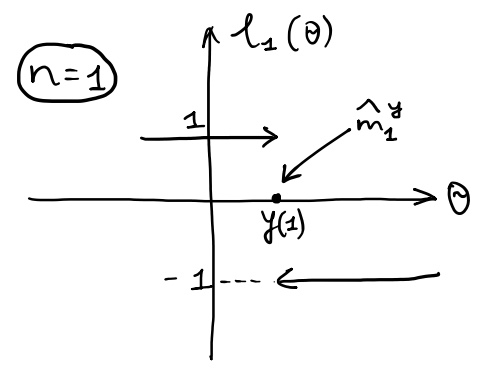
\includegraphics[width=90mm]{lec9im1}
			\columnbreak
			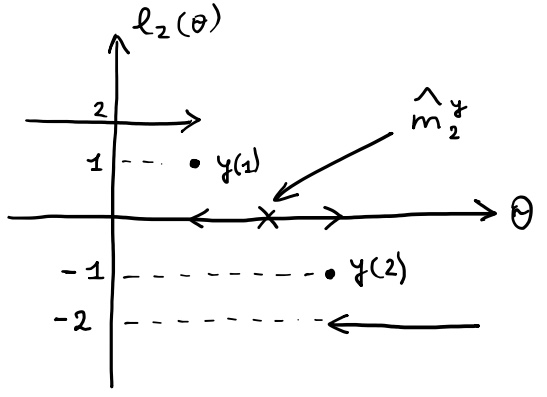
\includegraphics[width=90mm]{lec9im2}
		\end{multicols}
	\end{figure}

	Так бывает всегда: при нечетном $n$ решение уравнения (2) всегда существует и единственно - это $\hat{m}_n^y$; при четном $n$ решений целый интервал и $\hat{m}_n^y$ - его середина.

	В силу ЗБЧ при любом $\theta$ и любом $0 \le \gamma \le 1$:
	$$l_n (\theta) = n^{-1} \underset{t=1}{\overset{n}{\sum}}sign (y_t - \theta) \xrightarrow[n \to \infty]{P} E sign(y_1 - \theta) =: \Lambda_M (\gamma, \theta)$$

	\begin{problem} Пусть $\xi, \; \eta$ -- независимые случайные векторы, причем $\eta$ -- дискретный вектор со значениями $\eta_1, \eta_2, \ldots$. Необходимо проверить, что 
	$$E\varphi(\xi, \eta) = \sum\limits_{k \geq 1} E\varphi(\xi, \eta_k)P(\eta = \eta_k) = \sum\limits_{k \geq 1} E(\varphi(\xi, \eta) | H_k)P(H_k),$$ 
	где гипотеза $H_k = (\eta = \eta_k)$.
	\end{problem}

	Найдем удобный вид для $\Lambda_M(\gamma, \theta)$. Имеем
	$$\Lambda_M(\gamma, \theta) = E(1- 2 I(y_1 - \theta \leq 0)) = 1 - 2EI(\varepsilon_1 \leq \theta - a - z^{\gamma}_1 \xi_1) = 1 - 2EG(\theta - a - z^{\gamma}_1 \xi_1), \eqno(3)$$
	т.к. $sign(x) = 1 - 2I(x < 0)$ при $x \neq 0$.

	Чтобы упростить (3), введем две гипотезы: $H_1 = (z^{\gamma}_1 = 0), \; H_2 = (z^{\gamma}_2 = 1)$. Тогда, используя задачу, получим из (3), что $$\Lambda_M(\gamma, \theta) = 1 - 2(1 - \gamma)G(\theta - a) - 2\gamma EG(\theta - a - \xi_1).$$ Функция $\Lambda_M(\gamma, \theta)$ определена при всех $\gamma, \; \theta$, в том числе для отрицательных $\gamma$.

	\textit{ШАГ 2}.\\
	Функция $\Lambda_M(\gamma, \theta)$ в окрестности точки (0, a) удовлетворяет всем предположениям теоремы о неявной функции. А именно:

	\begin{enumerate}
		\item $\Lambda_M(0, a) = 1 - 2G(0) = 0;$
		\item Существуют и непрерывнф по паре $(\gamma, \theta)$ фнкции $\dfrac{\partial\Lambda_M(\gamma, \theta)}{\partial\gamma}, \; \dfrac{\partial\Lambda_M(\gamma, \theta)}{\partial\theta};$
		\item $\dfrac{\partial\Lambda_M(\gamma, \theta)}{\partial\theta} = -2g(0) \neq 0.$
	\end{enumerate}

	Значит, в окрестности точки (0, a) определена функция $\theta_m(\gamma) = \theta_{\gamma}^m$ такая, что $\Lambda_M(\gamma, \theta_{\gamma}^m) = 0.$ Кроме того, $\theta_{0}^m = a, \; \theta_{\gamma}^m \longrightarrow \theta_0$ при $\gamma \longrightarrow 0$. Функция $\theta_{\gamma}^m$ дифференцируема в точке $\gamma = 0$, и 
	$$\dfrac{d \theta_{\gamma}^m}{d\gamma} \mid_{\gamma = 0} = -(\dfrac{\partial \Lambda_M(0, a)}{\partial\theta})^{-1} \dfrac{\partial \Lambda_M(0, a)}{\partial\gamma} = \dfrac{1 - 2EG(-\xi_2)}{2g(0)} \eqno(4)$$

	\textit{ШАГ 3}.\\
	Покажем, что 
	$$\hat{m_n^y} \longrightarrow \theta_{\gamma}^m, \; n \longrightarrow \infty\eqno(5)$$
	Тогда из (4), (5) будет следовать, что функционал влияния  выборочной медианы равен 
	$$IF(\theta_{\gamma}^m, \mu_{\xi}) = \dfrac{1 - 2EG(-\xi_1)}{2g(0)}\eqno(6)$$
	Модуль числителя в (6) не больше 1, причем, если $\xi_1$ неслучайно и $\xi_1 \longrightarrow +\infty,$ то числитель стремится к 1. Значит, 
	$$GES(\theta_{\gamma}^m, M_{\xi}) = \underset{\mu_{\xi} \in M_{\xi}}{sup}|IF(\theta_{\gamma}^m, \mu_{\xi})| = \dfrac{1}{2g(0)}.$$
	Итак, докажем (5). Имеем при малых $\gamma$ ($\gamma$ фиксированно!) и $\theta$ вблизи a:
	$$\dfrac{\partial\Lambda_M(\gamma, \theta)}{\partial\theta} = -2(1 - \gamma)g(\theta - a) - 2\gamma Eg(\theta - a - \xi_1) < 0$$ 
	То есть $\Lambda(\gamma, \theta)$ убывает по $\theta.$ Значит,
	$$\begin{cases}
	\Lambda_M(\gamma, \theta_{\gamma}^m - \Delta) > 0 \\
	\Lambda_M(\gamma, \theta_{\gamma}^m + \Delta) < 0
	\end{cases},$$ но
	$$\begin{cases}
	l_n(\theta_{\gamma}^m - \Delta) \stackrel{P}{\longrightarrow} \Lambda_M(\gamma, \theta_{\gamma}^m - \Delta) > 0 \\
	l_n(\theta_{\gamma}^m + \Delta) \stackrel{P}{\longrightarrow} \Lambda_M(\gamma, \theta_{\gamma}^m + \Delta) < 0
	\end{cases} \eqno(7)$$
	Функция $l_n(\theta)$ монотонно убывает (точнее, не возрастет) по $\theta$. В силу (7) с вероятностью сколь угодно близкой к единице при достаточно больших n все корни уравнения $l_n(\theta) = 0$ лежат в интервале $(\theta_{\gamma}^m - \Delta, \theta_{\gamma}^m + \Delta)$. Выборочная медиана $\hat{m_n^y}$ тоже лежит в этом интервале! Поскольку $\Delta > 0$ любое, получаем, что 
	$$\hat{m_n^y} \stackrel{P}{\longrightarrow} \theta_{\gamma}^m, \; n \longrightarrow \infty.$$ 
\end{Proof}

\section{Нахождение функционала влияния в общем случае}\label{lec:9/sec:2}

Пусть оценка $\hat{\beta_n}$ ищется как корень уравнения
$$l_n(\theta) := n^{-1}\sum\limits_{t = 1}^n \varphi(\mathcal{I}_n, \theta) = 0 \eqno(1)$$
Пусть выполнены следующие условия:

 $$(i) l_n(\theta) = n^{-1}\sum\limits_{t = 1}^n \varphi(\mathcal{I}_n, \theta) \stackrel{P}{\longrightarrow} \Lambda(\gamma, \theta) \text{ при всех } |\theta - \beta| < \delta, \; 0 \geq \gamma < \gamma_0$$
 $$(ii) \Lambda(0, \beta) = 0$$
 $$\begin{gathered}(iii) \text{Пусть } \Lambda(\gamma, \theta) \text{ можно продолжить на отрицательные малые } \gamma \text{ так, что}\\ 
 \text{при }  |\theta - \beta| < \delta, \; |\gamma| < \gamma_0 \text{ существуют и непрерывны по паре } (\gamma, \theta) \text{ функции }\\ 
 \dfrac{\partial\Lambda(\gamma, \theta)}{\partial\gamma}, \; \dfrac{\partial\Lambda(\gamma, \theta)}{\partial\theta}\end{gathered}$$
 $$(iV)\text{Пусть } \lambda(\beta) := \dfrac{\partial\Lambda(\gamma, \theta)}{\partial\theta} \neq 0$$

\begin{theorem}\label{cha:12/the:2}
	Пусть выполнены условия (i)-(iV), функции $\varphi(\mathcal{I}_n, \theta)$ непрерывны по $\theta$. Тогда уравнение (1) с вероятностью, стремящейся к 1 при $n \longrightarrow \infty$, имеет при достаточно малых $\gamma \geq 0$ такое решение $\hat{\beta_n}$, что соответствующая оценка $\hat{\beta_n} \stackrel{P}{\longrightarrow} \theta_{\gamma}, \; \theta_0 = 0,$ и $\exists$ функционал влияния  
	$$IF(\theta_{\gamma}, \mu_{\xi}) = -(\lambda(\beta))^{-1} \dfrac{\partial}{\partial\gamma}\Lambda(0, \beta).$$
\end{theorem}

\section{М - оценка медианы}\label{lec:10/sec:1}

%\begin{center}
%\textit{\underline{М - оценка медианы.}}
%\end{center}\vspace{1cm}

Пусть 
$$
\begin{cases}
u_t = a + \varepsilon_t \\
y_t = u_t + z_t^g\xi_t, 
\end{cases}
$$

где $ \lbrace \varepsilon_t \rbrace $ -- н.о.р., $ \varepsilon_1 \sim g(x) = G'(x), \; g(x) = g(-x). $ Тогда $ a $ -- медиана ф.р. сл.в. $ u_1 .$ Будем искать оценку $ a $ (обозначим ее $ \hat{a_n} $) как корень уравнения 
$$\sum\limits_{t = 1}^n\psi(y_t - \theta) = 0\eqno(9)$$

Такая оценка называется \red{М - оценкой}. Вчастности, при $ \psi(x) = x, \; \hat{a_n} = \bar{y},  $ при $ \psi(x) = sign(x)\; \hat{a_n} = \hat{m_n}^y. $

Пусть выполнены условия:

\begin{enumerate}
\item $ \psi(x) $ -- нечетная строго возрастающая функция, $\underset{x \to +\infty}{\overset{}{\lim}} \psi(x) = c_1 > 0$, \\$\underset{x \to -\infty}{\overset{}{\lim}}\psi(x) = c_2 < \infty$
\item $ \exists $ непрерывная и ограниченная $ \psi'(x), \; E\psi'(\varepsilon_1) \neq 0 $
\end{enumerate}

Тогда уравнение (9) всегда имеет единственное решение. Условия 1, 2 выполнены, например, для $ \psi(x) = \arctan(x), \; \underset{x \to +\infty}{\overset{}{\lim}}\psi(x) = \dfrac{\pi}{2}, \;  \underset{x \to -\infty}{\overset{}{\lim}}\psi(x) = -\dfrac{\pi}{2}, \; \psi'(x) = \dfrac{1}{x^2 + 1}$.

Найдем функционал влияния и чувствительность М - оценки. Используем теорему \ref{cha:12/the:2}. Проверим условия: 
$$n^{-1}\sum\limits_{t = 1}^n \psi(y_t - \theta ) \stackrel{P}{\longrightarrow} E\psi(y_1 - \theta) =: \Lambda(\gamma, \theta) \text{ при всех } \theta, \; 0 \leq \gamma \leq 1\eqno(i)$$
Введем гипотезы $ H_1 = (z_1^\gamma = 0), \; H_2 = (z_2^\gamma = 1) .$
 Тогда: 
 $$ \begin{gathered}
 	\Lambda(\gamma, \theta) = \sum\limits_{i = 2}^n E(\psi(\underbrace{\varepsilon_1 + a + z_1^\gamma \xi_1}_{= y_1} - \theta) \mid H_i) \times P(H_i) = \\
 	= (1 - \gamma)E\psi(\varepsilon_1 + a - \theta) + \gamma E\psi(\varepsilon_1 + \xi_1 + a - \theta)
 \end{gathered}$$
 
$$ \Lambda(0, a) = E\psi(\varepsilon_1) = 0\eqno(ii)$$ 
т.к. $ \Lambda(\gamma, \theta) $ определена при всех $ \gamma $ и $ \theta . \; \dfrac{\partial \Lambda(\gamma, \theta)}{\partial \gamma}, \; \dfrac{\partial \Lambda(\gamma, \theta)}{\partial \theta} $ существуют при условиях (i), (ii) и непрерывна по паре $ (\gamma, \theta) $. В частности,  
$$
\begin{gathered}
\dfrac{\partial \Lambda(\gamma, \theta)}{\partial \gamma} = -E\psi(\varepsilon_1) + E\psi(\varepsilon_1 + \xi_1) = 0 + E\psi(\varepsilon_1 + \xi_1).
\end{gathered}
$$
 
$$ \dfrac{\partial \Lambda(0, a)}{\partial \theta} = -E\psi'(\varepsilon_1) \neq 0\eqno(iii)$$

В силу теоремы \ref{cha:12/the:2} $ \hat{a_n}  \stackrel{P}{\longrightarrow} \theta_\gamma, \; \theta_0 = a, $ 
$$
\begin{gathered}
IF(\theta_\gamma, \mu_\xi) = \dfrac{E\psi(\varepsilon_1 + \xi_1)}{E\psi'(\varepsilon_1)}, \\
GES(\theta_\gamma, M_\xi) \leq \dfrac{max(|c_1|, |c_2|)}{E\psi'(\varepsilon_1)} < \infty,
\end{gathered}
$$
$ M_\xi $ -- класс всех вер. распределений.
\chapter{Статистический анализ AR моделей}

Пусть $ \ldots, S_{-1}, S_0, S_1, \ldots $ -- стоимости ценных бумаг, например, акций. Величины $ u_t = \log\frac{S_t}{S_{t-1}} = \log S_t - \log S_{t - 1} $ называются \red{логарифмическими приращениями} и для описания их поведения часто используют стохастические разностные уравнения. 

Например, \textit{AR(p)} - уравнение имеет вид
$$\begin{gathered}
    u_t = \beta_1 u_{t - 1}  + \beta_2 u_{t - 2} + \ldots + \beta_p u_{t - p} + \varepsilon_t, \; t \in \mathbb{Z}, \; \lbrace \varepsilon_t \rbrace \text{ -- н.о.р.сл.в., } E\varepsilon_1 = 0, \\
    0 < E\varepsilon^2_1 = \sigma^2 < \infty, \; \beta_1, \ldots, \beta_p \in \mathbb{R}^1 \text{ -- неизвестные коэффициенты авторегрессии, } \\
    \beta_p \neq 0.
\end{gathered}$$
Иногда удобно рассматривать  \textit{AR(p)} - уравнение для $ t = 1, 2, \ldots $ при начальных условиях $ w_{1 - p}, \ldots, w_n. $

\textit{ARCH(p)} - уравнение имеет вид
$$\begin{gathered}
    u_t = \sigma_t\varepsilon_t, \text{ где } \sigma_t^2 = \alpha_0 + \alpha_1u_{t - 1}^2 + \ldots + \alpha_p u_{t - p}^2, \; t \in \mathbb{Z}, \; \alpha_0 > 0, \; \alpha_i \geq 0, \; \alpha_p > 0, \\
    \lbrace \varepsilon_t \rbrace \text{ -- н.о.р., } E\varepsilon_1 = 0, \; E\varepsilon_1^2 = 1.
\end{gathered}$$\newpage

\section{Метод максимального правдоподобия и метод наименьших квадратов в авторегрессии}\label{lec:10/sec:3}

\subsection*{AR(1) - модель}
$$\begin{gathered}
    u_t = \beta u_{t - 1} + \varepsilon_t, \; t = 1, 2, \ldots, \; \lbrace \varepsilon_t \rbrace \text{ -- н.о.р.сл.в., } E\varepsilon_1 = 0, \\
    0 < E\varepsilon^2_1 = \sigma^2 < \infty, \beta \in \mathbb{R}^1, \; u_0 = 0. \\ \text{Тогда } u_t = \beta ( \beta u_{t - 2} + \varepsilon_{t - 1} ) + \varepsilon_t = \varepsilon_t + \beta \varepsilon_{t - 1} + \beta^2 u_{t - 2} = \ldots = \\
    = \varepsilon_t + \beta\varepsilon_{t - 1} + \ldots + \beta^{t - 1}\varepsilon_1.
\end{gathered}$$

\begin{enumerate}
\item \textit{Стационарный случай $ |\beta| < 1. $}

$ u_t \stackrel{\text{с.к.}}{\longrightarrow} u_t^0 := \sum\limits_{j \geq 0} \beta^j \varepsilon_{t - j} $(это строго стационарная последовательность, стационарная по Хинчину в широком смысле) и ряд с.к. сходится, так как $ E(u_t - u_t^0)^2 = E(\sum\limits_{j \geq t} \beta^j \varepsilon_{t - j})^2 = E\varepsilon_1^2\sum\limits_{j \geq t} \beta^{2j} = \mathcal{O}(\beta^{2t}) = \mathcal{O}(1), \; t \longrightarrow \infty. $
\item \textit{Критический случай (неустойчивая авторегрессия) $ |\beta| = 1. $}
\item \textit{Взрывающаяся авторегрессия $ |\beta| > 1. $}

$ Du_t = D \sum\limits_{j = 0}^{t - 1}\beta^j \varepsilon_{t - j} \text{ (как дисперсия суммы независимых)} = E\varepsilon_1^2 \sum\limits_{j = 0}^{t - 1} \beta^{2t} =\\ 
= \dfrac{E\varepsilon_1^2(1 - \beta^{2t})}{1 - \beta^2} \text{ (по формуле геометрической прогрессии)} = \mathcal{O}(\beta^{2t}) \longrightarrow \infty $ при $ t \longrightarrow \infty $ экспоненциально быстро. Мы знаем, что оптимальный с.к. прогноз $ u_{n + 1} $ по $ u_1, \ldots, u_n $ есть $ \tilde{u_{n + 1}} = \beta u_n $

Надо уметь оценивать $ \beta. $ Пусть $ \varepsilon_1 \sim g(x) $ -- плотность вероятности по мере Лебега. Положим: 
$$\varepsilon := (\varepsilon_1, \ldots, \varepsilon_n)^T, \; u = (u_1, \ldots, u_n)^T, \\
B = 
\begin{pmatrix}
1 & 0 & \ldots & \ldots & 0 \\
-\beta & 1 & \ldots & \ldots & 0 \\
0 & -\beta & \ldots & \ldots & 0 \\
\ldots & \ldots & \ddots & \ddots & \ldots \\
0 & \ldots & \ldots & -\beta & 1 \\
\end{pmatrix}$$
\end{enumerate}

Тогда из (1) $ \varepsilon = Bu, \text{ имеем } (2) \; u = B^{-1}\varepsilon. $ Плотность вероятности вектора $ \varepsilon $ есть $ g_\varepsilon(x_1, \ldots, x_n) = \prod\limits_{i = 1}^ng(x_i). $ Тогда плотность вероятности вектора $ u $ в силу (2):
$$\begin{gathered}
    g_u(y, B) = \dfrac{1}{|B^{-1}|} g_\varepsilon(By) = \prod\limits_{t = 1}^n g(y_t - \beta y_{t - 1} ), \; y = (y_1, \ldots, y_n), \; y_0 = 0.
\end{gathered}$$ 
    О.м.п. для $ \beta $ -- решение задачи 
$$\log g_u(u,\theta) = \sum\limits_{t = 1}^n \log g(u_t - \theta u_{t - 1}) \to \underset{\theta \in \mathbb{R}^1}{max}\eqno(3)$$ 
Для гладкой $ g $ уравнение максимального правдоподобия
$$\sum\limits_{t = 1}^n u_{t - 1} \dfrac{g'(u_t - \theta u_{t - 1})}{g(u_t - \theta u_{t - 1})} = 0\eqno(4)$$ 

\begin{example}[$ \varepsilon \sim N(0, \sigma^2)$]
Тогда 
$\displaystyle g(x) = \dfrac{1}{\sqrt{2 \pi} \sigma} e^{- \frac{x^2}{2 \sigma^2}}$ 
и задача (3) имеет вид 
$$\begin{gathered}
    \sum\limits_{t = 1}^n \log \frac{1}{\sqrt{2 \pi}\sigma}e^{-\frac{(u_t - \theta u_{t - 1})^2}{2\sigma^2}} \to \underset{\theta \in \mathbb{R}^1}{max}.
\end{gathered}$$ 
Последняя задача эквивалентна следующей:
$$\sum\limits_{t = 1}^n(u_t - \theta u_{t - 1})^2 \longrightarrow \underset{\theta \in \mathbb{R}^1}{min}\eqno(5)$$ 
Решение (5) -- о.м.п.:
$$\hat{\beta}_{n, Mh} = \dfrac{\sum\limits_{t = 1}^n u_{t - 1} u_t}{\sum\limits_{t = 1}^n u_{t - 1}^2}\eqno(6)$$ 
Если мы не предполагаем гауссовость $ \varepsilon_1, $ то решение задачи (5) есть о.н.к.
$$\hat{\beta}_{n, hS} = \dfrac{\sum\limits_{t = 1}^n u_{t - 1} u_t}{\sum\limits_{t = 1}^n u_{t - 1}^2}\eqno(7)$$ 
Оценка $ \hat{\beta}_{n, Mh} $ -- параметрическая, $ \hat{\beta}_{n, hS} $ -- непараметрическая.
\end{example}

\begin{example}[$\varepsilon \sim Lap(\lambda)$]
Тогда $ g(x) = \dfrac{\lambda}{2} e^{-\lambda|x|}, \; \lambda > 0. $ Задача $(5)$ имеет вид
$\displaystyle \sum\limits_{t = 1}^n \log\frac{\lambda}{2}e^{-\lambda|u_t - \theta u_{t-1}} \longrightarrow \underset{\theta \in \mathbb{R}^1}{max}$, 
что эквивалентно задаче
$$\sum\limits_{t = 1}^n|u_t - \theta u_{t - 1} | \longrightarrow \underset{\theta \in \mathbb{R}^1}{min}\eqno(8)$$
Решение (8) -- о.м.п. $ \hat{\beta}_{n, Mh} $. Если распределение $ \varepsilon_1 $ неизвестно, то решение (8) -- о.н.м. $ \hat{\beta}_{n, hD} $. 
\begin{remark}
    Оценка $ \hat{\beta}_{n, hD} $ не выписывается явно!
\end{remark}
\end{example}

\section{Случай гауссовских $ \lbrace \varepsilon_t \rbrace, \; \varepsilon \sim N(0, 1) $, теорема о предельном распределении о.м.п. в AR(1)}\label{lec:11/sec:1}

\begin{theorem}
    Пусть 
    $$d_n^2(\beta) = 
        \begin{cases}
            \dfrac{n}{1 - \beta^2}, \; |\beta| < 1 \\
            \dfrac{n^2}{2}, \; |\beta| = 1 \\
            \dfrac{\beta^{2n}}{(\beta^2 - 1)^2}, \; |\beta| > 1
        \end{cases}$$

    Покажем, что $ d_n^2(\beta) \sim \mathbb{J}_n(\beta) \; n \longrightarrow \infty, \; \mathbb{J}_n(\beta) $ -- информация Фишера о параметре $ \beta $, содержащаяся в $ u_1, \; \ldots, u_n $ 
\end{theorem}
\begin{proof}
Если $ u = (u_1, \ldots, u_n), \; y = (y_1, \ldots, y_n),  $ то плотность вероятности 
$$\begin{gathered}
    g_u(y, \beta) = (\dfrac{1}{\sqrt{2 \pi}})^n e^{-\frac{1}{2} \sum\limits_{t = 1}^n(y_t - \beta y_{t - 1})^2},
\end{gathered}$$
а потому
$$\begin{gathered}
    \mathbb{J}_n(\beta) = E_\beta(\dfrac{\partial}{\partial \beta} \log(g_u(y, \beta))^2 = E_\beta(\dfrac{\partial}{\partial \beta} (-\dfrac{1}{2}\sum\limits_{t = 1}^n (u_t - \beta u_{t - 1})^2)) = \\
    = E_\beta(\sum\limits_{t = 1}^n u_{t - 1}(u_t - \beta u_{t - 1}))^2 = E_\beta(\sum\limits_{t = 1}^n u_{t - 1}\varepsilon_t)^2 = \sum\limits_{t = 1}^n E_\beta u_{t - 1}^2 = \sum\limits_{t = 1}^{n - 1} E_\beta u_{t}^2,
\end{gathered}$$
но $ u_t = \sum\limits_{j = 1}^{t - 1}\beta^j \varepsilon_{t - j}, $ и
$$\begin{gathered}
    Eu_t^2 = E(\sum\limits_{j = 1}^{t - 1}\beta^j \varepsilon_{t - j})^2 = \sum\limits_{j = 0}^{t - 1}\beta^{2j} =
    \begin{cases}
        \dfrac{1 - \beta^{2t}}{1 - \beta^2}, \; |\beta| \neq 1 \\
        t, \; |\beta| = 1
    \end{cases}
\end{gathered}$$
Значит, 
$$\begin{gathered}
    \mathbb{J}_n(\beta) =
    \begin{cases}
        \dfrac{n - 1}{1 - \beta^2} - \dfrac{\beta^2(1 - \beta^{\frac{2}{n - 1}})}{(1 - \beta^2)^2}, \; |\beta| \neq 1\\
        \dfrac{(n - 1)(1 + (n - 1))}{2}, \; |\beta| = 1
    \end{cases}
\end{gathered}$$
Отсюда
$$\begin{gathered}
    \mathbb{J}_n(\beta) \sim
    \begin{cases}
        \dfrac{n}{1 - \beta^2}, \; |\beta| < 1 \\
        \dfrac{n^2}{2}, \; |\beta| = 1 \\
        \dfrac{\beta^{2n}}{(\beta^2 - 1)^2}, \; |\beta| > 1
    \end{cases}
    = 
    d_n^2(\beta)
\end{gathered}$$
\end{proof}

\section{Случай гауссовских $ \lbrace \varepsilon_t \rbrace, \; \varepsilon \sim N(0, 1) $, теорема о предельном распределении о.м.п. в AR(1) при гауссовских инновациях при случайной нормировке}\label{lec:11/sec:2}

Распределение Коши с параметрами (0,1) обозначим $ \mathbb{K},  $ то есть $ f(x) = \dfrac{1}{\pi}\dfrac{1}{1 + x^2}. $

Пусть $ w(s), \; s \in [0, 1], $ -- \textit{стандартный винеровский процесс}.

\begin{remem}
    \begin{definition}
        Случайный процесс $ w_t, \; t \geq 0, $ называется \red{винеровским процессом}, если:
        \begin{enumerate}
            \item $ w_0 = 0 $ почти наверное
            \item $ w_t $ -- процесс с независимыми приращениями
            \item $ w_t - w_s \sim N(0, \sigma^2(t - s)) \; \forall \; 0 \leq s < t \leq \infty $
        \end{enumerate}
    \end{definition}
\end{remem}\vspace{0.5cm}

Обозначим за $ H(\beta), \; |\beta| = 1,  $ распределение случайной величины 
$$\begin{gathered}
    \beta \dfrac{w^2(1) - 1}{2^{\frac{3}{2}}\int\limits_{0}^1w^2(s)ds}.
\end{gathered}$$
$ u_t = \beta u_{t - 1} + \varepsilon_t, \; t = 1, 2, \ldots, \; \beta \in \mathbb{R}.$
\begin{theorem}
    Пусть $ \lbrace \varepsilon_t \rbrace $ -- н.о.р.сл.в., $ \varepsilon_1 \sim N(0,1). $ Тогда 
    $$\begin{gathered}
        d_n(\beta)(\hat{\beta}_{n, Mh} - \beta) \stackrel{d}{\underset{n \longrightarrow \infty}{\longrightarrow}}
        \begin{cases}
            N(0,1), \; |\beta| < 1 \\
            H(\beta), \; |\beta| = 1 \\
            \mathbb{K}(0,1), \; |\beta| > 1 \\
        \end{cases}
    \end{gathered}$$
\end{theorem}
\begin{proof}
    $$\begin{gathered}
        \hat{\beta}_{n, Mh} = \dfrac{\sum\limits_{t = 1}^nu_{t - 1}u_t}{\sum\limits_{t = 1}^nu_{t - 1}^2}= \dfrac{\sum\limits_{t = 1}^nu_{t - 1}(\beta u_{t - 1} + \varepsilon_t)}{\sum\limits_{t = 1}^nu_{t - 1}^2} = \beta + \dfrac{\sum\limits_{t = 1}^n \varepsilon_t u_{t - 1}}{\sum\limits_{t = 1}^nu_{t - 1}^2}.
    \end{gathered}$$
    Положим для краткости
    $ M_n := d_n^{-1}(\beta) \sum\limits_{t = 1}^n \varepsilon_t u_{t - 1}, \; V_n := d_n^{-2}(\beta)\sum\limits_{t = 1}^nu_{t - 1}^2, $
    Тогда
    $$\begin{gathered}
        d_n(\beta)(\hat{\beta}_{n, Mh} - \beta) = \dfrac{M_n}{V_n}.
    \end{gathered}$$
    Пусть $ f_n(t, s) $ -- совместная характеристическая функция $ M_n, \; V_n. $ Тогда(см. [Rao Statist., 1978, v.6, pp 185 - 190]). Рао доказал, что
    $$ f_n(t, s) \to f(t, s) = 
        \begin{cases}
            e^{is - \frac{t^2}{2}}, \; |\beta| < 1 \\
            (1 + t^2 - 2is)^{-\frac{1}{2}}, \; |\beta| > 1
        \end{cases}\eqno(9)$$
    \begin{enumerate}
        \item $ |\beta| < 1. $ Тогда $ f_n(t, s) $ есть характеристическая функция вектора $ (\xi, 1)^T,  $ где $ \xi \sim N(0, 1). $ Действительно: 
        $$\begin{gathered}
            \varphi(t, s) = Ee^{i(t\xi + s1))} = e^{is}\varphi_{\xi}(t) = e^{is - \frac{t^2}{2}}.
        \end{gathered}$$\vspace{0.20cm}
        \begin{theorem}[\blue{Теорема о наследовании слабой сходимости}]
            Пусть сл.в. $ S_n \stackrel{d}{\to} S, \; n\to\infty, \; S_n, \; S \in \mathbb{R}^k, $ а $ H:\mathbb{R}^k \to \mathbb{R} $ -- борелевская функция, непрерывная на множестве А таком, что $ P(S \in A) = 1. $ Тогда $ H(S_n) \stackrel{d}{\to} H(S), \; n\to\infty$
        \end{theorem}
        У нас в силу (9) $ (M_n, V_n)^T \stackrel{d}{\to} (\xi, 1)^T$ (из сходимости х.ф. имеем сходимость по распределению). Если $ H(x, y) = \frac{x}{y}, $ то $ H(x, y) $ непрерывна при y > 0. Можно взять $ A = \lbrace y: y > 0 \rbrace, \; P((\xi, 1)^T \in A) = 1. $ В силу теоремы о наследовании слабой сходимости:
        $$\begin{gathered}
            d_n(\beta)(\hat{\beta}_{n, Mh} - \beta) = \dfrac{M_n}{V_n} = H(M_n, V_n) \stackrel{d}{\to} H(\xi, 1) = \xi.
        \end{gathered}$$
        \item $ |\beta| > 1$. Тогда f(t, s) есть х.ф. вектора $(\xi\eta, \eta^2)^T,$ где $\xi, \eta \sim N(0, 1)$, $\xi, \eta$ независимы. Действительно, 
        $$\begin{gathered}
            \varphi(t, s) = Ee^{i(t\xi\eta + s\eta^2))} = EE(e^{i(t\xi\eta + s\eta^2))}|\eta), \text{ т.е. считаем, что } \eta \text{ -- константа,}\\
            is\eta^2 - \eta \text{-измеримая, поэтому} = Ee^{is\eta^2}E(e^{i(t\eta)\xi)}|\eta) = e^{is\eta^2} \varphi_{\xi}(t\eta), \; \varphi_{\xi} \text{ -- х.ф. } \xi :=\\
            := e^{is\eta^2} e^{-\frac{t^2\eta^2}{2}} = Ee^{i(s + \frac{it^2}{2})\eta^2}, \text{ т.к. } \eta^2 \sim \chi^2(1) \; (\text{х.ф. для хи-квадрат: } Ee^{ilx^2_1} =\\
            = (1 - 2il)^{-\frac{1}{2}}) \; = (1 - 2is + \frac{2t^2}{2})^{-\frac{1}{2}} =(1 - 2is + t^2)^{-\frac{1}{2}} = \varphi(t, s). 
        \end{gathered}$$
        Значит, $(M_n, V_n)^T \stackrel{d}{\to} (\xi\eta, \eta^2)^T$ и:
        $$d_n(\beta)(\hat{\beta}_{n, Mh} - \beta) = \dfrac{M_n}{V_n} \stackrel{d}{\to} \dfrac{\xi\eta}{\eta^2} = \dfrac{\xi}{\eta} \sim K(0, 1)$$
        \item $ \beta = 1$, случай $ \beta = -1$ аналогичен. Тогда:
        $$M_n = \dfrac{\sqrt{2}}{n} \sum\limits_{t = 1}^n \varepsilon_t u_{t - 1}, V_n = \dfrac{2}{n^2} \sum\limits_{t = 1}^n u_{t - 1}^2$$
        Далее, $u_t = u_{t - 1} + \varepsilon_t = \varepsilon_1 + \ldots + \varepsilon_t.$ Введем винеровский последовательный процесс:
        $$\begin{gathered}
            W_n(s) := n^{-\frac{1}{2}}\sum\limits_{i \leq ns} \varepsilon_i, \; s \in [0, 1], \\
            W_n(s) = 0 \text{ при } 0 \leq s \leq \frac{1}{n}.
        \end{gathered}$$
        Тогда $n^{-\frac{1}{2}} u_{t - 1} = W_n(\frac{t - 1}{n})$. Пусть $\Delta W_n(\frac{t}{n}) := W_n(\frac{t}{n}) - W_n(\frac{t - 1}{n}) = \frac{\varepsilon_t}{\sqrt{n}}$, тогда
        $$\begin{gathered}
            M_n = \sqrt{2} \sum\limits_{t = 1}^n W_n(\frac{t - 1}{n})\Delta W_n(\frac{t}{n}),\\
            V_n = 2\sum\limits_{t = 1}^n W_n(\frac{t - 1}{n})^2 \frac{1}{n}.
        \end{gathered}$$
        Пусть $U_n = (W_n(\frac{1}{n}), W_n(\frac{2}{n}), \ldots, W_n(\frac{n}{n}))^T = (\frac{\varepsilon_1}{\sqrt{n}}, \frac{\varepsilon_1 + \varepsilon_2}{\sqrt{n}}, \ldots, W_n(\frac{\varepsilon_1 + \varepsilon_2 + \ldots + \varepsilon_n}{\sqrt{n}}))^T$. Это есть гауссовский вектор со средним 0, $Cov(W_n(\frac{i}{n}), W_n(\frac{j}{n})) = \frac{min(i, j)}{n}$. Действительно:
        $$
            U_n = 
            \begin{pmatrix}
                1 & 0 & \ldots & 0 \\
                1 & 1 & \ldots & 0 \\
                \ldots & \ldots & \ddots & \ldots \\
                1 & 1 & \ldots & 1 \\
            \end{pmatrix}
            \begin{pmatrix}
                \varepsilon_1 \\
                \varepsilon_2 \\
                \ldots \\
                \varepsilon_n \\
            \end{pmatrix}$$
        Для $i \leq j$ имеем:
        $$\begin{gathered}
            Cov(W_n(\frac{i}{n}), W_n(\frac{j}{n})) = E(\dfrac{1}{n}\sum\limits_{t = 1}^i\varepsilon_t \sum\limits_{k = 1}^j\varepsilon_k), (\text{ т.к. } E\varepsilon_s \varepsilon_p = 0) = \dfrac{1}{n}E(\sum\limits_{t = 1}^i \varepsilon_t)^2 = \\
            = \dfrac{i}{n} = \dfrac{min(i, j)}{n}.
        \end{gathered}$$
        Введем вектор $U = (W(\frac{1}{n}), W(\frac{2}{n}), \ldots, W(\frac{n}{n}))^T,$ где $W(s)$ -- стандартный винеровский. $U$ -- гауссовский вектор со средним 0, $Cov(W(\frac{i}{n}), W(\frac{j}{n})) = \frac{min(i, j)}{n}$. Значит, 
        $$U_n \stackrel{d}{=} U, \text{ следовательно, } \forall \; \text{ борелевской } \varphi: \; \varphi(U_n) \stackrel{d}{=} \varphi(U) \eqno(10)$$
        Действительно, пусть $\xi \stackrel{d}{=} \eta, \; \xi\eta \in \mathbb{R}^k.$ Тогда $f(\xi) \stackrel{d}{=} f(\eta),$ т.к. $P(f(\xi) \in A) = P(\xi \in f^{-1}(A)) = P(\eta \in f^{-1}(A)) = P(f(\eta) \in A).$
        Пусть 
        $$\begin{gathered}
            \bar{M}_n = \sqrt{2} \sum\limits_{t = 1}^n W(\frac{t - 1}{n})\Delta W(\frac{t}{n}),\\
            \bar{V}_n = 2\sum\limits_{t = 1}^n W(\frac{t - 1}{n})^2 \frac{1}{n}.
        \end{gathered}$$
        Из (10) следует, что 
        $$\dfrac{M_n}{V_n} \stackrel{d}{=} \dfrac{\bar{M}_n}{\bar{V}_n}, \eqno(11)$$
        т.к. $M_n, V_n$ -- борелевские функции от $U_n$,  $\bar{M}_n, \bar{V}_n$ -- борелевские функции от $U$. Но $\bar{M}_n \stackrel{\text{с.к.}}{\rightarrow} \sqrt{2} \int\limits_0^1 W(s)dW(s), \; \bar{V}_n \stackrel{\text{с.к.}}{\rightarrow} 2 \int\limits_0^1 W^2(s)ds$. Значит, $(M_n, V_n)^T \stackrel{d}{\rightarrow} (\sqrt{2} \int\limits_0^1 W(s)dW(s), \int\limits_0^1 W^2(s)ds)^T,$ следовательно,
        $$\dfrac{\bar{M}_n}{\bar{V}_n} \rightarrow \dfrac{\sqrt{2} \int\limits_0^1 W(s)dW(s)}{\int\limits_0^1 W^2(s)ds} = \dfrac{W^2(1) - 1}{2^{\frac{3}{2}}\int\limits_0^1 W^2(s)ds}. \eqno(12)$$
        Поскольку $d_n(\beta)(\hat{\beta}_{n, Mh} - \beta) = \frac{\bar{M}_n}{\bar{V}_n},$ соотношения (11), (12) влекут утверждение теоремы. 
    \end{enumerate} 
\end{proof}

\begin{theorem}
    $\lbrace \varepsilon_t \rbrace $ -- н.о.р. $N(0, 1)$. Тогда
    $$\sqrt{\sum\limits_{t = 1}^n u_{t - 1}^2}(\hat{\beta}_{n, Mh} - \beta) \stackrel{d}{\rightarrow} 
    \begin{cases}
        N(0, 1), \; |\beta| \neq 1, \\
        \tilde{H}(\beta), \; |\beta| = 1
    \end{cases}
    $$
    Здесь $\tilde{H}(\beta)$ -- распределение случайной величины
    $$\dfrac{\sqrt{2} \int\limits_0^1 W(s)dW(s)}{2\sqrt{\int\limits_0^1W^2(s)ds}} = \dfrac{W^2(1) - 1}{\sqrt{\int\limits_0^1 W^2(s)ds}}.$$
\end{theorem}
\begin{Proof}
    $$\sqrt{\sum\limits_{t = 1}^n u_{t - 1}^2}(\hat{\beta}_{n, Mh} - \beta) = \dfrac{M_n}{\sqrt{V_n}},$$
    где $M_n = d^{-1}_n(\beta)\sum\limits_{t = 1}^n \varepsilon_t u_{t - 1}, \; V_n = d^{-2}_n(\beta)\sum\limits_{t = 1}^n u_{t - 1}^2$
    \begin{enumerate}
        \item $|\beta| < 1.$ Тогда $(M_n, V_n)^T \stackrel{d}{\rightarrow} (\xi, 1)^T \Longrightarrow \dfrac{M_n}{\sqrt{V_n}} \stackrel{d}{\rightarrow} \dfrac{\xi}{\sqrt{1}} \sim N(0, 1).$
        \item  $|\beta| > 1$. Тогда $(M_n, V_n)^T \stackrel{d}{\rightarrow} (\xi\eta, \eta^2)^T \Longrightarrow \dfrac{M_n}{\sqrt{V_n}} \stackrel{d}{\rightarrow} \dfrac{\xi\eta}{\sqrt{\eta^2}} =\xi sign(\eta) \sim N(0, 1).$
        \item  $|\beta| = 1$. Тогда $(M_n, V_n)^T \stackrel{d}{\rightarrow} (\frac{1}{\sqrt{2}}(W^2(1) - 1), 2\int\limits_0^1W^2(s)ds)^T \Longrightarrow \dfrac{M_n}{\sqrt{V_n}} \stackrel{d}{\rightarrow} \dfrac{W^2(1) - 1}{2\sqrt{\int\limits_0^1W^2(s)ds}}.$
    \end{enumerate}
\end{Proof}

\section{Об оценке наименьших квадратов в авторегрессии}\label{lec:12/sec:1}

Если $\lbrace \varepsilon_t \rbrace $ в AR(1) уравнении
$$u_t = \beta u_{t - 1} + \varepsilon_t, \; u_0 = 0, \; t = 1, 2, \ldots, \; \beta \in \mathbb{R}^1, \eqno(13)$$
есть н.о.р. $N(0, 1)$ случайные величины, то о.н.к. - решение задачи
$$\sum\limits_{t = 1}^n(u_t - \theta u_{t - 1})^2 \rightarrow \underset{\theta \in \mathbb{R}^1}{min}.$$
Если же $\lbrace \varepsilon_t \rbrace $ -- н.о.р. с неизвестным распределением, то задача (14) определяет о.н.к.
$$\hat{\beta}_{n, hS} = \dfrac{\sum\limits_{t = 1}^n u_{t - 1}u_t}{\sum\limits_{t = 1}^n u_{t - 1}^2}.$$
\underline{О.н.к. $\hat{\beta}_{n, hS}$ -- непараметрическая!}

\section{Теорема об AR(1) с $|\beta| < 1$, существование, единственность и свойства стационарного решения}\label{lec:12/sec:2}

\begin{theorem}[\blue{Теорема об AR(1) с $|\beta| < 1$, существование, единственность и свойства стационарного решения}]\label{lec:12/the:1}
    Пусть $u_t = \beta u_{t - 1} + \varepsilon_t, \; |\beta| < 1, \; t \in \mathbb{Z}.$ Если $\lbrace \varepsilon_t \rbrace $ --  н.о.р., $E\varepsilon_1 = 0, \; 0 < E\varepsilon_1^2 < \infty,$ то
    $$n^{\frac{1}{2}}(\hat{\beta}_{n, hS} - \beta) \stackrel{d}{\rightarrow} N(0, 1 - \beta^2), \; n \rightarrow \infty$$
\end{theorem}

\begin{remark}
    Сделаем несколько замечаний:
    \begin{enumerate}
        \item Если $|\beta| = 1,$ то при $E\varepsilon_1 = 0, \; 0 < E\varepsilon_1^2 < \infty, \; \lbrace \varepsilon_t \rbrace $ --  н.о.р. в схеме (13), то 
        $$d_n(\beta)(\hat{\beta}_{n, hS} - \beta) \stackrel{d}{\rightarrow} \tilde{H}(\beta), \; n \rightarrow \infty$$
        \item Если $|\beta| > 1,$ то при $E\varepsilon_1 = 0, \; 0 < E\varepsilon_1^2 < \infty, \; \lbrace \varepsilon_t \rbrace $ --  н.о.р. в схеме (13), то 
        $$d_n(\beta)(\hat{\beta}_{n, hS} - \beta) \stackrel{d}{\rightarrow} \dfrac{\sum\limits_{j \geq 1}\beta^{-j}\varepsilon_j}{\sum\limits_{j \geq 1}\beta^{-j}\varepsilon_j'},$$
        $\lbrace \varepsilon_t \rbrace, \; \lbrace \varepsilon_t' \rbrace$ -- независимые последовательности с н.о.р. компонентами.
    \end{enumerate} 
\end{remark}

Рассмотрим стационарное AR(1) уравнение
$$u_t = \beta u_{t - 1} + \varepsilon_t, \; t \in \mathbb{Z}, \; |\beta| < 1, \eqno(15)$$ 
$\lbrace \varepsilon_t \rbrace$ -- независимые н.о.р., $E\varepsilon_1 = 0, \; 0 < E\varepsilon_1^2 < \infty.$

\begin{definition}
    Любая последовательность $\lbrace u_t \rbrace $, для которой в (15) левая часть равна правой почти наверное, называется решением уравнения (15).
\end{definition}    
    \begin{definition}[\blue{Стационарность в узком смысле (строгая стационарность)}]
        Cлучайный процесс $\lbrace x(t)) \rbrace$ называется cтационарным случайным процессом в узком смысле, если $\forall \; n \in N, \; \forall \; t_i, \tau: \; t_i, t_i + tau \in T$ выполнено условие
        $$F(x_{t_1}, \ldots, x_{t_n}) = F(x_{t_1 + \tau}, \ldots, x_{t_n + \tau})$$ 
    \end{definition}
    \begin{definition}[\blue{Стационарность в широком смысле}]
        Cлучайный процесс $\lbrace x(t) \rbrace$ называется cтационарным случайным процессом в широком смысле, если 
        \begin{enumerate}
            \item $x(t) \in L_2(d\mathbb{P}) \; \forall \; t \in T$
            \item $\forall \; t,s \in T, \; \forall \; h: \; t+h, s+h \in T$ выполнены условия
            $$Ex(t + h) = Ex(t), \; Cov(x(t + h), x(s + h)) = Cov(x(t), x(s))$$ 
        \end{enumerate}
    \end{definition}
\begin{remem}


\end{remem}

Для доказательства теоремы \ref{lec:12/the:1} сформулируем следующую теорему.

\begin{theorem}[]\label{lec:12/the:2}
    При $|\beta| < 1 \; \exists $ почти наверное единственное строго стационарное решение уравнения (15). Оно имеет вид
    $$u_t = \sum\limits_{j \geq 0} \beta^j \varepsilon_{t - j}, \eqno(16)$$
    ряд сходится в средне квадратическом (с.к.), то есть сходится в $L^2$. Решение (16) является также стационарным в широком смысле, причем 
    $$Eu_t = 0, \; R(\tau) = Cov(u_t, u_{t + \tau}) = \dfrac{\sigma^2 \beta^{|\tau|}}{1 - \beta^2}$$
\end{theorem}
\begin{Proof}
    Доказательство теоремы \ref{lec:12/the:2}.
    \begin{enumerate}
        \item \colorbox{DarkSeaGreen}{Существование.}

        Пусть $u_t^{(n)} := \sum\limits_{j = 0}^n \beta^j \varepsilon_{t - j}$ -- астная сумма ряда (16). Ряд с.к. сходится, если для некоторой сл.в. $S_t, \; ES_t^2 < \infty \; \exists \lim_{n\to\infty} u_t^{(n)} = S_t, \; S_t$ есть сумма ряда (т.е. $E|u_t^{(n)} - S_t|^2 \rightarrow 0, \; n \rightarrow \infty$). Из критерия Коши извесно, что эта с.к. сходимость эквивалентна с.к. фундаментальности, т.е.
        $$\lim_{n,m \to\infty} E|u_t^{(n)} - u_t^{(m)}|^2 = 0.$$
        Пусть $l = min(n, m), \; k = max(n, m).$ Тогда
        $$E|u_t^{(n)} - u_t^{(m)}| = E|\sum\limits_{j = l + 1}^k\beta^j \varepsilon_{t - j}|^2 = \delta^2 \sum\limits_{j = l + 1}^k\beta^j \rightarrow 0, $$
        т.к. $l, k \rightarrow \infty, \; |\beta| < 1.$ Значит, ряд с.к. сходится. Имеем почти наверное
        $$u_t = \sum\limits_{j \geq 0} \beta^j \varepsilon_{t - j} = \varepsilon_t + \beta\sum\limits_{j \geq 1} \beta^{j - 1} \varepsilon_{t - j} = \varepsilon_t + \beta\sum\limits_{s \geq 0} \beta^{s} \varepsilon_{t - s - 1} = \varepsilon_t + \beta u_{t - 1}.$$
        Значит, $\lbrace u_t \rbrace$ из (16) есть решение (15).
        \item \colorbox{DarkSeaGreen}{Строгая стационарность.}

        Пусть $U(\tau) = (u_{t_1 + \tau}, \; u_{t_k + \tau})$. Надо показать, что $U(\tau) \stackrel{d}{=} U(0).$ Пусть $U_n(\tau) = (u_{t_1 + \tau}^{(n)}, \; u_{t_k + \tau}^{(n)})$.

        \begin{problem}
            Если $\lbrace \xi_t \rbrace $ -- строго стационарная последовательность, а $\eta_t = f(\xi_t, \ldots, \xi_{t - k}), \; f$ -- борелевская, то $\lbrace \eta_t \rbrace$ -- строго стационарная последовательность.
        \end{problem}

        В силу этой задачи $\lbrace u_t^{(n)} \rbrace $ -- строго стационарная последовательность (т.к. $\lbrace \varepsilon_t \rbrace $ -- строго стационарная последовательность, $\lbrace u_t^{(n)} \rbrace $ -- последовательность частных сумм), то есть распределение вектора $U_n(\tau)$ от $\tau$ не зависит. Но
        $$U_n(\tau) \stackrel{d}{\rightarrow} U(\tau), \; n \rightarrow \infty, \eqno(17)$$
        т.к. $u_t^{(n)} \stackrel{\text{с.к.}}{\rightarrow} u_t$. Значит, в силу (17), распределение $U(\tau)$ от $\tau$ не зависит.
        \item \colorbox{DarkSeaGreen}{Единственность.}

        Пусть $\lbrace \tilde{u}_t \rbrace$ -- любое строго стационарное решение (15). Тогда почти наверное $\tilde{u}_t = \beta \tilde{u}_{t - 1} + \varepsilon_t = \varepsilon_t + \beta \varepsilon_{t - 1} + \ldots + \beta^{k - 1} \varepsilon_{t - k + 1} + \beta^{k} \tilde{u}_{t - k}$. Имеем 
        $$P(|\beta^k \tilde{u}_{t - k}| > \delta) = \beta^k \tilde{u}_{0}| > \delta) \rightarrow 0, \; k \rightarrow \infty,$$
        т.к. распределение $\tilde{u}_k$ не зависит от времени, $|\beta| < 1$. Знаем, что $u_t^{(k)} \stackrel{\text{с.к.}}{\rightarrow} u_t = \sum\limits_{j \geq 0} \beta^j \varepsilon_{t - j}, \; Eu_t^2 < \infty$. Значит, $u_t^{(k)} + \beta^k \tilde{u}_{t - k} \stackrel{P}{\rightarrow} u_t, \; k \rightarrow \infty, $ так как, раз $u_t^{(k)} \stackrel{\text{с.к.}}{\rightarrow} u_t$, то $u_t^{(k)} \stackrel{P}{\rightarrow} u_t$, $\beta^k \tilde{u}_{t - k} \stackrel{P}{\rightarrow} 0$. Следовательно, п.н. $\tilde{u}_t = \lim_{k \to \infty} (u_t^{k} + \beta^k \tilde{u}_{t - k}) = u_t = \sum\limits_{j \geq 0} \beta^j \varepsilon_{t - j}.$
        \item \colorbox{DarkSeaGreen}{Стационарность в широком смысле.}

        Последовательность $\lbrace u_t \rbrace$ из (16) стационарна в широком смысле, так как она стационарна в узком смысле и есть моменты до 2-ого порядка. Тогда из (15) $Eu_t = \beta Eu_{t - 1} + E\varepsilon_t, \; E\varepsilon_t = 0, Eu_t = Eu_0, $ так как она строго стационарна, тогда возьмем $u_0: \; (1 - \beta)Eu_0 = 0 \Longrightarrow Eu_0 = 0.$ Найдем дисперсию:
        $$\begin{gathered}
            Eu_t^2 = \beta^2Eu_{t - 1}^2 + 2\beta E(u_{t - 1}\varepsilon_t) + E\varepsilon_t^2, \text{ то есть } (1 - \beta^2)Eu_0^2 = (1 - \beta^2)R(0) =\\
            = E\varepsilon_t^2 = \delta^2 \Longrightarrow R(0) = \dfrac{\delta^2}{1 - \beta^2}.
        \end{gathered}$$
        Для $\tau > 0 \; Eu_{t + \tau}u_t = \beta Eu_{t + \tau - 1}u_t + E\varepsilon_{t + \tau}u_t. E\varepsilon_{t + \tau}u_t = E\varepsilon_{t + \tau}Eu_t = 0,$ т.к. $\varepsilon_{t + \tau}, \; u_t$ независимы (взяли $u_{t + \tau} = \beta u_{t + \tau - 1} + \varepsilon_{t + \tau},$ умножили равенство на $u_t,$ взяли мат.ожидание от равентсва). Получаем, что 
        $$R(\tau) = \beta R(\tau - 1), \; R(0) = \dfrac{\sigma^2}{1 - \beta^2} \Longrightarrow R(\tau) = \dfrac{\sigma^2 \beta^{\tau}}{1 - \beta^2},$$
        а т.к. $R(\tau)$ -- четная, то $\forall \; \tau \; R(\tau) = \dfrac{\sigma^2 \beta^{|\tau|}}{1 - \beta^2}$.
    \end{enumerate}
\end{Proof}

\section{Замечания о последовательностях с сильным перемешиванием (с.п.)}\label{lec:13/sec:1}
\begin{definition}[\blue{Условие сильного перемешивания}]
    Пусть $\lbrace u_t \rbrace, \; t \in \mathbb{Z}, $ -- строго стационарная последовательность. Если
    $$\alpha(\tau) := \underset{\underset{B \in M_{\tau}^{\infty}}{A \in M_{-\infty}^0,}}{sup}|P(AB) - P(A)P(B)| \rightarrow 0, \; \tau \rightarrow \infty,$$
    то $\lbrace u_t \rbrace$ удовлетворяет условию сильного перемешивания с коэффициентом перемешивания $\alpha(\tau)$. Здесь $M_a^b = \sigma(u_t, a \leq t \leq b).$
\end{definition}
\begin{example}\label{Mokkadem}
    Приведем несколько примеров:
    \begin{enumerate}
        \item $\lbrace \varepsilon_t \rbrace$ -- н.о.р.сл.в., здесь $\alpha(\tau) = 0, \; \tau > 0$, т.к. $\lbrace \varepsilon_t \rbrace$ независимы;
        \item (Скользящее среднее порядка q) $u_t = \varepsilon_t + \alpha_1 \varepsilon_{t - 1} + \ldots + \alpha_q \varepsilon_{t - q}, \; \lbrace \varepsilon_t \rbrace$ -- н.о.р., здесь $\alpha(\tau) = 0, \; \tau > q $;
        \item (ARIMA(p, 0, 0)) $u_t = \beta_1 u_{t - 1} + \ldots + \beta_p u_{t - p} + \varepsilon_t, \; \lbrace \varepsilon_t \rbrace$ -- н.о.р., $\varepsilon_1$ имеет Лебегову плотность вероятности, $E\varepsilon_1 = 0, \; E\varepsilon_1^2 < \infty$, строго стационарное решение $\lbrace u_t \rbrace$ удовлетворяет условию с.п. с коэффициентом $\alpha(\tau) \leq c\lambda^{\tau}, \; 0 < \lambda < 1.$ Это результата Mokkadem, 1998.
    \end{enumerate} 
\end{example}

\begin{problem}
    Если $\lbrace u_t \rbrace$ удовлетворяет условию с.п. с коэффициентом $\alpha(\tau)$, а $\eta_t = f(u_t, \ldots, u_{t - k})$, то $\eta_t$ удовлетворяет условию с.п. с коэффициентом $\alpha_{\tau} \leq \alpha(t - \tau), \; \tau > k, \; f$ -- борелевская (пояснение устное: просто сигма-алгебры сдвигаются на $\tau$).
\end{problem}\newpage

\colorbox{DarkSeaGreen}{ЗБЧ} (док-ва не было)

Если $\lbrace u_t \rbrace, \; t \in \mathbb{Z}, $ -- строго стационарная последовательность с с.п., $E|u_1| < \infty \Longrightarrow n^{-1}\sum\limits_{t = 1}^n u_t \stackrel{\text{п.н.}}{\rightarrow} Eu_1, \; n \rightarrow \infty.$

\colorbox{DarkSeaGreen}{ЦПТ} (Ибрагимов, Ленник, независимые и стационарные сл.в., Т 18.5.3., у нас док-ва не было)

Пусть $\lbrace u_t \rbrace, \; t \in \mathbb{Z}, $ -- строго стационарная последовательность с с.п., $E|u_1| = 0, \; E|u_1|^{2 + \delta} < \infty, \text{ при некотором } \delta > 0.$ Пусть $\sum\limits_{\tau \geq 1}(\alpha(\tau))^{\frac{2}{2 + \delta}} < \infty,$ тогда:
\begin{enumerate}
    \item Ряд $\Delta^2 = Eu_0^2 + 2\sum\limits_{\tau \geq 1}Eu_0 u_{\tau}$ сходится абсолютно;
    \item Если $\Delta^2 > 0$, то $n^{-\frac{1}{2}}\sum\limits_{t = 1}^nu_t \stackrel{d}{\rightarrow} N(0, \Delta).$
\end{enumerate}

\begin{conseq}
    Если $\lbrace u_t \rbrace$ удовлетворяет условию с.п., $Eu_1 = m, \; E|u_1 - m|^{2 + \delta} < \infty, \; \sum\limits_{\tau \geq 1}(\alpha(\tau))^{\frac{2}{2 + \delta}} < \infty, \text{ то } \Delta^2 \text{ из пункта 1 ЦПТ можно переписать как } \bar{\Delta}^2 = Du_0 + 2 \sum\limits_{\tau \geq 1}R(\tau),$то при $\bar{\Delta} > 0$ по ЦПТ имеем
    $$\underset{x}{sup}|P(n^{\frac{1}{2}}(\bar{u} - m) \leq x) - \varphi()\frac{x}{\bar{\Delta}}| \rightarrow 0, \; n \rightarrow \infty.$$
\end{conseq}

\begin{remem}
    Хотим доказать теорему \ref{lec:12/the:1}. Мы рассматриваем AR(1)-модель
    $$u_t = \beta u_{t - 1} + \varepsilon_y, \; t \in \mathbb{Z}, \eqno(18)$$
    в которой $\lbrace \varepsilon_t \rbrace$ -- н.о.р., $E\varepsilon_1 = 0, \; 0 < \sigma^2 = E\varepsilon_1^2 < \infty, \; |\beta| < 1.$ Пусть функция распределения $\varepsilon_1 = G(x), \; g(x) = G(x)$ -- плотность, $G(x), g(x) $ -- неизвестны. Пусть наблюдения $u_0, u_1, \ldots, u_n$ -- выборка из стационарного решения AR(1)-уравнения. В качестве оценки неизвестного параметра $\beta$ берем о.н.к, которая получена из решения задачи
    $$\sum\limits_{t = 1}^n (u_t - \theta u_{t - 1})^2 \rightarrow \underset{\theta}{min}.$$
    Обозначили эту оценку $\hat{\beta}_{n, hS}$. Очевидно, что 
    $$\hat{\beta}_{n, hS} = \dfrac{\sum\limits_{t = 1}^n u_t u_{t - 1}}{\sum\limits_{t = 1}^n u_{t - 1}^2}. \eqno(18')$$
    аша ближайшая цель -- доказать теорему \ref{lec:12/the:1}, в силу которой при $|\beta| < 1, \; E\varepsilon_1 = 0, \; 0 < E\varepsilon_1^2 < \infty$ имеем
    $$n^{\frac{1}{2}}(\hat{\beta}_{n, hS} - \beta) \stackrel{d}{\rightarrow} N(0, 1 - \beta^2), \; n \rightarrow \infty$$
\end{remem}

\section{Доказательство теоремы об AR(1) с $|\beta| < 1$}\label{lec:13/sec:2}

\begin{theorem}[Теорема об AR(1) с $|\beta| < 1$, существование, единственность и свойства стационарного решения.]\label{lec:13/the:1}
    Пусть $u_t = \beta u_{t - 1} + \varepsilon_t, \; |\beta| < 1, \; t \in \mathbb{Z}.$ Если $\lbrace \varepsilon_t \rbrace $ --  н.о.р., $E\varepsilon_1 = 0, \; 0 < E\varepsilon_1^2 < \infty,$ то
    $$n^{\frac{1}{2}}(\hat{\beta}_{n, hS} - \beta) \stackrel{d}{\rightarrow} N(0, 1 - \beta^2), \; n \rightarrow \infty$$
\end{theorem}
\begin{Proof}
    Доказательство теоремы \ref{lec:13/the:1}. Сначала проверим условия ЦПТ.

    Предположим, что $E|\varepsilon_1|^{2 + \delta} < \infty$ при некотором $\delta > 0.$ Пусть также $\exists $ плотность вероятности для $\varepsilon_1: \; g(x) $ по мере Лебега.
    \begin{enumerate}
        \item При $|\beta| < 1$ в силу теоремы \ref{lec:12/the:2} существует строго стационарное решение уравнения AR(1), оно имеет вид 
        $$u_t = \sum\limits_{j \geq 1} \beta^j \varepsilon_{t - j},$$  
        ряд сходится в $L^2$. Покажем, что этот ряд сходится также в $L^{2 + \delta}$, тогда $E|u_1|^{2 + \delta} < \infty$.

        Справедливо \underline{неравенство Миньковского:} если $E|\xi|^{2 + \delta} < \infty, \; E|\eta|^{2 + \delta} < \infty, \; \delta > 0, $ то
        $$\lbrace E|\xi + \eta|^{2 + \delta} \rbrace^{\frac{1}{2 + \delta}} \leq \lbrace E|\xi|^{2 + \delta} \rbrace^{\frac{1}{2 + \delta}} + \lbrace E|\eta|^{2 + \delta} \rbrace^{\frac{1}{2 + \delta}},$$
        это было неравенство треугольника. Рассмотрим частную сумму $S_n = \sum\limits_{j = 1}^n \beta_j \varepsilon_{t - j}.$
        $$\begin{gathered}
            \lbrace E|S_n - S_m|^{2 + \delta} \rbrace^{\frac{1}{2 + \delta}} = \lbrace E|\sum\limits_{j = min(n, m) + 1}^{max(n, m)} \beta_j \varepsilon_{t - j}|^{2 + \delta} \rbrace^{\frac{1}{2 + \delta}} \leq\\
            \leq \sum\limits_{j = min(n, m) + 1}^{max(n, m)} \lbrace E|\beta_j \varepsilon_{t - j}|^{2 + \delta} \rbrace^{\frac{1}{2 + \delta}} = E\lbrace |\varepsilon_1|^{2 + \delta} \rbrace^{\frac{1}{2 + \delta}} \sum\limits_{j = min(n, m) + 1}^{max(n, m)} |\beta|^j \rightarrow 0,\\ 
            \text{ при } |\beta| < 1 \; (min(m, n) \rightarrow \infty).
        \end{gathered}$$
        Значит, последовательность частных сумм $\lbrace S_n \rbrace$ -- фундаментальная последовательность, и ряд $u_t = \sum\limits_{j \geq 1} \beta^j \varepsilon_{t - j}$  
        ряд сходится в $L^{2 + \delta} \Longrightarrow E|u_1|^{2 + \delta} < \infty$.
        \item Знаем, что
        $$\hat{\beta}_{n, hS} = \dfrac{\sum\limits_{t = 1}^n u_t u_{t - 1}}{\sum\limits_{t = 1}^n u_{t - 1}^2} \stackrel{\text{п.н.}}{=} \beta + \dfrac{\sum\limits_{t = 1}^n \varepsilon_t u_{t - 1}}{\sum\limits_{t = 1}^n u_{t - 1}^2},$$
        $$n^{\frac{1}{2}}(\hat{\beta}_{n, hS} - \beta) = n^{\frac{1}{2}} \dfrac{\sum\limits_{t = 1}^n \varepsilon_t u_{t - 1}}{\sum\limits_{t = 1}^n u_{t - 1}^2}.$$
        \item В силу результатов Mokkadem \ref{Mokkadem} последовательность $\lbrace u_t \rbrace$ удовлетворяет условию с.п. c $\alpha(\tau) \leq c\lambda^{\tau}, \; 0 < \lambda < 1.$ Последовательность $\lbrace \varepsilon_t u_{t - 1} = (u_t - \beta u_{t - 1})u_{t - 1} = f(u_t, u_{t - 1}) \rbrace$ тоже удовлетворяет условию с.п. c $\alpha'(\tau) \leq c' \lambda^{\tau} \Longrightarrow$
        $$\sum\limits_{\tau \geq 1}(\alpha'(\tau))^{\frac{\delta}{2 + \delta}} \leq \sum\limits_{\tau \geq 1}(c' \lambda^{\tau})^{\frac{\delta}{2 + \delta}} = \dfrac{(c' \lambda)^{2 + \delta}}{1 - \lambda^{2 + \delta}} < \infty.$$
        $$E\varepsilon_t u_{t - 1} = E\varepsilon_t Eu_{t - 1} = 0, \; E|\varepsilon_t u_{t - 1}|^{2 + \delta} = E|\varepsilon_t|^{2 + \delta}E|u_{t - 1}|^{2 + \delta} < \infty,$$
        тгда в силу ЦПТ для последовательности с с.п. имеем
        $$n^{-\frac{1}{2}}\sum\limits_{t = 1}^n \varepsilon_t u_{t - 1} \stackrel{d}{\rightarrow} N(0, \Delta^2),$$
        где 
        $$\Delta^2 = E(\varepsilon_1 u_0)^2 + 2\sum\limits_{\tau \geq 1} \underset{=0}{E(\varepsilon_1 u_0 \varepsilon_{1 + \tau} u_{\tau})} = E\varepsilon_1^2 Eu_0^2$$
        \item $n^{-1}\sum\limits_{t = 1}^n u_{t - 1}^2 \stackrel{\text{п.н.}}{\rightarrow} Eu_0^2$ в силу ЗБЧ для последовательности с с.п.

        Значит, 
        $$n^{\frac{1}{2}}(\hat{\beta}_{n, hS} - \beta) \stackrel{d}{\rightarrow} \dfrac{1}{Eu_0^2}N(0, E\varepsilon_1^2 Eu_0^2),$$
        $$\dfrac{E\varepsilon_1^2 Eu_0^2}{(Eu_0^2)^2} = \dfrac{E\varepsilon_1^2}{Eu_0^2} = 1 - \beta^2.$$
    \end{enumerate}
\end{Proof}

\section{Ассимптотические доверительные интервалы}\label{lec:13/sec:3}
В силу (18')
$$\dfrac{n^{\frac{1}{2}}(\hat{\beta}_{n, hS} - \beta)}{\sqrt{1 - \hat{\beta}_{n, hS}^2}} = \dfrac{n^{\frac{1}{2}}(\hat{\beta}_{n, hS} - \beta)}{\sqrt{1 - \beta^2}}\dfrac{\sqrt{1 - \beta^2}}{\sqrt{1 - \hat{\beta}_{n, hS}^2}} \stackrel{d}{\rightarrow} N(0, 1), \; n \to \infty,$$
т.к.
$$\dfrac{n^{\frac{1}{2}}(\hat{\beta}_{n, hS} - \beta)}{\sqrt{1 - \beta^2}} \stackrel{d}{\rightarrow} N(0, 1), \; \dfrac{\sqrt{1 - \beta^2}}{\sqrt{1 - \hat{\beta}_{n, hS}^2}} \stackrel{P}{\rightarrow} 1.$$
Применим лемму Слуцкого. Пусть $\xi_{1 - \frac{\alpha}{2}}$ -- квантиль уровня $1 - \frac{\alpha}{2}$ функции распределения $\Phi(x) \sim N(0, 1),$ тогда
$$P(|\dfrac{n^{\frac{1}{2}}(\hat{\beta}_{n, hS} - \beta)}{\sqrt{1 - \hat{\beta}_{n, hS}^2}}| < \xi_{1 - \frac{\alpha}{2}}) \to 1 - \alpha, \; n \to \infty,$$
т.е. при больших n примерно с вероятностью $1 - \alpha$
$$\hat{\beta}_{n, hS} - \sqrt{\dfrac{1 - \hat{\beta}_{n, hS}^2}{n}} \xi_{1 - \frac{\alpha}{2}} < \beta < \hat{\beta}_{n, hS} + \sqrt{\dfrac{1 - \hat{\beta}_{n, hS}^2}{n}} \xi_{1 - \frac{\alpha}{2}}$$
Получили доверительный интервал для $\beta$ уровня $1 - \alpha.$

\section{Проверка гипотез}\label{lec:13/sec:4}

Проверим гипотезу $H_0: \beta = \beta_0$ против альтенативы $H_1: \beta \neq \beta_0.$ Критическое множество 
$$S_{\alpha} = \lbrace u_0, u_1, \ldots:  |\dfrac{n^{\frac{1}{2}}(\hat{\beta}_{n, hS} - \beta_0)}{\sqrt{1 - \hat{\beta}_{n, hS}^2}}| < \xi_{1 - \frac{\alpha}{2}} \rbrace.$$
тогда, очевидно, что $P(H_1|H_0) \to \alpha,$ а т.к. при $H_1:$
$$\dfrac{n^{\frac{1}{2}}(\hat{\beta}_{n, hS} - \beta_0)}{\sqrt{1 - \beta_0}} = \dfrac{n^{\frac{1}{2}}(\hat{\beta}_{n, hS} - \beta_0)}{\sqrt{1 - \beta}} + \dfrac{n^{\frac{1}{2}}(\beta - \beta_0)}{\sqrt{1 - \beta_0^2}} \stackrel{P}{\to} \infty, \; n \to \infty,$$
то $P(H_0|H_1)$. Значит, 
$$
\begin{cases}
    P(H_0|H_0) \to 1 - \alpha \\
    P(H_1|H_1) \to 1, \; n \to \infty 
\end{cases}$$
Вероятность принять правильную гипотезу близка к единице!

\section{О робастности о.н.к.}\label{lec:13/sec:5}
$u_t = \beta u_{t - 1} + \varepsilon_t, \; t \in \mathbb{Z}, \; |\beta| < 1, \; \lbrace \varepsilon_t \rbrace$ -- н.о.р., $E\varepsilon_1 = 0, \; 0 < \varepsilon_1^2 < \infty.$ Пусть наблюдаются $y_t = u_t + z_t^{\gamma}\xi_t, \; t = 0, 1, \ldots, n, \; \lbrace u_t \rbrace$ -- стационарное решение, $\lbrace z_t^{\gamma} \rbrace $ -- н.о.р., $z_1^{\gamma} \sim Br(\gamma), \; 0 \leq \gamma \leq 1, \; \lbrace \xi_t \rbrace$ -- н.о.р., $\xi_1 \sim \mu_{\xi}, \; \mu_{\xi} \in M_2: \; E\xi_1^2 < \infty,$ последовательности $\lbrace \xi_t \rbrace, \lbrace u_t \rbrace, \lbrace z_t^{\gamma} \rbrace$ независимы между собой. Пусть
$$\hat{\beta}_{n, hS}^y = \dfrac{\sum\limits_{t = 1}^n y_{t - 1}y_t}{\sum\limits_{t = 1}^n y_{t - 1}^2}$$
-- о.н.к., построенная по засоренным данным $\lbrace y_t \rbrace$. Найдем ее функционал влияния.

\underline{Первый способ.} Предположим дополнительно, что у $\varepsilon_1 \; \exists$ плотность, вероятности $g(x) = G'(x).$ Тогда последовательность $\lbrace u_t \rbrace$ удовлетворяет условию с.п., а т.к. $\lbrace z_t^{\gamma}\xi_t \rbrace, \; t \in \mathbb{Z},$ -- последовательность н.о.р.сл.в., которые не зависят от $\lbrace u_t \rbrace$, то  $\lbrace y_t \rbrace$ строго стационарная последовательность с с.п. Кроме того, $E|y_1| < \infty, $ т.к.
$$Ey_1^2 = E(u_1 + z_1^{\gamma}\xi_1)^2 = Eu_1^2 + 2\underset{ = 0}{Eu_1}Ez_1^{\gamma}E\xi_1 + E(z_1^{\gamma}\xi_1)^2 = Eu_1^2 + \gamma E\xi_1^2 < \infty.$$
Значит, в силу ЗБЧ для последовательностей с с.п.
$$\begin{gathered}
    \hat{\beta}_{n, hS}^y = \dfrac{n^{-1}\sum\limits_{t = 1}^n y_{t - 1}y_t}{n^{-1}\sum\limits_{t = 1}^n y_{t - 1}^2} \stackrel{P}{\to} \theta_{\gamma}^{hS} = \dfrac{Ey_0y_1}{Ey_0^2} = \dfrac{E(u_0 + z_0^{\gamma}\xi_0)(u_1 + z_1^{\gamma}\xi_1)}{E(u_0 + z_0^{\gamma}\xi_0)^2} = \dfrac{Eu_0u_1 + \gamma^2 (E\xi_0)^2}{Eu_0^2 + \gamma E\xi_0^2}\\
    \Longrightarrow IF(\theta_{\gamma}^{hS}, \mu_{\xi}) = \dfrac{d\theta_{\gamma}^{hS}}{d\gamma}|_{\gamma = 0} = -\beta(1 - \beta^2)\dfrac{E\xi_0^2}{E\varepsilon_1^2}.
\end{gathered}$$
Если $M_2$ -- множество распределений с конечным вторым моментом, то при $\beta \neq 0 \; GES(\theta_{\gamma}^{hS}, M_2) = \underset{\mu_{\xi} \in M_2}{sup}|IF(\theta_{\gamma}^{hS}, \mu_{\xi})| = \infty \Longrightarrow $ о.н.к. неробастна!

\underline{Второй способ.} Предположим, что $\varepsilon_1$ имееет плотность вероятности $g(x)$ по норме Лебега. Тогда $\lbrace y_t \rbrace$ удовлетворяет условию с.п. Оценка $\hat{\beta}_{n, hS}^y $ -- корень уравнения 
$$l_{n, hS}(\theta) = n^{-1}\sum\limits_{t = 1}^n y_{t - 1}(y_t - \theta y_{t - 1}) = 0.$$
\begin{enumerate}
    \item $l_{n, hS}(\theta) \stackrel{P}{\to} Ey_0 (y_1 - \theta y_0), \; \forall \theta, \; 0 \leq \gamma \leq 1.$
    Т.е. $\Lambda_{hS}(\gamma, \theta) = Ey_0(y_1 - \theta y_0).$ Пусть $H_{00} = (z_0^{\gamma} = 0, z_1^{\gamma} = 0), H_{01} = (z_0^{\gamma} = 0, z_1^{\gamma} = 1), H_{10} = (z_0^{\gamma} = 1, z_1^{\gamma} = 0), H_{00} = (z_0^{\gamma} = 1, z_1^{\gamma} = 1).$ Тогда
    $$\begin{gathered}
        \Lambda_{hS}(\gamma, \gamma) = \sum\limits_{i,j = 0}^1E(y_0(y_1 - \theta y_0)| H_{ij})P(H_{ij}) = (1 - \gamma)^2Eu_0(u_1 - \theta u_0) +\\
        + (1 - \gamma)\gamma Eu_0(u_1 + \xi_1 - \theta u_0) + \gamma (1 - \gamma)E(u_0 + \xi_0)(u_1 - \theta u_0 - \theta \xi_0) +\\
        + \gamma^2 E(u_0 + \xi_0)(u_1 + \xi_1 - \theta u_0 - \theta \xi_1) \Longrightarrow
    \end{gathered}$$
    $\Lambda_{hS}(\gamma, \theta)$ определена $\forall \; \gamma, \theta.$
    \item $\Lambda_{hS}(0, \beta) = Eu_0(u_1 - \beta u_0) = Eu_0\varepsilon_1 = 0.$
    \item $\dfrac{\partial \Lambda_{hS}(\gamma, \theta)}{\partial \gamma}, \dfrac{\partial \Lambda_{hS}(\gamma, \theta)}{\partial \theta}$ существуют и непрерывны по паре $(\gamma, \theta), \; \gamma, \theta \in \mathbb{R}^1,$
    $$\dfrac{\partial \Lambda_{hS}(\gamma, \theta)}{\partial \gamma} = -\beta E\xi_0^2, \; \dfrac{\partial \Lambda_{hS}(\gamma, \theta)}{\partial \theta} = -Eu_0^2.$$
    \item $\lambda(\beta) = -Eu_0^2 = -\dfrac{E\varepsilon_1^2}{1 - \beta^2} < 0,$ т.к. $\varphi(\mathbb{I}, \theta)$ непрерывна, то
    $$\begin{gathered}
        IF(\theta_{\gamma}^{hS}, \mu_{\xi}) = -(\dfrac{\partial \Lambda_{hS}(0, \beta)}{\partial \theta})^{-1}\dfrac{\partial \Lambda_{hS}(0, \beta)}{\partial \gamma} = -\dfrac{-\beta E\xi_0^2}{-\dfrac{E\varepsilon_1^2}{1 - \beta^2}} = -\beta(1 - \beta^2)\dfrac{E\xi_0^2}{E\varepsilon_1^2}.
    \end{gathered}$$
    Очевидно, при $\beta \neq 0 \; GES(\theta_{\gamma}^{hS}, M_2) = \infty, $ т.е. $\hat{\beta}_{n, hS}^y$ не $\beta$-робастна.
\end{enumerate}

\begin{problem}
    $u_t = \beta u_{t - 1} + \varepsilon_t, \; t \in \mathbb{Z}, \; |\beta| < 1, \; \beta \neq 0 \; \lbrace \varepsilon_t \rbrace$ -- н.о.р., $E\varepsilon_1 = 0, \; 0 < \varepsilon_t^2 < \infty.$

    $y_t = u_t + z_t^{\gamma}\xi_t.$ Оценка $\hat{\beta}_n$ ищется как корень уравнения 
    $$\sum\limits_{t = 1}^n y_{t - 2}(y_t - \theta y_{t - 1}) = 0$$
    \begin{enumerate}
        \item Будет ли оценка $\hat{\beta}_n$ $\beta$-робастной?
        \item Чему равен функционал влияния второго порядка?
    \end{enumerate}
\end{problem}

\section{О процедурах наименьших квадратов в AR(p)}\label{lec:14/sec:1}

\begin{definition}
    Авторегрессия порядка p (AR(p) - модель) описывается стохастическим разностным уравнением
    $$u_t = \beta_1 u_{t - 1} + \beta_2 u_{t - 2} + \ldots + \beta_p u_{t - p} + \varepsilon_t, \; t \in \mathbb{Z}. \eqno(20)$$
    $\lbrace \varepsilon_t \rbrace$ -- н.о.р., $E\varepsilon_1 = 0, \; 0 < \varepsilon_1^2 = \sigma^2 < \infty, \; \beta_1, \ldots, \beta_p \in \mathbb{R}$ -- неизвестные коэффициенты авторегрессии.
\end{definition}

\begin{definition}
    Уравнение 
    $$x^p = \beta_1 x^{p - 1} + \ldots + \beta_p \eqno(21)$$
    называется характеристическим уравнением, соответствующим уравнению (20).
\end{definition}

\begin{theorem}
    Пусть корни характеристического уравнения (21) по модулю меньше 1. Тогда уравнение (20) имеет почти наверное единственное строго стационарное решение. Ряд
    $$u_t = \sum\limits_{j \geq 0} \gamma_j \varepsilon_{t - j} \eqno(22)$$
    ходится с.к. Коэффициенты $\lbrace \gamma_t \rbrace$ определяются рекурентным соотношением
    $$\gamma_j = \beta_1 \gamma_{j - 1} + \ldots + \beta_p \gamma_{j - p}$$
    $j = 1, 2, \ldots, \; \gamma_0 = 1, \; \gamma_j = 0$ при $j < 0, \; |\gamma_j| \leq c\lambda^{j}, \; 0 < \lambda < 1.$

    Ряд (22) также определяет стационарную в широком смысле последовательность с нулевым средним.
\end{theorem}

\begin{proof}
    Для p = 1 условие теоремы совпадает с утверждением \ref{lec:12/the:2}. Для p > 1доказательство идейно не отличается, тно технически громоздко, мы его опускаем.
\end{proof}

\begin{conseq}
    Поскольку из (22) $u_t = u_t(\varepsilon_t, \varepsilon_{t - 1}, \ldots)$, то сл.в. $\varepsilon_{t + 1}$ не зависит от множества сл.в. $\lbrace u_{t}, u_{t - 1}, \ldots \rbrace$.
\end{conseq}

\section{Прогнозирование}\label{lec:14/sec:2}

Пусть наблюдения $u_1, u_2, \ldots, u_n$ будут выборкой из стационарного решения (22). Пусть $n \geq p.$ оптимальный с.к. прогноз ненаблюдаемой величины $u_{n + 1}$ по наблюдениям $u_1, u_2, \ldots, u_n$ есть решение задачи
$$E|u_{n + 1} - \varphi(u_1, u_2, \ldots, u_n)|^2 \to \underset{\text{бор.ф. } \varphi: \; E\varphi^2(u_1, \ldots, u_n) < \infty}{min}$$

Мы знаем, что решение этой задачи есть 
$$u_{n + 1}^* = \varphi^*(u_1, u_2, \ldots, u_n) = E(u_{n + 1}|u_1, u_2, \ldots, u_n).$$
Имеем: 
$$\begin{gathered}
    E(u_{n + 1}|u_1, u_2, \ldots, u_n) = E(\sum\limits_{j = 1}^p \beta_j u_{n + 1 - j} + \varepsilon_{n + 1}|u_1, u_2, \ldots, u_n) =\\
    = E(\sum\limits_{j = 1}^p \beta_j u_{n + 1 - j}|u_1, u_2, \ldots, u_n) + E(\varepsilon_{n + 1}|u_1, u_2, \ldots, u_n) = \beta_1 u_n + \ldots + \beta_p u_{n + 1 - p},\\
    \text{т.к. } E(\varepsilon_{n + 1}|u_1, u_2, \ldots, u_n) = E(\varepsilon_{n + 1}) = 0 \text{ в силу замечания. }
\end{gathered}$$
Итак, оптимальный с.к. прогноз
$$u_{n + 1}^* = \beta_1 u_n + \ldots + \beta_p u_{n + 1 - p}.$$

Чтобы построить $u_{n + 1}^*$ надо оценить $\beta_1, \ldots, \beta_p$. Построим о.н.к. неизвестных $\beta_1, \ldots, \beta_p$ по наблюдениям $u_p, \ldots, u_{n - p}.$ Положим, $\tilde{u}_{t - 1} := (u_{t - 1}, \ldots, u_{t - p})^T, \; \beta = (\beta_1, \ldots, \beta_p)^T \Longrightarrow (20)$ имеет вид
$$u_t = \tilde{u}_{t - 1} \beta + \varepsilon_t, \; t \in \mathbb{Z}.$$
О.н.к. вектора $\beta$ -- решение задачи
$$\sum\limits_{t = 1}^n (u_t - \tilde{u}_{t - 1}^T \theta)^2 \to \underset{\theta \in \mathbb{R}^1}{min}, \eqno(23)$$ 
$\theta = (\theta_1, \ldots, \theta_p)^T.$ Решение задачи (23) совпадает с решением системы уравнений 
$$\sum\limits_{t = 1}^n u_{t - j}(u_t - \tilde{u}_{t - 1}^T \theta) = 0, \; j = 1, \ldots, p.$$
Запишем эту систему в векторном виде
$$\sum\limits_{t = 1}^n \tilde{u}_{t - 1}(u_t - \tilde{u}_{t - 1}^T \theta) = 0. \eqno(23')$$
Решение (23') есть
$$\hat{\beta}_{n, hS} = (\sum\limits_{t = 1}^n \tilde{u}_{t - 1}\tilde{u}_{t - 1}^T)^{-1}\sum\limits_{t = 1}^n \tilde{u}_{t - 1}u_t.$$
Если $p \times p$-матрица $\sum\limits_{t = 1}^n \tilde{u}_{t - 1}\tilde{u}_{t - 1}^T$ вырождена, то полагаем, что $\hat{\beta}_{n, hS} = 0.$

\subsection*{Оценка наименьших квадратов в AR(p). Формулировка теоремы об ассимптотической нормальности}\label{lec:14/subsec:1}

\begin{theorem}[Теорема об ассимптотической нормальности.]\label{lec:14/the:1}
    Пусть $\lbrace \varepsilon_t \rbrace$ -- н.о.р.сл.в., $E\varepsilon_1 = 0, \; 0 < \varepsilon_2^2 = \sigma^2 < \infty.$ усть корни характеристического уравнения (21) по модулю меньше 1. Тогда 
    $$n^{\frac{1}{2}}(\hat{\beta}_{n, hS} - \beta) \stackrel{d}{\to} N(0, \sigma^2 \mathcal{K}^{-1}), \; n \to \infty,$$
    где $\mathcal{K} = E\tilde{u}_{0}\tilde{u}_{0}^T > 0.$
\end{theorem}

\begin{conseq}
    В \ref{lec:14/the:1} речь идет о сходимости по распределению вектора $\xi_n = n^{\frac{1}{2}}(\hat{\beta}_{n, hS} - \beta)$ к гауссовскому вектору $\xi \sim N(0, \sigma^2 \mathcal{K}^{-1})$. Напомним, что если $\xi_n, \xi \in \mathbb{R}^p,$ то $\xi_n \stackrel{d}{\to} \xi,$ если 
    $$\int\limits_{\mathbb{R}^p} g(x)dP_n(x) \to \int\limits_{\mathbb{R}^p} g(x)dP(x) \eqno(24)$$
    $\forall$ непрерывной и ограниченной функции $g:\mathbb{R}^p \to \mathbb{R}^1. \; P_n, \; P$ -- распределения векторов $\xi_n, \xi$. Можно проверить, что это определение равносильно следующему: для любой непрерывной и ограниченной функции $g:\mathbb{R}^p \to C $ выполнено (24).Разумеется, (24) означает, что $Eg(\xi_n) \to Eg(\xi).$ Мы знаем, что если $\xi_n \stackrel{d}{\to} \xi,$ то для любого постоянного вектора $\lambda \in \mathbb{R}^p$
    $$\lambda^T \xi_n \stackrel{d}{\to} \lambda^T \xi \eqno(25).$$
    Действительно, функция $\pi(x) := \lambda^T x$ непрерывна и (25) следует из Теоремы о наследовании слабой сходимости.

    Верно и обратное: если выполнено соотношение (25), то $\xi_n \stackrel{d}{\to} \xi.$ Действительно, функция $g(x) = e^{ix}, \; x \in \mathbb{R}^1$ -- непрерывная и ограниченная функция $\mathbb{R} \to C$. Тогда из (25) следует, что 
    $$Eg(\xi_n) = Ee^{i\lambda^T\xi_n} \to Ee^{i\lambda^T\xi} = Eg(\xi) \; \forall \; \lambda \in \mathbb{R}^p.$$
    Последние соотношения означают, что характеристическая функция вектора $\xi_n -- Ee^{i\lambda^T\xi_n}$ и $\forall \; \lambda$ ходится к характеристической функции $Ee^{i\lambda^T\xi}$ вектора $\xi \Longrightarrow \xi_n \stackrel{d}{\to} \xi.$
\end{conseq}

\begin{lemma}[Прием Крамера-Уолда.]\label{lec:14/lemm:1}
    Если сл. векторы $\xi_n, \xi \in \mathbb{R}^p,$ то $\xi_n \stackrel{d}{\to} \xi  \Longleftrightarrow \lambda^T\xi_n \stackrel{d}{\to} \lambda^T\xi \; \forall \lambda \in \mathbb{R}^p.$
\end{lemma}

Этот прием сводит сходимость по распределению векторов $\xi_n \stackrel{d}{\to} \xi$ к сходимости скаляров $\forall \lambda \; \lambda^T\xi_n \stackrel{d}{\to} \lambda^T\xi.$

\begin{conseq}
    Пусть $\lbrace \xi_t \rbrace$ -- случайные вектора, $\xi_n \in \mathbb{R}^k.$ Будем писать $\xi_n = o_p(1)$ (о-малое от 1 по вероятности), $n \to \infty,$ если $\xi_n \stackrel{P}{\to} 0$. 
    Будем говорить, что последовательность $\lbrace \xi_t \rbrace$ ограничена по вероятности  ($\xi_n = O_p(1)$), если $\forall \; \varepsilon > 0 \exists A = A(\varepsilon): \; \underset{n}{sup}P(|\xi_n| > A) < \varepsilon.$
\end{conseq}

\begin{problem}
    \begin{enumerate}
        \item Если $\xi_n = O_p(1)$, а $\eta_n = o_p(1),$ то $\xi_n\eta_n = o_p(1), \; \xi_n \in \mathbb{R}^k, \; \eta_n \in \mathbb{R}^1.$
        \item Если $\xi_n \stackrel{d}{\to} \xi$, то $\xi_n = O_p(1), \; \xi_n, \xi \in \mathbb{R}.$
    \end{enumerate}
\end{problem}

\subsection*{Оценка наименьших квадратов в AR(p). Докозательство теоремы об ассимптотической нормальности}\label{lec:14/subsec:2}
\begin{proof}
    Предположим, что $E|\varepsilon_1|^{2 + \delta} < \infty$ для некоторого $\delta > 0, \; \exists g(x)$ -- плотность вероятности по мере Лебега.
    \begin{enumerate}
            \item Покажем, что матрица $\mathcal{K} = E\tilde{u}_{0}\tilde{u}_{0}^T > 0.$ Для $\alpha \in \mathbb{R}^p, \; \alpha \neq 0,$ имеем $\alpha^T \mathcal{K} \alpha = E(\alpha^T\tilde{u}_{0})(\tilde{u}_{0}^T\alpha) = E|\alpha^T \tilde{u}_{0}|.$ Но ряд
            $$u_t = \sum\limits_{s \geq 0} \gamma_s \varepsilon_{t - s} = \varepsilon_t + \sum\limits_{s \geq 1} \gamma_s \varepsilon_{t - s}$$
            сходится в $L^{2 + \delta} \Longrightarrow$ 
            $$\alpha^T \tilde{u}_{0} = \alpha^T (u_{-1}, \ldots, u_{-p})^T = \alpha_1 \varepsilon_{-1} + \sum\limits_{s \geq 1} \gamma_s \varepsilon_{-1} + \alpha_2 u_{-2} + \ldots + \alpha_p u_{-p}.$$ 
            Сл.в. $\varepsilon_{-1}$ абсолютно непрерывна и не зависит от остальных слагаемых. Значит, при $\alpha_1 \neq 0 \; \alpha^T \tilde{u}_{0}$ абсолютно непрерывна, $P(\alpha^T \tilde{u}_{0} \neq 0) = 1, $ и $E|\alpha^T \tilde{u}_{0}|^2 > 0.$ Если $\alpha_1 = 0,$ то повторим рассуждения для первой ненулевой компоненты вектора $\alpha$.
            \item Рассмотрим вектор $\mathcal{K}^{-1} n^{-\frac{1}{2}} \sum\limits_{t = 1}^n \tilde{u}_{t - 1}\varepsilon_t.$ Покажем, что он сходится по распределению к $N(0, \sigma^2 \mathcal{K}^{-1}).$ Для этого достаточно показать, что 
            $$n^{-\frac{1}{2}} \sum\limits_{t = 1}^n \tilde{u}_{t - 1}\varepsilon_t \stackrel{d}{\to} N(0, \sigma^2 \mathcal{K})$$
            и применить Теорему о наследовании слабой сходимости. В силу леммы \ref{lec:14/lemm:1} достаточно проверить, что при $\forall \; \lambda \in \mathbb{R}^p.$
            $$n^{-\frac{1}{2}} \sum\limits_{t = 1}^n \underset{= \eta_t}{\lambda^T \tilde{u}_{t - 1} \varepsilon_t} = n^{-\frac{1}{2}} \sum\limits_{t = 1}^n \eta_t \stackrel{d}{\to} N(0, \sigma^2 \lambda^T \mathcal{K} \lambda)$$
            Последовательность $\eta_t$ -- функция от $\lbrace u_t \rbrace$, это строго стационарная последовательность с с.п., коэффициент перед $\alpha(\tau) \leq c\lambda^{\tau}, \; 0 < \lambda < 1,$
            $$E\eta_t = E(\lambda^T \tilde{u}_{t - 1})E\varepsilon_t = 0, \; E|\eta|^{2 + \delta} = E|\lambda^T \tilde{u}_{t - 1}|^{2 + \delta}E|\varepsilon_t|^{2 + \delta} < \infty,$$
            т.к. по условию $E|\varepsilon_1|^{2 + \delta} < \infty$ (см. док-во теоремы \ref{lec:13/sec:2}), т.к.
            $$\lbrace E|\lambda^T \tilde{u}_{t - 1}|^{2 + \delta} \rbrace^{\frac{1}{2 + \delta}} \leq \sum\limits_{i = 1}^p |\lambda_i| \lbrace E|\tilde{u}_{1}|^{2 + \delta} \rbrace^{\frac{1}{2 + \delta}} < \infty$$
            в силу неравенства Миньковского. Кроме того, при $t < s$ 
            $$E\eta_t\eta_s = E\lbrace (\lambda^T \tilde{u}_{t - 1} \varepsilon_t) \times (\lambda^T \tilde{u}_{s - 1}) \rbrace \varepsilon_s = 0.$$
            Кроме того, $\sum\limits_{\tau \geq 1}(\alpha(\tau))^{\frac{2}{2 + \delta}} < \infty.$  силу ЦПТ для последовательностей с с.п.
            $$n^{\frac{1}{2}}\sum\limits_{t = 1}^n \eta_t \stackrel{d}{\to} N(0, E\eta_0^2), \; E\eta_0^2 = \sigma^2 \lambda^T \mathcal{K} \lambda.$$
            Соотношение (26) доказано $\Longrightarrow$
            $$\mathcal{K}^{-1} n^{-\frac{1}{2}} \sum\limits_{t = 1}^n \tilde{u}_{t - 1}\varepsilon_t \stackrel{d}{\to} N(0, \sigma^2 \mathcal{K}^{-1}). \eqno(27)$$ 
            \item Пусть $\mathcal{K}_n := n^{-1}\sum\limits_{t = 1}^n \tilde{u}_{t - 1} \tilde{u}_{t - 1}^T.$ Если $det(\mathcal{K}_n) > 0, $ то 
            $$\begin{gathered}
                \hat{\beta}_{n, hS} = \mathcal{K}_n^{-1} n^{-1}\sum\limits_{t = 1}^n \tilde{u}_{t - 1} u_t = \mathcal{K}_n^{-1} n^{-1}\sum\limits_{t = 1}^n \tilde{u}_{t - 1}(\tilde{u}_{t - 1}^T \beta + \varepsilon_t) = \beta +\\
                + \mathcal{K}_n^{-1} n^{-1}\sum\limits_{t = 1}^n \tilde{u}_{t - 1}\varepsilon_t \Longrightarrow \\
                \text{при невырожденном } \mathcal{K}_n: \; n^{\frac{1}{2}}(\hat{\beta}_{n, hS} - \beta) = \mathcal{K}_n^{-1} n^{-\frac{1}{2}}\sum\limits_{t = 1}^n \tilde{u}_{t - 1}\varepsilon_t.
            \end{gathered}$$
            В силу ЗБЧ для последовательностей с с.п.
            $$\mathcal{K}_n \stackrel{\text{п.н.}}{\to} \mathcal{K} = E\tilde{u}_{0}\tilde{u}_{0}^T > 0, \; det(\mathcal{K}) > 0 \Longrightarrow det(\mathcal{K}_n) > 0 \stackrel{\text{п.н.}}{\to} det(\mathcal{K}) > 0,$$
            если $S_n := \lbrace \omega: \; det(\mathcal{K}_n) > 0\rbrace$, то $P(S_n) \to 1.$
            Напомним:
            $$\begin{cases}
                \mathcal{K}_n^{-1} n^{-\frac{1}{2}}\sum\limits_{t = 1}^n \tilde{u}_{t - 1} u_t, \; \omega \in S_n,\\
                0, \; \omega \in \bar{S}_n.
            \end{cases}$$
            Покажем, что
            $$\gamma_n := n^{\frac{1}{2}}(\hat{\beta}_{n, hS} - \beta) - \mathcal{K}_n^{-1} n^{-\frac{1}{2}}\sum\limits_{t = 1}^n \tilde{u}_{t - 1}\varepsilon_t \stackrel{P}{\to} 0. \eqno(28)$$
            Из (27), (28) следует, что 
            $$n^{\frac{1}{2}}(\hat{\beta}_{n, hS} - \beta) \stackrel{d}{\to} N(0, \sigma^2 \mathcal{K}^{-1}).$$
            Действительно, если $\xi_n, \eta_n$ -- юбые случайные векторы, такие, что $\xi_n = \eta_n + \alpha_n, \; \eta_n \stackrel{d}{\to} \xi, \; \alpha_n = o_p(1) \Longrightarrow \forall \; \lambda \in \mathbb{R}^p \lambda\xi_n = \lambda\eta_n + \lambda^T\alpha_n \stackrel{d}{\to} \lambda^T \xi$ в силу леммы Слуцкого. Значит, $\xi_n \stackrel{d}{\to} \xi$ в силу леммы \ref{lec:14/lemm:1}.   

            Пусть $S_n^{\Delta} := \lbrace \omega: \; det(\mathcal{K}_n) \geq \Delta = \frac{1}{2}det(\mathcal{K})\rbrace \Longrightarrow P(\bar{S_n^{\Delta}}) \leq P(|det(\mathcal{K}_n) - det(\mathcal{K})| > \Delta) \to 0 \Longrightarrow P(S_n^{\Delta})\to 1.$
            Далее, $|\dot|$ -- Евклидова норма матрицы или вектора. На $S_n^{\Delta}$
            $$n^{\frac{1}{2}}(\hat{\beta}_{n, hS} - \beta) = \mathcal{K}_n^{-1} n^{-\frac{1}{2}}\sum\limits_{t = 1}^n \tilde{u}_{t - 1}\varepsilon_t \Longrightarrow \forall \; \delta > 0$$
            $$P(|\gamma_n| > \delta, S_n^{\Delta} + \bar{S_n^{\Delta}}) = P(|(\mathcal{K}_n^{-1} - \mathcal{K}^{-1})n^{-\frac{1}{2}}\sum\limits_{t = 1}^n \tilde{u}_{t - 1}\varepsilon_t| > \delta, S_n^{\Delta}) + P(|\gamma_n| > \delta, \bar{S_n^{\Delta}}).$$
            Вторая вероятность не больше $P(\bar{S_n^{\Delta}}) \to 0,$ первая не больше, чем
            $$P(|\mathcal{K}_n^{-1}||\mathcal{K} - \mathcal{K}_n||\mathcal{K}^{-1}||n^{-\frac{1}{2}}\sum\limits_{t = 1}^n \tilde{u}_{t - 1}\varepsilon_t| > \delta, S_n^{\Delta}). \eqno(29)$$
            В (29) $|\mathcal{K}_n - \mathcal{K}| \stackrel{P}{\to} 0, \; |\mathcal{K}^{-1}|$ -- конечное число, $|n^{-\frac{1}{2}}\sum\limits_{t = 1}^n \tilde{u}_{t - 1}\varepsilon_t| = O_p(1).$ Почему $|\mathcal{K}_{n}^{-1}| = O_p(1)?$ Рассмотрим $|\mathcal{K}_{n}^{-1}|$ на $S_n^{\Delta}.$ Элемент $a_{ij}^n$ матрицы $\mathcal{K}_{n}^{-1}$ имеет вид:
            $$a_{ij}^n = \dfrac{A_{ij}^n}{det(\mathcal{K}_n)}, \; A_{ij}^n \text{ -- алгебраическое дополнение } a_{ij}^n.$$
            На $S_n^{\Delta} \; |a_{ij}^n| \leq \dfrac{|A_{ij}^n|}{\Delta}.$ Пусть $B_n$ -- $p \times p$ матрица с элементами $b_{ij}^n = \dfrac{|A_{ij}^n|}{\Delta},$ а $B: \; b_{ij} = \dfrac{|A_{ij}|}{\Delta}, \; A_{ij} \text{ -- алгебраическое дополнение } a_{ij} \text{ в } \mathcal{K}.$
            Т.к. $b_{ij}^n \stackrel{\text{п.н.}}{\to} b_{ij},$ то $|B_n| \stackrel{\text{п.н.}}{\to} |B| \Longrightarrow |\mathcal{K}_{n}^{-1}| \leq |B_n| = O_p(1) \Longrightarrow$ вероятность в (29) не больше
            $$P(|B_n||\mathcal{K} - \mathcal{K}_n||\mathcal{K}^{-1}||n^{-\frac{1}{2}}\sum\limits_{t = 1}^n \tilde{u}_{t - 1}\varepsilon_t| > \delta) \to 0.$$
            Соотношение (28) доказано.
    \end{enumerate}
\end{proof}

\section{Проверка гипотез о порядке авторегрессии}\label{lec:14/sec:3}

Пусть $\beta^T = (\beta_1^T, \beta_2^T), \; \beta_1 -- $ m-вектор, $m<p, \; \beta_2--(p-m)$-вектор. $H_0: \beta_2 = 0, \; H_1: \beta_2 \neq 0.$ Гипотеза $H_0$ означает, что порядок авторегрессии не больше m.

\begin{lemma}\label{lec:14/lemm:2}
    Пусть $\xi_n, \xi \in \mathbb{R}^p, \; \xi_n \stackrel{d}{\to} \xi \sim N(a, \Sigma), \; \Sigma > 0.$ Пусть оценка $\hat{\Sigma}_n \stackrel{P}{\to} \Sigma,$
    \begin{equation}
        \tilde{\Sigma}_n^{-1} =
        \begin{cases}
            \hat{\Sigma}_n, \text{ если } \hat{\Sigma}_n \text{ невырождена;}\\
            E_p, \text{ иначе.}
        \end{cases}
    \end{equation}
    Тогда
    $$(\xi - a)^T\tilde{\Sigma}_n^{-1}(\xi - a) \stackrel{d}{\to} \chi^2(p).$$
\end{lemma}

Возьмем оценкой матрицы $\mathcal{K} = E\tilde{u}_0\tilde{u}_0^T$ матрицу $\mathcal{K}_n := n^{-1}\sum\limits_{t = 1}^n \tilde{u}_{t - 1}\tilde{u}_{t - 1}^T \Longrightarrow \mathcal{K}_n \stackrel{\text{п.н.}}{\to} \mathcal{K} > 0.$ Пусть $\hat{\beta}_{n, hS} = (\hat{\beta}_{1n}^T, \hat{\beta}_{2n}^T)^T, \; \hat{\beta}_{1n}$ -- m-вектор, $\hat{\beta}_{2n}$ -- (p-m)-вектор. силу теоремы \ref{lec:14/the:1}
$$n^{\frac{1}{2}}(\hat{\beta}_{2n} - \beta_2) \stackrel{d}{\to} N(0, \sigma^2 B_{22}),$$
где 
\begin{equation}
    \mathcal{K}^{-1} = 
    \begin{pmatrix}
      B_{11} & B_{12}\\
      B_{21} & B_{22}
    \end{pmatrix}.
\end{equation}
Тогда при $H_0: \beta_2 = 0$ в силу леммы \ref{lec:14/lemm:2} для
\begin{equation}
    \tilde{\mathcal{K}}_n^{-1} = 
    \begin{pmatrix}
      \tilde{B_{11}} & \tilde{B_{12}}\\
      \tilde{B_{21}} & \tilde{B_{22}}
    \end{pmatrix} =
    \begin{cases}
        \mathcal{K}_n^{-1}, \text{ если } \mathcal{K} \text{ невырождена;}\\
        E_p, \text{ если } \mathcal{K} \text{ вырождена;}
    \end{cases}
\end{equation}
имеем
$$\dfrac{n\hat{\beta}_{2n}^T \tilde{B}_{22}^{-1} \hat{\beta}_{2n}}{\sigma^2} \stackrel{d}{\to} \chi(p - m).$$

\begin{problem}
    Пусть $\hat{s}_n^2 := n^{-1}\sum\limits_{t = 1}^n(u_t - \tilde{u}_{t - 1}^T \hat{\beta}_{n, hS})^2$. Необходимо показать, что $\hat{s}_n^2 \stackrel{P}{\to} \sigma^2.$
\end{problem}
Тестовая статистика для $H_0$:
$$t_n := \dfrac{n\hat{\beta}_{2n}^T \tilde{B}_{22}^{-1} \hat{\beta}_{2n}}{\hat{s}_n^2}.$$
При $H_0 \; t_n \stackrel{d}{\to} \chi^2(p - m),$ критическое множество $t_n > \chi_{1 - \alpha}(p - m), \; \chi_{1 - \alpha}(p - m)$ -- квантиль уровня $1 - \alpha \Longrightarrow P(H_1|H_0) \to \alpha, \; P(H_0|H_1) \to 0,$ т.е.
$$\begin{cases}
    P(H_0|H_0) \to 1 - \alpha,\\
    P(H_1|H_1) \to 1.
\end{cases}$$

\cleardoublepage
\phantomsection
\addcontentsline{toc}{chapter}{Список используемой литературы}
\begin{thebibliography}{}
	\bibitem{0}
		Курс лекций И.М.Никонова, механико-математический факультет МГУ им. М.В.Ломоносова, 2021 г.
	\bibitem{1}
		Курс семинаров И.М.Никонова, механико-математический факультет МГУ им. М.В.Ломоносова, 2021 г.
\end{thebibliography}

\end{document}
